% Options for packages loaded elsewhere
\PassOptionsToPackage{unicode}{hyperref}
\PassOptionsToPackage{hyphens}{url}
%
\documentclass[
]{article}
\usepackage{amsmath,amssymb}
\usepackage{lmodern}
\usepackage{iftex}
\ifPDFTeX
  \usepackage[T1]{fontenc}
  \usepackage[utf8]{inputenc}
  \usepackage{textcomp} % provide euro and other symbols
\else % if luatex or xetex
  \usepackage{unicode-math}
  \defaultfontfeatures{Scale=MatchLowercase}
  \defaultfontfeatures[\rmfamily]{Ligatures=TeX,Scale=1}
\fi
% Use upquote if available, for straight quotes in verbatim environments
\IfFileExists{upquote.sty}{\usepackage{upquote}}{}
\IfFileExists{microtype.sty}{% use microtype if available
  \usepackage[]{microtype}
  \UseMicrotypeSet[protrusion]{basicmath} % disable protrusion for tt fonts
}{}
\makeatletter
\@ifundefined{KOMAClassName}{% if non-KOMA class
  \IfFileExists{parskip.sty}{%
    \usepackage{parskip}
  }{% else
    \setlength{\parindent}{0pt}
    \setlength{\parskip}{6pt plus 2pt minus 1pt}}
}{% if KOMA class
  \KOMAoptions{parskip=half}}
\makeatother
\usepackage{xcolor}
\IfFileExists{xurl.sty}{\usepackage{xurl}}{} % add URL line breaks if available
\IfFileExists{bookmark.sty}{\usepackage{bookmark}}{\usepackage{hyperref}}
\hypersetup{
  pdftitle={Anvendt kvantitativ analyse},
  pdfauthor={Nils Kvilvang},
  hidelinks,
  pdfcreator={LaTeX via pandoc}}
\urlstyle{same} % disable monospaced font for URLs
\usepackage[margin=1in]{geometry}
\usepackage{color}
\usepackage{fancyvrb}
\newcommand{\VerbBar}{|}
\newcommand{\VERB}{\Verb[commandchars=\\\{\}]}
\DefineVerbatimEnvironment{Highlighting}{Verbatim}{commandchars=\\\{\}}
% Add ',fontsize=\small' for more characters per line
\usepackage{framed}
\definecolor{shadecolor}{RGB}{248,248,248}
\newenvironment{Shaded}{\begin{snugshade}}{\end{snugshade}}
\newcommand{\AlertTok}[1]{\textcolor[rgb]{0.94,0.16,0.16}{#1}}
\newcommand{\AnnotationTok}[1]{\textcolor[rgb]{0.56,0.35,0.01}{\textbf{\textit{#1}}}}
\newcommand{\AttributeTok}[1]{\textcolor[rgb]{0.77,0.63,0.00}{#1}}
\newcommand{\BaseNTok}[1]{\textcolor[rgb]{0.00,0.00,0.81}{#1}}
\newcommand{\BuiltInTok}[1]{#1}
\newcommand{\CharTok}[1]{\textcolor[rgb]{0.31,0.60,0.02}{#1}}
\newcommand{\CommentTok}[1]{\textcolor[rgb]{0.56,0.35,0.01}{\textit{#1}}}
\newcommand{\CommentVarTok}[1]{\textcolor[rgb]{0.56,0.35,0.01}{\textbf{\textit{#1}}}}
\newcommand{\ConstantTok}[1]{\textcolor[rgb]{0.00,0.00,0.00}{#1}}
\newcommand{\ControlFlowTok}[1]{\textcolor[rgb]{0.13,0.29,0.53}{\textbf{#1}}}
\newcommand{\DataTypeTok}[1]{\textcolor[rgb]{0.13,0.29,0.53}{#1}}
\newcommand{\DecValTok}[1]{\textcolor[rgb]{0.00,0.00,0.81}{#1}}
\newcommand{\DocumentationTok}[1]{\textcolor[rgb]{0.56,0.35,0.01}{\textbf{\textit{#1}}}}
\newcommand{\ErrorTok}[1]{\textcolor[rgb]{0.64,0.00,0.00}{\textbf{#1}}}
\newcommand{\ExtensionTok}[1]{#1}
\newcommand{\FloatTok}[1]{\textcolor[rgb]{0.00,0.00,0.81}{#1}}
\newcommand{\FunctionTok}[1]{\textcolor[rgb]{0.00,0.00,0.00}{#1}}
\newcommand{\ImportTok}[1]{#1}
\newcommand{\InformationTok}[1]{\textcolor[rgb]{0.56,0.35,0.01}{\textbf{\textit{#1}}}}
\newcommand{\KeywordTok}[1]{\textcolor[rgb]{0.13,0.29,0.53}{\textbf{#1}}}
\newcommand{\NormalTok}[1]{#1}
\newcommand{\OperatorTok}[1]{\textcolor[rgb]{0.81,0.36,0.00}{\textbf{#1}}}
\newcommand{\OtherTok}[1]{\textcolor[rgb]{0.56,0.35,0.01}{#1}}
\newcommand{\PreprocessorTok}[1]{\textcolor[rgb]{0.56,0.35,0.01}{\textit{#1}}}
\newcommand{\RegionMarkerTok}[1]{#1}
\newcommand{\SpecialCharTok}[1]{\textcolor[rgb]{0.00,0.00,0.00}{#1}}
\newcommand{\SpecialStringTok}[1]{\textcolor[rgb]{0.31,0.60,0.02}{#1}}
\newcommand{\StringTok}[1]{\textcolor[rgb]{0.31,0.60,0.02}{#1}}
\newcommand{\VariableTok}[1]{\textcolor[rgb]{0.00,0.00,0.00}{#1}}
\newcommand{\VerbatimStringTok}[1]{\textcolor[rgb]{0.31,0.60,0.02}{#1}}
\newcommand{\WarningTok}[1]{\textcolor[rgb]{0.56,0.35,0.01}{\textbf{\textit{#1}}}}
\usepackage{longtable,booktabs,array}
\usepackage{calc} % for calculating minipage widths
% Correct order of tables after \paragraph or \subparagraph
\usepackage{etoolbox}
\makeatletter
\patchcmd\longtable{\par}{\if@noskipsec\mbox{}\fi\par}{}{}
\makeatother
% Allow footnotes in longtable head/foot
\IfFileExists{footnotehyper.sty}{\usepackage{footnotehyper}}{\usepackage{footnote}}
\makesavenoteenv{longtable}
\usepackage{graphicx}
\makeatletter
\def\maxwidth{\ifdim\Gin@nat@width>\linewidth\linewidth\else\Gin@nat@width\fi}
\def\maxheight{\ifdim\Gin@nat@height>\textheight\textheight\else\Gin@nat@height\fi}
\makeatother
% Scale images if necessary, so that they will not overflow the page
% margins by default, and it is still possible to overwrite the defaults
% using explicit options in \includegraphics[width, height, ...]{}
\setkeys{Gin}{width=\maxwidth,height=\maxheight,keepaspectratio}
% Set default figure placement to htbp
\makeatletter
\def\fps@figure{htbp}
\makeatother
\setlength{\emergencystretch}{3em} % prevent overfull lines
\providecommand{\tightlist}{%
  \setlength{\itemsep}{0pt}\setlength{\parskip}{0pt}}
\setcounter{secnumdepth}{5}
\newlength{\cslhangindent}
\setlength{\cslhangindent}{1.5em}
\newlength{\csllabelwidth}
\setlength{\csllabelwidth}{3em}
\newlength{\cslentryspacingunit} % times entry-spacing
\setlength{\cslentryspacingunit}{\parskip}
\newenvironment{CSLReferences}[2] % #1 hanging-ident, #2 entry spacing
 {% don't indent paragraphs
  \setlength{\parindent}{0pt}
  % turn on hanging indent if param 1 is 1
  \ifodd #1
  \let\oldpar\par
  \def\par{\hangindent=\cslhangindent\oldpar}
  \fi
  % set entry spacing
  \setlength{\parskip}{#2\cslentryspacingunit}
 }%
 {}
\usepackage{calc}
\newcommand{\CSLBlock}[1]{#1\hfill\break}
\newcommand{\CSLLeftMargin}[1]{\parbox[t]{\csllabelwidth}{#1}}
\newcommand{\CSLRightInline}[1]{\parbox[t]{\linewidth - \csllabelwidth}{#1}\break}
\newcommand{\CSLIndent}[1]{\hspace{\cslhangindent}#1}
\usepackage{booktabs}
\usepackage{booktabs}
\usepackage{longtable}
\usepackage{array}
\usepackage{multirow}
\usepackage{wrapfig}
\usepackage{float}
\usepackage{colortbl}
\usepackage{pdflscape}
\usepackage{tabu}
\usepackage{threeparttable}
\usepackage{threeparttablex}
\usepackage[normalem]{ulem}
\usepackage{makecell}
\usepackage{xcolor}
\usepackage{fontspec}
\usepackage{multicol}
\usepackage{hhline}
\usepackage{hyperref}
\ifLuaTeX
  \usepackage{selnolig}  % disable illegal ligatures
\fi
\usepackage[]{natbib}
\bibliographystyle{plainnat}
\nocite{harrisPrimerMultivariateStatistics2013, schmidtRelativeEfficiencyRegression1971, nunallyPsychometricTheory1978, stevensAppliedMultivariateStatistics1996, greenHowManySubjects1991, milesApplyingRegressionCorrelation2001}

\title{Anvendt kvantitativ analyse}
\author{Nils Kvilvang}
\date{16 mai, 2022}

\begin{document}
\maketitle

{
\setcounter{tocdepth}{2}
\tableofcontents
}
\hypertarget{introduksjon}{%
\section*{Introduksjon}\label{introduksjon}}
\addcontentsline{toc}{section}{Introduksjon}

Dette notatet gir en introduksjon til anvendt kvantitativ analyse rettet mot samfunnsvitenskapene.

Innholdet er under utvikling og oppdateres jevnlig om enn noe uregelmessig. Tilbakemeldinger og innspill bes gitt til \href{mailto:nils.kvilvang@inn.no}{Nils Kvilvang}.

\begin{figure}
\centering

\includegraphics{Doubleblind.png}
\caption{Bilde: Ukjent opphav}
\end{figure}

\hypertarget{versjoner}{%
\subsection*{Versjoner}\label{versjoner}}
\addcontentsline{toc}{subsection}{Versjoner}

\begin{table}
\centering\begingroup\fontsize{12}{14}\selectfont

\begin{tabular}[t]{>{\raggedright\arraybackslash}p{8em}|>{\raggedright\arraybackslash}p{40em}}
\hline
Dato & Endring\\
\hline
22.apr 2022 & Grunnversjon\\
\hline
22.apr 2022 & Lagt til kapittel om regresjonsanalyse\\
\hline
23.apr 2022 & Oppdatert kode embedding av filer. Korrektur. Endret på rekkefølge to delkapitler.\\
\hline
01.mai 2022 & Lagt til PCA.\\
\hline
01.mai 2022 & Oppdatert regresjonskapittel med flere analyser av uteliggere.\\
\hline
07.mai 2022 & Lagt til delkapittel om Exploratory Factor Analysis\\
\hline
09.mai 2022 & Rettet div. skrivefeil. Lagt til IV regresjon.\\
\hline
10.mai 2022 & Eksempel på IV regresjon\\
\hline
12.mai 2022 & Endret til summarytools for beskrivende statistikk\\
\hline
16.mai & Oppdatert histogrammer med ggplot2\\
\hline
\end{tabular}
\endgroup{}
\end{table}

\hypertarget{hvorfor-dette-notatet}{%
\section*{Hvorfor dette notatet?}\label{hvorfor-dette-notatet}}
\addcontentsline{toc}{section}{Hvorfor dette notatet?}

Dette notatet oppsummerer ulike forelesningsnotater og undervisningsopplegg i anvendt kvantitativ analyse. Hensikten er å forsøke å formidle sentrale konsepter og teknikker, samt gi ``oppskrift'' på prosedyre i ulike verktøy.

\hypertarget{programvare}{%
\subsection*{Programvare}\label{programvare}}
\addcontentsline{toc}{subsection}{Programvare}

Notatet er skrevet med bruk av R \citep{rcoreteamLanguageEnvironmentStatistical2021} og RStudio \citep{rstudioteamRStudioIntegratedDevelopment2022}. R er en velkjent programvare innenfor statistikk, dataanalyse, datamodellering osv. R har noen store fordeler; det er gratis, det kjører på ``alle'' operativsystemer, og det har et svært stort bruker- og utviklermiljø som i all hovedsak deler alt gratis. Det er også enkelt å finne løsninger på det meste gjennom veiledninger og brukerforum på nett. Selve R er et programmeringsspråk og utviklermiljø for statistikk som gir en kjernefunksjonalitet innenfor datahåndtering, kalkulasjoner, dataanalyse, datamodellering, grafisk framstilling av data o.l.

R kommer med 14 basis ``pakker''. Det store potensialet ligger imidlertid i at brukerne av R utvikler tilleggspakker som man bruker i R, det finnes pr. april 2022 over 19000 ulike pakker som bygger på kjernen i R. Alle pakkene tilbyr ulike tilrettelagte løsninger for ulike problemer/analyser.

Den største ulempen med R er at brukergrensesnittet er veldig ulikt hva vi kjenner fra Microsoft Office-typen brukergrensesnitt, så det vil ta litt tid å bli kjent med programmet. I tillegg er brukergrensesnittet kodebasert og ikke menybasert, og kan (dessverre) virke avskrekkende. Likevel, det er et utrolig kraftig verktøy hvis man tar seg tid til å lære seg det grunnleggende.

Brukere av notatet vil sannsynligvis kjøre programvare som enten SPSS eller Stata. Konsepter og eksempler i notatet er som sagt laget og kjørt i R, men tilhørende videoer for framgangsmåte i SPSS og Stata for å få fram tilsvarende analyser på samme eksempler som i notatet ligger tilgjengelig.

I tillegg er det på sin plass å nevne alternativer til store og dyre programvarepakker som SPSS og Stata som mer og mer framstår som reelle og gode alternativer. To av disse, \href{https://www.jamovi.org/}{jamovi} og \href{https://jasp-stats.org/}{JASP}, har sterkt voksende bruk (også i akademia) rundt om i verden. Dette er grafisk tiltalende og funksjonsrike statistikkpakker som kjører med R i bakgrunnen (alle analyser i jamovi og JASP bruker R), og som også kan inkludere R kode direkte. Det gjør at man kan utnytte alle pakkene skrevet for R direkte i de grafiske brukergrensesnitt. I tillegg kan man (i varierende grad mellom de to) hente ut R-kode fra analyser man gjør gjennom det grafiske brukergrensesnittet - noe som kan gjøre en overgang/introduksjon til R lettere om man vil den veien.

Leseren står selvsagt fritt til å hoppe elegant over alle verktøy som ikke er interessante. Det er klare fordeler og ulemper med alle, men forhåpentligvis vil de fleste finne et verktøy de kan bruke i utvalget vi har tatt med.

Der det er naturlig, som ved bruk av R og RStudio, er kodingen inkludert slik at eksempler skal kunne replikeres av leseren, men vi går ikke inn på R utover dette. Kodingen er gjengitt fortløpende der analysen er gjort. Vi har brukt R/RStudio og rmarkdown \citep{allaireRmarkdownDynamicDocuments2022} -- en såkalt pakke til R -- i produksjonen av dette notatet. R baserer seg som sagt på bruk av ulike ``pakker'' som er utviklet av forskjellige utviklere og som er fritt tilgjengelig. Mange av disse har også datasett inkludert slik at det er enkelt å replikere eksempler. Så langt det er mulig har vi basert oss på at det vi viser som eksempler skal være replikerbare for leseren.

Vi har lite fokus på matematikk og formler i den forstand at vi ikke utleder i dybden forklaring på ulike formler. Vi tror det er fullt mulig å ha en praktisk forståelse og anvendt bruk av kvantitative analyser uten å ha dyptgående kjennskap til de matematiske eller statistiske forklaringene. Likevel, det er heller ikke slik at vi absolutt skal unngå dette. Vi har derfor inkludert noe bakgrunnskunnskap for å skape en
ramme rundt kjernen i notatet der vi tenker det kan være interessant for de som ønsker å fordype seg noe mer.

\hypertarget{regresjonsanalyse---ols}{%
\section{Regresjonsanalyse - OLS}\label{regresjonsanalyse---ols}}

\hypertarget{innledning}{%
\subsection{Innledning}\label{innledning}}

Regresjonsanalyse er et særtilfelle av variansanalyse, og er i følge \citet{mehmetogluInnforingStatistiskeDataanalyser2020} muligens den mest brukte analysemetoden for dataanalyse, eller arbeidshesten i forskning på økonomiske og sosiale forhold \citep{thraneAppliedRegressionAnalysis2019}. Det er først og fremst metodens er fleksibilitet som en hovedgrunn til dette.

En regresjonsanalyse er en statistisk analyse som undersøker sammenhengen mellom en kontinuerlig avhengig variabel og en eller flere kontinuerlige og/eller kategoriske uavhengige variabler. Selv om korrelasjon kan være veldig hjelpsomt å forstå vil en regresjonsanalyse søke å ta vår forståelse av sammenhengen litt videre, til for eksempel å forsøke å predikere nivået i en avhengig variabel ut fra nivået på den/de uavhengige variabler. Hvis vi lykkes med dette vil vi kunne klare å si noe om forventet verdi på et fenomen vi er interessert i ut fra kjente verdier på andre variabler. La oss anta at vi har variabler som beliggenhet (avstand fra sentrum), areal, etasje, solforhold, antall rom, antall bad, standard på bad og liknende for en leilighet kan vi bruke disse uavhengige variablene til å predikere en salgssum for denne boligen (som en avhengig variabel). Vi lager da en modell for dette forholdet - i dette tilfellet en regresjonsmodell. Vi går dermed fra å spørre \textbf{om} det er en sammenheng til å spørre \textbf{hvilken} sammenheng det er.

La oss forsøke å illustrere prinsippet med regresjonsanalyse gjennom et såkalt Venndiagram.

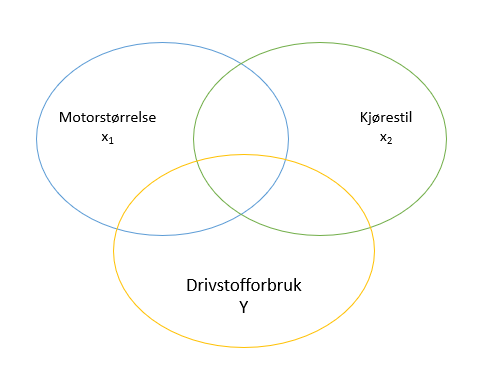
\includegraphics[width=0.5\textwidth,height=\textheight]{Venn1.png}

Den gule sirkelen illustrerer det forholdet vi er interessert i å ``finne ut noe om''. Den representerer det vi kaller den avhengige variabelen - fordi det vi ønsker å finne ut er avhengig av andre forhold (andre variabler). Vi kan si at den gule sirkelen viser variasjonen i drivstofforbruket til alle biler vi har med i undersøkelsen vår, og vi betegner denne variabelen \(Y\). Biler har ulikt drivstofforbruk, så vi har altså en variasjon i drivstofforbruket mellom bilene. Den blå sirkelen viser variasjonen i motorstørrelse (vi kaller denne variabelen for \(x_1\)). Ulike biler har ulik motorstørrelse, og vi tenker at større motor betyr mer drivstofforbruk enn mindre motor. Den grønne sirkelen representerer en variabel vi har kalt kjørestil (\(x_2\)).

Vi har en hypotese om at vi kan predikere (forutsi) drifstofforbruket til en gitt bil ut fra motorstørrelse og kjørestil. Så det vi ønsker å se på er hvor mye av korrelasjonen mellom drivstofforbruk og motorstørrelse skyldes faktisk motorstørrelse, og hvor mye skyldes kjørestil. Vi tenker også at kjørestil og drivstofforbruk er korrelert (det er naturlig å tenke seg at personer med en aggresiv kjørestil har biler med større motorer - det er altså en korrelasjon mellom kjørestil og motorstørrelse). Vi ser dette i figuren under. Korrelasjonen mellom drivstofforbruk og motorstørrelse er gitt i områdene merket 1 og 2. Korrelasjonen mellom drivstofforbruk og kjørestil er gitt i områdene 2 og 3. Korrelasjonen mellom kjørestil og motorstørrelse er gitt i 2 og 4.

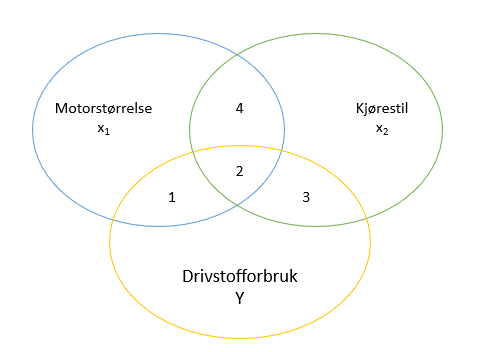
\includegraphics[width=0.5\textwidth,height=\textheight]{Venn2.png}

Området 2 viser den delte variasjonen mellom drivstofforbruk, motorstørrelse og kjørestil. Det vil innebære at vi kan bruke regresjonsanalsye til å isolere ut område 1 ved å se på motorstørrelsens totale korrelasjon med drivstofforbruk og trekke fra den delen av den totale korrelasjonen som deles med kjørestil (område 2). Da finner vi motorstørrelsens (\(x_1\)'s) unike bidrag.

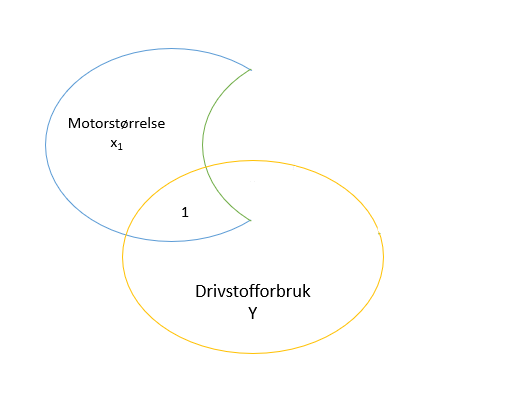
\includegraphics[width=0.5\textwidth,height=\textheight]{Venn3.png}

Det samme kan vi gjøre for kjørestil, der det unike bidraget utgjøres av område 3. Vi kan selvsagt ha flere prediktorer (uavhengige variabler) - noe vi veldig ofte vil ha. Det vi gjør er i prinsippet det samme: vi tar bort biter av korrelasjonen mellom motorstørrelse og drivstofforbruk som skyldes samvariasjon med andre variabler slik at vi får isolert den delen av korrelasjonen som utelukkende skyldes motorstørelse. Man kan tenke seg en ny variabel med rød sirkel. Igjen - regresjonsanalysen forsøker å isolere den unike delen for korrelasjonen mellom motorstørrelse og drivstofforbruk (og det samme for de andre variablene: den unike delen). Når vi klarer å isolere den unike korrelasjonen kan vi også si at vi har isolert den unike kausale effekten motorstørrelse har på drivstofforbruket (gitt at vi har inkludert alle relevant uavhengige variabler i modellen, noe vi i praksis sjelden vil klare).

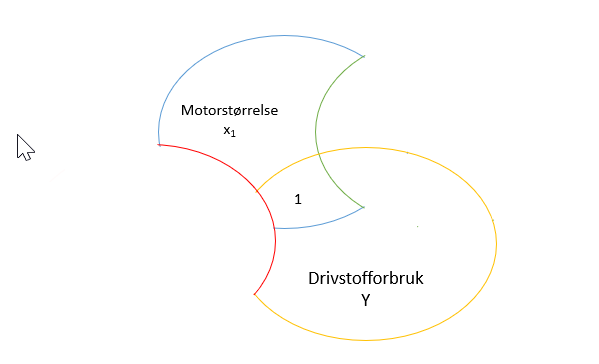
\includegraphics[width=0.5\textwidth,height=\textheight]{Venn5.png}

Den videre innledningen til regresjonsanalyse tar utgangspunkt i eksempelet i \citet{lovasStatistikkUniversiteterOg2013} (boka kom ut i 4. utgave i 2018). Illustrasjonene som er brukt er hentet fra bokas \href{www.nettressurser.no/statistikk}{nettressurser}. Løvås' bok «Statistikk for universiteter og høgskoler» kan anbefales som introduksjonsbok til statistikk på universitets- og høgskolenivået. En annen bok som fungerer fint til dette formålet er Jan Ubøes ``Statistikk for økonomifag'' (vi har brukt 4. utgave, 2014 - 5. utgave kom i 2015) \citep{uboeStatistikkOkonomifag2014}.

\hypertarget{teori}{%
\subsection{Teori}\label{teori}}

Eksempelet i \citet{lovasStatistikkUniversiteterOg2013} dreier seg om sammenhengen mellom motorstørrelse og drivstofforbruk. Vi kan måle motorstørrelse i hestekrefter (hk) og drivstofforbruk i liter/mil.

For å vise sammenhengen kan vi sette opp ligningen \(Y_i=\alpha\:+\beta x_i+e_i\) der

\(Y=drivstofforbruket\)

\(\alpha=konstantleddet\) (krysningspunktet på y-aksen, altså Y-verdien om x er 0)

\(\beta=linjens\:stigningstall\) (dersom x øker med 1, øker y med \(\beta\)

\(e=forstyrrelsen\) (vi antar at det er flere ting som forstyrrer forholdet mellom motorstørrelse og drivstofforbruk - drivstofforbruket er ikke bare avhengig av motorstørrelse). Vi skal snakke mye om residualer i regresjonsanalyse - residualer er dette restleddet/feilleddet/forstyrrelsen. En av forutsetningene i regresjonsanalyse er knyttet til fordelingen av disse residualene, men det kommer vi tilbake til.

Dersom vi ikke hadde hatt et feilledd kunne vi framstilt denne ligningen slik:

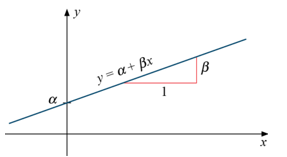
\includegraphics{Teori_fig1.png}

Når vi plotter inn et antall observasjoner av motorstørrelse og drivstofforbruk kan det se slik ut:

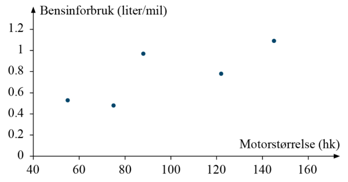
\includegraphics{Teori_fig2.png}

Det vi i en lineær regresjonsanalyse gjør er å finne den rette linja som best passer til disse observasjonene. Vi ønsker altså å finne en rett linje som best «beskriver» observasjonene. Tenk deg at vi trekker den rette linja som samlet sett ligger nærmest punktene og deretter tar bort punktene. Det vi sitter igjen med er regresjonslinja. Denne linja gir oss da ``tilgang til'' alle punkter som ligger på linja som en modell på sammenhengen mellom de to variablene. Selv om vi bare hadde noen observasjoner på gitte punkter på x-aksen har vi gjennom regresjonslinja fått tilgang til alle tenkelige punkter på x-linja og kan anta et drivstofforbruk ut fra det (ved å gå opp fra x-aksen, finne skjæringspunktet med regresjonslinja, og deretter gå inn på y-aksen og lese av drivstofforbruket). Den prediksjonen vi da gjør er vår beste gjetning på hvor stort drivstofforbruket vil være for en gitt motorstørrelse. Dette vil selvsagt være en kvalifisert gjetning - nettopp fordi det er en modell. Og alle modeller er feil, men noen modeller er nyttige likevel.

I eksempelet kan vi for eksempel tenke oss to mulige linjer:

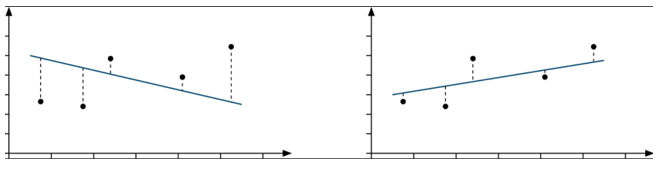
\includegraphics{Teori_fig3.png}

Begge linjene er forsøk på å lage en rett linje som har kortest mulig avvik. Vi kan deretter legge sammen de absolutte vertikale avstandene (de stiplede linjene) fra observasjonspunktene ned til den rette linja. I prinsippet er da den rette linja som medfører minst samlet avstand fra observasjonspunktene den rette linja som best representerer observasjonspunktene, og vi kan si vi har laget en modell for sammenhengen mellom motorstørrelse og drivstofforbruk. Siden vi har en sammenhengende rett linje har vi også mulighet til å mene noe om drivstofforbruk på motorstørrelser vi ikke har målt/har observasjoner på. Vi har med andre ord en modell for å predikere drivstofforbruk ut fra motorstørrelse. Uavhengige variabler i regresjonsanalyser kalles også ofte prediktorer, fordi vi bruker de til å predikere en verdi for den avhengige variabelen.

\hypertarget{minste-kvadratsum-ordinary-least-squares---ols}{%
\subsubsection{Minste kvadratsum (Ordinary Least Squares - OLS)}\label{minste-kvadratsum-ordinary-least-squares---ols}}

Imidlertid er absoluttverdier matematisk problematiske \citep{lovasStatistikkUniversiteterOg2013}. Pre-datamaskiner ble det derfor utviklet en alternativ måte som kalles «minste kvadraters metode» - derav begrepet OLS («Ordinary Least Squares»). Det finnes andre måter å tilnærme seg dette, men i dette kurset går vi kun inn på OLS-regresjon. Hvis vi fortsetter eksempelet over kan vi tenke oss en mengde forslag på ulike linjer som forsøker å beskrive sammenhengen mellom de to variablene:

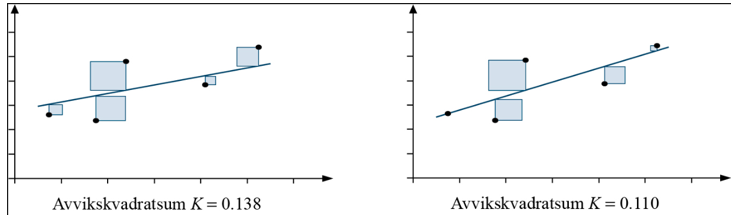
\includegraphics{Teori_fig4.png}

Man regner deretter ut kvadratene som dannes av hvert punkt og avstanden til den rette linja. Den linja som har den laveste kvadratsummen («least squares») er den linja som best representerer datapunktene og som derfor er den beste lineære modellen av forholdet mellom variablene. Regresjonslinja er således en modell. Som \citet{thraneAppliedRegressionAnalysis2019} beskriver: den diagonale linja oppsummerer den typiske trenden i det statistiske forholdet mellom de to variablene - en linje vi kjenner som regresjonslinja.
Hvis vi har et stort antall datapunkter er dette selvsagt en omfattende prosess å gjøre manuelt. Det statistikkprogrammer gjør for oss er å regne ut kvadratsummen for et stort antall mulige linjer og deretter fortelle oss hvilken som har lavest kvadratsum.

Hvis vi tenker tilbake til formelen for modellen vår: \(Y_i=\alpha\:+\beta x_i+e_i\) kan vi nå fylle ut med verdier fra eksempelet.

Det vi egentlig har gjort når vi finner den rette linja som gir minste kvadratsum er å identifisere \(\alpha\) (skjæringspunktet på y-aksen) og \(\beta\) (stigningstallet). Statistikkprogrammer vil gi oss verdiene på dette. Vi går ikke inn på en manuell utregning her, men bruker de to verdiene \citet{lovasStatistikkUniversiteterOg2013} viser (\(\alpha=0.211\) og \(\beta=0.00576\)). Vår modell ser da slik ut: \(Y_i=0,211\:+0,00576x_i\).

Som sagt har vi ønsket å lage en modell som predikerer drivstofforbruk ut fra motorstørrelse -- eller sagt på en annen måte: hvilket drivstofforbruk kan vi forvente med en motor på 100 hk? Vi får da: \[Y_i=0,211\:+0,00576x_i=0,211\:+\:0,00576\times100\:=\:0,787\]

Dette blir vårt ``best guess'', vår antakelse (vår prediksjon av verdien på y-aksen som er drivstofforbruket ut fra verdien på x-aksen som er motorstørrelse), om forventet drivstofforbruk for en motor med 100 hk basert på den modellen vi har laget om sammenhengen mellom motorstørrelse og drivstofforbruk (som er basert på de observasjonene vi har).

Vi kan naturligvis umiddelbart tenke at drivstofforbruket er avhengig av mange andre faktorer enn motorstørrelse, for eksempel bilens design (luftmotstand), vekt, rullemotstand, temperatur, type motor og så videre. Dette belyser for så vidt et sentralt problem når vi ønsker å lage modeller for prediksjon: Virkeligheten er utrolig sammensatt, mange relevante variabler er vanskelig å måle, og man ønsker en modell som er enkel nok til å kunne brukes og sammensatt nok til å gi relevante prediksjoner. Tenk for eksempel bare på «klimamodellene» som brukes for å analysere og predikere temperatur, issmelting, global oppvarming og liknende. Det er klart at i de fleste tilfeller trenger vi flere prediktorer enn en -- og i regresjonssammenheng snakker vi da om multippel regresjonsanalyse. Vi kan ha som en tommelfingerregel at vi skal ha med så mange variabler at modellen har praktisk verdi, men likevel så få som mulig.

\hypertarget{konfidensintervall}{%
\subsubsection{Konfidensintervall}\label{konfidensintervall}}

Avslutningsvis i denne introduksjonen til regresjonsanalyse kan vi se kort på begrepet konfidensintervall (se for eksempel \citet{lovasStatistikkUniversiteterOg2013} eller \citet{hinkleAppliedStatisticsBehavioral2003}). For de som ønsker å fordype seg i effektstørrelser og konfidensintervaller anbefales \citet{cummingIntroductionNewStatistics2017} ``Introduction to the new statistics: Estimation, open science, \& beyond''.

Man kan si at estimatet på stigningstallet \(\beta\) er det viktigste resultatet i en regresjonsanalyse fordi dette sier noe om hvor sterk sammenhengen mellom de to variablene er. \citet{lovasStatistikkUniversiteterOg2013} illustrerer dette slik:

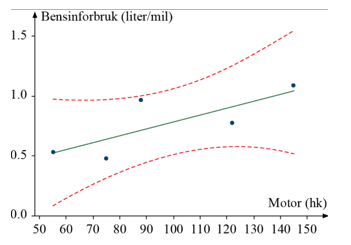
\includegraphics{Teori_fig5.png}

De røde stiplede linjene utgjør konfidensgrensene for 95 \% konfidensintervall. I grafen over har vi kun 5 observasjoner, noe som selvsagt er lite. Vi kan gå litt dypere inn i hvordan konfidensgrensene framkommer i en regresjonsanalyse.

La oss anta at vi har et datasett der vi har plottet korrelasjonen mellom en prediktor (den uavhengige variabelen) på x-aksen og en avhengig varaibel på y-aksen (se graf under). Den røde prikken markerer verdien x=8. Verdien på y-aksen (10,458) er vår prediksjon (vår buest guess) på hva verdien i den avhengige variabelen vil være ved den observerte verdien x=8.

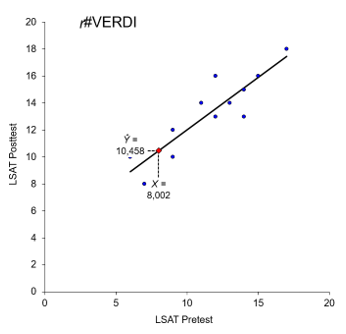
\includegraphics{Teori_fig6.png}

I punktet x=8 har vi en hel populasjon av mulige normalfordelte verdier. Vårt beste estimat av gjennomsnittsverdien for denne populasjonen er 10,458. Dette er et punktestimat. Det tilhørende intervallestimatet er vårt konfidensintervall. Vi må her tenke på konfidensintervallet som en vertikal linje. Så i stedet for å tenke punkt- og intervallestimat slik

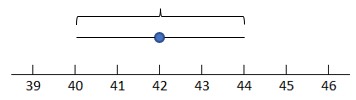
\includegraphics{Teori_fig7.png}

Kan vi tenke det slik:

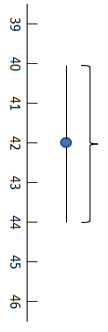
\includegraphics{Teori_fig8.png}

Overført til vårt eksempel får vi:

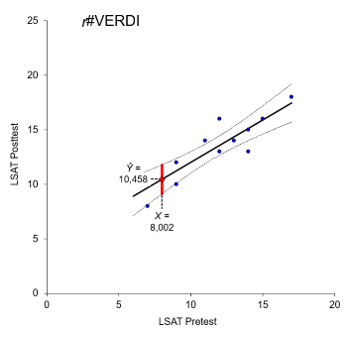
\includegraphics{Teori_fig9.png}

Den røde streken er vårt 95 \% konfidensintervall for punktestimatet. Hvis vi legger på 95 \% konfidensintervaller på alle punktestimatene (alle punktene som utgjør regresjonslinja) kan vi lage de to stiplede linjene som toucher endepunktene på alle konfidensintervallene. Disse to stiplede linjene utgjør da konfidensgrensene for regresjonslinja.

Vi ser at konfidensgrensene er lett buede mot hverandre med minst avstand mellom dem ``på midten''. Vi skal kort se på hvorfor det er slik. Vi har nå lagt på et nytt kryss i grafen under. Dette krysset markerer punktet der gjennomsnittene av X og Y krysser. Regresjonslinja må gå gjennom dette punktet, slik at alle alternative regresjonslinjer må pivotere rundt dette punktet. Dette medfører at det er litt større usikkerhet rundt punktestimatenes konfidensintervaller i endene i forhold til i midten. Konfidensintervallene for hvert enkelt punkt blir derfor litt lenger jo lenger ut fra krysningspunket vi går, og resultatet blir en form for buet linje.

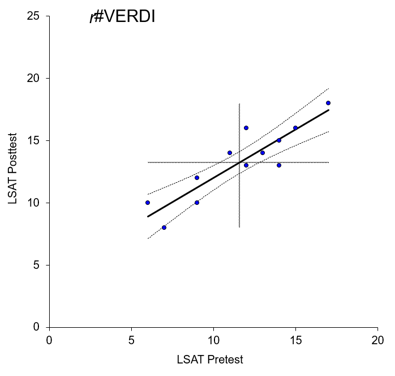
\includegraphics{Teori_fig10.png}

\hypertarget{steg-i-analyse}{%
\subsubsection{Steg i analyse}\label{steg-i-analyse}}

Vi anbefaler at en analyse går gjennom disse stegene:

\begin{enumerate}
\def\labelenumi{\arabic{enumi}.}
\item
  Analyse av dataene
\item
  Evtentuelt valg av prediktorer ut fra analyse av dataene
\item
  Lage modell (kjøre regresjonsanalysen)
\item
  Analyse av resultatene (diagnostikk)
\item
  Sjekk av forutsetningene
\item
  Eventuell revisjon av modellen
\item
  Eventuell analyse av revidert modell
\item
  Konklusjon / oppsummering / rapportering av resultater
\end{enumerate}

Vi skal i det følgende gå gjennom disse stegene i en regresjonsanalyse.

\hypertarget{enkel-lineuxe6r-regresjonsanalyse}{%
\subsection{Enkel, lineær regresjonsanalyse}\label{enkel-lineuxe6r-regresjonsanalyse}}

Dette eksempelet bygger på \citet{fieldDiscoveringStatisticsUsing2009}. Hvis vi ønsker å se på i hvilken grad vi kan predikere salgstall gjennom hvor mye vi bruker på reklame før lansering kan vi gjøre en lineær regresjonsanalyse med salg som avhengig variabel og reklame (adverts) som uavhengig variabel.

Du kan laste ned datasettet i ulike formater her:

Datasettet kan også finnes \href{https://edge.sagepub.com/field5e/student-resources/datasets}{her}

Vi skal nå gå gjennom våre anbefalte steg i analysen, og starter med en analyse av dataene.

\hypertarget{steg-1-analyse-av-dataene}{%
\subsubsection{Steg 1: Analyse av dataene}\label{steg-1-analyse-av-dataene}}

``As soon as you have collected your data, before you compute any statistics, look at your data. Data screening is not data snooping. It is not an opportunity to discard data or change values to favor your hypotheses. However, if you assess hypotheses without examining your data, you risk publishing nonsense'' \citep{wilkinsonStatisticalMethodsPsychology1999}.

Vi ser på datasettet og noen nøkkeltall for datasettet.

\begin{Shaded}
\begin{Highlighting}[]
\CommentTok{\# Bruker pakken: readxl}
\NormalTok{Field\_OLS\_data }\OtherTok{\textless{}{-}} \FunctionTok{read\_excel}\NormalTok{(}\StringTok{"Field\_datasett\_OLS.xlsx"}\NormalTok{)}
\CommentTok{\# Bruker pakken: summarytools}
\NormalTok{summarytools}\SpecialCharTok{::}\FunctionTok{descr}\NormalTok{(Field\_OLS\_data)}
\end{Highlighting}
\end{Shaded}

Descriptive Statistics\\
Field\_OLS\_data\\
N: 200

\begin{longtable}[]{@{}lrrrr@{}}
\toprule
& Adverts & Airplay & Image & Sales \\
\midrule
\endhead
Mean & 614.41 & 27.50 & 6.77 & 193.20 \\
Std.Dev & 485.66 & 12.27 & 1.40 & 80.70 \\
Min & 9.10 & 0.00 & 1.00 & 10.00 \\
Q1 & 215.84 & 19.50 & 6.00 & 135.00 \\
Median & 531.92 & 28.00 & 7.00 & 200.00 \\
Q3 & 911.60 & 36.00 & 8.00 & 250.00 \\
Max & 2271.86 & 63.00 & 10.00 & 360.00 \\
MAD & 489.09 & 11.86 & 1.48 & 88.96 \\
IQR & 695.31 & 16.25 & 2.00 & 112.50 \\
CV & 0.79 & 0.45 & 0.21 & 0.42 \\
Skewness & 0.84 & 0.06 & -1.27 & 0.04 \\
SE.Skewness & 0.17 & 0.17 & 0.17 & 0.17 \\
Kurtosis & 0.17 & -0.09 & 3.56 & -0.72 \\
N.Valid & 200.00 & 200.00 & 200.00 & 200.00 \\
Pct.Valid & 100.00 & 100.00 & 100.00 & 100.00 \\
\bottomrule
\end{longtable}

Vi kan se at datasettet består av 200 obervasjoner av 4 variabler. Hver av observasjonene er en CD:

\begin{itemize}
\tightlist
\item
  Adverts: Dette er summen brukt på reklame før lanseringsdato
\item
  Sales: Dette er salgtall per uke
\item
  Airplay: Antall ganger et spor fra CDen ble spilt på radio i uka før lanseringsdato
\item
  Image: En rating på hvor attraktiv gruppen/artisten (positivt image)
\end{itemize}

Ofte er det imidlertid mer hensiktsmessig å se på dataene grafisk i en utforskende hensikt \citep{tukeyExploratoryDataAnalysis1977}.

\hypertarget{histogram}{%
\paragraph{Histogram}\label{histogram}}

\begin{Shaded}
\begin{Highlighting}[]
\CommentTok{\# Bruker pakkene: ggplot2 og gridExtra}

\NormalTok{annotations }\OtherTok{\textless{}{-}} \FunctionTok{data.frame}\NormalTok{(}
  \AttributeTok{x =} \FunctionTok{c}\NormalTok{(}\FunctionTok{round}\NormalTok{(}\FunctionTok{min}\NormalTok{(Field\_OLS\_data}\SpecialCharTok{$}\NormalTok{Adverts), }\DecValTok{2}\NormalTok{), }\FunctionTok{round}\NormalTok{(}\FunctionTok{mean}\NormalTok{(Field\_OLS\_data}\SpecialCharTok{$}\NormalTok{Adverts), }\DecValTok{2}\NormalTok{), }\FunctionTok{round}\NormalTok{(}\FunctionTok{max}\NormalTok{(Field\_OLS\_data}\SpecialCharTok{$}\NormalTok{Adverts), }\DecValTok{2}\NormalTok{)),}
  \AttributeTok{y =} \FunctionTok{c}\NormalTok{(}\DecValTok{4}\NormalTok{, }\DecValTok{52}\NormalTok{, }\DecValTok{5}\NormalTok{),}
  \AttributeTok{label =} \FunctionTok{c}\NormalTok{(}\StringTok{"Min:"}\NormalTok{, }\StringTok{"Gjennomsnitt:"}\NormalTok{, }\StringTok{"Maks:"}\NormalTok{))}
  
\NormalTok{plott1 }\OtherTok{\textless{}{-}} \FunctionTok{ggplot}\NormalTok{(Field\_OLS\_data, }\FunctionTok{aes}\NormalTok{(Adverts)) }\SpecialCharTok{+} 
  \FunctionTok{geom\_histogram}\NormalTok{(}\AttributeTok{bins =} \DecValTok{10}\NormalTok{, }\AttributeTok{color =} \StringTok{"\#000000"}\NormalTok{, }\AttributeTok{fill =} \StringTok{"\#0099F8"}\NormalTok{) }\SpecialCharTok{+} 
    \FunctionTok{geom\_vline}\NormalTok{(}\FunctionTok{aes}\NormalTok{(}\AttributeTok{xintercept =} \FunctionTok{mean}\NormalTok{(Adverts)), }\AttributeTok{color =} \StringTok{"\#000000"}\NormalTok{, }\AttributeTok{size =} \FloatTok{0.5}\NormalTok{, }\AttributeTok{linetype =} \StringTok{"dashed"}\NormalTok{) }\SpecialCharTok{+} 
 \FunctionTok{geom\_text}\NormalTok{(}\AttributeTok{data =}\NormalTok{ annotations, }\FunctionTok{aes}\NormalTok{(}\AttributeTok{x =}\NormalTok{ x, }\AttributeTok{y =}\NormalTok{ y, }\AttributeTok{label =} \FunctionTok{paste}\NormalTok{(label, x)), }\AttributeTok{size =} \DecValTok{2}\NormalTok{, }\AttributeTok{fontface =} \StringTok{"bold"}\NormalTok{) }\SpecialCharTok{+}
      \FunctionTok{theme\_classic}\NormalTok{()}

\NormalTok{annotations2 }\OtherTok{\textless{}{-}} \FunctionTok{data.frame}\NormalTok{(}
  \AttributeTok{x =} \FunctionTok{c}\NormalTok{(}\FunctionTok{round}\NormalTok{(}\FunctionTok{min}\NormalTok{(Field\_OLS\_data}\SpecialCharTok{$}\NormalTok{Sales), }\DecValTok{2}\NormalTok{), }\FunctionTok{round}\NormalTok{(}\FunctionTok{mean}\NormalTok{(Field\_OLS\_data}\SpecialCharTok{$}\NormalTok{Sales), }\DecValTok{2}\NormalTok{), }\FunctionTok{round}\NormalTok{(}\FunctionTok{max}\NormalTok{(Field\_OLS\_data}\SpecialCharTok{$}\NormalTok{Sales), }\DecValTok{2}\NormalTok{)),}
  \AttributeTok{y =} \FunctionTok{c}\NormalTok{(}\DecValTok{4}\NormalTok{, }\DecValTok{52}\NormalTok{, }\DecValTok{5}\NormalTok{),}
  \AttributeTok{label =} \FunctionTok{c}\NormalTok{(}\StringTok{"Min:"}\NormalTok{, }\StringTok{"Gjennomsnitt:"}\NormalTok{, }\StringTok{"Maks:"}\NormalTok{))}

\NormalTok{plott2 }\OtherTok{\textless{}{-}} \FunctionTok{ggplot}\NormalTok{(Field\_OLS\_data, }\FunctionTok{aes}\NormalTok{(Sales)) }\SpecialCharTok{+} 
  \FunctionTok{geom\_histogram}\NormalTok{(}\AttributeTok{bins =} \DecValTok{10}\NormalTok{, }\AttributeTok{color =} \StringTok{"\#000000"}\NormalTok{, }\AttributeTok{fill =} \StringTok{"\#0099F8"}\NormalTok{) }\SpecialCharTok{+} 
    \FunctionTok{geom\_vline}\NormalTok{(}\FunctionTok{aes}\NormalTok{(}\AttributeTok{xintercept =} \FunctionTok{mean}\NormalTok{(Sales)), }\AttributeTok{color =} \StringTok{"\#000000"}\NormalTok{, }\AttributeTok{size =} \FloatTok{0.5}\NormalTok{, }\AttributeTok{linetype =} \StringTok{"dashed"}\NormalTok{) }\SpecialCharTok{+} 
 \FunctionTok{geom\_text}\NormalTok{(}\AttributeTok{data =}\NormalTok{ annotations2, }\FunctionTok{aes}\NormalTok{(}\AttributeTok{x =}\NormalTok{ x, }\AttributeTok{y =}\NormalTok{ y, }\AttributeTok{label =} \FunctionTok{paste}\NormalTok{(label, x)), }\AttributeTok{size =} \DecValTok{2}\NormalTok{, }\AttributeTok{fontface =} \StringTok{"bold"}\NormalTok{) }\SpecialCharTok{+}
      \FunctionTok{theme\_classic}\NormalTok{()}
\FunctionTok{grid.arrange}\NormalTok{(plott1, plott2, }\AttributeTok{ncol=}\DecValTok{2}\NormalTok{)}
\end{Highlighting}
\end{Shaded}

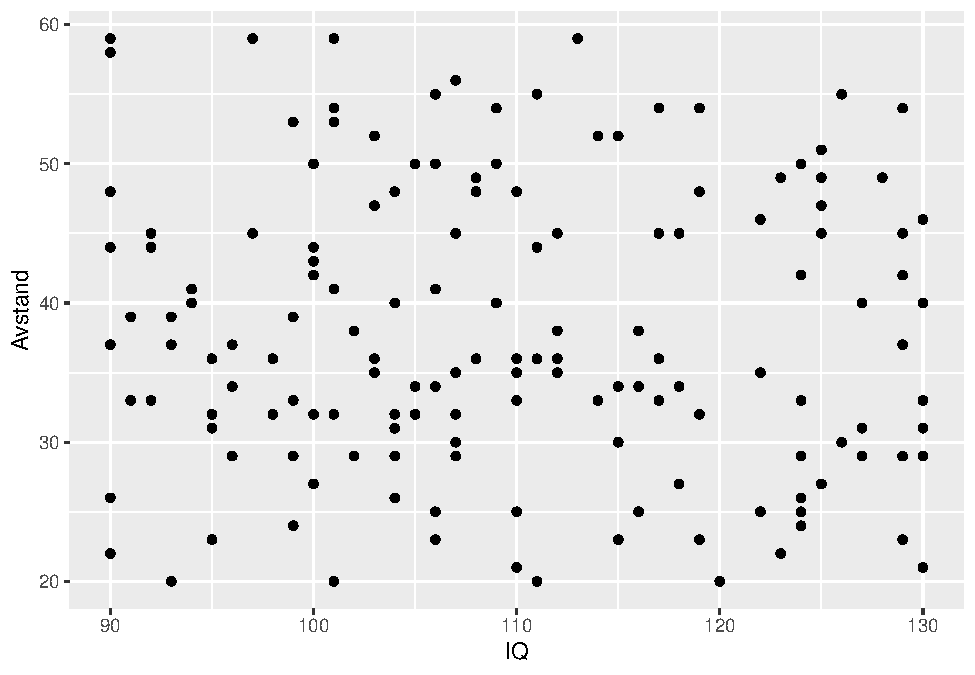
\includegraphics{02_Kap_2_files/figure-latex/unnamed-chunk-6-1.pdf}

Det kan se ut som at salgstallene er rimelig normalfordelte, mens reklamevariabelen er klart skjev.

\hypertarget{quantile-quantile-plott-qq}{%
\paragraph{Quantile-Quantile plott (qq)}\label{quantile-quantile-plott-qq}}

Q-Q plottet (``quantile-quantile plot'') kan tolkes ved å se om dataverdiene ligger langs en rett linje med ca 45 graders vinkel. Q-Q plottet innebærer å se to distribusjoner mot hverandre -- empirisk fordeling (dataene) og teoretisk forventning ut fra en fordelingsmodell (som normalfordeling om vi snakker om ``normal Q-Q plott'' - dvs vi ser om vår empiriske datafordeling og normalfordelingen er lik). Om de samsvarer perfekt ligger de på en helt rett linje (x = y). I eksempelet under vil da alle punktene ligge perfekt oppå den rette linjen. Siden vi vet den teoretiske distribusjonen til normalfordelingen, kan vi bruke denne teoretiske fordelingen til å plotte den mot datasettet vi sitter med.

\begin{Shaded}
\begin{Highlighting}[]
\CommentTok{\# Bruker pakken: car}
\FunctionTok{par}\NormalTok{(}\AttributeTok{mfrow=}\NormalTok{(}\FunctionTok{c}\NormalTok{(}\DecValTok{1}\NormalTok{,}\DecValTok{2}\NormalTok{)))}
\NormalTok{qqSales2 }\OtherTok{\textless{}{-}}\NormalTok{ car}\SpecialCharTok{::}\FunctionTok{qqPlot}\NormalTok{(Field\_OLS\_data}\SpecialCharTok{$}\NormalTok{Adverts)}
\NormalTok{qqAdverts2 }\OtherTok{\textless{}{-}}\NormalTok{ car}\SpecialCharTok{::}\FunctionTok{qqPlot}\NormalTok{(Field\_OLS\_data}\SpecialCharTok{$}\NormalTok{Sales)}
\end{Highlighting}
\end{Shaded}

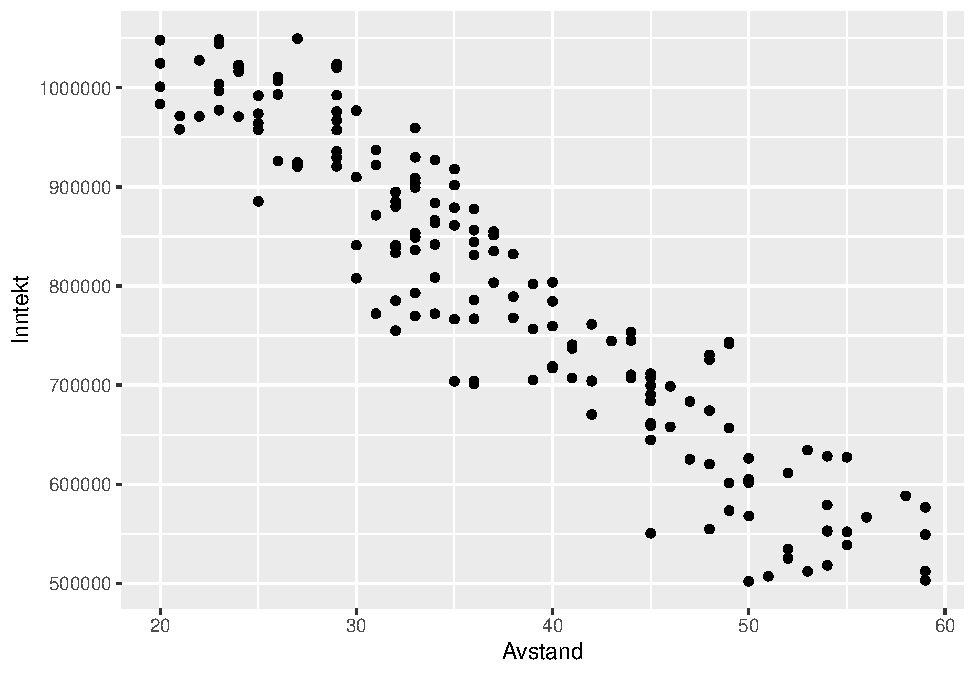
\includegraphics{02_Kap_2_files/figure-latex/unnamed-chunk-7-1.pdf}

Som vi fikk indikert gjennom historgrammene er salgsvariabelen rimelig normalfordelt, mens reklamevariabelen viser avvik fra normalfordelingen - i dette tilfellet (ut fra histogram og qq-plott vil vi si den er høyreskjev).

Under viser vi typiske mønstre for histogram og ``tilhørende'' qq-plott som kan være til hjelp i tolkning av dataene dine. Dette er genererte tall og ikke tallene fra eksempelet over:

\hypertarget{normalfordelt}{%
\subparagraph{Normalfordelt}\label{normalfordelt}}

\begin{Shaded}
\begin{Highlighting}[]
\FunctionTok{set.seed}\NormalTok{(}\DecValTok{89}\NormalTok{)}
\CommentTok{\# base R}
\CommentTok{\# Bruker pakken: tibble (Tidyverse)}
\NormalTok{qqnorm }\OtherTok{\textless{}{-}} \FunctionTok{as\_tibble}\NormalTok{(}\FunctionTok{rnorm}\NormalTok{(}\DecValTok{10000}\NormalTok{, }\AttributeTok{mean=}\DecValTok{90}\NormalTok{, }\AttributeTok{sd=}\DecValTok{5}\NormalTok{))}
\CommentTok{\# Bruker pakken: writexl}
\FunctionTok{write\_xlsx}\NormalTok{(qqnorm,}\StringTok{"QQ\_norm.xlsx"}\NormalTok{)}
\end{Highlighting}
\end{Shaded}

\begin{Shaded}
\begin{Highlighting}[]
\CommentTok{\# Bruker pakken: ggpubr}
\FunctionTok{ggqqplot}\NormalTok{(qqnorm}\SpecialCharTok{$}\NormalTok{value) }\SpecialCharTok{+} \FunctionTok{ggtitle}\NormalTok{(}\StringTok{"Normal Q{-}Q plott"}\NormalTok{) }\SpecialCharTok{+} \FunctionTok{labs}\NormalTok{(}\AttributeTok{x =} \StringTok{"Teoretisk forventning"}\NormalTok{, }\AttributeTok{y =} \StringTok{"Data"}\NormalTok{)}
\end{Highlighting}
\end{Shaded}

\begin{figure}
\centering
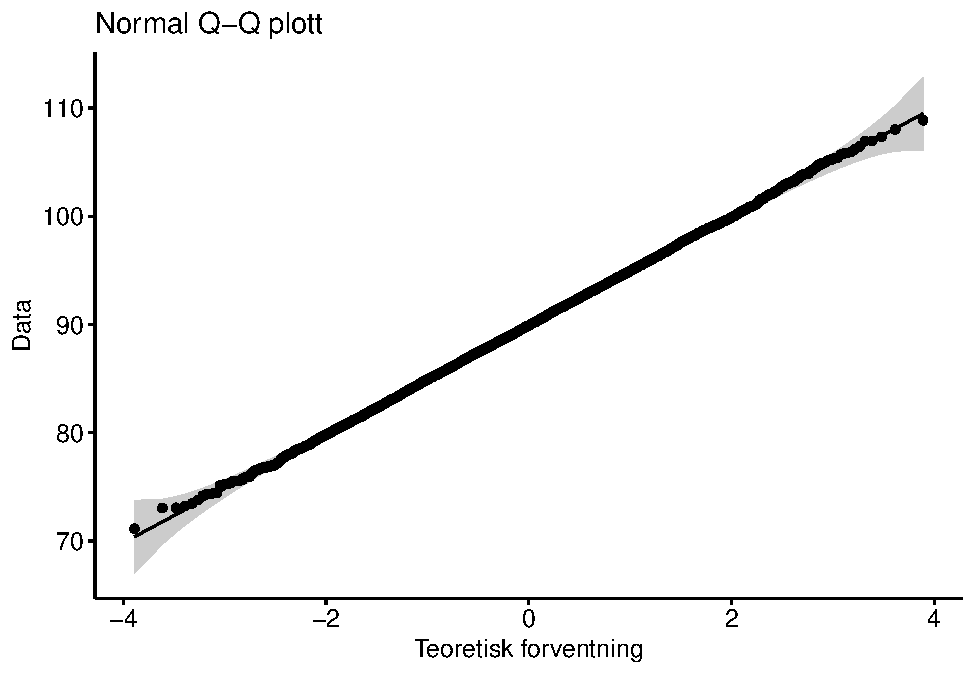
\includegraphics{02_Kap_2_files/figure-latex/unnamed-chunk-10-1.pdf}
\caption{\label{fig:unnamed-chunk-10}Q-Q plott normalfordeling}
\end{figure}

Vi ser at dette Q-Q plottet viser oss at vi kan være ganske sikre på at dette datasettet er normalfordelt (noe som gir meninig siden vi har brukt R til å lage et normalfordelt datasett).

\hypertarget{skjevhet-huxf8yre}{%
\subparagraph{Skjevhet høyre}\label{skjevhet-huxf8yre}}

\begin{Shaded}
\begin{Highlighting}[]
\CommentTok{\# Lage datasett med right skew}
\CommentTok{\# base R}
\CommentTok{\# Bruker pakken: tibble}
\FunctionTok{set.seed}\NormalTok{(}\DecValTok{90}\NormalTok{)}
\NormalTok{N }\OtherTok{\textless{}{-}} \DecValTok{5000}
\NormalTok{qqrightskew }\OtherTok{\textless{}{-}} \FunctionTok{as\_tibble}\NormalTok{(}\FunctionTok{rnbinom}\NormalTok{(N, }\DecValTok{10}\NormalTok{, .}\DecValTok{1}\NormalTok{))}
\CommentTok{\# Eksportere datasettet}
\CommentTok{\# Bruker pakken: writexl}
\FunctionTok{write\_xlsx}\NormalTok{(qqrightskew,}\StringTok{"QQ\_norm\_rs.xlsx"}\NormalTok{)}
\end{Highlighting}
\end{Shaded}

\begin{Shaded}
\begin{Highlighting}[]
\CommentTok{\# Plotte histogram og Q{-}Q plott"}
\CommentTok{\# Bruker pakken: ggplot2}
\NormalTok{qqrighthist }\OtherTok{\textless{}{-}} \FunctionTok{ggplot}\NormalTok{(qqrightskew, }\FunctionTok{aes}\NormalTok{(}\AttributeTok{x=}\NormalTok{value)) }\SpecialCharTok{+} \FunctionTok{geom\_histogram}\NormalTok{(}\AttributeTok{color=}\StringTok{"black"}\NormalTok{, }\AttributeTok{fill=}\StringTok{"lightblue"}\NormalTok{)}
\CommentTok{\# Bruker pakken: ggpubr}
\NormalTok{qqrightskew\_plott }\OtherTok{\textless{}{-}} \FunctionTok{ggqqplot}\NormalTok{(qqrightskew}\SpecialCharTok{$}\NormalTok{value) }\SpecialCharTok{+} \FunctionTok{ggtitle}\NormalTok{(}\StringTok{"Normal Q{-}Q plott {-} skjevhet høyre"}\NormalTok{) }\SpecialCharTok{+} \FunctionTok{labs}\NormalTok{(}\AttributeTok{x =} \StringTok{"Teoretisk forventning"}\NormalTok{, }\AttributeTok{y =} \StringTok{"Data"}\NormalTok{)}
\CommentTok{\# Bruker pakken: gridExtra}
\FunctionTok{grid.arrange}\NormalTok{(qqrighthist, qqrightskew\_plott, }\AttributeTok{ncol=}\DecValTok{2}\NormalTok{)}
\end{Highlighting}
\end{Shaded}

\begin{figure}
\centering
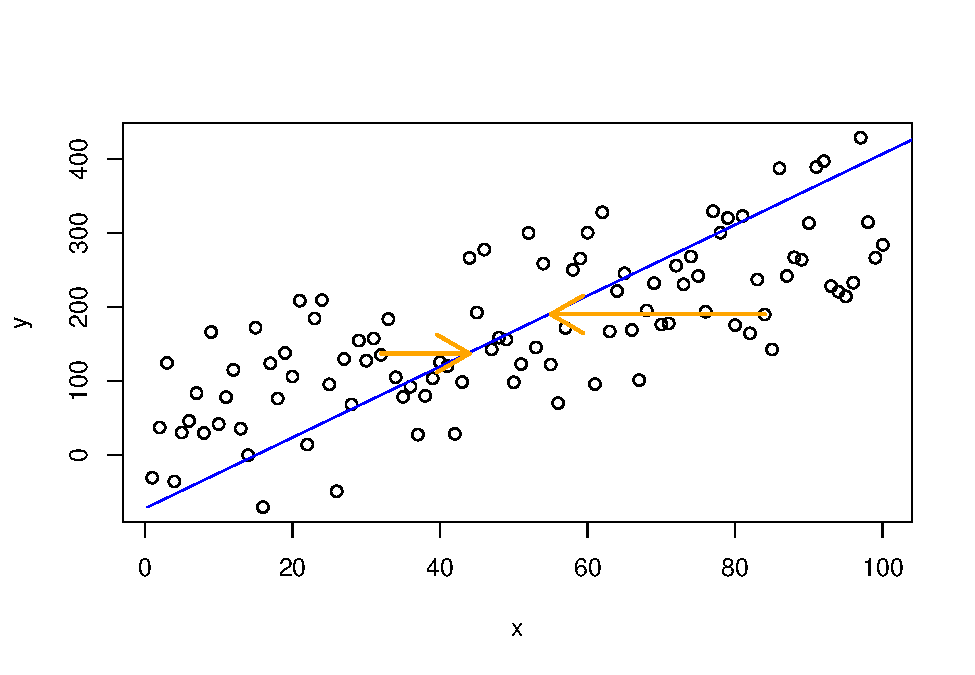
\includegraphics{02_Kap_2_files/figure-latex/unnamed-chunk-13-1.pdf}
\caption{\label{fig:unnamed-chunk-13}Q-Q plott - fordeling skjevhet høyre}
\end{figure}

I et datasett med høyreskjevhet vil ofte Q-Q plottet vise en bananform med bunnen/midten av bananen ned mot høyre hjørne og endene pekende oppover/utover fra den rette linjen.

\hypertarget{skjevhet-venstre}{%
\subparagraph{Skjevhet venstre}\label{skjevhet-venstre}}

\begin{Shaded}
\begin{Highlighting}[]
\CommentTok{\# Lage datasett med left skew}
\CommentTok{\# base R}
\CommentTok{\# Bruker pakken: tibble}
\FunctionTok{set.seed}\NormalTok{(}\DecValTok{91}\NormalTok{)}
\NormalTok{N}\OtherTok{=}\DecValTok{5000}
\NormalTok{qqleftskew }\OtherTok{\textless{}{-}} \FunctionTok{as\_tibble}\NormalTok{(}\FunctionTok{rbeta}\NormalTok{(N,}\DecValTok{5}\NormalTok{,}\DecValTok{1}\NormalTok{,}\AttributeTok{ncp=}\DecValTok{0}\NormalTok{))}
\CommentTok{\# Eksportere datasettet}
\CommentTok{\# Bruker pakken: writexl}
\FunctionTok{write\_xlsx}\NormalTok{(qqleftskew,}\StringTok{"QQ\_norm\_ls.xlsx"}\NormalTok{)}
\end{Highlighting}
\end{Shaded}

\begin{Shaded}
\begin{Highlighting}[]
\CommentTok{\# Plotte histogram og Q{-}Q plott}
\CommentTok{\# Bruker pakken: ggplot2}
\NormalTok{qqlefthist }\OtherTok{\textless{}{-}} \FunctionTok{ggplot}\NormalTok{(qqleftskew, }\FunctionTok{aes}\NormalTok{(}\AttributeTok{x=}\NormalTok{value)) }\SpecialCharTok{+} \FunctionTok{geom\_histogram}\NormalTok{(}\AttributeTok{color=}\StringTok{"black"}\NormalTok{, }\AttributeTok{fill=}\StringTok{"lightblue"}\NormalTok{)}
\CommentTok{\# Bruker pakken: ggpubr}
\NormalTok{qqleftskew\_plott }\OtherTok{\textless{}{-}} \FunctionTok{ggqqplot}\NormalTok{(qqleftskew}\SpecialCharTok{$}\NormalTok{value) }\SpecialCharTok{+} \FunctionTok{ggtitle}\NormalTok{(}\StringTok{"Normal Q{-}Q plott {-} skjevhet venstre"}\NormalTok{) }\SpecialCharTok{+} \FunctionTok{labs}\NormalTok{(}\AttributeTok{x =} \StringTok{"Teoretisk forventning"}\NormalTok{, }\AttributeTok{y =} \StringTok{"Data"}\NormalTok{)}
\CommentTok{\# Bruker pakken: gridExtra}
\FunctionTok{grid.arrange}\NormalTok{(qqlefthist, qqleftskew\_plott, }\AttributeTok{ncol=}\DecValTok{2}\NormalTok{)}
\end{Highlighting}
\end{Shaded}

\begin{figure}
\centering
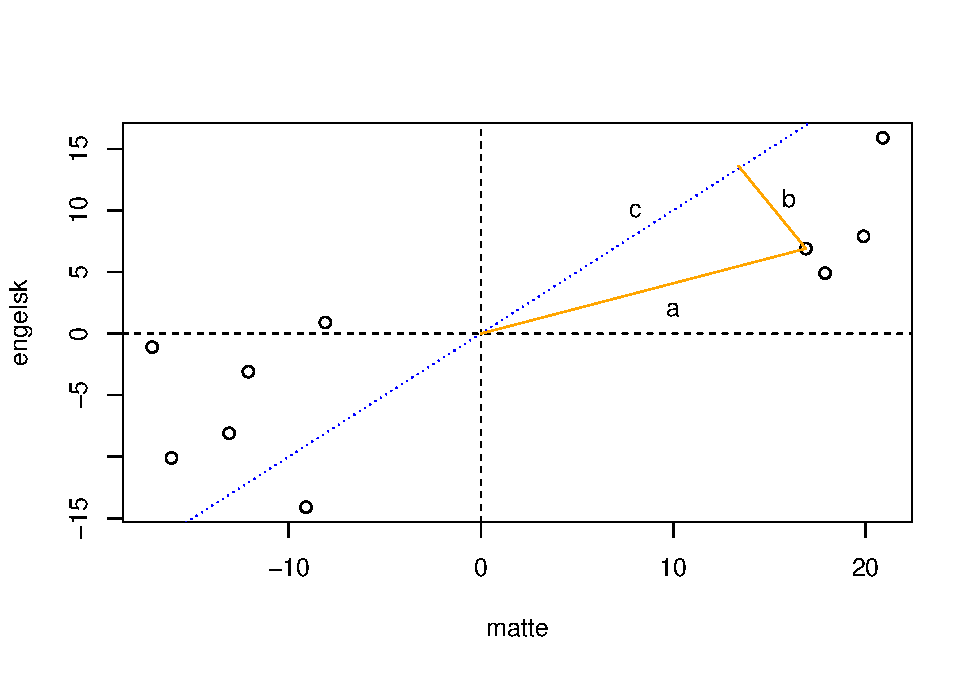
\includegraphics{02_Kap_2_files/figure-latex/unnamed-chunk-16-1.pdf}
\caption{\label{fig:unnamed-chunk-16}Q-Q plott - fordeling skjevhet venstre}
\end{figure}

I dette datasettet har vi generert en kraftig skjevhet til venstre. Q-Q plottet får da en omvendt bananform i forhold til høyre skjevhet, altså en topp på midten og to ender som svinger nedover ift den rette linja.

\hypertarget{tunge-haler}{%
\subparagraph{Tunge haler}\label{tunge-haler}}

\begin{Shaded}
\begin{Highlighting}[]
\FunctionTok{set.seed}\NormalTok{(}\DecValTok{14}\NormalTok{)}
\NormalTok{N}\OtherTok{=}\DecValTok{100}
\CommentTok{\# Bruker pakken: tibble}
\CommentTok{\# Base R}
\NormalTok{qqcauchy }\OtherTok{\textless{}{-}} \FunctionTok{as\_tibble}\NormalTok{(}\FunctionTok{rcauchy}\NormalTok{(N, }\AttributeTok{scale =} \DecValTok{5}\NormalTok{)) }
\CommentTok{\# Eksportere datasettet}
\CommentTok{\# Bruker pakken: writexl}
\FunctionTok{write\_xlsx}\NormalTok{(qqcauchy,}\StringTok{"QQ\_ht.xlsx"}\NormalTok{)}
\end{Highlighting}
\end{Shaded}

\begin{Shaded}
\begin{Highlighting}[]
\CommentTok{\# Bruker pakken: ggplot2}
\NormalTok{qqcauchyhist }\OtherTok{\textless{}{-}} \FunctionTok{ggplot}\NormalTok{(qqcauchy, }\FunctionTok{aes}\NormalTok{(}\AttributeTok{x=}\NormalTok{value)) }\SpecialCharTok{+} \FunctionTok{geom\_histogram}\NormalTok{(}\AttributeTok{color=}\StringTok{"black"}\NormalTok{, }\AttributeTok{fill=}\StringTok{"lightblue"}\NormalTok{)}
\CommentTok{\# Bruker pakken: ggpubr}
\NormalTok{qqcauchy\_plott }\OtherTok{\textless{}{-}} \FunctionTok{ggqqplot}\NormalTok{(qqcauchy}\SpecialCharTok{$}\NormalTok{value) }\SpecialCharTok{+} \FunctionTok{ggtitle}\NormalTok{(}\StringTok{"Normal Q{-}Q plott {-} tung hale"}\NormalTok{) }\SpecialCharTok{+} \FunctionTok{labs}\NormalTok{(}\AttributeTok{x =} \StringTok{"Teoretisk forventning"}\NormalTok{, }\AttributeTok{y =} \StringTok{"Data"}\NormalTok{)}
\CommentTok{\# Bruker pakken: gridExtra}
\FunctionTok{grid.arrange}\NormalTok{(qqcauchyhist, qqcauchy\_plott, }\AttributeTok{ncol=}\DecValTok{2}\NormalTok{)}
\end{Highlighting}
\end{Shaded}

\begin{figure}
\centering
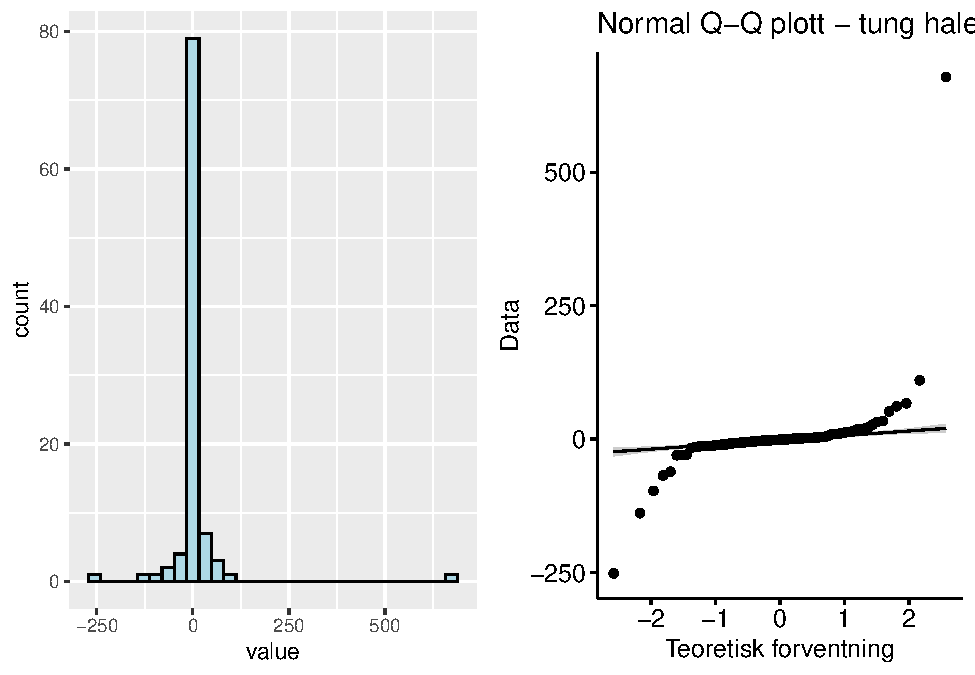
\includegraphics{02_Kap_2_files/figure-latex/unnamed-chunk-19-1.pdf}
\caption{\label{fig:unnamed-chunk-19}Q-Q plott - `heavy-tail'}
\end{figure}

``Heavy-tailed'' (fete/tunge haler) har større sannsynlighet for at ekstreme verdier vil forekomme). Fordelinger med tunge haler vil ofte følge en slags S-form, men den er ofte mer ``liggende'' enn S-formen til fordeling med lette haler. Den starter med å vokse raskere enn normalfordelingen og ender med å vokse saktere.

\hypertarget{lette-haler}{%
\subparagraph{Lette haler}\label{lette-haler}}

\begin{Shaded}
\begin{Highlighting}[]
\FunctionTok{set.seed}\NormalTok{(}\DecValTok{81}\NormalTok{)}
\CommentTok{\# Base R}
\CommentTok{\# Bruker pakken: tibble}
\NormalTok{qqlt }\OtherTok{\textless{}{-}} \FunctionTok{as\_tibble}\NormalTok{(}\FunctionTok{runif}\NormalTok{(}\AttributeTok{n =} \DecValTok{1000}\NormalTok{, }\AttributeTok{min =} \SpecialCharTok{{-}}\DecValTok{1}\NormalTok{, }\AttributeTok{max =} \DecValTok{1}\NormalTok{))}
\CommentTok{\# Eksportere datasettet}
\CommentTok{\# Bruker pakken: writexl}
\FunctionTok{write\_xlsx}\NormalTok{(qqlt,}\StringTok{"QQ\_lt.xlsx"}\NormalTok{)}
\end{Highlighting}
\end{Shaded}

\begin{Shaded}
\begin{Highlighting}[]
\CommentTok{\# Bruker pakken: ggplot2}
\NormalTok{qqlthist }\OtherTok{\textless{}{-}} \FunctionTok{ggplot}\NormalTok{(qqlt, }\FunctionTok{aes}\NormalTok{(}\AttributeTok{x=}\NormalTok{value)) }\SpecialCharTok{+} \FunctionTok{geom\_histogram}\NormalTok{(}\AttributeTok{color=}\StringTok{"black"}\NormalTok{, }\AttributeTok{fill=}\StringTok{"lightblue"}\NormalTok{)}
\CommentTok{\# Bruker pakken ggpubr}
\NormalTok{qqlt\_plott }\OtherTok{\textless{}{-}} \FunctionTok{ggqqplot}\NormalTok{(qqlt}\SpecialCharTok{$}\NormalTok{value) }\SpecialCharTok{+} \FunctionTok{ggtitle}\NormalTok{(}\StringTok{"Normal Q{-}Q plott {-} lett hale"}\NormalTok{) }\SpecialCharTok{+} \FunctionTok{labs}\NormalTok{(}\AttributeTok{x =} \StringTok{"Teoretisk forventning"}\NormalTok{, }\AttributeTok{y =} \StringTok{"Data"}\NormalTok{)}
\CommentTok{\# Bruker pakken: gridExtra}
\FunctionTok{grid.arrange}\NormalTok{(qqlthist, qqlt\_plott, }\AttributeTok{ncol=}\DecValTok{2}\NormalTok{)}
\end{Highlighting}
\end{Shaded}

\begin{figure}
\centering
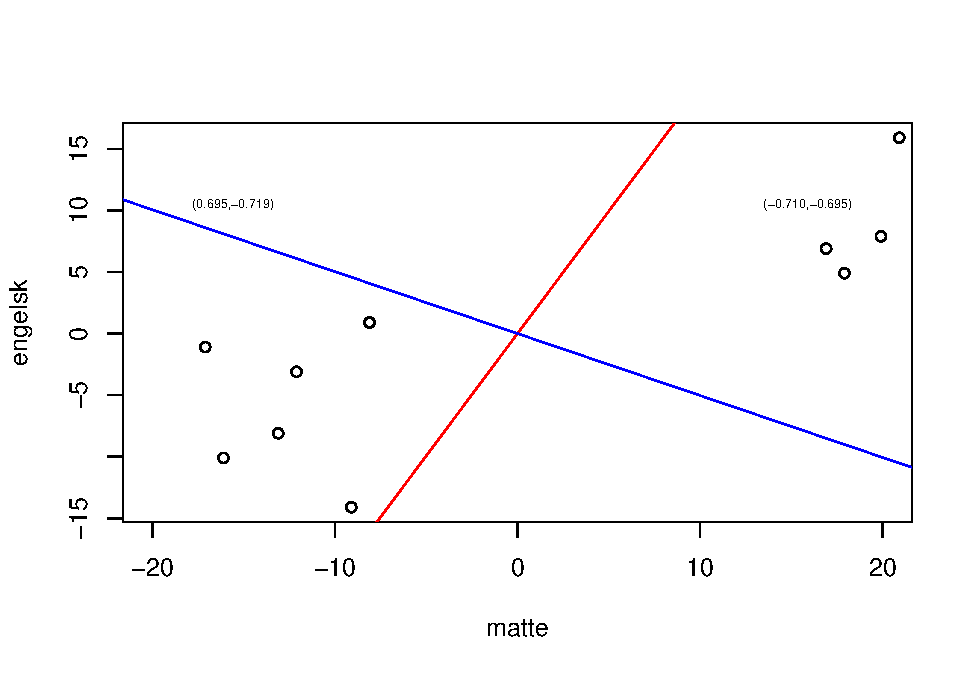
\includegraphics{02_Kap_2_files/figure-latex/unnamed-chunk-22-1.pdf}
\caption{\label{fig:unnamed-chunk-22}Q-Q plott - `light-tail'}
\end{figure}

``Light-tailed'' (lette haler) har liten sannsynlighet for ekstreme verdier og utvalg tenderer til å ikke fravike gjennomsnittet med mye. Q-Q plottet for en fordeling med lette haler har ofte en S-form. Dataene vokser saktere enn normalfordelingen i starten før den følger vekstraten til normalfordelingen. Mot slutten vokser den raskere enn normalfordelingen. Derfor bøyer den av fra normalfordelingen.

\hypertarget{bimodalitet}{%
\subparagraph{Bimodalitet}\label{bimodalitet}}

\begin{Shaded}
\begin{Highlighting}[]
\FunctionTok{set.seed}\NormalTok{(}\DecValTok{10}\NormalTok{) }
\CommentTok{\# Base R}
\CommentTok{\# Bruker pakken: ggplot2}
\CommentTok{\# Bruker pakken: tibble}
\NormalTok{mode1 }\OtherTok{\textless{}{-}} \FunctionTok{rnorm}\NormalTok{(}\DecValTok{50}\NormalTok{,}\DecValTok{2}\NormalTok{,}\DecValTok{1}\NormalTok{)}
\NormalTok{mode1 }\OtherTok{\textless{}{-}}\NormalTok{ mode1[mode1 }\SpecialCharTok{\textgreater{}} \DecValTok{0}\NormalTok{] }
\NormalTok{mode2 }\OtherTok{\textless{}{-}} \FunctionTok{rnorm}\NormalTok{(}\DecValTok{50}\NormalTok{,}\DecValTok{6}\NormalTok{,}\DecValTok{1}\NormalTok{)}
\NormalTok{mode2 }\OtherTok{\textless{}{-}}\NormalTok{ mode2[mode2 }\SpecialCharTok{\textgreater{}} \DecValTok{0}\NormalTok{] }
\NormalTok{qqbimod }\OtherTok{\textless{}{-}} \FunctionTok{as\_tibble}\NormalTok{(}\FunctionTok{sort}\NormalTok{(}\FunctionTok{c}\NormalTok{(mode1,mode2)))}
\CommentTok{\# Eksportere datasettet}
\CommentTok{\# Bruker pakken: writexl}
\FunctionTok{write\_xlsx}\NormalTok{(qqbimod,}\StringTok{"QQ\_bimod.xlsx"}\NormalTok{)}
\end{Highlighting}
\end{Shaded}

\begin{Shaded}
\begin{Highlighting}[]
\CommentTok{\# Plotte histogram og Q{-}Q plott}
\CommentTok{\# Bruker pakken ggplot2}
\NormalTok{qqbimodhist }\OtherTok{\textless{}{-}} \FunctionTok{ggplot}\NormalTok{(qqbimod, }\FunctionTok{aes}\NormalTok{(}\AttributeTok{x=}\NormalTok{value)) }\SpecialCharTok{+} \FunctionTok{geom\_histogram}\NormalTok{(}\AttributeTok{color=}\StringTok{"black"}\NormalTok{, }\AttributeTok{fill=}\StringTok{"lightblue"}\NormalTok{)}
\CommentTok{\# Bruker pakken: ggpubr}
\NormalTok{qqbimod\_plott }\OtherTok{\textless{}{-}} \FunctionTok{ggqqplot}\NormalTok{(qqbimod}\SpecialCharTok{$}\NormalTok{value) }\SpecialCharTok{+} \FunctionTok{ggtitle}\NormalTok{(}\StringTok{"Normal Q{-}Q plott {-} bimodial"}\NormalTok{) }\SpecialCharTok{+} \FunctionTok{labs}\NormalTok{(}\AttributeTok{x =} \StringTok{"Teoretisk forventning"}\NormalTok{, }\AttributeTok{y =} \StringTok{"Data"}\NormalTok{)}
\CommentTok{\# Bruker pakken: gridExtra}
\FunctionTok{grid.arrange}\NormalTok{(qqbimodhist, qqbimod\_plott, }\AttributeTok{ncol=}\DecValTok{2}\NormalTok{)}
\end{Highlighting}
\end{Shaded}

\begin{figure}
\centering
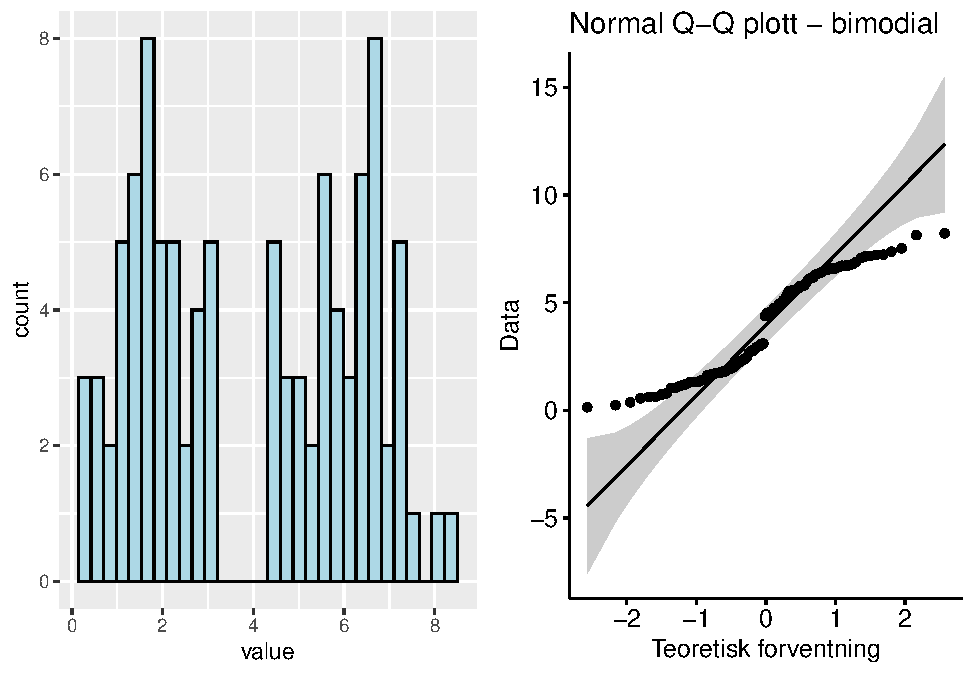
\includegraphics{02_Kap_2_files/figure-latex/unnamed-chunk-25-1.pdf}
\caption{\label{fig:unnamed-chunk-25}Q-Q plott - bimodal}
\end{figure}

Den bimodiale fordelingen viser ofte et brudd eller et distinkt knekkpunkt rundt krysning av den rette linja, med en del av linja på hver side av den rette linja.

\hypertarget{multimodalitet}{%
\subparagraph{Multimodalitet}\label{multimodalitet}}

\begin{Shaded}
\begin{Highlighting}[]
\CommentTok{\# Bruker pakken: readxl}
\CommentTok{\# Bruker pakken: tibble}
\NormalTok{qqmultimod }\OtherTok{\textless{}{-}} \FunctionTok{as\_tibble}\NormalTok{(}\FunctionTok{read\_xlsx}\NormalTok{(}\StringTok{"Multimodal.xlsx"}\NormalTok{))}
\CommentTok{\# Eksportere datasettet}
\CommentTok{\# Bruker pakken: writexl}
\FunctionTok{write\_xlsx}\NormalTok{(qqmultimod,}\StringTok{"QQ\_multimod.xlsx"}\NormalTok{)}
\end{Highlighting}
\end{Shaded}

\begin{Shaded}
\begin{Highlighting}[]
\CommentTok{\# Plotte histogram og Q{-}Q plott}
\CommentTok{\# Bruker pakken ggplot2}
\NormalTok{qqmultimodhist }\OtherTok{\textless{}{-}} \FunctionTok{ggplot}\NormalTok{(qqmultimod, }\FunctionTok{aes}\NormalTok{(}\AttributeTok{x=}\NormalTok{Verdi)) }\SpecialCharTok{+} \FunctionTok{geom\_histogram}\NormalTok{(}\AttributeTok{color=}\StringTok{"black"}\NormalTok{, }\AttributeTok{fill=}\StringTok{"lightblue"}\NormalTok{)}
\CommentTok{\# Bruker pakken: ggpubr}
\NormalTok{qqmultimod\_plott }\OtherTok{\textless{}{-}} \FunctionTok{ggqqplot}\NormalTok{(qqmultimod}\SpecialCharTok{$}\NormalTok{Verdi) }\SpecialCharTok{+} \FunctionTok{ggtitle}\NormalTok{(}\StringTok{"Normal Q{-}Q plott {-} multimodial"}\NormalTok{) }\SpecialCharTok{+} \FunctionTok{labs}\NormalTok{(}\AttributeTok{x =} \StringTok{"Teoretisk forventning"}\NormalTok{, }\AttributeTok{y =} \StringTok{"Data"}\NormalTok{)}
\CommentTok{\# Bruker pakken: gridExtra}
\FunctionTok{grid.arrange}\NormalTok{(qqmultimodhist, qqmultimod\_plott, }\AttributeTok{ncol=}\DecValTok{2}\NormalTok{)}
\end{Highlighting}
\end{Shaded}

\begin{figure}
\centering
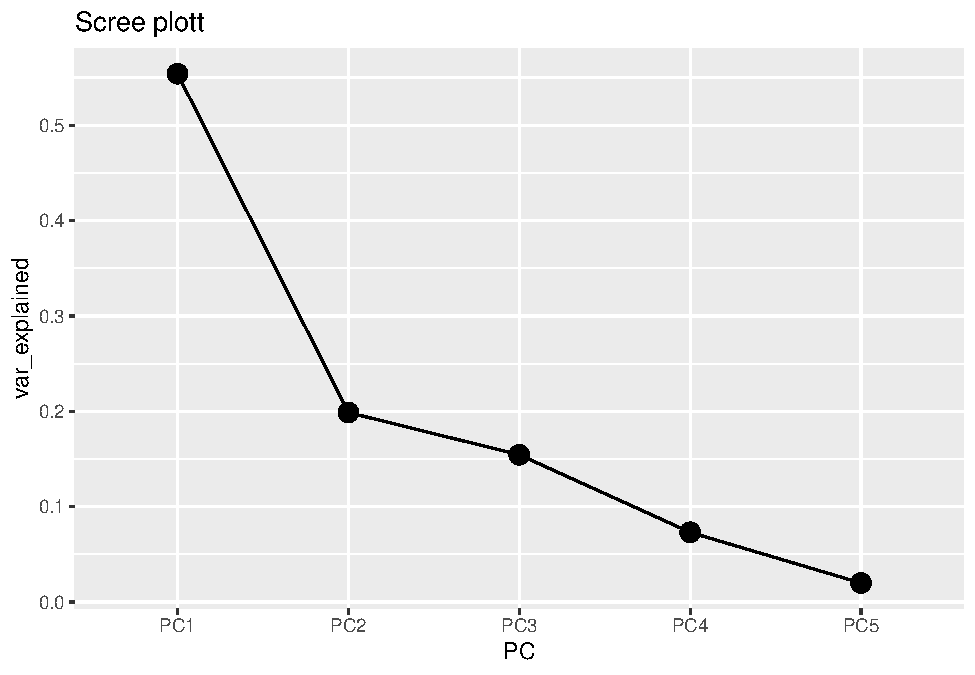
\includegraphics{02_Kap_2_files/figure-latex/unnamed-chunk-28-1.pdf}
\caption{\label{fig:unnamed-chunk-28}Q-Q plott - multimodal}
\end{figure}

Multimodale fordelinger vil som regel vise flere brudd.

\hypertarget{statistiske-tester-for-vurdering-av-dataenes-distribusjon}{%
\paragraph{Statistiske tester for vurdering av dataenes distribusjon}\label{statistiske-tester-for-vurdering-av-dataenes-distribusjon}}

Vi har nå sett på noen typiske eksempler på mønstre i Q-Q plott. Det kan imidlertid være vanskelig å bedømme fordelinger som ligger nære normalfordelingen, men likevel ikke perfekt oppå (du vil trolig aldri se en perfekt match med mindre du har generert et normalfordelt datasett med mange datapunkter). Vi kan supplere Q-Q plottene med visse statistiske tester (men husk: disse statistiske testene har sine egne forutsetninger og er heller ikke uten utfordringer).

\hypertarget{anderson-darling}{%
\subparagraph{Anderson-Darling}\label{anderson-darling}}

Anderson-Darlings test er en test for å se om et datasett kommer fra en gitt fordeling, f.eks. normalfordelingen \citep{andersonAsymptoticTheoryCertain1952b, andersonTestGoodnessFit1954}. Testen setter opp to hypoteser:

\begin{itemize}
\tightlist
\item
  \(H_0\): Dataene følger normalfordelingen
\item
  \(H_1\): Dataene følger ikke normalfordelingen
\end{itemize}

\begin{Shaded}
\begin{Highlighting}[]
\CommentTok{\# Bruker pakken: tibble}
\CommentTok{\# Bruker pakken: readxl}
\NormalTok{addata }\OtherTok{\textless{}{-}} \FunctionTok{as\_tibble}\NormalTok{(}\FunctionTok{read\_excel}\NormalTok{(}\StringTok{"Anderson{-}Darling\_raw.xlsx"}\NormalTok{))}
\CommentTok{\# Bruker pakken: nortest}
\FunctionTok{ad.test}\NormalTok{(addata}\SpecialCharTok{$}\NormalTok{Values)}
\CommentTok{\#\textgreater{} }
\CommentTok{\#\textgreater{}  Anderson{-}Darling normality test}
\CommentTok{\#\textgreater{} }
\CommentTok{\#\textgreater{} data:  addata$Values}
\CommentTok{\#\textgreater{} A = 0.74573, p{-}value = 0.04046}
\end{Highlighting}
\end{Shaded}

Siden vi vet at nullhypotesen er at datasettet \textbf{har} en normalfordeling vil vi forkaste nullhypotesen dersom vi har en signifikant p-verdi (grensen for hva som er signifikant bestemmer vi forsåvidt selv, men vanlige verdier er 0.01, 0.05 og 0.1). Altså - i dette tilfellet har vi en p-verdi=0.04. Vi forkaster derfor nullhypotesen og aksepterer \(H_1\) som sier at dataene er trolig ikke er normalfordelte (med andre ord: p-verdien må være større enn signifikansverdien for at vi skal si at dataene trolig er normalfordelte) - en huskeregel: ``If p is low, the null must go'' (her: ``low'' = under terskelverdien vi har satt, ofte 0.05).

Generisk ser dette slik ut \citep{hartmannELearningProjectSOGA2018}:

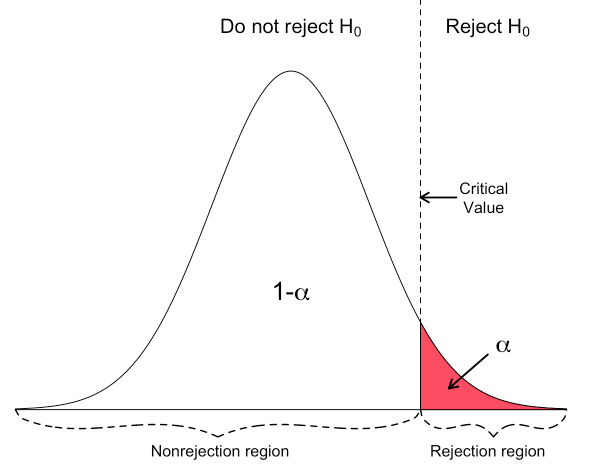
\includegraphics{Hartman1.png}

Det er verdt å merke seg at Anderson-Darling testen egentlig ikke forteller deg at dataene dine er normalfordelte, men at det er usannsynlig at de ikke er det om testen viser det. Dette synes kanskje som samme sak, men er i realiteten en viktig erkjennelse -- en tørr gressplen er et bevis for at det ikke har regnet, men en våt gressplen er ikke bevis for at det har regnet. En våt gressplen kan skyldes andre ting enn regn. Altså -- en signifikant p-verdi på testen gjør at vi forkaster \(H_0\) og antar at fordelingen er ikke-normal. En ikke-signifikant p-verdi på gjør at vi med f.eks. 95\% konfidens kan si at vi ikke har funnet avvik fra normalfordelingen.

Tabellarisk kan vi oppsummere vurderingene slik:

\begin{table}[!h]
\centering
\begin{tabular}{l|l}
\hline
Betingelse & Vurdering\\
\hline
p-verdi $\le$ valgt signifikansnivå & Forkast $H_0$ - datene er trolig ikke normalfordelte\\
\hline
p-verdi > valgt signifikansnivå & Behold $H_0$ - dataene er trolig normalfordelte\\
\hline
Testverdi ($A^2$ verdi) > kritisk verdi & Forkast $H_0$ - datene er trolig ikke normalfordelte\\
\hline
Testverdi ($A^2$ verdi) $\le$ kritisk verdi & Behold $H_0$ - dataene er trolig normalfordelte\\
\hline
\end{tabular}
\end{table}

Det finnes flere andre statistiske tester som kan kjøres for å teste for normalitet, f.eks. Kolmogorov-Smirnov, Shapiro-Wilks og Cramer Von-Mises test. Anderson-Darling er en modifisering/videreutvikling av Kolmogorov-Smirnov og anses ofte som en bedre test av de to. Andre kilder (se f.eks. \citet{razaliPowerComparisonsShapiroWilk2011}) finner at Shapiro-Wilks presterer best i 10 000 simuleringer på ulike distribusjoner.

\begin{Shaded}
\begin{Highlighting}[]
\FunctionTok{options}\NormalTok{(}\AttributeTok{scipen=}\DecValTok{999}\NormalTok{)}
\CommentTok{\# Bruker pakken: tibble}
\CommentTok{\# Bruker pakken: readxl}
\NormalTok{addata5 }\OtherTok{\textless{}{-}} \FunctionTok{as\_tibble}\NormalTok{(}\FunctionTok{read\_excel}\NormalTok{(}\StringTok{"Anderson{-}Darling\_raw.xlsx"}\NormalTok{))}
\CommentTok{\# Base R}
\FunctionTok{ks.test}\NormalTok{(addata5, }\StringTok{"pnorm"}\NormalTok{)}
\CommentTok{\#\textgreater{} }
\CommentTok{\#\textgreater{}  One{-}sample Kolmogorov{-}Smirnov test}
\CommentTok{\#\textgreater{} }
\CommentTok{\#\textgreater{} data:  addata5}
\CommentTok{\#\textgreater{} D = 0.88493, p{-}value = 0.0000000000000171}
\CommentTok{\#\textgreater{} alternative hypothesis: two{-}sided}
\end{Highlighting}
\end{Shaded}

\begin{Shaded}
\begin{Highlighting}[]
\CommentTok{\# Base R}
\FunctionTok{shapiro.test}\NormalTok{(addata5}\SpecialCharTok{$}\NormalTok{Values)}
\CommentTok{\#\textgreater{} }
\CommentTok{\#\textgreater{}  Shapiro{-}Wilk normality test}
\CommentTok{\#\textgreater{} }
\CommentTok{\#\textgreater{} data:  addata5$Values}
\CommentTok{\#\textgreater{} W = 0.87521, p{-}value = 0.04027}
\end{Highlighting}
\end{Shaded}

\begin{Shaded}
\begin{Highlighting}[]
\CommentTok{\# bruker pakken: nortest}
\FunctionTok{cvm.test}\NormalTok{(addata}\SpecialCharTok{$}\NormalTok{Values)}
\CommentTok{\#\textgreater{} }
\CommentTok{\#\textgreater{}  Cramer{-}von Mises normality test}
\CommentTok{\#\textgreater{} }
\CommentTok{\#\textgreater{} data:  addata$Values}
\CommentTok{\#\textgreater{} W = 0.12634, p{-}value = 0.04326}
\end{Highlighting}
\end{Shaded}

Tolkning Kolmogorov-Smirnov: Hvis p-verdien er under valgte signifikansnivå (f.eks. 0.05) skal vi anta at datasettet ikke er normalfordelt. Her vil testen peke på at datasettet \emph{ikke} er normalfordelt.

Tolkning av Shapiro-Wilks og Cramer-von Mieses test er lik som for Kolmogorov-Smirnov.

Som et siste eksempel på en statistisk test for normalitet kan vi bruke Jarque-Bera test. Denne skiller seg litt ut fra de andre ved at den spesifikt ser på skjevhet og kurtosis i datasettet opp mot hva en normalfordeling vil ha. For å gjøre lykken komplett finnes det versjoner av testen:

\begin{Shaded}
\begin{Highlighting}[]
\CommentTok{\# Bruker pakken: tibble}
\CommentTok{\# bruker pakken: readxl}
\NormalTok{addata6 }\OtherTok{\textless{}{-}} \FunctionTok{as\_tibble}\NormalTok{(}\FunctionTok{read\_excel}\NormalTok{(}\StringTok{"Anderson{-}Darling\_raw.xlsx"}\NormalTok{))}
\CommentTok{\# Bruker pakken: tseries}
\FunctionTok{jarque.bera.test}\NormalTok{(addata6}\SpecialCharTok{$}\NormalTok{Values)}
\CommentTok{\#\textgreater{} }
\CommentTok{\#\textgreater{}  Jarque Bera Test}
\CommentTok{\#\textgreater{} }
\CommentTok{\#\textgreater{} data:  addata6$Values}
\CommentTok{\#\textgreater{} X{-}squared = 2.1953, df = 2, p{-}value = 0.3337}
\end{Highlighting}
\end{Shaded}

\begin{Shaded}
\begin{Highlighting}[]
\CommentTok{\# Bruker pakken: normtest}
\FunctionTok{ajb.norm.test}\NormalTok{(addata6}\SpecialCharTok{$}\NormalTok{Values, }\AttributeTok{nrepl=}\DecValTok{2000}\NormalTok{)}
\CommentTok{\#\textgreater{} }
\CommentTok{\#\textgreater{}  Adjusted Jarque{-}Bera test for normality}
\CommentTok{\#\textgreater{} }
\CommentTok{\#\textgreater{} data:  addata6$Values}
\CommentTok{\#\textgreater{} AJB = 3.1014, p{-}value = 0.131}
\end{Highlighting}
\end{Shaded}

Tolkningen er lik som før - hvis p-verdien er mindre enn valgte signifikansnivå peker det mot at datasettet ikke er normalfordelt. Her, i motsetning til de øvrige testene, er p-verdien større enn signifikansnivået (0,05) så det peker mot at datasettet \emph{er} normalfordelt.

Dette er altså ikke så enkelt. Det finnes mange statistiske tester, som kan gi motsatte indikasjoner på om et datasett er normalfordelt eller ikke siden de ser på dataene fra ``ulik vinkel'' (fokuserer på ulike aspekter ved dataene). \textbf{Vårt råd blir:} Start alltid med Q-Q plott. Velg evt en teststatistikk, men vær klar over at alle teststatistikker bygger på forutsetninger eller tester ulike sider av distribusjonen. Det vi også kan huske på er at i henhold til sentralgrenseteoremet (``Central Limit Theorem'') vil populasjonens fordeling være av mindre interesse dersom utvalgsstørrelsen er stor nok. Hva er stor nok? De fleste kilder peker mot at over 30 er ``stort nok''.

\hypertarget{boxplott}{%
\paragraph{Boxplott}\label{boxplott}}

\begin{Shaded}
\begin{Highlighting}[]
\CommentTok{\# Base R}
\FunctionTok{par}\NormalTok{(}\AttributeTok{mfrow=}\NormalTok{(}\FunctionTok{c}\NormalTok{(}\DecValTok{1}\NormalTok{,}\DecValTok{2}\NormalTok{)))}
\FunctionTok{Boxplot}\NormalTok{(Field\_OLS\_data}\SpecialCharTok{$}\NormalTok{Adverts, }\AttributeTok{id =} \FunctionTok{list}\NormalTok{(}\AttributeTok{n=}\ConstantTok{Inf}\NormalTok{), }\AttributeTok{ylab =} \StringTok{""}\NormalTok{, }\AttributeTok{main =} \StringTok{"Adverts"}\NormalTok{, }\AttributeTok{col =} \StringTok{"Blue"}\NormalTok{)}
\CommentTok{\#\textgreater{} [1]  43  87 184}
\FunctionTok{Boxplot}\NormalTok{(Field\_OLS\_data}\SpecialCharTok{$}\NormalTok{Sales, }\AttributeTok{id =} \FunctionTok{list}\NormalTok{(}\AttributeTok{n=}\ConstantTok{Inf}\NormalTok{), }\AttributeTok{ylab =} \StringTok{""}\NormalTok{, }\AttributeTok{main =} \StringTok{"Sales"}\NormalTok{, }\AttributeTok{col =} \StringTok{"Green"}\NormalTok{)}
\end{Highlighting}
\end{Shaded}

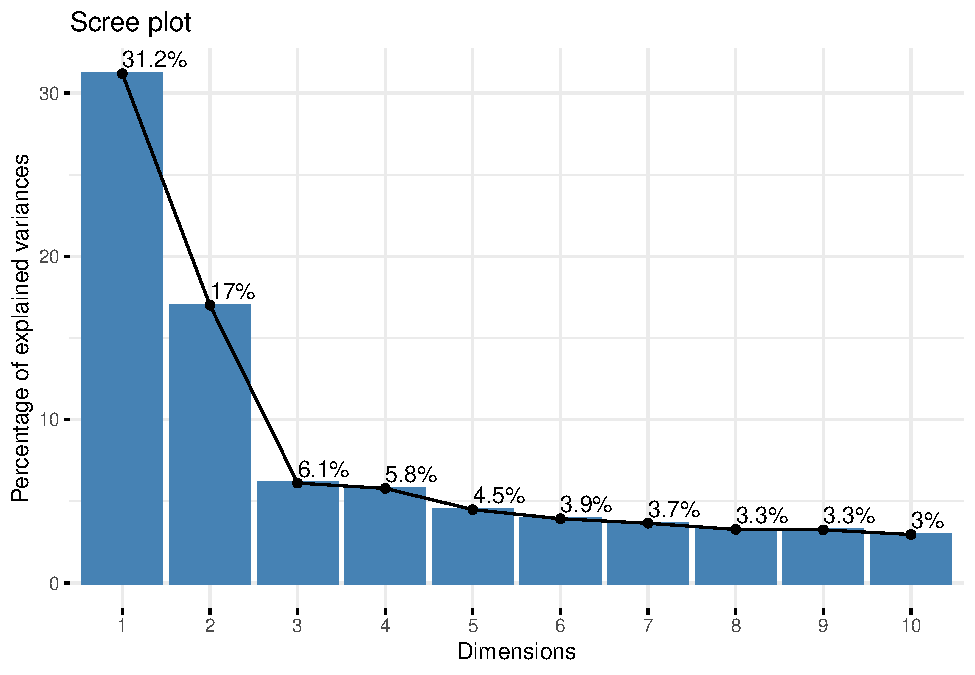
\includegraphics{02_Kap_2_files/figure-latex/unnamed-chunk-37-1.pdf}
Vi ser at vi får først ut en liste over uteliggerne identifisert ved id/case/observasjonsnummer (43, 87 og 184) for variabelen Adverts. Dette vises også som tre små sirkler i boxplottet.

Et boxplott forteller oss mye om dataenes distribusjon.

\begin{itemize}
\tightlist
\item
  Selve boksen representerer 50 \% av observasjonene/casene, det vil si at nedre kant representerer første kvartil (= 25.prosentil) og øvre kant tredje kvartil (= 75.prosentil).
\item
  Den tykkere horisontale streken i boksen viser medianverdien (= andre kvartil = 50.prosentil)
\item
  Dersom en observasjon ligger utenfor en terkselverdi (jfr figur under) vises dette med en liten sirkel. Dette defineres som uteliggere. Å identifisere uteliggere kan være viktig for mange statistiske tester.
\end{itemize}

\citet{galarnykUnderstandingBoxplots2018} illustrerer boxplott slik:

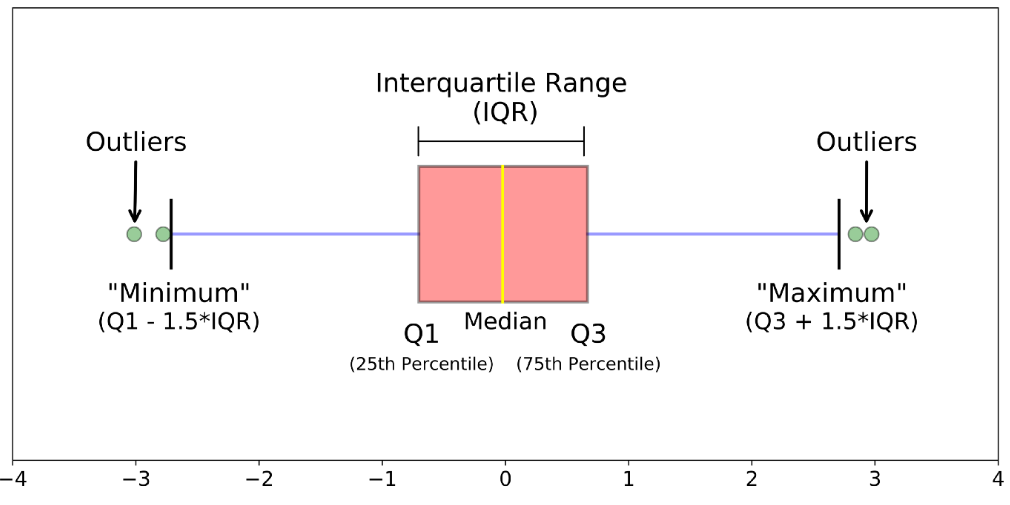
\includegraphics[width=0.5\textwidth,height=\textheight]{Boxplott.png}

\hypertarget{scatterplott}{%
\paragraph{Scatterplott}\label{scatterplott}}

\begin{Shaded}
\begin{Highlighting}[]
\CommentTok{\# Bruker pakken: ggplot2}
\FunctionTok{ggplot}\NormalTok{(Field\_OLS\_data, }\FunctionTok{aes}\NormalTok{(}\AttributeTok{x =}\NormalTok{ Adverts, }\AttributeTok{y =}\NormalTok{ Sales)) }\SpecialCharTok{+}
  \FunctionTok{geom\_point}\NormalTok{(}\AttributeTok{colour =} \DecValTok{4}\NormalTok{)}
\end{Highlighting}
\end{Shaded}

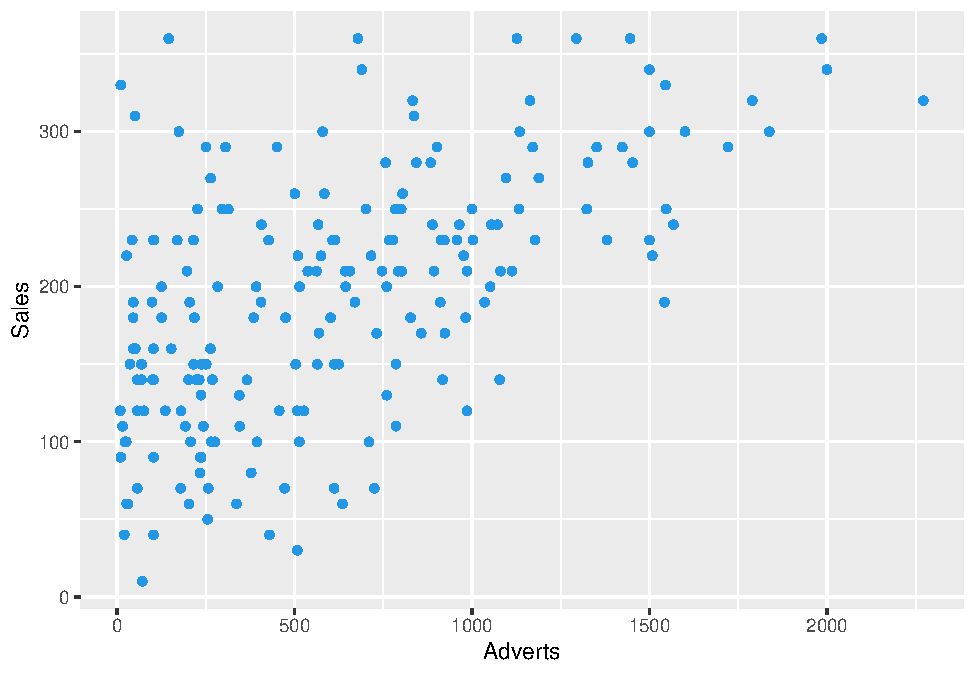
\includegraphics{02_Kap_2_files/figure-latex/unnamed-chunk-38-1.pdf}

Et scatterplott viser oss på en god visuell måte hvordan de to variablene forholder seg til hverandre (vi plotter hver enkelt observasjon gjennom verdiene de har på de to variablene). Mønsteret kan derfor si oss mye om sammenhengen mellom de to.

En god måte å fremstille et scatterplott på i R (gjennom pakken \emph{car}) er denne:

\begin{Shaded}
\begin{Highlighting}[]
\CommentTok{\# Bruker pakken: car}
\FunctionTok{scatterplot}\NormalTok{(Adverts }\SpecialCharTok{\textasciitilde{}}\NormalTok{ Sales, }\AttributeTok{data =}\NormalTok{ Field\_OLS\_data, }\AttributeTok{id =} \FunctionTok{list}\NormalTok{(}\AttributeTok{n=}\DecValTok{4}\NormalTok{))}
\end{Highlighting}
\end{Shaded}

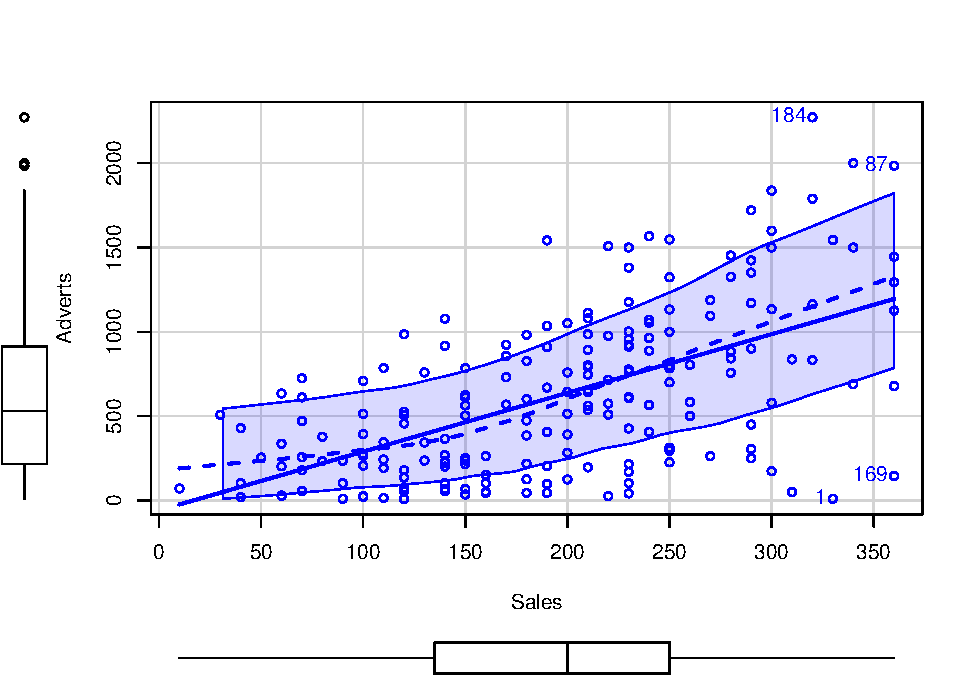
\includegraphics{02_Kap_2_files/figure-latex/unnamed-chunk-39-1.pdf}

\begin{verbatim}
#> [1]   1  87 169 184
\end{verbatim}

Her kombinerer vi scatterplott og boxplott. Den rette blå linja er en minste kvadratssums regresjonslinje (OLS). Den stiplede blå linja bruker en ikke-parametrisk tilnærming. I tillegg får vi visualisert de fire mest ekstreme tilfellene (lengst vekk fra gjennomsnitt).

\hypertarget{steg-2-evtentuelt-valg-av-prediktorer-ut-fra-analyse-av-dataene}{%
\subsubsection{Steg 2: Evtentuelt valg av prediktorer ut fra analyse av dataene}\label{steg-2-evtentuelt-valg-av-prediktorer-ut-fra-analyse-av-dataene}}

Dette er ikke relevant i en enkel lineær regresjonsanalyse. Når vi skal gjøre en multippel regresjonsanalyse - altså at vi har to eller flere uavhengige variabler (prediktorer) vil analysen av dataene våre - og i hvilken rekkefølge vi legger de uavhengige variablene inn i regresjonsmodellen (mer om det under eksempelet for multippel regresjon) kunne informeres av analysen vi gjør i forkant. Derfor viser vi dette nå selv om det altså ikke er relevant for enkel regresjonsanalyse.

Vi lager en korrelasjonstabell for de tre uavhengige og den avhengige variabelen (Sales, Adverts, Airplay, Image):

\begin{Shaded}
\begin{Highlighting}[]
\CommentTok{\# Bruker pakken: sjPlot}
\FunctionTok{tab\_corr}\NormalTok{(Field\_OLS\_data, }\AttributeTok{triangle =} \StringTok{"lower"}\NormalTok{)}
\end{Highlighting}
\end{Shaded}

~

Adverts

Sales

Airplay

Image

Adverts

~

~

~

~

Sales

0.578***

~

~

~

Airplay

0.102{}

0.599***

~

~

Image

0.081{}

0.326***

0.182**

~

Computed correlation used pearson-method with listwise-deletion.

p \textless{} .0001**** , p \textless{} .001*** , p \textless{} .01**, p \textless{} .05*

I standard multippel regresjonsanalyse legger vi alle de uavhengige variablene inn samtidig. Dersom vi skal gjøre en stegvis regresjonsanalyse vil vi legge de uavhengige variablene inn en og en ut fra statistiske kriterier - som hvor stor korrelasjonen er. Den uavhengige variabelen med størst korrelasjon legges inn først og så videre. For det eksempelet vi har ser vi at Sales korrelerer høyest med Airplay, og nesten like mye med Adverts. Korrelasjonen med Image er noe lavere.

\hypertarget{steg-3-lage-modell-og-kjuxf8re-regresjonsanalysen}{%
\subsubsection{Steg 3: Lage modell (og kjøre regresjonsanalysen)}\label{steg-3-lage-modell-og-kjuxf8re-regresjonsanalysen}}

Vi ønsker å se om Adverts kan predikere Sales. Grafisk kan vi vise dette:

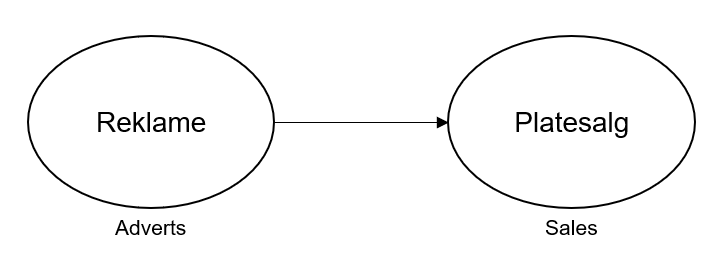
\includegraphics[width=0.5\textwidth,height=\textheight]{OLS1.png}

\begin{Shaded}
\begin{Highlighting}[]
\CommentTok{\# Bruker pakken: olsrr}
\NormalTok{FieldOLS\_reg }\OtherTok{\textless{}{-}} \FunctionTok{ols\_regress}\NormalTok{(Sales }\SpecialCharTok{\textasciitilde{}}\NormalTok{ Adverts, }\AttributeTok{data =}\NormalTok{ Field\_OLS\_data)}
\end{Highlighting}
\end{Shaded}

\hypertarget{steg-4-analyse-av-resultatene-diagnostikk}{%
\subsubsection{Steg 4: Analyse av resultatene (diagnostikk)}\label{steg-4-analyse-av-resultatene-diagnostikk}}

\begin{Shaded}
\begin{Highlighting}[]
\CommentTok{\# Bruker pakken: olsrr}
\NormalTok{FieldOLS\_reg}
\CommentTok{\#\textgreater{}                          Model Summary                           }
\CommentTok{\#\textgreater{} {-}{-}{-}{-}{-}{-}{-}{-}{-}{-}{-}{-}{-}{-}{-}{-}{-}{-}{-}{-}{-}{-}{-}{-}{-}{-}{-}{-}{-}{-}{-}{-}{-}{-}{-}{-}{-}{-}{-}{-}{-}{-}{-}{-}{-}{-}{-}{-}{-}{-}{-}{-}{-}{-}{-}{-}{-}{-}{-}{-}{-}{-}{-}{-}}
\CommentTok{\#\textgreater{} R                       0.578       RMSE                 65.991 }
\CommentTok{\#\textgreater{} R{-}Squared               0.335       Coef. Var            34.157 }
\CommentTok{\#\textgreater{} Adj. R{-}Squared          0.331       MSE                4354.870 }
\CommentTok{\#\textgreater{} Pred R{-}Squared          0.323       MAE                  50.869 }
\CommentTok{\#\textgreater{} {-}{-}{-}{-}{-}{-}{-}{-}{-}{-}{-}{-}{-}{-}{-}{-}{-}{-}{-}{-}{-}{-}{-}{-}{-}{-}{-}{-}{-}{-}{-}{-}{-}{-}{-}{-}{-}{-}{-}{-}{-}{-}{-}{-}{-}{-}{-}{-}{-}{-}{-}{-}{-}{-}{-}{-}{-}{-}{-}{-}{-}{-}{-}{-}}
\CommentTok{\#\textgreater{}  RMSE: Root Mean Square Error }
\CommentTok{\#\textgreater{}  MSE: Mean Square Error }
\CommentTok{\#\textgreater{}  MAE: Mean Absolute Error }
\CommentTok{\#\textgreater{} }
\CommentTok{\#\textgreater{}                                  ANOVA                                   }
\CommentTok{\#\textgreater{} {-}{-}{-}{-}{-}{-}{-}{-}{-}{-}{-}{-}{-}{-}{-}{-}{-}{-}{-}{-}{-}{-}{-}{-}{-}{-}{-}{-}{-}{-}{-}{-}{-}{-}{-}{-}{-}{-}{-}{-}{-}{-}{-}{-}{-}{-}{-}{-}{-}{-}{-}{-}{-}{-}{-}{-}{-}{-}{-}{-}{-}{-}{-}{-}{-}{-}{-}{-}{-}{-}{-}{-}}
\CommentTok{\#\textgreater{}                    Sum of                                               }
\CommentTok{\#\textgreater{}                   Squares         DF    Mean Square      F         Sig. }
\CommentTok{\#\textgreater{} {-}{-}{-}{-}{-}{-}{-}{-}{-}{-}{-}{-}{-}{-}{-}{-}{-}{-}{-}{-}{-}{-}{-}{-}{-}{-}{-}{-}{-}{-}{-}{-}{-}{-}{-}{-}{-}{-}{-}{-}{-}{-}{-}{-}{-}{-}{-}{-}{-}{-}{-}{-}{-}{-}{-}{-}{-}{-}{-}{-}{-}{-}{-}{-}{-}{-}{-}{-}{-}{-}{-}{-}}
\CommentTok{\#\textgreater{} Regression     433687.833          1     433687.833    99.587    0.0000 }
\CommentTok{\#\textgreater{} Residual       862264.167        198       4354.870                     }
\CommentTok{\#\textgreater{} Total         1295952.000        199                                    }
\CommentTok{\#\textgreater{} {-}{-}{-}{-}{-}{-}{-}{-}{-}{-}{-}{-}{-}{-}{-}{-}{-}{-}{-}{-}{-}{-}{-}{-}{-}{-}{-}{-}{-}{-}{-}{-}{-}{-}{-}{-}{-}{-}{-}{-}{-}{-}{-}{-}{-}{-}{-}{-}{-}{-}{-}{-}{-}{-}{-}{-}{-}{-}{-}{-}{-}{-}{-}{-}{-}{-}{-}{-}{-}{-}{-}{-}}
\CommentTok{\#\textgreater{} }
\CommentTok{\#\textgreater{}                                     Parameter Estimates                                     }
\CommentTok{\#\textgreater{} {-}{-}{-}{-}{-}{-}{-}{-}{-}{-}{-}{-}{-}{-}{-}{-}{-}{-}{-}{-}{-}{-}{-}{-}{-}{-}{-}{-}{-}{-}{-}{-}{-}{-}{-}{-}{-}{-}{-}{-}{-}{-}{-}{-}{-}{-}{-}{-}{-}{-}{-}{-}{-}{-}{-}{-}{-}{-}{-}{-}{-}{-}{-}{-}{-}{-}{-}{-}{-}{-}{-}{-}{-}{-}{-}{-}{-}{-}{-}{-}{-}{-}{-}{-}{-}{-}{-}{-}{-}{-}{-}}
\CommentTok{\#\textgreater{}       model       Beta    Std. Error    Std. Beta      t        Sig       lower      upper }
\CommentTok{\#\textgreater{} {-}{-}{-}{-}{-}{-}{-}{-}{-}{-}{-}{-}{-}{-}{-}{-}{-}{-}{-}{-}{-}{-}{-}{-}{-}{-}{-}{-}{-}{-}{-}{-}{-}{-}{-}{-}{-}{-}{-}{-}{-}{-}{-}{-}{-}{-}{-}{-}{-}{-}{-}{-}{-}{-}{-}{-}{-}{-}{-}{-}{-}{-}{-}{-}{-}{-}{-}{-}{-}{-}{-}{-}{-}{-}{-}{-}{-}{-}{-}{-}{-}{-}{-}{-}{-}{-}{-}{-}{-}{-}{-}}
\CommentTok{\#\textgreater{} (Intercept)    134.140         7.537                 17.799    0.000    119.278    149.002 }
\CommentTok{\#\textgreater{}     Adverts      0.096         0.010        0.578     9.979    0.000      0.077      0.115 }
\CommentTok{\#\textgreater{} {-}{-}{-}{-}{-}{-}{-}{-}{-}{-}{-}{-}{-}{-}{-}{-}{-}{-}{-}{-}{-}{-}{-}{-}{-}{-}{-}{-}{-}{-}{-}{-}{-}{-}{-}{-}{-}{-}{-}{-}{-}{-}{-}{-}{-}{-}{-}{-}{-}{-}{-}{-}{-}{-}{-}{-}{-}{-}{-}{-}{-}{-}{-}{-}{-}{-}{-}{-}{-}{-}{-}{-}{-}{-}{-}{-}{-}{-}{-}{-}{-}{-}{-}{-}{-}{-}{-}{-}{-}{-}{-}}
\end{Highlighting}
\end{Shaded}

\hypertarget{hvor-mye-forklarer-modellen-vuxe5r}{%
\paragraph{Hvor mye forklarer modellen vår?}\label{hvor-mye-forklarer-modellen-vuxe5r}}

Det første vi kan se på er \(R^{2}\) som forteller oss hvor stor del av den totale variansen modellen forklarer. I dette tilfellet er \(R^{2} = 0.3346\). Det innebærer at modellen vår kan forklare 33.46 \% av den totale variansen. Det betyr at reklame forklarer («accounts for») 33.5 \% av variansen i salget. Det er med andre ord mange andre faktorer som kan forklare hvorfor noen plater selger bedre enn andre, men reklame kan forklare drøye 33 \% av den totale variansen. Dette kan vi også se er statistisk signifikant p \textless{} .001.

Endel programmer vil også gi en R verdi. Siden vi kun har en uavhengig variabel (en prediktor) vil verdien R utgjøre den bivariate korrelasjonen (korrelasjonskoeffisienten mellom de to variablene - vi ser at dette er samme verdi som i tabellen over korrelasjonskoeffisienter lenger opp).

Adjusted \(R^{2}\) er en ``modifisert versjon'' av \(R^{2}\) der det legges inn en korreksjon for antall prediktorer i modellen. Motivasjonen for dette er at det å legge til flere prodeiktorer \emph{alltid} vil øke \(R^{2}\) verdien \citep{navarroLearningStatisticsJamovi2019a}. \citet{navarroLearningStatisticsJamovi2019a} påpeker imidlertid at man ikke kan tolke adjusted \(R^{2}\) like rett fram som \(R^{2}\), og anbefaler at man bruker \(R^{2}\). Det vi også kan si er at dersom verdiene på henholdsvis \(R^{2}\) og adjusted \(R^{2}\) er nærme hverandre (eller like) indikerer dette en god kryssvaliditet i modellen, noe som kan gjøre oss sikrere i generalisering av funnene våre.

\hypertarget{modellens-koeffisienter-og-regresjonslikning}{%
\paragraph{Modellens koeffisienter og regresjonslikning}\label{modellens-koeffisienter-og-regresjonslikning}}

Koeffisientene vil fortelle oss mer i multippel regresjonsanalyse, men gir oss noen interessante opplysninger også her. I introduksjonen snakket vi om punktet der regresjonslinja skjærer y-aksen (konstanten). Fra analysen ser vi at (Intercept) = 134.14 og Adverts = 0.096. 134.14 er punktet på y-aksen regresjonslinja ``begynner'' (der x = 0). Altså, ettersom x-aksen angir verdier for hva vi bruker på reklame er Intercept estimatet antallet plater vi kan forvente å selge dersom vi bruker 0 kroner på reklame. Estimatet på «Adverts» på 0,096 er stigningstallet for regresjonslinja -- hvis prediktoren (reklame) stiger med 1 enhet stiger salget med 0,096 plater. Vi kan da lage følgende likning: \[ Sales=134,14\:+\:0,096\left(Adverts\right) \]

\hypertarget{hvor-god-er-modellen-vuxe5r-goodness-of-fit}{%
\paragraph{Hvor god er modellen vår (goodness of fit)?}\label{hvor-god-er-modellen-vuxe5r-goodness-of-fit}}

Vi ønsker å ha en formening om hvor god modellen er («goodness of fit»). Altså, er regresjonsmodellen vår bedre enn en modell der vi ikke vet noe om forholdet mellom reklame og platesalg? Vi kan bruke gjennomsnitt av salgstallene som en modell for ingen sammenheng mellom reklame og platesalg, og deretter sammenlikne regresjonsmodellen med gjennomsnittsmodellen. Sammenlikningen mellom modellene skjer gjennom å se på forskjellene mellom de observerte målingene (salgstall) og verdier predikert at de to ulike modellene. Dersom regresjonsmodellen signifikant predikerer bedre er det en bedre modell enn alternativet.

Analysen vår har gitt oss F verdien 99.59 med p \textless{} .001. Vi ser at verdien er statistisk signifikant. F verdien er et mål på forbedring i prediksjonen sett opp mot unøyaktigheter i modellen (alle modeller er unøyaktige (eller ``feil'')).
Vi kan sjekke F-verdien opp mot antall frihetsgrader (df) gjennom tabeller som ofte finnes i statistikkbøker, eller bruke onlineressurser som \href{http://www.stat.purdue.edu/~jtroisi/STAT350Spring2015/tables/FTable.pdf}{her}

Vi ser av resultatene fra analysen at antall df i teller er 1 og antall df i nevner er 198. Hvis vi leser av tabellen ser vi at for df 1/df 200 er kritisk verdi 3,89 for α = 0,05 og 11,15 for α = 0,001. Vår F er med andre ord langt over kritisk verdi. Vi kan derfor si at vår regresjonsmodell gir en signifikant bedre prediksjon av platesalg enn alternativet. Reklame er med andre ord en god prediktor for platesalg.

Helt nøyaktig kan vi regne ut kritisk verdi (som vi har gjort i R) for df 1 og df 198:

\begin{Shaded}
\begin{Highlighting}[]
\CommentTok{\# Base R}
\FunctionTok{qf}\NormalTok{(}\AttributeTok{p=}\NormalTok{.}\DecValTok{05}\NormalTok{, }\AttributeTok{df1=}\DecValTok{1}\NormalTok{, }\AttributeTok{df2=}\DecValTok{198}\NormalTok{, }\AttributeTok{lower.tail=}\ConstantTok{FALSE}\NormalTok{)}
\CommentTok{\#\textgreater{} [1] 3.888853}
\end{Highlighting}
\end{Shaded}

Ut fra dette kan vi si det er svært usannsynlig at forbedringen fra referansemodellen (gjennomsnittet) til vår modell er tilfeldig. Vi kan også si at dersom forbedringen ved regresjonsmodellen er større enn unøyaktigheten i modellen så vil F \textgreater{} 1.

Til slutt vil vi se på konfidensintervallet:

\begin{Shaded}
\begin{Highlighting}[]
\CommentTok{\# Bruker pakken: car}
\NormalTok{FieldOLS\_reg }\OtherTok{\textless{}{-}} \FunctionTok{lm}\NormalTok{(Sales }\SpecialCharTok{\textasciitilde{}}\NormalTok{ Adverts, Field\_OLS\_data)}
\FunctionTok{Confint}\NormalTok{(FieldOLS\_reg)}
\CommentTok{\#\textgreater{}                 Estimate        2.5 \%      97.5 \%}
\CommentTok{\#\textgreater{} (Intercept) 134.13993781 119.27768082 149.0021948}
\CommentTok{\#\textgreater{} Adverts       0.09612449   0.07712929   0.1151197}
\end{Highlighting}
\end{Shaded}

\hypertarget{steg-5-sjekk-av-forutsetningene}{%
\subsubsection{Steg 5: Sjekk av forutsetningene}\label{steg-5-sjekk-av-forutsetningene}}

Dette er et tema som behandles og framstilles på noe ulike måter i litteraturen. Det som er klart er at brudd på forutsetningene \emph{kan} gjøre modellen vår mer usikker opp til et punkt hvor regresjonsanalyse ikke bør gjennomføres. Noen av forutsetningene er empirisk testbare (vi kan få ut en eller annen form for analyse av et statistikkprogram som SPSS, Stata, R og så videre) mens noen er ikke empirisk testbare (det vil si vi må bruke egen vurdering). Vi skal i dette delkapittelet gå gjennom forutsetningene for lineær regresjon. Selv om noen ikke er aktuelle for enkel regresjon tar vi med alle forutsetningene her for oversiktens skyld.

Ved regresjonsanalyse gjør vi en rekke sjekker av datamaterialet vi har for å avgjøre om regresjonsanalyse er en egnet teknikk og hvorvidt vi mener vi kan generalisere funnene. Dersom forutsetningene brytes gjør det at vi kan sette spørsmålstegn ved hvor nærme regresjonskoeffisienten er populasjonskoeffisienten -- eller med andre ord: Hvis regresjonskoeffisienten er helt forventningsrett («unbiased», dvs 0) så vil regresjonskoeffisienten være lik populasjonskoeffisienten («estimatet er lik virkeligheten»). Nå vil det i praksis aldri være tilfelle, men ved å sette visse forutsetninger kan vi fastslå om våre data egner seg for regresjonsanalyse og hvor sikre vi føler oss for at funnene kan generaliseres. Det er verdt å merke seg hva Field et. al \citeyearpar[s.298]{fieldDiscoveringStatisticsUsing2012} skriver:

\begin{quote}
``It's worth remembering that you can have a perfectly good model for your data (no outliers, influential cases, etc.) and you can use that model to draw conclusions about your sample, even if your assumptions are violated. However, it's much more interesting to generalize your regression model and this is where assumptions become important. If they have been violated then you cannot generalize your findings beyond your sample.''
\end{quote}

Med andre ord: Vi kan ha brudd på forutsetningene og likevel si noe meningsfullt om vårt utvalg/våre data, men resultatene våre blir mer usikre og vi skal være veldig forsiktige med å kreve generaliserbarhet dersom vi har brudd på forutsetningene. Så alt håp er ikke ute med brudd på forutsetningene, men vi skal behandle konklusjonene våre deretter.

Regresjonsforutsetninger behandles ulikt av ulke kilder, og får ulik plass i diskusjoner om regresjon. Vi har undersøkt en rekke kilder for å framstille dette her (blant annet \citet{greenHowManySubjects1991}, \citet{berryUnderstandingRegressionAssumptions1993}, \citet{milesApplyingRegressionCorrelation2001}, \citet{hinkleAppliedStatisticsBehavioral2003}, \citet{tabachnikUsingMultivariateStatistics2007}, \citet{eikemoKvantitativAnalyseMed2007}, \citet{hairjr.MultivariateDataAnalysis2010}, \citet{lomaxStatisticalConceptsSecond2012}).

\hypertarget{kausalitet}{%
\paragraph{Kausalitet}\label{kausalitet}}

Forutsetningen om kausalitet hviler i fagunnskap og teoretiske vurderinger. Det sier seg for så vidt selv at vi ikke er interesserte i å ha med irrelevante variabler i modellen. Med irrelevant her menes variabler som korrelerer med den avhengige variabelen, men hvor korrelasjonen er ikke har noe med årsakssammenheng å gjøre (sammenhenger medfører ikke i seg selv kausalitet som vi har vært inne på i en tidligere modul).

Kausalitet er dermed en forutsetning. Den uavhengige variabelen må variere korrelert med de avhengige, det er en kausal sammenheng (hvis ikke det er kausalitet har den/de uavhengige variablene ingen effekt på den avhengige -- det kan like gjerne være motsatt). Når vi velger en avhengig variabel og en eller flere uavhengige variabler har vi også gjort en antakelse om kausalitet og retning på kausaliteten, og forutsatt at denne er tilstede - basert på teoretisk kunnskap om det vi undersøker. Men det er viktig å understreke at verken korrelasjon eller regresjon indikerer kausalitet.

\hypertarget{variablene-er-uten-muxe5lefeil}{%
\paragraph{Variablene er uten målefeil}\label{variablene-er-uten-muxe5lefeil}}

Vi må forutsette at vi ikke har systematiske målefeil i våre data. \citet{thoresenMalefeilRegresjonsanalyse2003} viser for eksempel til en studie av \citet{macmahonBloodPressureStroke1990} der de fant en 60\% sterkere sammneheng mellom blodtrykk og hjerte-karsykdommer i en stor metastudie når de korrigerte for skjevhet i estimatene i de tidligere studiene (som var inkludert i metastudien).

Vi skal også være oppmerksom på utfordringer dersom feil i den ene variabelen korrelerer med feil i en annen variabel. ``Dersom målt eksponering og målt helseutfall er rammet av avhengige feil, blir resultatet oftest en falskt forhøyet sammenheng mellom de to. Slik resultatskjevhet er sannsynligvis ikke uvanlig i tverrsnittsstudier, hvor data om eksponering og utfall skaffes til veie gjennom spørreskjema'' \citep{kristensenAvhengigeMalefeilObservasjonsstudier2005}.

\hypertarget{relevante-og-irrelevante-variabler}{%
\paragraph{Relevante og irrelevante variabler}\label{relevante-og-irrelevante-variabler}}

Alle relevante uavhengige variabler må være inkludert i modellen, og alle irrelevante uvhengige variabler er fjernet/er ikke med i modellen. Man kan si at en hovedgrunn til at vi veldig ofte kjører mulitippel regresjonsanalyse i stedet for bivariat regresjonsanalyse er for å unngå at vi ikke inkluderer relevante variabler (såkalt ``omitted variable bias'') \citep{thraneAppliedRegressionAnalysis2019}. Imidlertid, som \citet{thraneAppliedRegressionAnalysis2019} påpeker, er dette i praksis umulig, så det vi tilstreber er å inkludere de mest relevante variablene. Dette faller igjen tilbake på teoretiske betraktninger og faglig kjennskap til området man holder på med. Du skal i hvert fall kunne begrunne valget av hvilke uavhengige variabler som er inkludert og hvilke som kanskje kunne tenkes å være inkludert, men som du har valgt å ikke inkludere.

Teoretisk sett skal vi også forsikre oss om at ikke-relevante variabler ikke er inkludert i modellen. Igjen er dette delvis umulig og delvis forvirrende/unøyaktig. Det er delvis umulig fordi vi vanskelig kan vite eksakt hvilke potensielle variabler som er relevante og ikke. Det er delvis forvirrende/unøyaktig fordi det kan være viktig å identifisere variabler som ikke har noen effekt - dette kan være viktig i policyrevisjon/-utforming (jfr \citet{thraneAppliedRegressionAnalysis2019}).

\hypertarget{forholdstall-mellom-caserobservasjoner-og-uavhengige-variabler}{%
\paragraph{Forholdstall mellom caser/observasjoner og uavhengige variabler}\label{forholdstall-mellom-caserobservasjoner-og-uavhengige-variabler}}

Forholdstallet mellom respondenter/caser/observasjoner og uavhengig variabler er av stor betydning dersom man skal gjennomføre en multippel regresjon. Dette gjelder spesielt ved skjevdistribusjon av den avhengige variabelen, effektstørrelsen er forventet liten eller man kan mistenke vesentlige målefeil \citep{tabachnikUsingMultivariateStatistics2007}.

Det finnes ulike anbefalte normer for vurdering av forholdstallet (vi tar her utgangspunkt i standard multippel regresjonsanalyse - stegvis multippel regresjonsanalyse kan gi andre vurderinger rundt forholdstallet). Under viser vi noen eksempler på hvordan man kan vurdere dette:

\providecommand{\docline}[3]{\noalign{\global\setlength{\arrayrulewidth}{#1}}\arrayrulecolor[HTML]{#2}\cline{#3}}

\setlength{\tabcolsep}{2pt}

\renewcommand*{\arraystretch}{1.5}

\begin{longtable}[c]{|p{2.50in}|p{4.50in}}

\caption{Forholdstall
}\label{tab:unnamed-chunk-45}\\

\hhline{>{\arrayrulecolor[HTML]{666666}\global\arrayrulewidth=2pt}->{\arrayrulecolor[HTML]{666666}\global\arrayrulewidth=2pt}-}

\multicolumn{1}{!{\color[HTML]{000000}\vrule width 0pt}>{\cellcolor[HTML]{ADDFAD}\raggedright}p{\dimexpr 2.5in+0\tabcolsep+0\arrayrulewidth}}{\fontsize{11}{11}\selectfont{\textcolor[HTML]{000000}{\textbf{Kilde}}}} & \multicolumn{1}{!{\color[HTML]{000000}\vrule width 0pt}>{\cellcolor[HTML]{ADDFAD}\raggedright}p{\dimexpr 4.5in+0\tabcolsep+0\arrayrulewidth}!{\color[HTML]{000000}\vrule width 0pt}}{\fontsize{11}{11}\selectfont{\textcolor[HTML]{000000}{\textbf{Antall}}}} \\

\hhline{>{\arrayrulecolor[HTML]{666666}\global\arrayrulewidth=2pt}->{\arrayrulecolor[HTML]{666666}\global\arrayrulewidth=2pt}-}

\endfirsthead

\hhline{>{\arrayrulecolor[HTML]{666666}\global\arrayrulewidth=2pt}->{\arrayrulecolor[HTML]{666666}\global\arrayrulewidth=2pt}-}

\multicolumn{1}{!{\color[HTML]{000000}\vrule width 0pt}>{\cellcolor[HTML]{ADDFAD}\raggedright}p{\dimexpr 2.5in+0\tabcolsep+0\arrayrulewidth}}{\fontsize{11}{11}\selectfont{\textcolor[HTML]{000000}{\textbf{Kilde}}}} & \multicolumn{1}{!{\color[HTML]{000000}\vrule width 0pt}>{\cellcolor[HTML]{ADDFAD}\raggedright}p{\dimexpr 4.5in+0\tabcolsep+0\arrayrulewidth}!{\color[HTML]{000000}\vrule width 0pt}}{\fontsize{11}{11}\selectfont{\textcolor[HTML]{000000}{\textbf{Antall}}}} \\

\hhline{>{\arrayrulecolor[HTML]{666666}\global\arrayrulewidth=2pt}->{\arrayrulecolor[HTML]{666666}\global\arrayrulewidth=2pt}-}\endhead



\multicolumn{1}{!{\color[HTML]{000000}\vrule width 0pt}>{\raggedright}p{\dimexpr 2.5in+0\tabcolsep+0\arrayrulewidth}}{\fontsize{11}{11}\selectfont{\textcolor[HTML]{000000}{Marks\ (1966,\ i\ Harris\ (2013)}}} & \multicolumn{1}{!{\color[HTML]{000000}\vrule width 0pt}>{\raggedright}p{\dimexpr 4.5in+0\tabcolsep+0\arrayrulewidth}!{\color[HTML]{000000}\vrule width 0pt}}{\fontsize{11}{11}\selectfont{\textcolor[HTML]{000000}{Minimum\ 200\ uansett}}} \\

\hhline{>{\arrayrulecolor[HTML]{666666}\global\arrayrulewidth=0.5pt}->{\arrayrulecolor[HTML]{666666}\global\arrayrulewidth=0.5pt}-}



\multicolumn{1}{!{\color[HTML]{000000}\vrule width 0pt}>{\raggedright}p{\dimexpr 2.5in+0\tabcolsep+0\arrayrulewidth}}{\fontsize{11}{11}\selectfont{\textcolor[HTML]{000000}{Schmidt\ (1971)}}} & \multicolumn{1}{!{\color[HTML]{000000}\vrule width 0pt}>{\raggedright}p{\dimexpr 4.5in+0\tabcolsep+0\arrayrulewidth}!{\color[HTML]{000000}\vrule width 0pt}}{\fontsize{11}{11}\selectfont{\textcolor[HTML]{000000}{15-1\ til\ 25-1}}} \\

\hhline{>{\arrayrulecolor[HTML]{666666}\global\arrayrulewidth=0.5pt}->{\arrayrulecolor[HTML]{666666}\global\arrayrulewidth=0.5pt}-}



\multicolumn{1}{!{\color[HTML]{000000}\vrule width 0pt}>{\raggedright}p{\dimexpr 2.5in+0\tabcolsep+0\arrayrulewidth}}{\fontsize{11}{11}\selectfont{\textcolor[HTML]{000000}{Nunally\ (1978)}}} & \multicolumn{1}{!{\color[HTML]{000000}\vrule width 0pt}>{\raggedright}p{\dimexpr 4.5in+0\tabcolsep+0\arrayrulewidth}!{\color[HTML]{000000}\vrule width 0pt}}{\fontsize{11}{11}\selectfont{\textcolor[HTML]{000000}{2-3\ IV\ =\ minst\ 100,\ 9-10\ IV\ =\ 300-400}}} \\

\hhline{>{\arrayrulecolor[HTML]{666666}\global\arrayrulewidth=0.5pt}->{\arrayrulecolor[HTML]{666666}\global\arrayrulewidth=0.5pt}-}



\multicolumn{1}{!{\color[HTML]{000000}\vrule width 0pt}>{\raggedright}p{\dimexpr 2.5in+0\tabcolsep+0\arrayrulewidth}}{\fontsize{11}{11}\selectfont{\textcolor[HTML]{000000}{Stevens\ (1996)}}} & \multicolumn{1}{!{\color[HTML]{000000}\vrule width 0pt}>{\raggedright}p{\dimexpr 4.5in+0\tabcolsep+0\arrayrulewidth}!{\color[HTML]{000000}\vrule width 0pt}}{\fontsize{11}{11}\selectfont{\textcolor[HTML]{000000}{15\ pr\ IV}}} \\

\hhline{>{\arrayrulecolor[HTML]{666666}\global\arrayrulewidth=0.5pt}->{\arrayrulecolor[HTML]{666666}\global\arrayrulewidth=0.5pt}-}



\multicolumn{1}{!{\color[HTML]{000000}\vrule width 0pt}>{\raggedright}p{\dimexpr 2.5in+0\tabcolsep+0\arrayrulewidth}}{\fontsize{11}{11}\selectfont{\textcolor[HTML]{000000}{Green\ (1991)}}} & \multicolumn{1}{!{\color[HTML]{000000}\vrule width 0pt}>{\raggedright}p{\dimexpr 4.5in+0\tabcolsep+0\arrayrulewidth}!{\color[HTML]{000000}\vrule width 0pt}}{\fontsize{11}{11}\selectfont{\textcolor[HTML]{000000}{N=50+8m\ (m=antall\ uavhengige\ variabler)\ ved\ «medium-sized\ relationship\ between\ the\ IVs\ and\ the\ DV,\ a=.05\ and\ ß=.20}}} \\

\hhline{>{\arrayrulecolor[HTML]{666666}\global\arrayrulewidth=0.5pt}->{\arrayrulecolor[HTML]{666666}\global\arrayrulewidth=0.5pt}-}



\multicolumn{1}{!{\color[HTML]{000000}\vrule width 0pt}>{\raggedright}p{\dimexpr 2.5in+0\tabcolsep+0\arrayrulewidth}}{\fontsize{11}{11}\selectfont{\textcolor[HTML]{000000}{Miles\ \&\ Shevlin\ (2001)}}} & \multicolumn{1}{!{\color[HTML]{000000}\vrule width 0pt}>{\raggedright}p{\dimexpr 4.5in+0\tabcolsep+0\arrayrulewidth}!{\color[HTML]{000000}\vrule width 0pt}}{\fontsize{11}{11}\selectfont{\textcolor[HTML]{000000}{Som\ Green\ (2001).\ Utvalgsstørrelse\ avhenger\ av\ størrelse\ på\ effekt\ og\ statistisk\ styrke\ (se\ Cohen,\ 1988\ for\ effektstørrelser).\ Stor\ effekt:\ 80\ respondenter\ er\ alltid\ nok\ for\ opptil\ 20\ IVs.\ Middels\ effekt:\ 200\ respondenter\ vil\ alltid\ være\ nok\ for\ opptil\ 20\ IVs,\ 100\ er\ nok\ for\ opptil\ 6\ eller\ færre\ IVs.\ Lav\ effekt:\ Minst\ 600.}}} \\

\hhline{>{\arrayrulecolor[HTML]{666666}\global\arrayrulewidth=2pt}->{\arrayrulecolor[HTML]{666666}\global\arrayrulewidth=2pt}-}



\end{longtable}

Det er også verdt å merke seg at det ikke er ønskelig med for mange respondenter, da et svært stort antall respondenter vil gi statistisk signifikans for nesten enhver multippel korrelasjon -- ``For both statistical and practical reasons, then, one wants to measure the smallest number of cases that has a decent chance of revealing a relationship of a specified size'' \citep[s.123]{tabachnikUsingMultivariateStatistics2007}. Dette har med andre ord mye å si for hvordan man planlegger en studie. \citet{milesApplyingRegressionCorrelation2001}, som angitt i siste rad i tabellen over, ser på sammenhengen mellom effektstørrelse, statistisk styrke og utvalgsstørrelse. Field \citeyearpar[s.223, figur 7.10]{fieldDiscoveringStatisticsUsing2009} har modifisert grafisk denne sammenhengen:

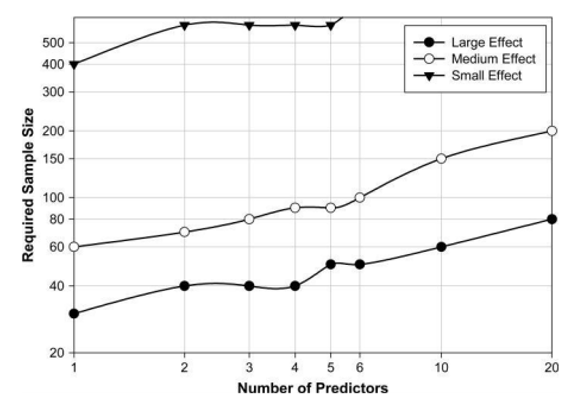
\includegraphics{Field_s223.png}

\hypertarget{de-uavhengige-variablene-er-additiv-for-den-avhengige-variabelen}{%
\paragraph{De uavhengige variablene er additiv for den avhengige variabelen}\label{de-uavhengige-variablene-er-additiv-for-den-avhengige-variabelen}}

Denne forutsetningen gjelder om man har minst to uavhengige variabler - altså i multippel regresjon. Med dette menes at vi må forvente at variasjonen i den avhengige variabelen er en funksjon av sum av endringer i de uavhengige variablene. Vi kan også uttrykke dette som at effekten av den uavhengige variabelen \(x_1\) på den avhengige variabelen \(y\) er uavhengig av eventuelle andre uavhengige variablers effekt på \(y\). Forutsetningen om additivitet betyr altså at det ikke er interaksjon mellom to eller flere uavhengige variabler.
Med andre ord, hvis effekten av \(x_1\) på \(y\) er avhengig av hvordan \(x_2...x_n\) påvirker \(y\) brytes forutsetningen om additivitet. I praksis er det imidlertid ikke uvanlig at denne forutsetningen brytes i en eller annen grad.

La oss vise dette med et eksempel fra \citet{thraneAppliedRegressionAnalysis2019} (se figur 6.1). Dersom vi har data for kvinners og menns inntekt relatert til antall års utdannelse vil vi kunne se i en regresjonsanalyse at antall års utdanning predikerer inntekt. Forutsetningen om additivitet sier da at antall års utdanning har lik effekt på inntekt for menn og kvinner. Slik er det imidlertid ikke. Generisk kan det framstilles som i grafen under:

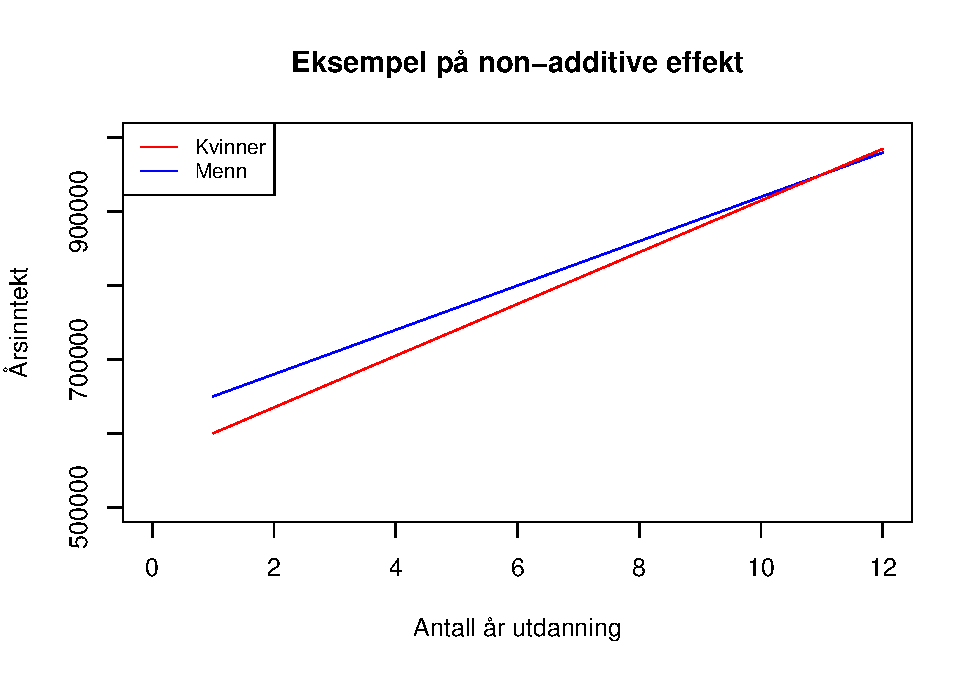
\includegraphics{02_Kap_2_files/figure-latex/unnamed-chunk-46-1.pdf}

Vi ser at linjene har ulikt stigningstall. Kvinner starter under menn, men har et høyere stigningstall. Det vil si at kvinner har større effekt av et (ekstra) års utdanning enn menn. Da er forutsetningen om additivitet brutt. Som \citet{thraneAppliedRegressionAnalysis2019} påpeker: ``Additivity thus means \emph{parallel} regression lines''.

Vi kan altså sjekke dette ved å kjøre to regresjonsanalyser. En annen måte, som vi ikke går inn på her, er å lage en interaksjonsvariabel som vi dernest bruker i modellen. En interaksjonsvariabel er et produkt av (minst) to uavhengige variabler.

La oss se på et annet eksempel for å vise interaksjonsvariabel og -effekt basert på et eksempel fra \citet{thomasAdditiveAssumptionMultiple2017}.

\begin{Shaded}
\begin{Highlighting}[]
\CommentTok{\# Bruker pakken: ISLR}
\FunctionTok{data}\NormalTok{(Carseats)}
\CommentTok{\# Bruker pakken: summarytools}
\NormalTok{summarytools}\SpecialCharTok{::}\FunctionTok{descr}\NormalTok{(Carseats, }\AttributeTok{stats =} \StringTok{"common"}\NormalTok{)}
\CommentTok{\#\textgreater{} Non{-}numerical variable(s) ignored: ShelveLoc, Urban, US}
\CommentTok{\#\textgreater{} Descriptive Statistics  }
\CommentTok{\#\textgreater{} Carseats  }
\CommentTok{\#\textgreater{} N: 400  }
\CommentTok{\#\textgreater{} }
\CommentTok{\#\textgreater{}                   Advertising      Age   CompPrice   Education   Income   Population    Price    Sales}
\CommentTok{\#\textgreater{} {-}{-}{-}{-}{-}{-}{-}{-}{-}{-}{-}{-}{-}{-}{-} {-}{-}{-}{-}{-}{-}{-}{-}{-}{-}{-}{-}{-} {-}{-}{-}{-}{-}{-}{-}{-} {-}{-}{-}{-}{-}{-}{-}{-}{-}{-}{-} {-}{-}{-}{-}{-}{-}{-}{-}{-}{-}{-} {-}{-}{-}{-}{-}{-}{-}{-} {-}{-}{-}{-}{-}{-}{-}{-}{-}{-}{-}{-} {-}{-}{-}{-}{-}{-}{-}{-} {-}{-}{-}{-}{-}{-}{-}{-}}
\CommentTok{\#\textgreater{}            Mean          6.64    53.32      124.97       13.90    68.66       264.84   115.80     7.50}
\CommentTok{\#\textgreater{}         Std.Dev          6.65    16.20       15.33        2.62    27.99       147.38    23.68     2.82}
\CommentTok{\#\textgreater{}             Min          0.00    25.00       77.00       10.00    21.00        10.00    24.00     0.00}
\CommentTok{\#\textgreater{}          Median          5.00    54.50      125.00       14.00    69.00       272.00   117.00     7.49}
\CommentTok{\#\textgreater{}             Max         29.00    80.00      175.00       18.00   120.00       509.00   191.00    16.27}
\CommentTok{\#\textgreater{}         N.Valid        400.00   400.00      400.00      400.00   400.00       400.00   400.00   400.00}
\CommentTok{\#\textgreater{}       Pct.Valid        100.00   100.00      100.00      100.00   100.00       100.00   100.00   100.00}
\end{Highlighting}
\end{Shaded}

Datasettet inneholder ti variabler i tillegg til det vi vil bruke som avhengig variabel: Sales. Vi vil altså se om vi kan bruke de ni variablene til å predikere salg.

\begin{Shaded}
\begin{Highlighting}[]
\CommentTok{\# Bruker pakken: olsrr}
\NormalTok{saleslm }\OtherTok{\textless{}{-}} \FunctionTok{ols\_regress}\NormalTok{(Sales}\SpecialCharTok{\textasciitilde{}}\NormalTok{. ,}\AttributeTok{data =}\NormalTok{ Carseats)}
\NormalTok{saleslm}
\CommentTok{\#\textgreater{}                         Model Summary                          }
\CommentTok{\#\textgreater{} {-}{-}{-}{-}{-}{-}{-}{-}{-}{-}{-}{-}{-}{-}{-}{-}{-}{-}{-}{-}{-}{-}{-}{-}{-}{-}{-}{-}{-}{-}{-}{-}{-}{-}{-}{-}{-}{-}{-}{-}{-}{-}{-}{-}{-}{-}{-}{-}{-}{-}{-}{-}{-}{-}{-}{-}{-}{-}{-}{-}{-}{-}}
\CommentTok{\#\textgreater{} R                       0.935       RMSE                1.019 }
\CommentTok{\#\textgreater{} R{-}Squared               0.873       Coef. Var          13.592 }
\CommentTok{\#\textgreater{} Adj. R{-}Squared          0.870       MSE                 1.038 }
\CommentTok{\#\textgreater{} Pred R{-}Squared          0.865       MAE                 0.804 }
\CommentTok{\#\textgreater{} {-}{-}{-}{-}{-}{-}{-}{-}{-}{-}{-}{-}{-}{-}{-}{-}{-}{-}{-}{-}{-}{-}{-}{-}{-}{-}{-}{-}{-}{-}{-}{-}{-}{-}{-}{-}{-}{-}{-}{-}{-}{-}{-}{-}{-}{-}{-}{-}{-}{-}{-}{-}{-}{-}{-}{-}{-}{-}{-}{-}{-}{-}}
\CommentTok{\#\textgreater{}  RMSE: Root Mean Square Error }
\CommentTok{\#\textgreater{}  MSE: Mean Square Error }
\CommentTok{\#\textgreater{}  MAE: Mean Absolute Error }
\CommentTok{\#\textgreater{} }
\CommentTok{\#\textgreater{}                                 ANOVA                                  }
\CommentTok{\#\textgreater{} {-}{-}{-}{-}{-}{-}{-}{-}{-}{-}{-}{-}{-}{-}{-}{-}{-}{-}{-}{-}{-}{-}{-}{-}{-}{-}{-}{-}{-}{-}{-}{-}{-}{-}{-}{-}{-}{-}{-}{-}{-}{-}{-}{-}{-}{-}{-}{-}{-}{-}{-}{-}{-}{-}{-}{-}{-}{-}{-}{-}{-}{-}{-}{-}{-}{-}{-}{-}{-}{-}}
\CommentTok{\#\textgreater{}                 Sum of                                                }
\CommentTok{\#\textgreater{}                Squares         DF    Mean Square       F         Sig. }
\CommentTok{\#\textgreater{} {-}{-}{-}{-}{-}{-}{-}{-}{-}{-}{-}{-}{-}{-}{-}{-}{-}{-}{-}{-}{-}{-}{-}{-}{-}{-}{-}{-}{-}{-}{-}{-}{-}{-}{-}{-}{-}{-}{-}{-}{-}{-}{-}{-}{-}{-}{-}{-}{-}{-}{-}{-}{-}{-}{-}{-}{-}{-}{-}{-}{-}{-}{-}{-}{-}{-}{-}{-}{-}{-}}
\CommentTok{\#\textgreater{} Regression    2779.441         11        252.676    243.372    0.0000 }
\CommentTok{\#\textgreater{} Residual       402.834        388          1.038                      }
\CommentTok{\#\textgreater{} Total         3182.275        399                                     }
\CommentTok{\#\textgreater{} {-}{-}{-}{-}{-}{-}{-}{-}{-}{-}{-}{-}{-}{-}{-}{-}{-}{-}{-}{-}{-}{-}{-}{-}{-}{-}{-}{-}{-}{-}{-}{-}{-}{-}{-}{-}{-}{-}{-}{-}{-}{-}{-}{-}{-}{-}{-}{-}{-}{-}{-}{-}{-}{-}{-}{-}{-}{-}{-}{-}{-}{-}{-}{-}{-}{-}{-}{-}{-}{-}}
\CommentTok{\#\textgreater{} }
\CommentTok{\#\textgreater{}                                      Parameter Estimates                                      }
\CommentTok{\#\textgreater{} {-}{-}{-}{-}{-}{-}{-}{-}{-}{-}{-}{-}{-}{-}{-}{-}{-}{-}{-}{-}{-}{-}{-}{-}{-}{-}{-}{-}{-}{-}{-}{-}{-}{-}{-}{-}{-}{-}{-}{-}{-}{-}{-}{-}{-}{-}{-}{-}{-}{-}{-}{-}{-}{-}{-}{-}{-}{-}{-}{-}{-}{-}{-}{-}{-}{-}{-}{-}{-}{-}{-}{-}{-}{-}{-}{-}{-}{-}{-}{-}{-}{-}{-}{-}{-}{-}{-}{-}{-}{-}{-}{-}{-}}
\CommentTok{\#\textgreater{}           model      Beta    Std. Error    Std. Beta       t        Sig      lower     upper }
\CommentTok{\#\textgreater{} {-}{-}{-}{-}{-}{-}{-}{-}{-}{-}{-}{-}{-}{-}{-}{-}{-}{-}{-}{-}{-}{-}{-}{-}{-}{-}{-}{-}{-}{-}{-}{-}{-}{-}{-}{-}{-}{-}{-}{-}{-}{-}{-}{-}{-}{-}{-}{-}{-}{-}{-}{-}{-}{-}{-}{-}{-}{-}{-}{-}{-}{-}{-}{-}{-}{-}{-}{-}{-}{-}{-}{-}{-}{-}{-}{-}{-}{-}{-}{-}{-}{-}{-}{-}{-}{-}{-}{-}{-}{-}{-}{-}{-}}
\CommentTok{\#\textgreater{}     (Intercept)     5.661         0.603                   9.380    0.000     4.474     6.847 }
\CommentTok{\#\textgreater{}       CompPrice     0.093         0.004        0.504     22.378    0.000     0.085     0.101 }
\CommentTok{\#\textgreater{}          Income     0.016         0.002        0.157      8.565    0.000     0.012     0.019 }
\CommentTok{\#\textgreater{}     Advertising     0.123         0.011        0.290     11.066    0.000     0.101     0.145 }
\CommentTok{\#\textgreater{}      Population     0.000         0.000        0.011      0.561    0.575    {-}0.001     0.001 }
\CommentTok{\#\textgreater{}           Price    {-}0.095         0.003       {-}0.799    {-}35.700    0.000    {-}0.101    {-}0.090 }
\CommentTok{\#\textgreater{}   ShelveLocGood     4.850         0.153        0.703     31.678    0.000     4.549     5.151 }
\CommentTok{\#\textgreater{} ShelveLocMedium     1.957         0.126        0.345     15.516    0.000     1.709     2.205 }
\CommentTok{\#\textgreater{}             Age    {-}0.046         0.003       {-}0.264    {-}14.472    0.000    {-}0.052    {-}0.040 }
\CommentTok{\#\textgreater{}       Education    {-}0.021         0.020       {-}0.020     {-}1.070    0.285    {-}0.060     0.018 }
\CommentTok{\#\textgreater{}        UrbanYes     0.123         0.113        0.020      1.088    0.277    {-}0.099     0.345 }
\CommentTok{\#\textgreater{}           USYes    {-}0.184         0.150       {-}0.031     {-}1.229    0.220    {-}0.479     0.111 }
\CommentTok{\#\textgreater{} {-}{-}{-}{-}{-}{-}{-}{-}{-}{-}{-}{-}{-}{-}{-}{-}{-}{-}{-}{-}{-}{-}{-}{-}{-}{-}{-}{-}{-}{-}{-}{-}{-}{-}{-}{-}{-}{-}{-}{-}{-}{-}{-}{-}{-}{-}{-}{-}{-}{-}{-}{-}{-}{-}{-}{-}{-}{-}{-}{-}{-}{-}{-}{-}{-}{-}{-}{-}{-}{-}{-}{-}{-}{-}{-}{-}{-}{-}{-}{-}{-}{-}{-}{-}{-}{-}{-}{-}{-}{-}{-}{-}{-}}
\end{Highlighting}
\end{Shaded}

Denne modellen kan altså forklare 87 \% av variansen i Sales.
Vi kan imidlertid mistenke at det kan være en interaksjon mellom variablene Income og Population - jo større befolkning, jo større inntekt tilgjengelig.

\begin{Shaded}
\begin{Highlighting}[]
\CommentTok{\# Base R}
\NormalTok{saleslm2 }\OtherTok{\textless{}{-}} \FunctionTok{lm}\NormalTok{(Sales}\SpecialCharTok{\textasciitilde{}}\NormalTok{. ,Carseats)}
\NormalTok{saleslm1 }\OtherTok{\textless{}{-}} \FunctionTok{lm}\NormalTok{(Sales}\SpecialCharTok{\textasciitilde{}}\NormalTok{.}\SpecialCharTok{+}\NormalTok{Population}\SpecialCharTok{*}\NormalTok{Income, Carseats)}
\CommentTok{\# Bruker pakken: car}
\FunctionTok{compareCoefs}\NormalTok{(saleslm2, saleslm1)}
\CommentTok{\#\textgreater{} Calls:}
\CommentTok{\#\textgreater{} 1: lm(formula = Sales \textasciitilde{} ., data = Carseats)}
\CommentTok{\#\textgreater{} 2: lm(formula = Sales \textasciitilde{} . + Population * Income, data = }
\CommentTok{\#\textgreater{}   Carseats)}
\CommentTok{\#\textgreater{} }
\CommentTok{\#\textgreater{}                     Model 1   Model 2}
\CommentTok{\#\textgreater{} (Intercept)           5.661     6.195}
\CommentTok{\#\textgreater{} SE                    0.603     0.644}
\CommentTok{\#\textgreater{}                                      }
\CommentTok{\#\textgreater{} CompPrice           0.09282   0.09262}
\CommentTok{\#\textgreater{} SE                  0.00415   0.00413}
\CommentTok{\#\textgreater{}                                      }
\CommentTok{\#\textgreater{} Income              0.01580   0.00797}
\CommentTok{\#\textgreater{} SE                  0.00185   0.00387}
\CommentTok{\#\textgreater{}                                      }
\CommentTok{\#\textgreater{} Advertising          0.1231    0.1237}
\CommentTok{\#\textgreater{} SE                   0.0111    0.0111}
\CommentTok{\#\textgreater{}                                      }
\CommentTok{\#\textgreater{} Population         0.000208 {-}0.001811}
\CommentTok{\#\textgreater{} SE                 0.000370  0.000952}
\CommentTok{\#\textgreater{}                                      }
\CommentTok{\#\textgreater{} Price              {-}0.09536  {-}0.09511}
\CommentTok{\#\textgreater{} SE                  0.00267   0.00266}
\CommentTok{\#\textgreater{}                                      }
\CommentTok{\#\textgreater{} ShelveLocGood         4.850     4.859}
\CommentTok{\#\textgreater{} SE                    0.153     0.152}
\CommentTok{\#\textgreater{}                                      }
\CommentTok{\#\textgreater{} ShelveLocMedium       1.957     1.964}
\CommentTok{\#\textgreater{} SE                    0.126     0.125}
\CommentTok{\#\textgreater{}                                      }
\CommentTok{\#\textgreater{} Age                {-}0.04605  {-}0.04566}
\CommentTok{\#\textgreater{} SE                  0.00318   0.00317}
\CommentTok{\#\textgreater{}                                      }
\CommentTok{\#\textgreater{} Education           {-}0.0211   {-}0.0216}
\CommentTok{\#\textgreater{} SE                   0.0197    0.0196}
\CommentTok{\#\textgreater{}                                      }
\CommentTok{\#\textgreater{} UrbanYes              0.123     0.133}
\CommentTok{\#\textgreater{} SE                    0.113     0.112}
\CommentTok{\#\textgreater{}                                      }
\CommentTok{\#\textgreater{} USYes                {-}0.184    {-}0.216}
\CommentTok{\#\textgreater{} SE                    0.150     0.150}
\CommentTok{\#\textgreater{}                                      }
\CommentTok{\#\textgreater{} Income:Population           0.0000288}
\CommentTok{\#\textgreater{} SE                          0.0000125}
\CommentTok{\#\textgreater{} }
\end{Highlighting}
\end{Shaded}

Forskjellen mellom modellene ligger altså i den nederste koeffisienten (Income:Population) som da er den kombinerte og samtidige effekten av de to variablene. Vi ser at effekten er veldig liten, men grafisk kan vi også se interaksjonseffekten:

\begin{Shaded}
\begin{Highlighting}[]
\CommentTok{\# Bruker pakken: ggplot2}
\FunctionTok{ggplot}\NormalTok{(}\AttributeTok{data=}\NormalTok{Carseats, }\FunctionTok{aes}\NormalTok{(}\AttributeTok{x=}\NormalTok{Income, }\AttributeTok{y=}\NormalTok{Sales, }\AttributeTok{group=}\DecValTok{1}\NormalTok{)) }\SpecialCharTok{+}\FunctionTok{geom\_smooth}\NormalTok{(}\AttributeTok{method=}\NormalTok{lm,}\AttributeTok{se=}\NormalTok{F)}\SpecialCharTok{+} 
    \FunctionTok{geom\_smooth}\NormalTok{(}\FunctionTok{aes}\NormalTok{(Population,Sales), }\AttributeTok{method=}\NormalTok{lm, }\AttributeTok{se=}\NormalTok{F,}\AttributeTok{color=}\StringTok{"black"}\NormalTok{)}\SpecialCharTok{+}\FunctionTok{xlab}\NormalTok{(}\StringTok{"Income and Population"}\NormalTok{)}\SpecialCharTok{+}\FunctionTok{labs}\NormalTok{(}
        \AttributeTok{title=}\StringTok{"Inntekt i blått {-} Befolkning i svart"}\NormalTok{)}
\CommentTok{\#\textgreater{} \textasciigrave{}geom\_smooth()\textasciigrave{} using formula \textquotesingle{}y \textasciitilde{} x\textquotesingle{}}
\CommentTok{\#\textgreater{} \textasciigrave{}geom\_smooth()\textasciigrave{} using formula \textquotesingle{}y \textasciitilde{} x\textquotesingle{}}
\end{Highlighting}
\end{Shaded}

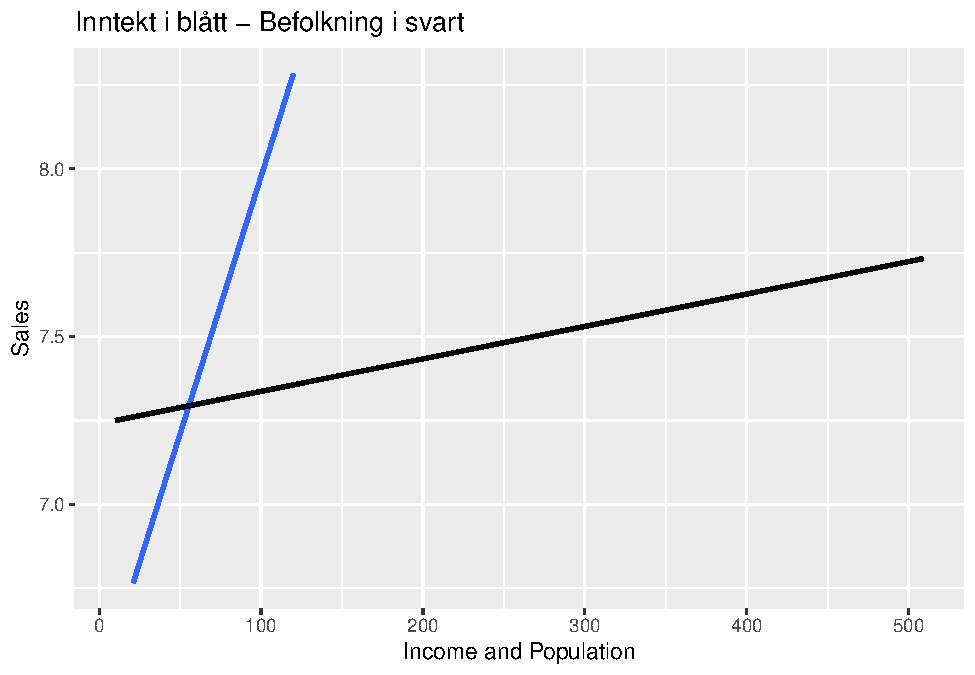
\includegraphics{02_Kap_2_files/figure-latex/unnamed-chunk-50-1.pdf}

Vi ser en klar interaksjon ved at linjene krysser (jfr. Thranes merknad om at forutsetningen om additivitet gir parallelle linjer).

I R har vi et hjelpemiddel i pakken \emph{interactions}:

\begin{Shaded}
\begin{Highlighting}[]
\CommentTok{\# Bruker pakken: interactions}
\FunctionTok{interact\_plot}\NormalTok{(saleslm1, }\AttributeTok{pred =}\NormalTok{ Population, }\AttributeTok{modx =}\NormalTok{ Income)}
\end{Highlighting}
\end{Shaded}

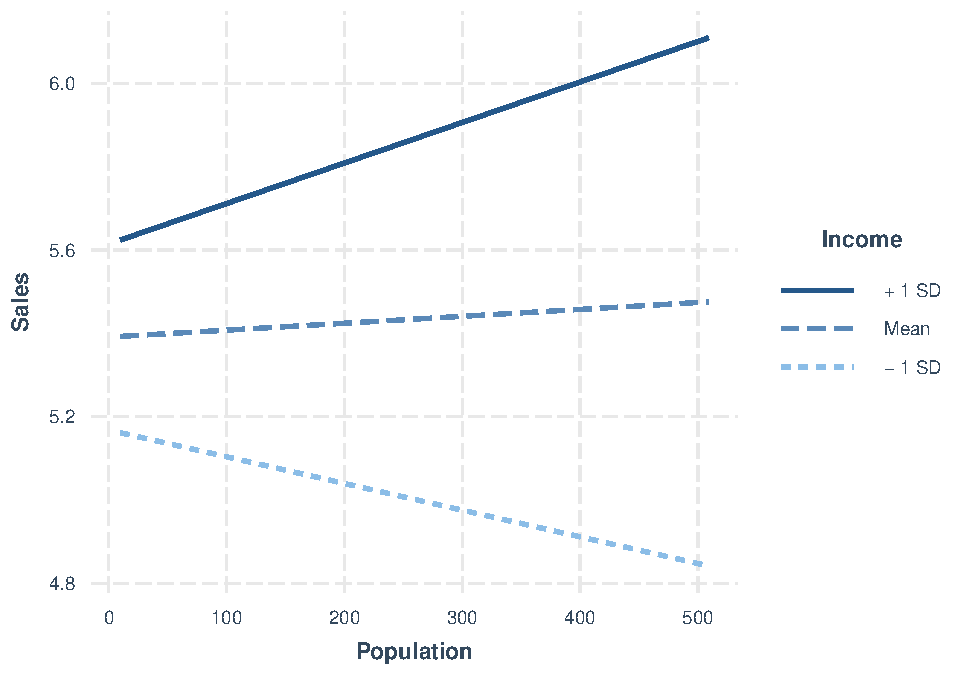
\includegraphics{02_Kap_2_files/figure-latex/unnamed-chunk-51-1.pdf}

Tolkningen av plottet fra pakken \emph{interactions} er den samme: Parallelle linjer indikerer fravær av interaksjoneseffekt, mens ikke-parallelle linjer indikerer tilstedeværelse av interaksjoneseffekt.

\begin{Shaded}
\begin{Highlighting}[]
\CommentTok{\# Bruker pakken: jtools}
\FunctionTok{summ}\NormalTok{(saleslm1)}
\end{Highlighting}
\end{Shaded}

\begin{table}[!h]
\centering
\begin{tabular}{lr}
\toprule
\cellcolor{gray!6}{Observations} & \cellcolor{gray!6}{400}\\
Dependent variable & Sales\\
\cellcolor{gray!6}{Type} & \cellcolor{gray!6}{OLS linear regression}\\
\bottomrule
\end{tabular}
\end{table} \begin{table}[!h]
\centering
\begin{tabular}{lr}
\toprule
\cellcolor{gray!6}{F(12,387)} & \cellcolor{gray!6}{225.99}\\
R² & 0.88\\
\cellcolor{gray!6}{Adj. R²} & \cellcolor{gray!6}{0.87}\\
\bottomrule
\end{tabular}
\end{table} \begin{table}[!h]
\centering
\begin{threeparttable}
\begin{tabular}{lrrrr}
\toprule
  & Est. & S.E. & t val. & p\\
\midrule
\cellcolor{gray!6}{(Intercept)} & \cellcolor{gray!6}{6.20} & \cellcolor{gray!6}{0.64} & \cellcolor{gray!6}{9.63} & \cellcolor{gray!6}{0.00}\\
CompPrice & 0.09 & 0.00 & 22.45 & 0.00\\
\cellcolor{gray!6}{Income} & \cellcolor{gray!6}{0.01} & \cellcolor{gray!6}{0.00} & \cellcolor{gray!6}{2.06} & \cellcolor{gray!6}{0.04}\\
Advertising & 0.12 & 0.01 & 11.18 & 0.00\\
\cellcolor{gray!6}{Population} & \cellcolor{gray!6}{-0.00} & \cellcolor{gray!6}{0.00} & \cellcolor{gray!6}{-1.90} & \cellcolor{gray!6}{0.06}\\
\addlinespace
Price & -0.10 & 0.00 & -35.77 & 0.00\\
\cellcolor{gray!6}{ShelveLocGood} & \cellcolor{gray!6}{4.86} & \cellcolor{gray!6}{0.15} & \cellcolor{gray!6}{31.90} & \cellcolor{gray!6}{0.00}\\
ShelveLocMedium & 1.96 & 0.13 & 15.65 & 0.00\\
\cellcolor{gray!6}{Age} & \cellcolor{gray!6}{-0.05} & \cellcolor{gray!6}{0.00} & \cellcolor{gray!6}{-14.41} & \cellcolor{gray!6}{0.00}\\
Education & -0.02 & 0.02 & -1.10 & 0.27\\
\addlinespace
\cellcolor{gray!6}{UrbanYes} & \cellcolor{gray!6}{0.13} & \cellcolor{gray!6}{0.11} & \cellcolor{gray!6}{1.18} & \cellcolor{gray!6}{0.24}\\
USYes & -0.22 & 0.15 & -1.44 & 0.15\\
\cellcolor{gray!6}{Income:Population} & \cellcolor{gray!6}{0.00} & \cellcolor{gray!6}{0.00} & \cellcolor{gray!6}{2.30} & \cellcolor{gray!6}{0.02}\\
\bottomrule
\end{tabular}
\begin{tablenotes}
\item Standard errors: OLS
\end{tablenotes}
\end{threeparttable}
\end{table}

Vi ser i tillegg at interaksjonseffekten (Income:Population) er statistisk signifikant.

\hypertarget{linearitet}{%
\paragraph{Linearitet}\label{linearitet}}

Vi tar, som navnet ``linær regresjonsanalyse'' ganske klart indikerer, utgangspunkt i at forholdet mellom den/de uavhengige varaibelen(e) og den avhengige variabelen kan beskrives som en lineær funksjon (se for eksempel \citet{ringdalEnhetOgMangfold2007}). Sammenhengen mellom variablene må ikke være perfekt lineær, men må i hvert fall være tilnærmet lineær.

Vi har allerede sett en grafisk framstilling under punktet analyse av dataene som lar oss visuelt vurdere denne forutsetningen:

\begin{Shaded}
\begin{Highlighting}[]
\CommentTok{\# Bruker pakken: car}
\FunctionTok{scatterplot}\NormalTok{(Adverts }\SpecialCharTok{\textasciitilde{}}\NormalTok{ Sales, }\AttributeTok{data =}\NormalTok{ Field\_OLS\_data)}
\end{Highlighting}
\end{Shaded}

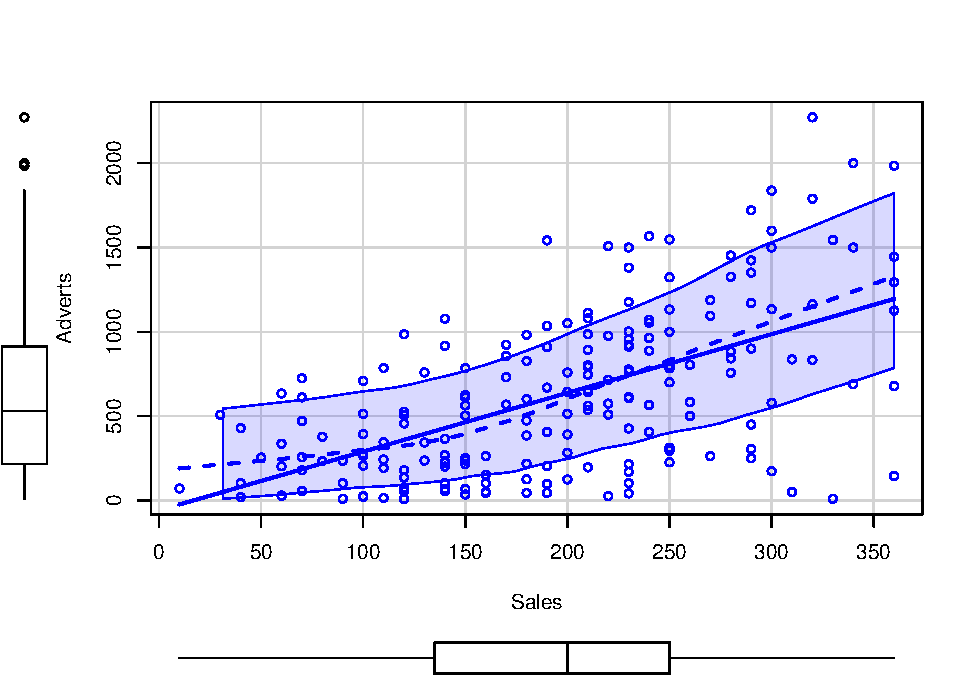
\includegraphics{02_Kap_2_files/figure-latex/unnamed-chunk-53-1.pdf}

Den stiplede linjen som buer ca midt i det skraverte området gjør ingen forutsetninger, men plotter bare dataene (ofte kalt ``scatterplot smoother''). Vi kan vurdere om denne er nærme eller langt fra en rett linje. I grafen over ligger det både en stiplet buet linje og en rett linje (regresjonslinje). I vårt tilfelle vil vi raskt konkludere med at forholdet mellom de to variablene er tilnærmet lineært.

\hypertarget{residualene-skal-vuxe6re-normalfordelte}{%
\paragraph{Residualene skal være normalfordelte}\label{residualene-skal-vuxe6re-normalfordelte}}

Forutsetningen er at residualene i modellen er tilfeldige, normalfordelte variabler med gjennomsnittsverdi 0 \citep{fieldDiscoveringStatisticsUsing2012}, hvilket innebærer at forskjellen mellom modellen og de observerte dataene er 0 eller nær 0 i de fleste tilfeller (og at ulikhet skyldes tilfeldigheter). Poenget her er at dersom regresjonsmodellen er god skal det være omtrent like stor sannsynlighet for at den underestimerer som at den overestimerer. Er den det vil fordelingen være tilnærmet symmetrisk (perfekt normalfordeling vil i praksis ikke inntreffe).

En tilnærming til å se på denne forutsetningen er å se på et histogram over residualene. Når vi lagrer regresjonsmodellen som et objekt (i R) kan vi se hvilke parametere som lagres i modellen:

\begin{Shaded}
\begin{Highlighting}[]
\CommentTok{\# Base R}
\FunctionTok{names}\NormalTok{(FieldOLS\_reg)}
\CommentTok{\#\textgreater{}  [1] "coefficients"  "residuals"     "effects"      }
\CommentTok{\#\textgreater{}  [4] "rank"          "fitted.values" "assign"       }
\CommentTok{\#\textgreater{}  [7] "qr"            "df.residual"   "xlevels"      }
\CommentTok{\#\textgreater{} [10] "call"          "terms"         "model"}
\end{Highlighting}
\end{Shaded}

Residualene lagres altså i modellen og vi kan plotte ut disse:

\begin{Shaded}
\begin{Highlighting}[]
\CommentTok{\# Base R}

\NormalTok{FieldOLS\_reg }\OtherTok{\textless{}{-}} \FunctionTok{lm}\NormalTok{(Sales }\SpecialCharTok{\textasciitilde{}}\NormalTok{ Adverts, Field\_OLS\_data)}

\FunctionTok{hist}\NormalTok{(FieldOLS\_reg}\SpecialCharTok{$}\NormalTok{residuals)}
\end{Highlighting}
\end{Shaded}

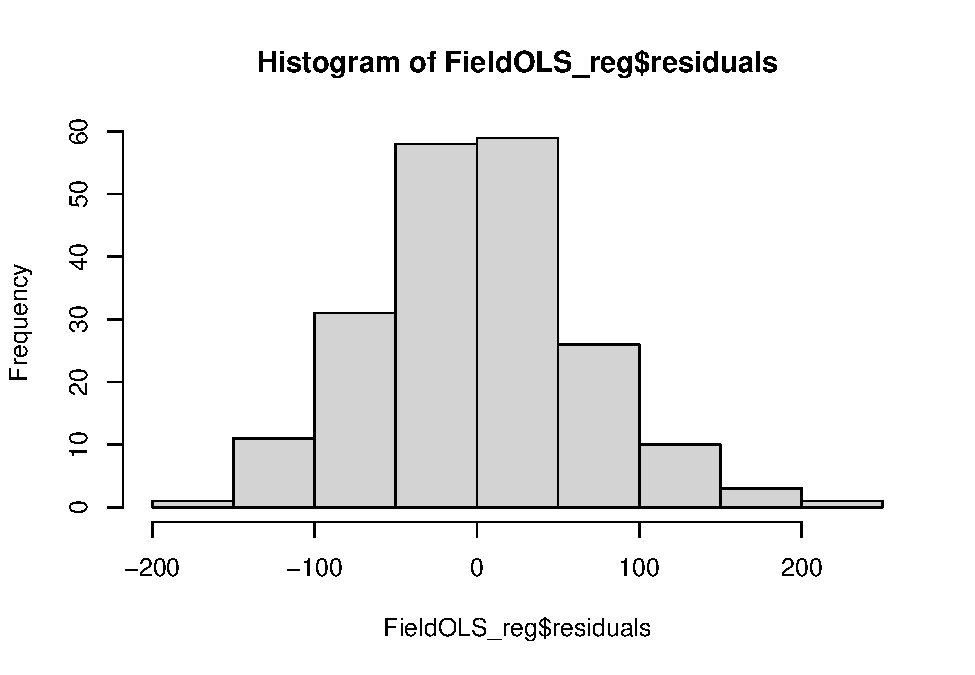
\includegraphics{02_Kap_2_files/figure-latex/unnamed-chunk-55-1.pdf}

\begin{Shaded}
\begin{Highlighting}[]

\NormalTok{FieldOLSresid }\OtherTok{\textless{}{-}}\NormalTok{ FieldOLS\_reg}\SpecialCharTok{$}\NormalTok{residuals}

\NormalTok{plott3 }\OtherTok{\textless{}{-}} \FunctionTok{ggplot}\NormalTok{(}\AttributeTok{data =}\NormalTok{ FieldOLS\_reg, }\FunctionTok{aes}\NormalTok{(FieldOLS\_reg}\SpecialCharTok{$}\NormalTok{residuals)) }\SpecialCharTok{+} 
  \FunctionTok{geom\_histogram}\NormalTok{(}\AttributeTok{bins =} \DecValTok{10}\NormalTok{, }\AttributeTok{color =} \StringTok{"\#000000"}\NormalTok{, }\AttributeTok{fill =} \StringTok{"\#0099F8"}\NormalTok{) }\SpecialCharTok{+}
    \FunctionTok{theme\_classic}\NormalTok{() }\SpecialCharTok{+}
    \FunctionTok{labs}\NormalTok{(}\AttributeTok{title =} \StringTok{\textquotesingle{}Histogram av residualer\textquotesingle{}}\NormalTok{, }\AttributeTok{x =} \StringTok{\textquotesingle{}Residualer\textquotesingle{}}\NormalTok{, }\AttributeTok{y =} \StringTok{\textquotesingle{}Antall\textquotesingle{}}\NormalTok{)}

\NormalTok{plott3}
\end{Highlighting}
\end{Shaded}

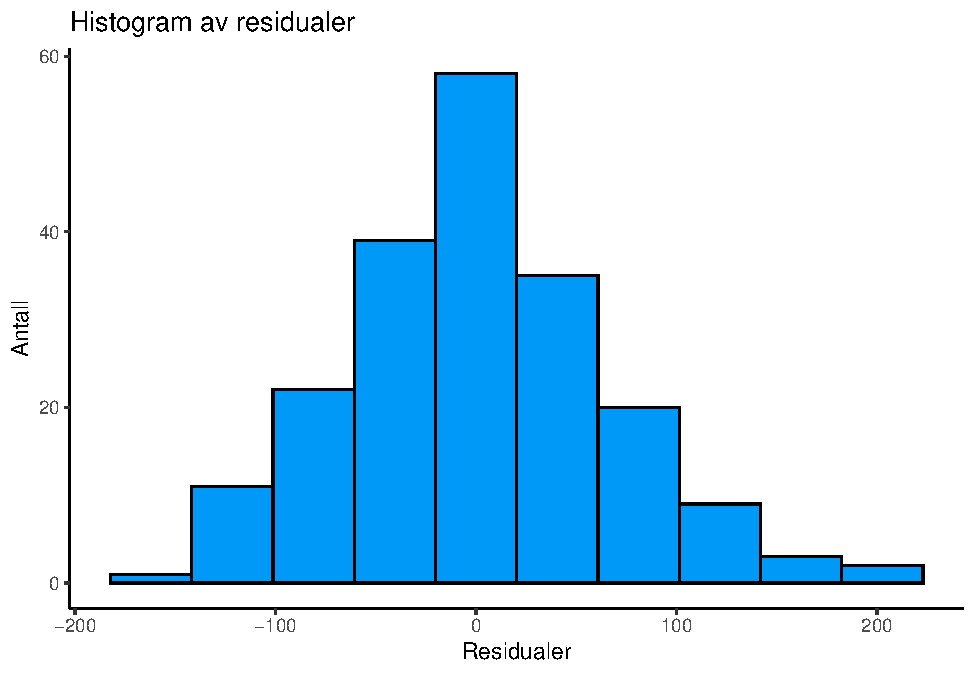
\includegraphics{02_Kap_2_files/figure-latex/unnamed-chunk-55-2.pdf}

Vi kan også se på et Q-Q plott og hente ut testverdier for ulike normalitetstester:

\begin{Shaded}
\begin{Highlighting}[]
\CommentTok{\# Bruker pakken: olsrr}
\FunctionTok{ols\_plot\_resid\_qq}\NormalTok{(FieldOLS\_reg)}
\end{Highlighting}
\end{Shaded}

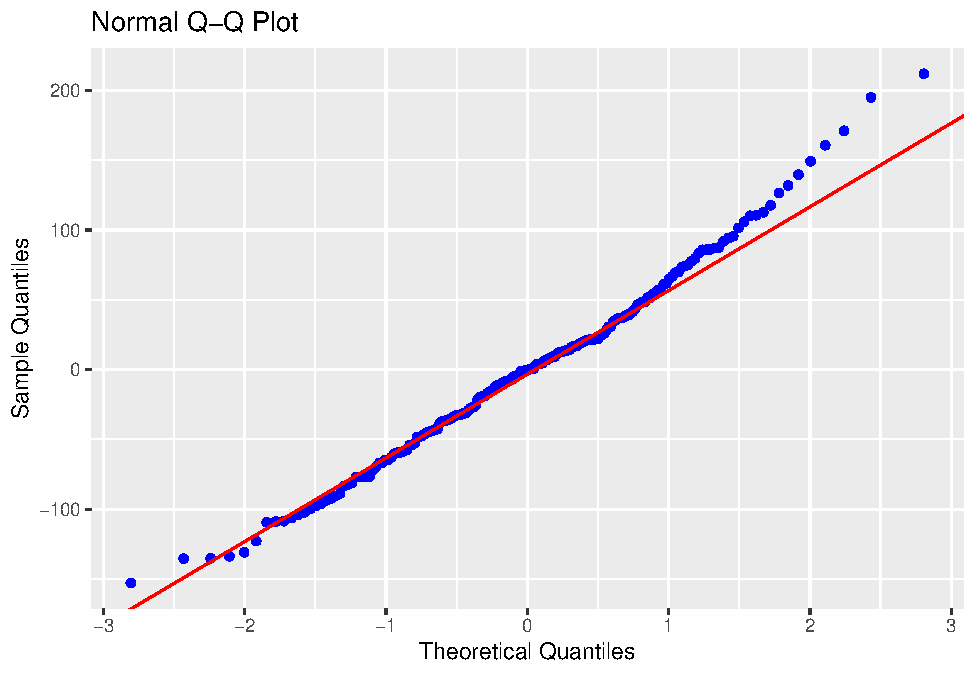
\includegraphics{02_Kap_2_files/figure-latex/unnamed-chunk-56-1.pdf}

\begin{Shaded}
\begin{Highlighting}[]
\FunctionTok{ols\_test\_normality}\NormalTok{(FieldOLS\_reg)}
\CommentTok{\#\textgreater{} {-}{-}{-}{-}{-}{-}{-}{-}{-}{-}{-}{-}{-}{-}{-}{-}{-}{-}{-}{-}{-}{-}{-}{-}{-}{-}{-}{-}{-}{-}{-}{-}{-}{-}{-}{-}{-}{-}{-}{-}{-}{-}{-}{-}{-}{-}{-}}
\CommentTok{\#\textgreater{}        Test             Statistic       pvalue  }
\CommentTok{\#\textgreater{} {-}{-}{-}{-}{-}{-}{-}{-}{-}{-}{-}{-}{-}{-}{-}{-}{-}{-}{-}{-}{-}{-}{-}{-}{-}{-}{-}{-}{-}{-}{-}{-}{-}{-}{-}{-}{-}{-}{-}{-}{-}{-}{-}{-}{-}{-}{-}}
\CommentTok{\#\textgreater{} Shapiro{-}Wilk              0.9899         0.1757 }
\CommentTok{\#\textgreater{} Kolmogorov{-}Smirnov        0.0634         0.3970 }
\CommentTok{\#\textgreater{} Cramer{-}von Mises          16.055         0.0000 }
\CommentTok{\#\textgreater{} Anderson{-}Darling          0.4298         0.3057 }
\CommentTok{\#\textgreater{} {-}{-}{-}{-}{-}{-}{-}{-}{-}{-}{-}{-}{-}{-}{-}{-}{-}{-}{-}{-}{-}{-}{-}{-}{-}{-}{-}{-}{-}{-}{-}{-}{-}{-}{-}{-}{-}{-}{-}{-}{-}{-}{-}{-}{-}{-}{-}}
\end{Highlighting}
\end{Shaded}

Q-Q plottet viser noe avvik.

En hendig graf er også et plott av residualene på y-aksen og ``fitted values'' på x-aksen:

\begin{Shaded}
\begin{Highlighting}[]
\CommentTok{\# Bruker pakken: olsrr}
\FunctionTok{ols\_plot\_resid\_fit}\NormalTok{(FieldOLS\_reg)}
\end{Highlighting}
\end{Shaded}

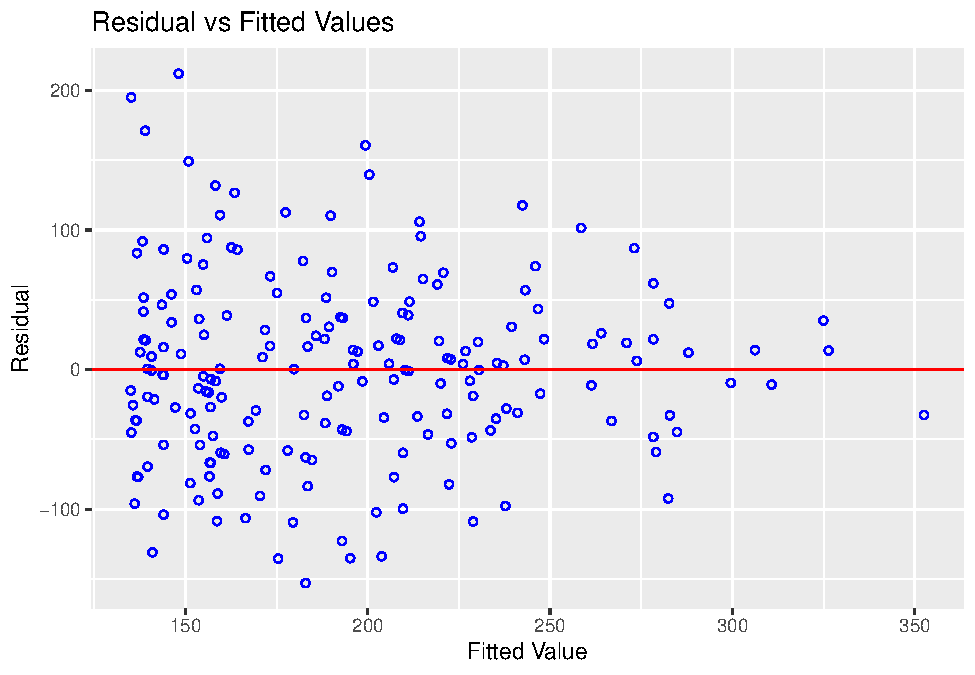
\includegraphics{02_Kap_2_files/figure-latex/unnamed-chunk-57-1.pdf}

I forhold til forutsetningen om normalfordelte residualer skal være spredd tilfeldig rundt 0.

Sett under ett kan det i dette tilfellet se ut som at residualene er tilnærmet (nok) normalfordeling.

\hypertarget{fravuxe6r-av-multikolinearitet}{%
\paragraph{Fravær av multikolinearitet}\label{fravuxe6r-av-multikolinearitet}}

Multikolinearitet innebærer at det er korrelasjon mellom de uavhengige varaiblene (i multippel regresjon). Det kan ofte forekomme at vi har en viss korrelasjon, men hvis korrelasjonen blir stor blir det vanskelig å skille mellom effekten den enkelte uavhengige variabel har på den avhengige variabelen.

Multikolinearitet inntreffer dersom vi har sterk korrelasjon mellom to eller flere av de uavhengige variablene. Multikollinearitet handler altså om det innbyrdes forholdet mellom de uavhengige variablene. Hvis disse er for høyt korrelerte har vi multikollinearitet, altså at det kan være (tilnærmet) perfekt linearitet mellom to uavhengige variabler \citep{berryUnderstandingRegressionAssumptions1993} hvilket innebærer muligheten for at ingen av korrelasjonskoeffisientene er signifikante pga størrelsen på standardfeil. En perfekt kolinearitet har koeffisienten 1.

\citet{berryUnderstandingRegressionAssumptions1993} angir at angir at \(r=.9\) gir en dobling av standardfeil i regresjonskoeffisienten, og at selv \(0.5\) og \(0.6\) kan gi utfordringer for tolkningen av regresjonskoeffisientene. \citet{fieldDiscoveringStatisticsUsing2009} anser \(0.8\) til \(0.9\) som høy korrelasjon.

Samtidig sier \citet{pallantSPSSSurvivalManual2010} at det (naturligvis) bør være en viss korrelasjon mellom de uavhengige og den avhengige variabelen, og hevder de bør være på over \(0.3\), men samtidig at bivariat korrelasjon mellom de uavhengige variablene ikke bør være over \(0.7\).

Vi kan derfor sjekke for multikolinearitet gjennom å se på en korrelasjonsmatrisen:

\begin{Shaded}
\begin{Highlighting}[]
\CommentTok{\# Base R}
\NormalTok{FieldKorr }\OtherTok{\textless{}{-}} \FunctionTok{cor}\NormalTok{(Field\_OLS\_data, }\AttributeTok{method =} \StringTok{"pearson"}\NormalTok{)}
\FunctionTok{round}\NormalTok{(FieldKorr, }\DecValTok{2}\NormalTok{)}
\CommentTok{\#\textgreater{}         Adverts Sales Airplay Image}
\CommentTok{\#\textgreater{} Adverts    1.00  0.58    0.10  0.08}
\CommentTok{\#\textgreater{} Sales      0.58  1.00    0.60  0.33}
\CommentTok{\#\textgreater{} Airplay    0.10  0.60    1.00  0.18}
\CommentTok{\#\textgreater{} Image      0.08  0.33    0.18  1.00}
\end{Highlighting}
\end{Shaded}

Hvis vi følger \citet{pallantSPSSSurvivalManual2010} ser vi først at alle de tre uavhengige variablene korrelerer mellom \(0.33\) og \(0.60\) med den avhengige. De bivariate korrelasjonene mellom de uavhengige variablene erpå hhv. \(0.08\), \(0.10\) og \(0.18\). Ut fra korrelasjonsmatrisen bør det ikke være grunn til å frykte multikolinearitet.

Dette er aktuelt i multippel regresjonsanalyse, så for å vise dette lager vi en slik for datasettet til Field der vi inkluderer tre uavhengige variabler:

\begin{Shaded}
\begin{Highlighting}[]
\CommentTok{\# Base R}
\NormalTok{FieldOLS\_mult\_reg }\OtherTok{\textless{}{-}} \FunctionTok{lm}\NormalTok{(Sales }\SpecialCharTok{\textasciitilde{}}\NormalTok{ ., }\AttributeTok{data =}\NormalTok{ Field\_OLS\_data)}
\FunctionTok{brief}\NormalTok{(FieldOLS\_mult\_reg)}
\CommentTok{\#\textgreater{}            (Intercept) Adverts Airplay Image}
\CommentTok{\#\textgreater{} Estimate         {-}26.6 0.08488   3.367 11.09}
\CommentTok{\#\textgreater{} Std. Error        17.4 0.00692   0.278  2.44}
\CommentTok{\#\textgreater{} }
\CommentTok{\#\textgreater{}  Residual SD = 47.1 on 196 df, R{-}squared = 0.665}
\end{Highlighting}
\end{Shaded}

Vi kan også se på Variance Inflation Factor (VIF), som måler hvor mye variansen til en estimert regresjonskoeffisient øker pga. multikollinearitet.

\begin{Shaded}
\begin{Highlighting}[]
\CommentTok{\# Bruker pakken: olsrr}
\FunctionTok{ols\_vif\_tol}\NormalTok{(FieldOLS\_mult\_reg)}
\CommentTok{\#\textgreater{}   Variables Tolerance      VIF}
\CommentTok{\#\textgreater{} 1   Adverts 0.9856172 1.014593}
\CommentTok{\#\textgreater{} 2   Airplay 0.9592287 1.042504}
\CommentTok{\#\textgreater{} 3     Image 0.9629695 1.038455}
\end{Highlighting}
\end{Shaded}

\citet{myersClassicalModernRegression1990} og \citet{hairjr.MultivariateDataAnalysis2010} opererer med en akseptabel grense for VIF på 10.0 (toleranse på .1). Her er rådene (også) litt ulike. En VIF-verdi på 10 for VIF anses f.eks. i pakken ``olsrr'' i R (som vi har brukt over) som et tegn på alvorlig multikolinearitet \citep[jfr.][]{belsleyRegressionDiagnosticsIdentifying1980}. Der settes VIF på 4 som en grense der man bør se nærmere på om multikolinearitet kan være et problem. \citet{bowermanLinearStatisticalModels1990} tilføyer at snittet av VIF for de uavhengige variablene ikke bør være vesentlig over 1.

\hypertarget{fravuxe6r-av-heteroskedasisitet}{%
\paragraph{Fravær av heteroskedasisitet}\label{fravuxe6r-av-heteroskedasisitet}}

Variansen til residualene for de uavhengige variablene skal være lik \citep{milesApplyingRegressionCorrelation2001}. Heteroskedasitsitet innebærer at residualene ikke har konstant varianse (motsatt: vi ønsker lik varians i residualene over alle x-verdier og kaller dette homoskedastisitet). Hvis vi har homoskedastisitet predikerer modellen vår likt på alle predikerte verdier av Y, noe vi ønsker.

Variansen til residualen kan altså ikke avhenge av de uavhengige variablene, men være lik på alle nivåer av verdier for prediktorene. Dersom vi har heteroskedastisitet vil spredningen rundt regresjonslinja variere med X.

Forutsetningen om homoskedastisitet er godt illustrert av \citet{milesApplyingRegressionCorrelation2001}, s.100-101, fig.~4.22, 4.23 og 4.24:

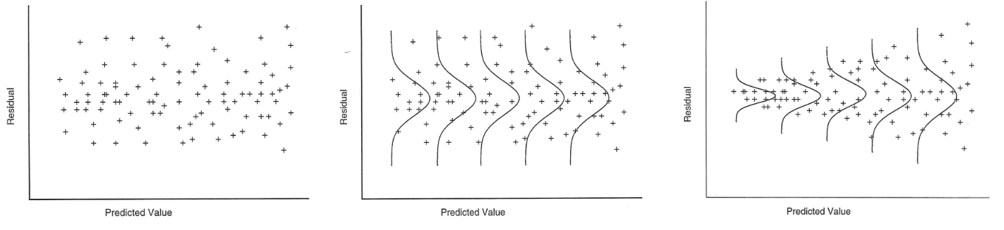
\includegraphics{Heteroskedasicity.png}

Figuren til venstre viser et scatterplot for residualer. I midten har vi samme fordeling av residualer med et antall normalfordelingskurver. Til høyre ser vi et alternativt scatterplot for residualer som bryter med forutsetningen om homoskedastisitet.

\citet{lovasStatistikkUniversiteterOg2013} illustrerer det samme slik i eksempelet om motorstørrelse og drivstofforbruk:

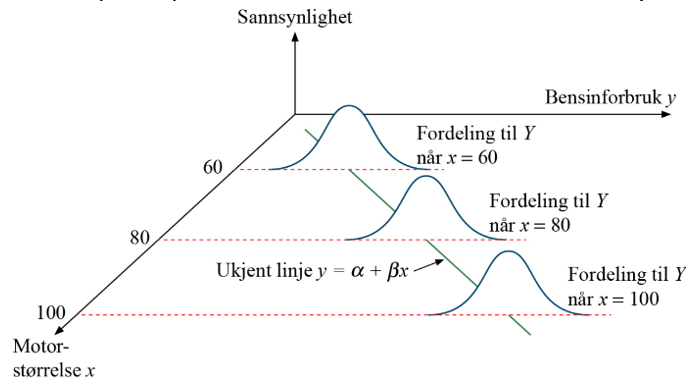
\includegraphics{Homoskedastisitet.png}

Variasjonen i residualene er like stor uansett verdien av x.

Den såkalte White's test vil også kunne være et godt hjelpemiddel:

\begin{Shaded}
\begin{Highlighting}[]
\CommentTok{\# Base R}
\NormalTok{FieldOLS\_mult2 }\OtherTok{\textless{}{-}} \FunctionTok{lm}\NormalTok{(Sales }\SpecialCharTok{\textasciitilde{}}\NormalTok{ Adverts }\SpecialCharTok{+}\NormalTok{ Airplay }\SpecialCharTok{+}\NormalTok{ Image, }\AttributeTok{data =}\NormalTok{ Field\_OLS\_data)}
\CommentTok{\# Bruker pakken: lmtest}
\FunctionTok{bptest}\NormalTok{(FieldOLS\_mult2, }\SpecialCharTok{\textasciitilde{}}\NormalTok{ Adverts}\SpecialCharTok{*}\NormalTok{Airplay}\SpecialCharTok{*}\NormalTok{Image }\SpecialCharTok{+} \FunctionTok{I}\NormalTok{(Adverts}\SpecialCharTok{\^{}}\DecValTok{2}\NormalTok{) }\SpecialCharTok{+} \FunctionTok{I}\NormalTok{(Airplay}\SpecialCharTok{\^{}}\DecValTok{2}\NormalTok{)}\SpecialCharTok{+} \FunctionTok{I}\NormalTok{(Image}\SpecialCharTok{\^{}}\DecValTok{2}\NormalTok{), }\AttributeTok{data =}\NormalTok{ Field\_OLS\_data)}
\CommentTok{\#\textgreater{} }
\CommentTok{\#\textgreater{}  studentized Breusch{-}Pagan test}
\CommentTok{\#\textgreater{} }
\CommentTok{\#\textgreater{} data:  FieldOLS\_mult2}
\CommentTok{\#\textgreater{} BP = 10.44, df = 10, p{-}value = 0.4027}
\end{Highlighting}
\end{Shaded}

Her ser vi at p-verdien er \(0.4027\), dvs. vi kan ikke forkaste nullhypotesen = vi har ikke grunn til å konkludere med at vi har heteroskedasisitet i regresjonsmodellen.

\hypertarget{fravuxe6r-av-autokorrelasjon}{%
\paragraph{Fravær av autokorrelasjon}\label{fravuxe6r-av-autokorrelasjon}}

Dette er typisk et problem i tidsserieanalyser eller geografiske analyser \citep[a.124]{eikemoKvantitativAnalyseMed2007}, der ``verdien på variabel X for enhet N i stor grad er bestemt av verdien på variabel X for enhet N-1''. Et annet kjent eksempel er fra aksjemarkedet: Hvis en aksje stiger i dag er det mer sannsynlig at den stiger i morgen. Verdien av aksjen i morgen avhenger (delvis) av verdien i dag. Verdiene i dataene autokorrelerer. Grad av autokorrelasjon er således et mål på forholdet mellom en variabels verdi på tidspunkt X og verdien på tidspunkt før X.

To tilfeldige observasjoner bør ikke ha korrelasjon i residualen. Dette kan testes gjennom en Durbin-Watson test \citep{durbinTestingSerialCorrelation1951}.
Durbin-Watson testen er en test på autokorrelasjon i residualene, og vil ha en verdi på mellom 0 og 4. Verdien 2 indikerer ingen autokorrelasjon. Verdier mellom 0 og 2 indikerer en positiv autokorrelasjon, mens verdier mellom 2 og 4 indikerer en negativ autokorrelasjon. En konservativ tommelfingerregel sier at verdier under 1 og over 3 er bekymringsfullt \citep{fieldDiscoveringStatisticsUsing2012}.

\begin{Shaded}
\begin{Highlighting}[]
\CommentTok{\# Bruker pakken: car}
\FunctionTok{durbinWatsonTest}\NormalTok{(FieldOLS\_reg)}
\CommentTok{\#\textgreater{}  lag Autocorrelation D{-}W Statistic p{-}value}
\CommentTok{\#\textgreater{}    1     {-}0.04394305      2.032324   0.762}
\CommentTok{\#\textgreater{}  Alternative hypothesis: rho != 0}
\end{Highlighting}
\end{Shaded}

Her viser verdien \(2.03\) noe som ikke gir grunn til bekymring.

\hypertarget{fravuxe6r-av-innflytelsesrike-observasjonercaser}{%
\paragraph{Fravær av innflytelsesrike observasjoner/caser}\label{fravuxe6r-av-innflytelsesrike-observasjonercaser}}

Vi så under punktet ``Analyse av dataene'' (se for eksempel Boxplottet av Adverts) at vi har noen observasjoner i modellen som kan defineres som uteliggere. Vi kan identifisere disse gjennom residualene:

\begin{Shaded}
\begin{Highlighting}[]
\CommentTok{\# Bruker pakken: olsrr}
\NormalTok{car}\SpecialCharTok{::}\FunctionTok{qqPlot}\NormalTok{(FieldOLS\_reg, }\AttributeTok{id.method=}\StringTok{"identify"}\NormalTok{, }\AttributeTok{main=}\StringTok{"Q{-}Q Plott"}\NormalTok{)}
\end{Highlighting}
\end{Shaded}

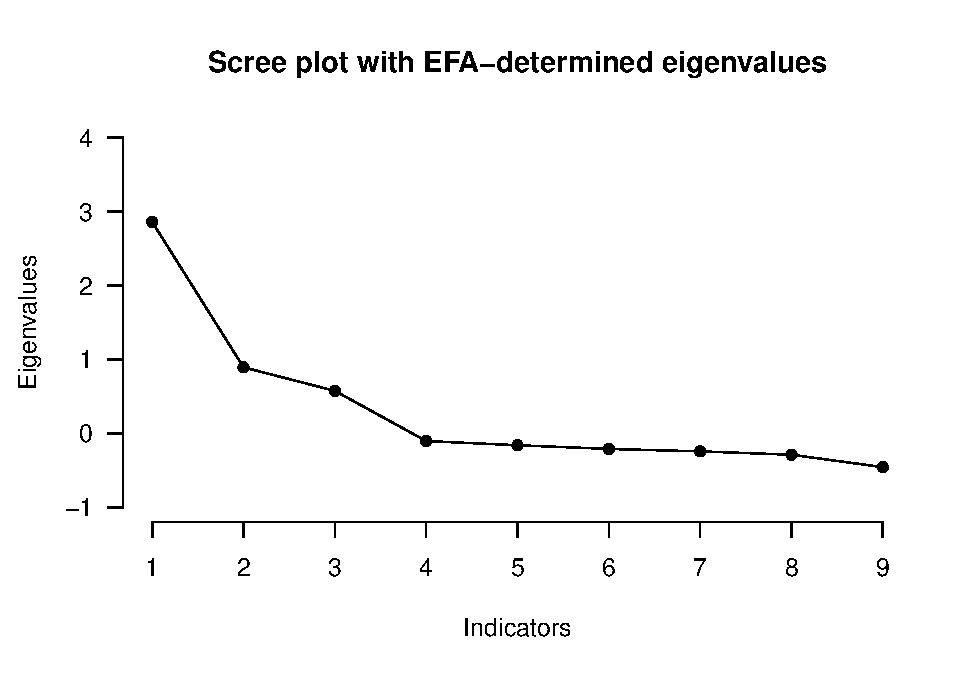
\includegraphics{02_Kap_2_files/figure-latex/unnamed-chunk-63-1.pdf}

\begin{verbatim}
#> [1]   1 169
\end{verbatim}

Vi ser at residualene for 1 og 169 identifiseres som statistisk signifikante uteliggere

\hypertarget{hampel-filter}{%
\subparagraph{Hampel filter}\label{hampel-filter}}

Hampel filter innebærer at man ser alle observasjoner som ligger utenfor intervallet \(median +/- 3 median\ absolute\ deviation\ (MAS)\).

\begin{Shaded}
\begin{Highlighting}[]
\CommentTok{\#Base R}
\NormalTok{nedregrense }\OtherTok{\textless{}{-}} \FunctionTok{median}\NormalTok{(Field\_OLS\_data}\SpecialCharTok{$}\NormalTok{Adverts) }\SpecialCharTok{{-}} \DecValTok{3}\SpecialCharTok{*}\NormalTok{(}\FunctionTok{mad}\NormalTok{(Field\_OLS\_data}\SpecialCharTok{$}\NormalTok{Adverts, }\AttributeTok{constant =} \DecValTok{1}\NormalTok{))}
\NormalTok{nedregrense}
\CommentTok{\#\textgreater{} [1] {-}457.7405}

\NormalTok{ovregrense }\OtherTok{\textless{}{-}} \FunctionTok{median}\NormalTok{(Field\_OLS\_data}\SpecialCharTok{$}\NormalTok{Adverts) }\SpecialCharTok{+} \DecValTok{3}\SpecialCharTok{*}\NormalTok{(}\FunctionTok{mad}\NormalTok{(Field\_OLS\_data}\SpecialCharTok{$}\NormalTok{Adverts, }\AttributeTok{constant =} \DecValTok{1}\NormalTok{))}
\NormalTok{ovregrense}
\CommentTok{\#\textgreater{} [1] 1521.572}

\NormalTok{uteligger\_ind }\OtherTok{\textless{}{-}} \FunctionTok{which}\NormalTok{(Field\_OLS\_data}\SpecialCharTok{$}\NormalTok{Adverts }\SpecialCharTok{\textless{}}\NormalTok{ nedregrense }\SpecialCharTok{|}\NormalTok{Field\_OLS\_data}\SpecialCharTok{$}\NormalTok{Adverts }\SpecialCharTok{\textgreater{}}\NormalTok{ ovregrense)}
\NormalTok{uteligger\_ind}
\CommentTok{\#\textgreater{}  [1]  11  23  28  43  55  87  88  93 126 175 184}
\end{Highlighting}
\end{Shaded}

\hypertarget{grubbs-test}{%
\subparagraph{Grubbs' test}\label{grubbs-test}}

Grubbs' test ser om den høyeste verdien i variabelen bør regnes som en uteligger (hvis den høyeste ikke er det vil ingen andre heller være det).

\begin{Shaded}
\begin{Highlighting}[]
\CommentTok{\# Bruker pakken: outliers}
\NormalTok{grubbstest }\OtherTok{\textless{}{-}} \FunctionTok{grubbs.test}\NormalTok{(Field\_OLS\_data}\SpecialCharTok{$}\NormalTok{Adverts)}
\NormalTok{grubbstest}
\CommentTok{\#\textgreater{} }
\CommentTok{\#\textgreater{}  Grubbs test for one outlier}
\CommentTok{\#\textgreater{} }
\CommentTok{\#\textgreater{} data:  Field\_OLS\_data$Adverts}
\CommentTok{\#\textgreater{} G = 3.41281, U = 0.94118, p{-}value = 0.05396}
\CommentTok{\#\textgreater{} alternative hypothesis: highest value 2271.86 is an outlier}
\end{Highlighting}
\end{Shaded}

\hypertarget{rosners-test}{%
\subparagraph{Rosners test}\label{rosners-test}}

Her angir vi det antallet vi tror er uteliggere, f.eks. fra et box plott.

\begin{Shaded}
\begin{Highlighting}[]
\CommentTok{\# Bruker pakken: EnvStats}
\NormalTok{rosnerstest }\OtherTok{\textless{}{-}} \FunctionTok{rosnerTest}\NormalTok{(Field\_OLS\_data}\SpecialCharTok{$}\NormalTok{Adverts,}
  \AttributeTok{k =} \DecValTok{3}
\NormalTok{)}
\NormalTok{rosnerstest}\SpecialCharTok{$}\NormalTok{all.stats}
\CommentTok{\#\textgreater{}   i   Mean.i     SD.i    Value Obs.Num    R.i+1 lambda.i+1}
\CommentTok{\#\textgreater{} 1 0 614.4123 485.6552 2271.860     184 3.412808   3.605525}
\CommentTok{\#\textgreater{} 2 1 606.0834 472.3432 2000.000      43 2.951068   3.604019}
\CommentTok{\#\textgreater{} 3 2 599.0434 462.9555 1985.119      87 2.993971   3.602505}
\CommentTok{\#\textgreater{}   Outlier}
\CommentTok{\#\textgreater{} 1   FALSE}
\CommentTok{\#\textgreater{} 2   FALSE}
\CommentTok{\#\textgreater{} 3   FALSE}
\end{Highlighting}
\end{Shaded}

\hypertarget{influential-cases}{%
\paragraph{Influential cases}\label{influential-cases}}

Vi kan også kjøre analyser som identifiserer betydning/innvirkning (``influential cases''):

\begin{Shaded}
\begin{Highlighting}[]
\CommentTok{\# Bruker pakken: car}
\FunctionTok{influenceIndexPlot}\NormalTok{(FieldOLS\_reg, }\AttributeTok{vars =} \StringTok{"hat"}\NormalTok{, }\AttributeTok{id =} \FunctionTok{list}\NormalTok{(}\AttributeTok{n=}\DecValTok{3}\NormalTok{))}
\end{Highlighting}
\end{Shaded}

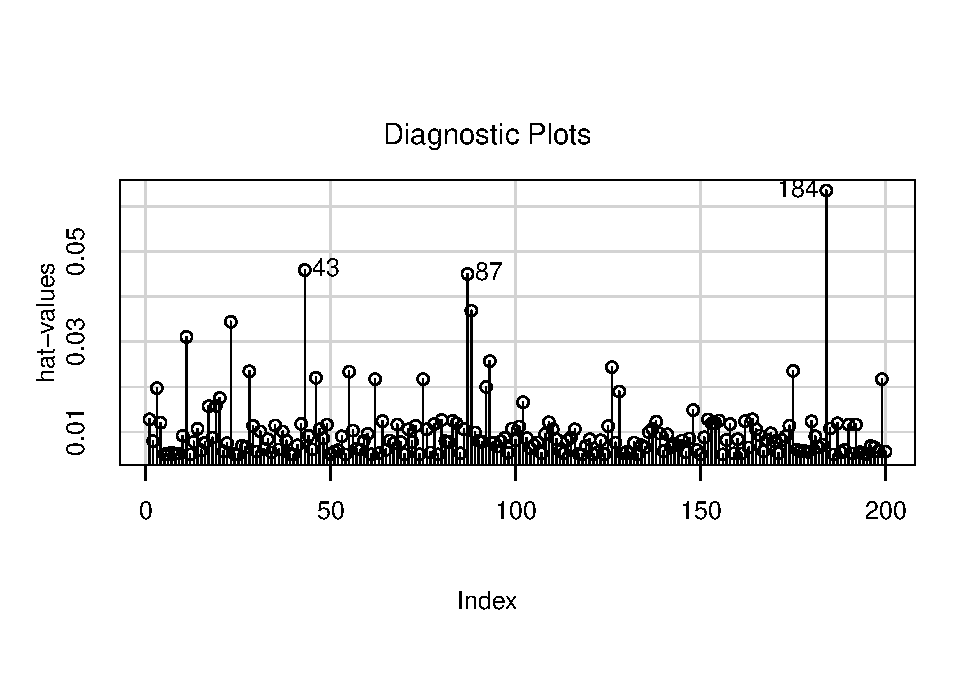
\includegraphics{02_Kap_2_files/figure-latex/unnamed-chunk-67-1.pdf}

Det som i grafen over kalles ``hat values'' er et vanlig mål for å finne observasjoner/caser som er relativt langt fra senter av prediksjonsrommet og som derfor \textbf{potensielt} har stor innflytelse på OLS-regresjonskoeffisientene (``leverage'') \citep{foxCompanionAppliedRegression2019}. \citet{huberRobustStatistics1981} anbefaler følgende grenseverdier: verdier under \(0.2\) er ønskelig, verdier over \(0.5\) uønskede, og verdier mellom \(0.2\) og \(0.5\) problematiske.

``Hat values'' er altså et mål på potensiell innflytelse. Neste mål - \emph{DfBetas} - er et mål på observasjonens effekt på regresjonskoeffisinenten for hver variabel med og uten den innflytelsesrike observasjonen - eller med andre ord: observasjonenes innflytelse på variablene. \citet{belsleyRegressionDiagnosticsIdentifying1980} anbefaler 2 som cut-off verdi for å indikere innflytelsesrike observasjoner.

\begin{Shaded}
\begin{Highlighting}[]
\CommentTok{\# Bruker pakken: olsrr}
\FunctionTok{ols\_plot\_dfbetas}\NormalTok{(FieldOLS\_reg, }\AttributeTok{print\_plot =} \ConstantTok{TRUE}\NormalTok{)}
\end{Highlighting}
\end{Shaded}

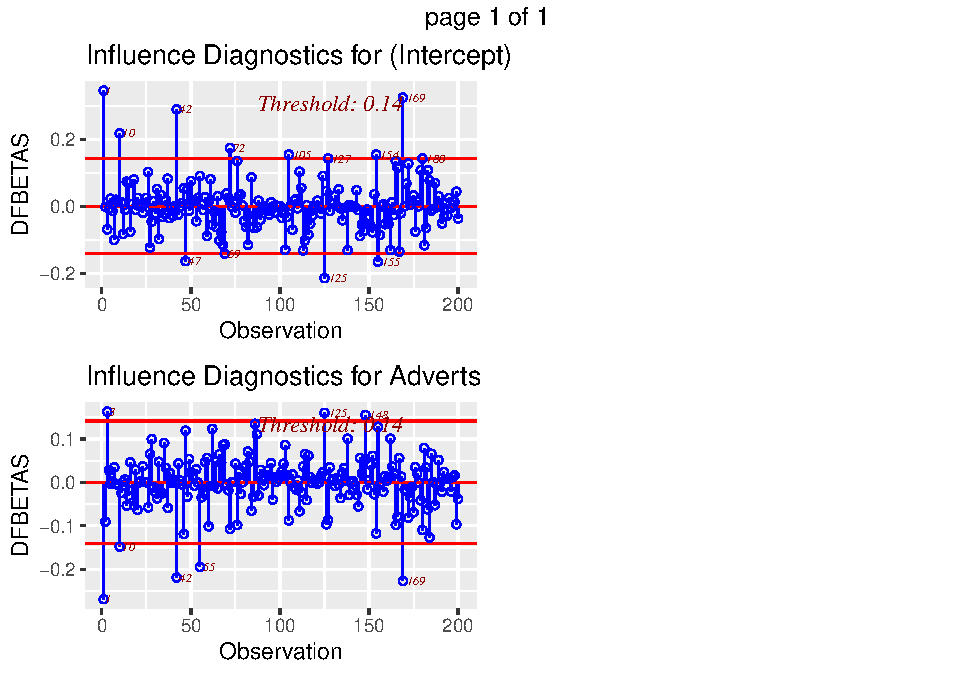
\includegraphics{02_Kap_2_files/figure-latex/unnamed-chunk-68-1.pdf}

Pakken legger automatisk inn cutoff-verdi (i dette tilfellet 0.14). Formelen for utregning av dfbeta cutoff-verdi er \(\frac{2}{\sqrt{n}}\), der n=antall observasjoner.

Vi kan også se på \emph{dffit} \citep{welschLinearRegressionDiagnostics1977}.

\begin{Shaded}
\begin{Highlighting}[]
\CommentTok{\# Bruker pakken: olsrr}
\FunctionTok{ols\_plot\_dffits}\NormalTok{(FieldOLS\_reg)}
\end{Highlighting}
\end{Shaded}

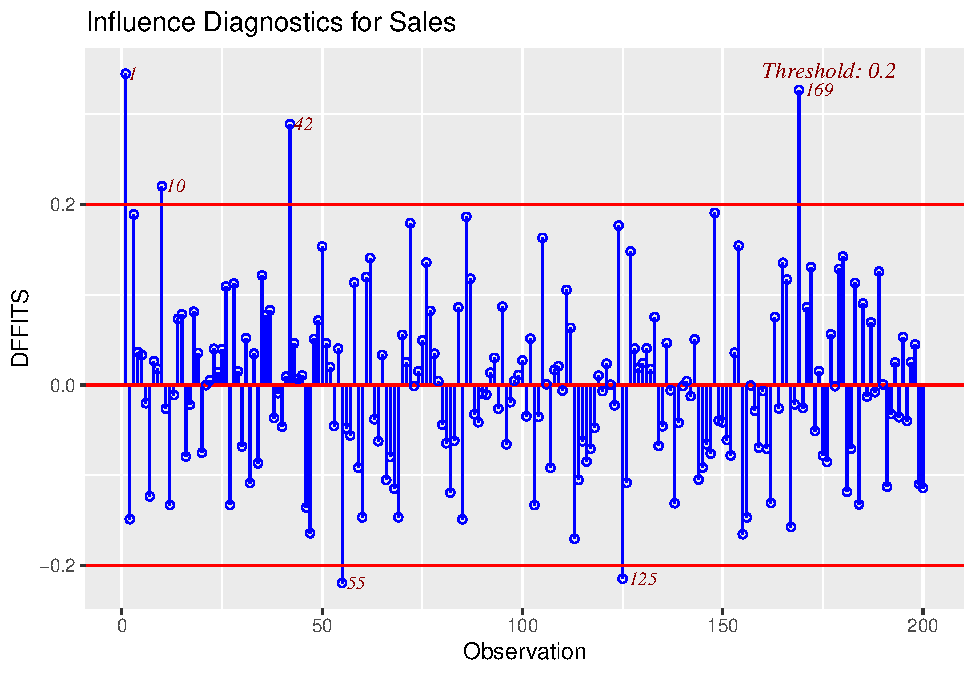
\includegraphics{02_Kap_2_files/figure-latex/unnamed-chunk-69-1.pdf}

Cutoff-verdi i dette tilfellet er 0.2. Formel for utregning er \(2*\frac{\sqrt{(k+1)}}{(n-k-1)}\), der k = antall prediktorer og n = antall observasjoner.

Det siste målet vi ønsker å se på (og trolig den mest brukte) er ``Cook's distance'', som gir et mål på observasjonens totale innflytelse på regresjonsmodellen.

\begin{Shaded}
\begin{Highlighting}[]
\CommentTok{\# Bruker pakken: car}
\FunctionTok{influenceIndexPlot}\NormalTok{(FieldOLS\_reg, }\AttributeTok{vars =} \StringTok{"Cook"}\NormalTok{, }\AttributeTok{id =} \FunctionTok{list}\NormalTok{(}\AttributeTok{n=}\DecValTok{3}\NormalTok{))}
\end{Highlighting}
\end{Shaded}

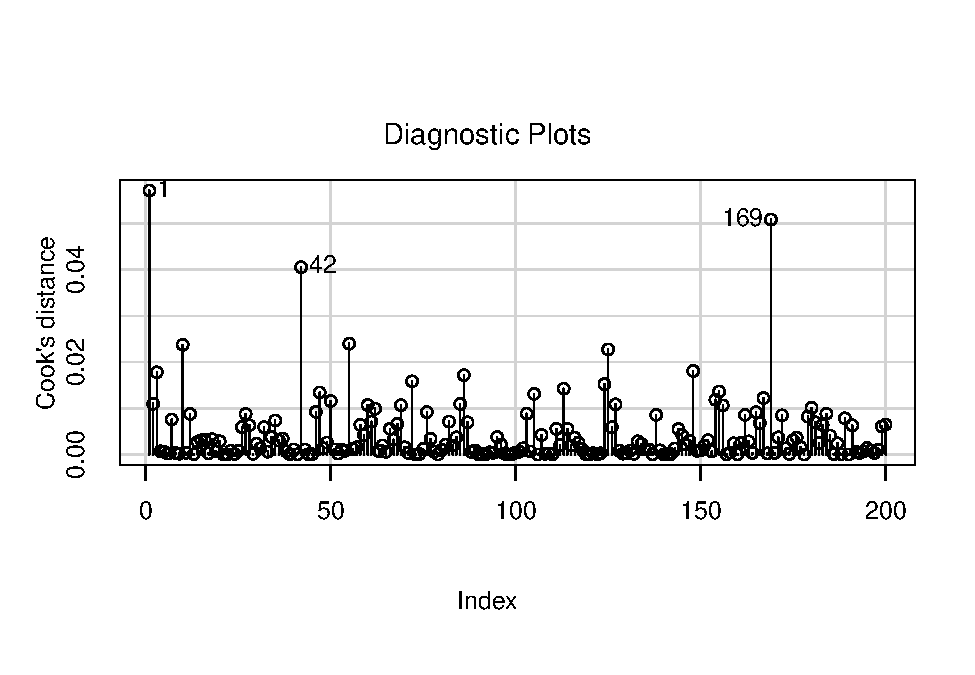
\includegraphics{02_Kap_2_files/figure-latex/unnamed-chunk-70-1.pdf}

I grafen over vises Cook's distance - et mål på vektet kvadratsum for forskjellene mellom de individuelle elementene til koeffisienten. Sagt på en annen måte: Vi bruker Cook's distance til å se hvilke observasjoner/caser som kan påvirke modellen vår uforholdsmessig mye (totalt sett). Dersom vi har mange caser med høy verdi på Cook's distance kan det være en indikasjon på at lineær regresjon kanskje ikke er en egnet analyse for det foreliggende datasettet.

Så hva er høy verdi på Cook's distance? Kilder som \citet{cookResidualsInfluenceRegression1982} og \citet{tabachnikUsingMultivariateStatistics2007} angir at verdier over 1 er bekymringsfullt. Andre, som \citet{foxRegressionDiagnosticsIntroduction2020}, advarer mot en ren numerisk vurdering (og fremhever viktigheten av både grafisk presentasjon og vurdering av hvert enkelt tilfelle). En tilnærming som er anbefalt (se f.eks. \citet{zachHowIdentifyInfluential2019}) er å bruker forholdstallet \(4/N\) - i vårt tilfelle \(4/200=0.02\).

La oss hente opp Cook's distance for de største verdiene for de enkelte observasjoner:

\begin{Shaded}
\begin{Highlighting}[]
\CommentTok{\# Base R}
\NormalTok{mineCDverdier }\OtherTok{\textless{}{-}} \FunctionTok{cooks.distance}\NormalTok{(FieldOLS\_reg)}
\NormalTok{mineCDverdier }\OtherTok{\textless{}{-}} \FunctionTok{round}\NormalTok{(mineCDverdier, }\DecValTok{3}\NormalTok{)}
\FunctionTok{head}\NormalTok{(}\FunctionTok{sort}\NormalTok{(mineCDverdier, }\AttributeTok{decreasing =} \ConstantTok{TRUE}\NormalTok{), }\AttributeTok{n =} \DecValTok{10}\NormalTok{)}
\CommentTok{\#\textgreater{}     1   169    42    10    55   125     3   148    86    72 }
\CommentTok{\#\textgreater{} 0.057 0.051 0.041 0.024 0.024 0.023 0.018 0.018 0.017 0.016}
\end{Highlighting}
\end{Shaded}

Her kjenner vi igjen observasjonene 1, 169 og 42 som de med høyest verdi på Cook's distance, men også casene 10, 55 og 125 har verdier over anbefalingen som kommer fra \(4/n\). Men vi ser også at verdien er relativt lave hvis man tar utgangspunkt i 1 som bekymringsfullt. For å vise eventuell justering av modellen som følge av uteliggere viser vi likevel framgangsmåte.

Vi bør også undersøke ``added variable plots'' - i en regresjon kan observasjonene ha både en individuell og en sammensatt/felles påvirkning.

\begin{Shaded}
\begin{Highlighting}[]
\CommentTok{\# Bruker pakken: car}
\FunctionTok{avPlots}\NormalTok{(FieldOLS\_reg, }\AttributeTok{id=}\FunctionTok{list}\NormalTok{(}\AttributeTok{cex=}\FloatTok{0.75}\NormalTok{, }\AttributeTok{n=}\DecValTok{3}\NormalTok{, }\AttributeTok{method=}\StringTok{"mahal"}\NormalTok{))}
\end{Highlighting}
\end{Shaded}

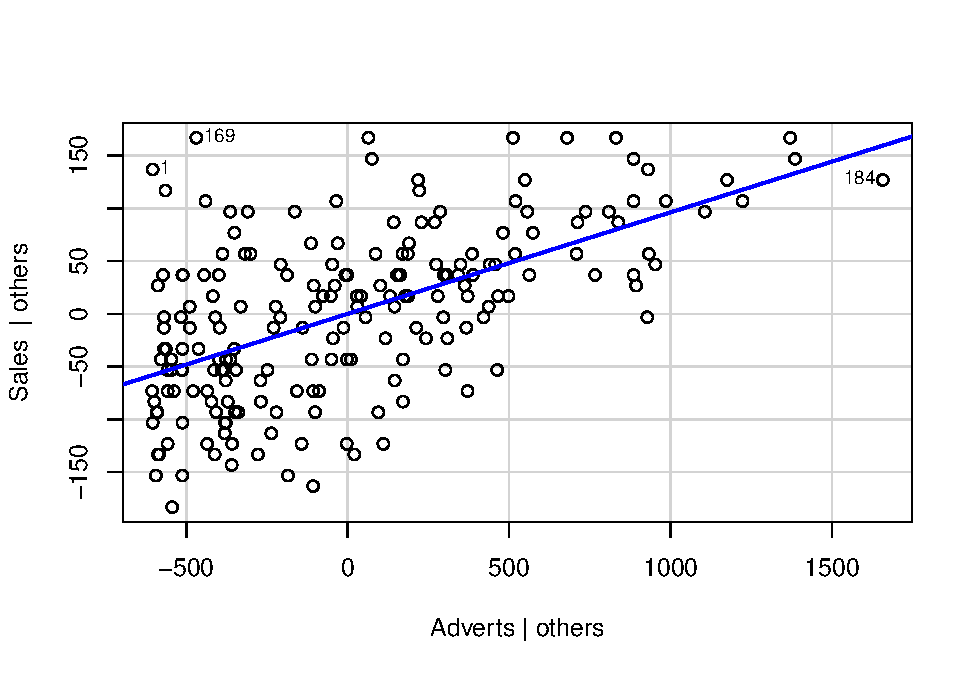
\includegraphics{02_Kap_2_files/figure-latex/unnamed-chunk-72-1.pdf}

Her sier \citet{foxCompanionAppliedRegression2019}, s.44 at ``Points at the extreme left or right of the plot correspond to cases that have high leverage on the corresponding coefficients and consequenlty are potentially influential''.

\hypertarget{steg-6-eventuell-revisjon-av-modell}{%
\subsubsection{Steg 6: Eventuell revisjon av modell}\label{steg-6-eventuell-revisjon-av-modell}}

Her kan vi for eksempel se hvordan modellens presterer ved bortfall av visse ekstreme verdier (spesielt innflytelsesrike observasjoner/caser, jfr. diskusjon under regresjonsforutsetnigner) eller ved inkludering/eksklusjon av gitte variabler i modellen (først og fremst ved multippel regresjonsanalyse).

Vi bør vurdere punktene over og vurdere om vi ønsker å lage en revidert modell der vi tar ut veldig innflytelsesrike caser/observasjoner. Som tidligere nevnt har vi ikke svært store verdier her, men la oss som et eksempel si at vi ønsker å se om en modell uten observasjon 169. Vi anbefaler å ta bort en og en observasjon siden (som nevnt) observasjonene/casene har både en individuell og felles påvirkning.

\begin{Shaded}
\begin{Highlighting}[]
\NormalTok{FieldOLS\_reg2 }\OtherTok{\textless{}{-}} \FunctionTok{update}\NormalTok{(FieldOLS\_reg, }\AttributeTok{subset =} \SpecialCharTok{{-}}\DecValTok{169}\NormalTok{)}
\CommentTok{\# Bruker pakken: car}
\FunctionTok{compareCoefs}\NormalTok{(FieldOLS\_reg, FieldOLS\_reg2)}
\CommentTok{\#\textgreater{} Calls:}
\CommentTok{\#\textgreater{} 1: lm(formula = Sales \textasciitilde{} Adverts, data = Field\_OLS\_data)}
\CommentTok{\#\textgreater{} 2: lm(formula = Sales \textasciitilde{} Adverts, data = Field\_OLS\_data, }
\CommentTok{\#\textgreater{}   subset = {-}169)}
\CommentTok{\#\textgreater{} }
\CommentTok{\#\textgreater{}             Model 1 Model 2}
\CommentTok{\#\textgreater{} (Intercept)  134.14  131.76}
\CommentTok{\#\textgreater{} SE             7.54    7.39}
\CommentTok{\#\textgreater{}                            }
\CommentTok{\#\textgreater{} Adverts     0.09612 0.09826}
\CommentTok{\#\textgreater{} SE          0.00963 0.00942}
\CommentTok{\#\textgreater{} }
\end{Highlighting}
\end{Shaded}

Som forventet ser vi ikke de store forskjellene. Vi kan ta bort de andre observasjonene for illustrasjonens skyld:

\begin{Shaded}
\begin{Highlighting}[]
\NormalTok{FieldOLS\_reg3 }\OtherTok{\textless{}{-}} \FunctionTok{update}\NormalTok{(FieldOLS\_reg, }\AttributeTok{subset =} \SpecialCharTok{{-}}\FunctionTok{c}\NormalTok{(}\DecValTok{1}\NormalTok{, }\DecValTok{42}\NormalTok{, }\DecValTok{169}\NormalTok{, }\DecValTok{184}\NormalTok{))}
\FunctionTok{compareCoefs}\NormalTok{(FieldOLS\_reg, FieldOLS\_reg2, FieldOLS\_reg3)}
\CommentTok{\#\textgreater{} Calls:}
\CommentTok{\#\textgreater{} 1: lm(formula = Sales \textasciitilde{} Adverts, data = Field\_OLS\_data)}
\CommentTok{\#\textgreater{} 2: lm(formula = Sales \textasciitilde{} Adverts, data = Field\_OLS\_data, }
\CommentTok{\#\textgreater{}   subset = {-}169)}
\CommentTok{\#\textgreater{} 3: lm(formula = Sales \textasciitilde{} Adverts, data = Field\_OLS\_data, }
\CommentTok{\#\textgreater{}   subset = {-}c(1, 42, 169, 184))}
\CommentTok{\#\textgreater{} }
\CommentTok{\#\textgreater{}             Model 1 Model 2 Model 3}
\CommentTok{\#\textgreater{} (Intercept)  134.14  131.76  126.14}
\CommentTok{\#\textgreater{} SE             7.54    7.39    7.28}
\CommentTok{\#\textgreater{}                                    }
\CommentTok{\#\textgreater{} Adverts     0.09612 0.09826 0.10461}
\CommentTok{\#\textgreater{} SE          0.00963 0.00942 0.00942}
\CommentTok{\#\textgreater{} }
\end{Highlighting}
\end{Shaded}

Igjen, ikke de store endringene. Vi kan se at Intercept (\(\beta\)) går litt ned etter hvert som vi tar bort caser, og betydningen av Adverts går litt opp (men det er marginalt).

La oss, for eksempelets skyld, manipulere datasettet slik at en analyse av Cook's distance ser slik ut:

\begin{Shaded}
\begin{Highlighting}[]
\CommentTok{\# Bruker pakken: readxl}
\NormalTok{Field\_OLS\_data2 }\OtherTok{\textless{}{-}} \FunctionTok{read\_excel}\NormalTok{(}\StringTok{"Field\_datasett\_OLS2.xlsx"}\NormalTok{)}
\CommentTok{\# Base R}
\NormalTok{FieldOLS\_man }\OtherTok{\textless{}{-}} \FunctionTok{lm}\NormalTok{(}\AttributeTok{formula =}\NormalTok{ Sales }\SpecialCharTok{\textasciitilde{}}\NormalTok{ Adverts, }\AttributeTok{data =}\NormalTok{ Field\_OLS\_data2)}
\CommentTok{\# Bruker pakken: car}
\FunctionTok{influenceIndexPlot}\NormalTok{(FieldOLS\_man, }\AttributeTok{vars =} \FunctionTok{c}\NormalTok{(}\StringTok{"Cook"}\NormalTok{), }\AttributeTok{id =} \FunctionTok{list}\NormalTok{(}\AttributeTok{n=}\DecValTok{3}\NormalTok{))}
\end{Highlighting}
\end{Shaded}

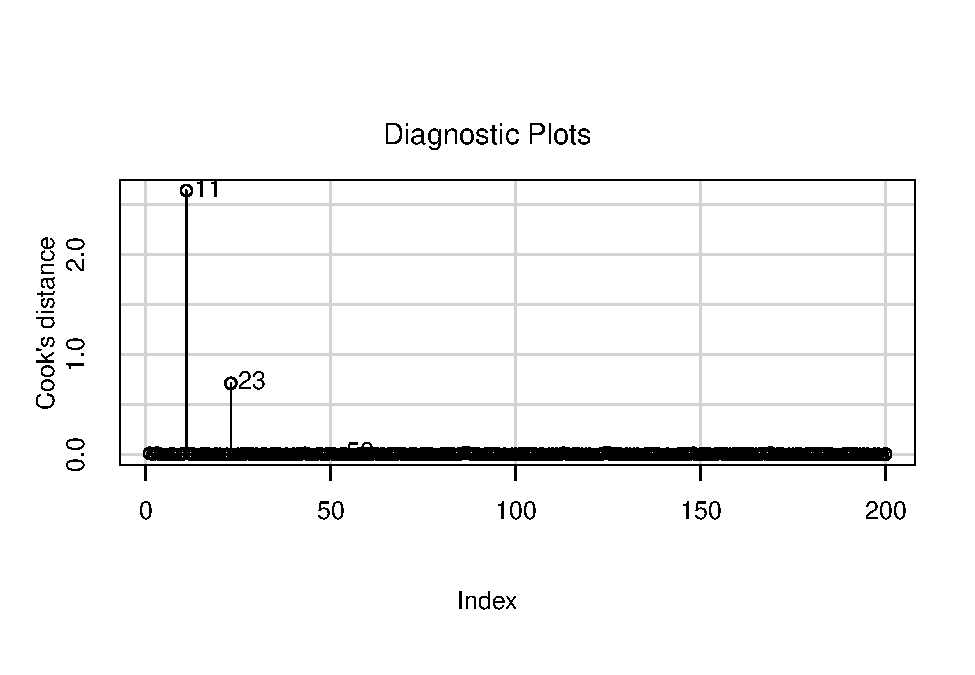
\includegraphics{02_Kap_2_files/figure-latex/unnamed-chunk-75-1.pdf}

Hvis vi nå kjører denne modellen opp mot en modell der vi tar bort 11 og 23 får vi:

\begin{Shaded}
\begin{Highlighting}[]
\NormalTok{FieldOLS\_man2 }\OtherTok{\textless{}{-}} \FunctionTok{update}\NormalTok{(FieldOLS\_man, }\AttributeTok{subset =} \SpecialCharTok{{-}}\FunctionTok{c}\NormalTok{(}\DecValTok{11}\NormalTok{, }\DecValTok{23}\NormalTok{))}
\CommentTok{\# Bruker pakken: car}
\FunctionTok{compareCoefs}\NormalTok{(FieldOLS\_man, FieldOLS\_man2)}
\CommentTok{\#\textgreater{} Calls:}
\CommentTok{\#\textgreater{} 1: lm(formula = Sales \textasciitilde{} Adverts, data = Field\_OLS\_data2)}
\CommentTok{\#\textgreater{} 2: lm(formula = Sales \textasciitilde{} Adverts, data = Field\_OLS\_data2,}
\CommentTok{\#\textgreater{}    subset = {-}c(11, 23))}
\CommentTok{\#\textgreater{} }
\CommentTok{\#\textgreater{}             Model 1 Model 2}
\CommentTok{\#\textgreater{} (Intercept)  183.77  134.14}
\CommentTok{\#\textgreater{} SE             5.97    7.64}
\CommentTok{\#\textgreater{}                            }
\CommentTok{\#\textgreater{} Adverts     0.01207 0.09621}
\CommentTok{\#\textgreater{} SE          0.00298 0.00999}
\CommentTok{\#\textgreater{} }
\end{Highlighting}
\end{Shaded}

Her ser vi koeffisienten for Adverts stiger fra 0.01 til 0.09, eller en endring på 11.1\%.

\hypertarget{steg-7-eventuell-analyse-av-revidert-modell}{%
\subsubsection{Steg 7: Eventuell analyse av revidert modell}\label{steg-7-eventuell-analyse-av-revidert-modell}}

Her vil vi prinsippet bare gjenta samme analyser som ved analyse av den opprinnelige modellen.

\hypertarget{steg-8-konklusjon-oppsummering-rapportering-av-resultater}{%
\subsubsection{Steg 8: Konklusjon / oppsummering / rapportering av resultater}\label{steg-8-konklusjon-oppsummering-rapportering-av-resultater}}

Tabell 1: Deskriptiv statistikk

\begin{Shaded}
\begin{Highlighting}[]
\CommentTok{\# Bruker pakken: table1}
\NormalTok{table1}\SpecialCharTok{::}\FunctionTok{label}\NormalTok{(Field\_OLS\_data}\SpecialCharTok{$}\NormalTok{Adverts) }\OtherTok{\textless{}{-}} \StringTok{"Adverts"}
\NormalTok{table1}\SpecialCharTok{::}\FunctionTok{label}\NormalTok{(Field\_OLS\_data}\SpecialCharTok{$}\NormalTok{Sales) }\OtherTok{\textless{}{-}} \StringTok{"Sales"}
\NormalTok{table1}\SpecialCharTok{::}\FunctionTok{table1}\NormalTok{(}\SpecialCharTok{\textasciitilde{}}\NormalTok{Adverts }\SpecialCharTok{+}\NormalTok{ Sales, }\AttributeTok{data =}\NormalTok{ Field\_OLS\_data)}
\end{Highlighting}
\end{Shaded}

\begin{tabular}[t]{ll}
\toprule
  & Overall\\
\midrule
 & (N=200)\\
\addlinespace[0.3em]
\multicolumn{2}{l}{\textbf{Adverts}}\\
\hspace{1em}Mean (SD) & 614 (486)\\
\hspace{1em}Median [Min, Max] & 532 [9.10, 2270]\\
\addlinespace[0.3em]
\multicolumn{2}{l}{\textbf{Sales}}\\
\hspace{1em}Mean (SD) & 193 (80.7)\\
\hspace{1em}Median [Min, Max] & 200 [10.0, 360]\\
\bottomrule
\end{tabular}

Tabell 2: Korrelasjonsmatrise

\begin{Shaded}
\begin{Highlighting}[]
\CommentTok{\# Bruker pakken: sjPlot}
\NormalTok{FieldOLSkorr }\OtherTok{\textless{}{-}} \FunctionTok{tab\_corr}\NormalTok{(Field\_OLS\_data, }\AttributeTok{triangle =} \StringTok{"lower"}\NormalTok{)}
\NormalTok{FieldOLSkorr}
\end{Highlighting}
\end{Shaded}

~

Adverts

Sales

Airplay

Image

Adverts

~

~

~

~

Sales

0.578***

~

~

~

Airplay

0.102{}

0.599***

~

~

Image

0.081{}

0.326***

0.182**

~

Computed correlation used pearson-method with listwise-deletion.

p \textless{} .0001**** , p \textless{} .001*** , p \textless{} .01**, p \textless{} .05*

Tabell 3: Hierarkisk regresjonsanalyse av prediktorer for totalt selvoppfattet stress (tpstress)

\begin{Shaded}
\begin{Highlighting}[]
\CommentTok{\# Bruker pakken: sjPlot}
\FunctionTok{tab\_model}\NormalTok{(FieldOLS\_reg)}
\end{Highlighting}
\end{Shaded}

~

Sales

Predictors

Estimates

CI

p

(Intercept)

134.14

119.28~--~149.00

\textless0.001

Adverts

0.10

0.08~--~0.12

\textless0.001

Observations

200

R2 / R2 adjusted

0.335 / 0.331

Vi viser her rapportering av en enkel lineær regresjonsanalyse etter APA-standard:

En enkel lineær regresjon ble gjennomført for å predikere salgstall per uke basert på sum brukt på reklame uka før lansering. Vi fant en signifikant regresjonslikning (F(1,198) = 99.59, \(\beta\) = 134.14p \textless{} .001) med en \(R^2\) på .335, 95\% CI {[}119.28, 149.00{]}.

\hypertarget{til-slutt-for-r-brukere}{%
\subsubsection{Til slutt for R-brukere\ldots{}}\label{til-slutt-for-r-brukere}}

\citet{mehmetogluInnforingStatistiskeDataanalyser2020} har skrevet en veldig god bok om på norsk: ``Innføring i R for statistiske analyser'' som vi varmt kan anbefale. Den kommer med en pakke (``rnorsk'') som kan lastes ned gjennom kommandoen \textbf{devtools::install\_github(``ihrke/rnorsk'')} (forutsetter at pakken ``devtools'' er på plass, hvis ikke så kjør ``package.install(''devtools'')).

Forfatterne har laget en samling av regresjonsdiagnostikk som vi viser her på Fields data der vi laget en multippel regresjonsmodell:

\begin{Shaded}
\begin{Highlighting}[]
\FunctionTok{options}\NormalTok{(}\AttributeTok{scipen=}\DecValTok{999}\NormalTok{)}
\CommentTok{\# Bruker pakken: rnorsk}
\FunctionTok{regression.diagnostics}\NormalTok{(FieldOLS\_mult\_reg)}
\CommentTok{\#\textgreater{} Tests of linear model assumptions}
\CommentTok{\#\textgreater{} {-}{-}{-}{-}{-}{-}{-}{-}{-}{-}{-}{-}{-}{-}{-}{-}{-}{-}{-}{-}{-}{-}{-}{-}{-}{-}{-}{-}{-}{-}{-}{-}{-}}
\CommentTok{\#\textgreater{} }
\CommentTok{\#\textgreater{} 1/11 (9.1 \%) checks failed}
\CommentTok{\#\textgreater{} }
\CommentTok{\#\textgreater{} }
\CommentTok{\#\textgreater{} Identified problems: }
\CommentTok{\#\textgreater{}  functional form}
\CommentTok{\#\textgreater{} Summary:}
\CommentTok{\#\textgreater{} \# A tibble: 11 x 8}
\CommentTok{\#\textgreater{}    assumption variable test  statistic p.value  crit problem}
\CommentTok{\#\textgreater{}    \textless{}chr\textgreater{}      \textless{}chr\textgreater{}    \textless{}chr\textgreater{}     \textless{}dbl\textgreater{}   \textless{}dbl\textgreater{} \textless{}dbl\textgreater{} \textless{}chr\textgreater{}  }
\CommentTok{\#\textgreater{}  1 heteroske\textasciitilde{} global   stud\textasciitilde{}   6.19e+0  0.103   0.05 No Pro\textasciitilde{}}
\CommentTok{\#\textgreater{}  2 heteroske\textasciitilde{} global   Non{-}\textasciitilde{}   3.03e{-}1  0.582   0.05 No Pro\textasciitilde{}}
\CommentTok{\#\textgreater{}  3 multicoll\textasciitilde{} Adverts  Vari\textasciitilde{}   1.01e+0 NA       5    No Pro\textasciitilde{}}
\CommentTok{\#\textgreater{}  4 multicoll\textasciitilde{} Airplay  Vari\textasciitilde{}   1.04e+0 NA       5    No Pro\textasciitilde{}}
\CommentTok{\#\textgreater{}  5 multicoll\textasciitilde{} Image    Vari\textasciitilde{}   1.04e+0 NA       5    No Pro\textasciitilde{}}
\CommentTok{\#\textgreater{}  6 normality  global   Shap\textasciitilde{}   9.95e{-}1  0.725   0.01 No Pro\textasciitilde{}}
\CommentTok{\#\textgreater{}  7 model spe\textasciitilde{} global   Stat\textasciitilde{}  {-}6.99e{-}5  0.916   0.05 No Pro\textasciitilde{}}
\CommentTok{\#\textgreater{}  8 functiona\textasciitilde{} global   RESE\textasciitilde{}   3.72e+0  0.0261  0.05 Problem}
\CommentTok{\#\textgreater{}  9 outliers   global   Cook\textasciitilde{}   7.08e{-}2 NA       1    No Pro\textasciitilde{}}
\CommentTok{\#\textgreater{} 10 outliers   global   Bonf\textasciitilde{}   3.16e+0  0.362   0.05 No Pro\textasciitilde{}}
\CommentTok{\#\textgreater{} 11 autocorre\textasciitilde{} global   Durb\textasciitilde{}   2.70e{-}3  0.814   0.05 No Pro\textasciitilde{}}
\CommentTok{\#\textgreater{} \# ... with 1 more variable: decision \textless{}chr\textgreater{}}
\CommentTok{\#\textgreater{} }
\CommentTok{\#\textgreater{} Outliers:}
\CommentTok{\#\textgreater{} {-}{-}{-}{-}{-}{-}{-}{-}{-}{-}{-}}
\CommentTok{\#\textgreater{} Cook\textquotesingle{}s distance (criterion=1.00): No outliers}
\CommentTok{\#\textgreater{} Outlier test (criterion=0.05): No outliers}
\end{Highlighting}
\end{Shaded}

Analysen gir en samlet oversikt over et antall parametere og søker å hjelpe til med beslutning om forutsetninger er ok/ikke ok, men vi vil understreke at kunnskap om hva som ligger bak de ulike testene og kriteriene er essensielt. Mer informasjon om parameterene finner dere \href{https://ihrke.github.io/rnorsk/reference/regression.diagnostics.html}{her}.

\hypertarget{standard-multippel-regresjonsanalyse}{%
\subsection{Standard multippel regresjonsanalyse}\label{standard-multippel-regresjonsanalyse}}

\hypertarget{eksempel-standard-multippel-regresjonsanalyse}{%
\subsubsection{Eksempel standard multippel regresjonsanalyse}\label{eksempel-standard-multippel-regresjonsanalyse}}

Vi skal i gå gjennom et eksempel på multippel regresjonsanalyse, ved å følge stegene under.

\begin{enumerate}
\def\labelenumi{\arabic{enumi}.}
\item
  Analyse av dataene
\item
  Evtentuelt valg av prediktorer ut fra analyse av dataene
\item
  Lage modell (kjøre regresjonsanalysen)
\item
  Analyse av resultatene (diagnostikk)
\item
  Sjekk av forutsetningene
\item
  Eventuell revisjon av modellen
\item
  Eventuell analyse av revidert modell
\item
  Konklusjon / oppsummering / rapportering av resultater
\end{enumerate}

\hypertarget{analyse-av-dataene}{%
\subsubsection{Analyse av dataene}\label{analyse-av-dataene}}

Vi skal bruke et datasett fra \citet{pallantSPSSSurvivalManual2010} som du kan finne \href{https://www.mheducation.co.uk/data-files}{her}.

\begin{Shaded}
\begin{Highlighting}[]
\CommentTok{\# Base R}
\CommentTok{\# Bruker pakken: readxl}
\NormalTok{Pallant\_survey }\OtherTok{\textless{}{-}} \FunctionTok{as.data.frame}\NormalTok{(}\FunctionTok{read\_excel}\NormalTok{(}\StringTok{"Pallant\_survey.xlsx"}\NormalTok{))}
\end{Highlighting}
\end{Shaded}

Datasettet er for stort til å vises fram i sin helhet, men vi skal bruke to uavhengige variabler - tmast (Control of external events) og tpcioss (Control of internal states) mot den avhengige variabelen tpstress (Perceived stress).

Vi ønsker altså å se om en gruppe studenters (N = 439) egenrapporterte oppfattelse av sin kontroll over eksterne forhold som kan skape stress og deres evne til å kontrollere deres følelser, tanker og fysiske reaksjoner \citep{pallantDevelopmentValidationScale2000}. Vi kan derfor se nærmere på variablene.

\begin{Shaded}
\begin{Highlighting}[]
\CommentTok{\# Base R}
\NormalTok{Pallant\_survey2 }\OtherTok{\textless{}{-}} \FunctionTok{select}\NormalTok{(Pallant\_survey, tmast, tpcoiss, tpstress)}
\NormalTok{Pallant\_survey2 }\OtherTok{\textless{}{-}} \FunctionTok{na.omit}\NormalTok{(Pallant\_survey2) }
\CommentTok{\# Bruker pakken: summarytools}
\NormalTok{summarytools}\SpecialCharTok{::}\FunctionTok{descr}\NormalTok{(Pallant\_survey2, }\AttributeTok{stats =} \StringTok{"common"}\NormalTok{)}
\CommentTok{\#\textgreater{} Descriptive Statistics  }
\CommentTok{\#\textgreater{} Pallant\_survey2  }
\CommentTok{\#\textgreater{} N: 426  }
\CommentTok{\#\textgreater{} }
\CommentTok{\#\textgreater{}                    tmast   tpcoiss   tpstress}
\CommentTok{\#\textgreater{} {-}{-}{-}{-}{-}{-}{-}{-}{-}{-}{-}{-}{-}{-}{-} {-}{-}{-}{-}{-}{-}{-}{-} {-}{-}{-}{-}{-}{-}{-}{-}{-} {-}{-}{-}{-}{-}{-}{-}{-}{-}{-}}
\CommentTok{\#\textgreater{}            Mean    21.74     60.56      26.75}
\CommentTok{\#\textgreater{}         Std.Dev     3.97     11.96       5.84}
\CommentTok{\#\textgreater{}             Min     8.00     20.00      12.00}
\CommentTok{\#\textgreater{}          Median    22.00     62.00      26.00}
\CommentTok{\#\textgreater{}             Max    28.00     88.00      46.00}
\CommentTok{\#\textgreater{}         N.Valid   426.00    426.00     426.00}
\CommentTok{\#\textgreater{}       Pct.Valid   100.00    100.00     100.00}
\end{Highlighting}
\end{Shaded}

\begin{Shaded}
\begin{Highlighting}[]
\CommentTok{\# Base R}
\FunctionTok{par}\NormalTok{(}\AttributeTok{mfrow=}\NormalTok{(}\FunctionTok{c}\NormalTok{(}\DecValTok{2}\NormalTok{,}\DecValTok{2}\NormalTok{)))}
\NormalTok{histtmast }\OtherTok{\textless{}{-}} \FunctionTok{with}\NormalTok{(Pallant\_survey2, }\FunctionTok{hist}\NormalTok{(tmast))}
\NormalTok{histtpcoiss }\OtherTok{\textless{}{-}} \FunctionTok{with}\NormalTok{(Pallant\_survey2, }\FunctionTok{hist}\NormalTok{(tpcoiss))}
\NormalTok{histtpstress }\OtherTok{\textless{}{-}} \FunctionTok{with}\NormalTok{(Pallant\_survey2, }\FunctionTok{hist}\NormalTok{(tpstress))}
\end{Highlighting}
\end{Shaded}

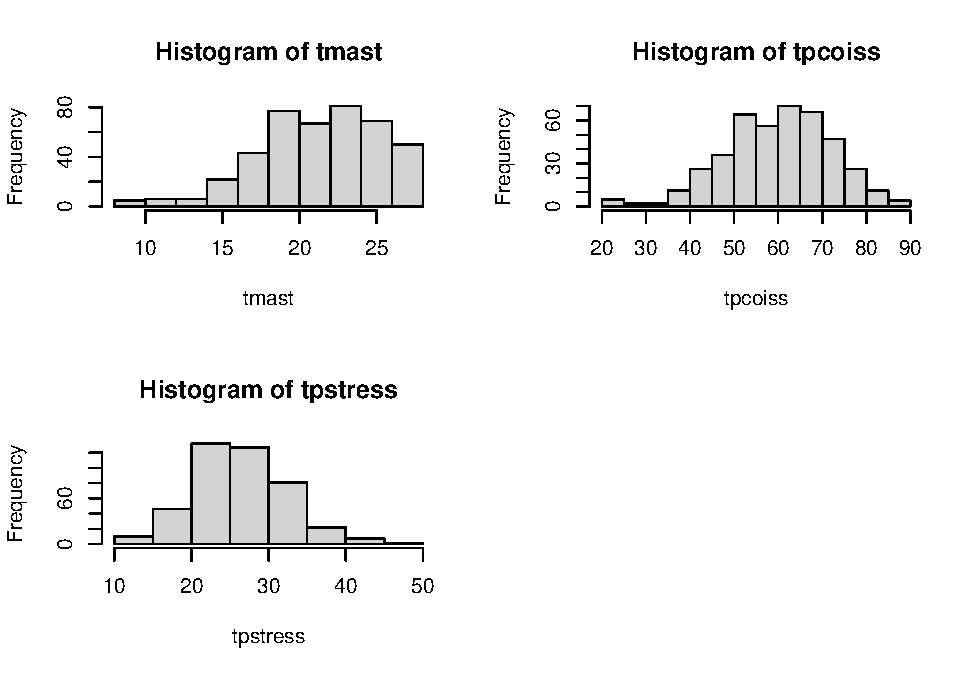
\includegraphics{02_Kap_2_files/figure-latex/unnamed-chunk-86-1.pdf}

\begin{Shaded}
\begin{Highlighting}[]
\CommentTok{\# Bruker pakken: car}
\NormalTok{qqtmast }\OtherTok{\textless{}{-}}\NormalTok{ car}\SpecialCharTok{::}\FunctionTok{qqPlot}\NormalTok{(}\SpecialCharTok{\textasciitilde{}}\NormalTok{ tmast, }\AttributeTok{data =}\NormalTok{ Pallant\_survey2)}
\end{Highlighting}
\end{Shaded}

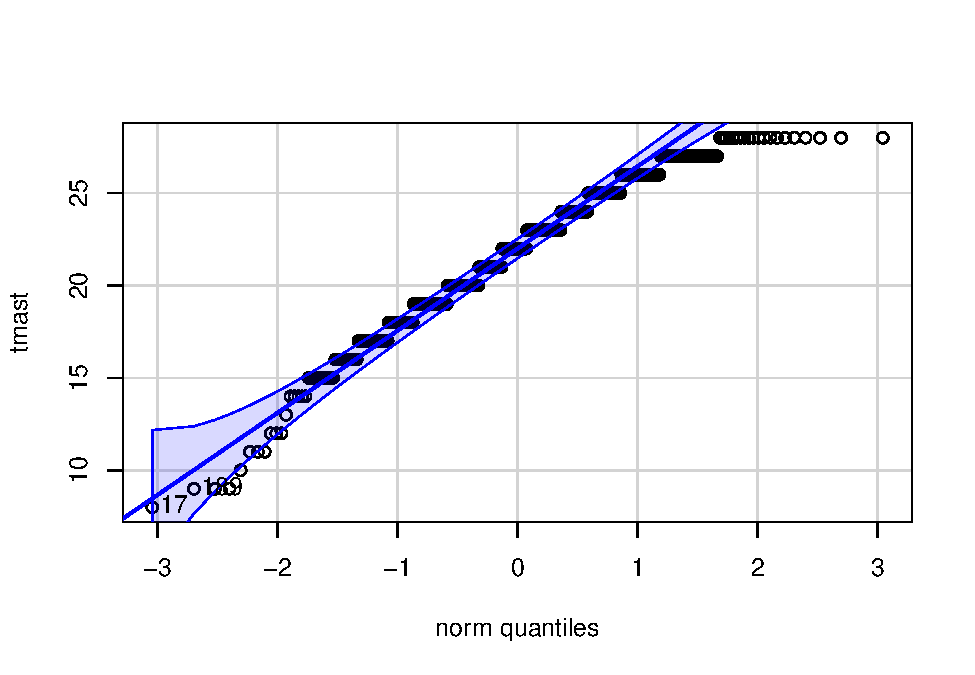
\includegraphics{02_Kap_2_files/figure-latex/unnamed-chunk-87-1.pdf}

\begin{Shaded}
\begin{Highlighting}[]
\NormalTok{qqtpcoiss }\OtherTok{\textless{}{-}}\NormalTok{ car}\SpecialCharTok{::}\FunctionTok{qqPlot}\NormalTok{(}\SpecialCharTok{\textasciitilde{}}\NormalTok{ tpcoiss, }\AttributeTok{data =}\NormalTok{ Pallant\_survey2)}
\end{Highlighting}
\end{Shaded}

\includegraphics{02_Kap_2_files/figure-latex/unnamed-chunk-87-2.pdf}

\begin{Shaded}
\begin{Highlighting}[]
\NormalTok{qqtpstress }\OtherTok{\textless{}{-}}\NormalTok{ car}\SpecialCharTok{::}\FunctionTok{qqPlot}\NormalTok{(}\SpecialCharTok{\textasciitilde{}}\NormalTok{ tpstress, }\AttributeTok{data =}\NormalTok{ Pallant\_survey2)}
\end{Highlighting}
\end{Shaded}

\includegraphics{02_Kap_2_files/figure-latex/unnamed-chunk-87-3.pdf}

\begin{Shaded}
\begin{Highlighting}[]
\CommentTok{\# Base R}
\FunctionTok{boxplot}\NormalTok{(Pallant\_survey2)}
\end{Highlighting}
\end{Shaded}

\includegraphics{02_Kap_2_files/figure-latex/unnamed-chunk-88-1.pdf}

\hypertarget{evtentuelt-valg-av-prediktorer-ut-fra-analyse-av-dataene}{%
\subsubsection{Evtentuelt valg av prediktorer ut fra analyse av dataene}\label{evtentuelt-valg-av-prediktorer-ut-fra-analyse-av-dataene}}

Vi gjør ingen analyse av dette da vi har valgt to uavhengige variabler ut fra eksempelet til \citet{pallantSPSSSurvivalManual2010}.

\hypertarget{lage-modell-kjuxf8re-regresjonsanalysen}{%
\subsubsection{Lage modell (kjøre regresjonsanalysen)}\label{lage-modell-kjuxf8re-regresjonsanalysen}}

\includegraphics[width=0.5\textwidth,height=\textheight]{PallantOLS.png}

\hypertarget{analyse-av-resultatene-diagnostikk}{%
\subsubsection{Analyse av resultatene (diagnostikk)}\label{analyse-av-resultatene-diagnostikk}}

\hypertarget{antall-prediktoreruavhengige-variabler-overfitting-og-predicted-r-square}{%
\paragraph{Antall prediktorer/uavhengige variabler, overfitting og predicted R-square}\label{antall-prediktoreruavhengige-variabler-overfitting-og-predicted-r-square}}

I multippel regresjonsanalyse har vi mer enn en prediktor/uavhengig variabel. Som regel kan vi ønske å inkludere mer enn en prediktor fordi vi sjeldent klarer å fange nok av variansen i en avhengig variabel gjennom en prediktor. Samtidig ønsker vi ikke flere uavhengige variabler enn nødvendig for å lage en så enkel modell som mulig som gir oss prediksjoner vi kan bruke. Matematisk er det også slik at enhver uavhengig variabel som har en grad av korrelasjon med den avhengige variabelen vil bidra til å øke \(R^2\) uten at det nødvendigvis gjør modellen ``riktigere'' (men kan gjøre den vanskeligere å tolke). Dersom vi legger til unødvendige uavhengige variabler risikerer vi det som kalles overfitting - altså at modellen blir god på å beskrive tilfeldige feil i dataene heller enn å beskrive forholdet mellom variablene. Resultatet er at modellen ikke kan generaliseres. Vi kan også se tilbake på regresjonsforutsetningene og vil se at et stort antall uavhengige variabler er en invitasjon til multikolinearitet.

En måte å sjekke dette er å dele datasettet slik at man gjør regresjonsanalysen på en del av datasettet og deretter tester modellen på den andre delen av datasettet. Dette kalles kryssvalidering. En annen måte er å se på ``predicted R-square'' som innebærer følgende prosedyre (som statistikkprogrammer gjør for oss naturligvis):

\begin{itemize}
\tightlist
\item
  Et datapunkt/observasjon tas ut av datasettet
\item
  Regresjonslikningen kalkuleres
\item
  Modellens evne til å predikere det datapunktet/observasjonen som ble tatt ut evalueres (altså - hvor nærme datapunktet kommer vår modell i sin prediksjon?)
\item
  Dette gjentas for alle datapunktene i datasettet
\end{itemize}

Tolkningen av dette er ganske grei. Man sammenlikner R-square med predicted R-square. Dersom det er liten forskjell mellom disse verdiene har man trolig liten sannsynlighet for at du har overfitting av modellen. Dersom forskjellen er stor er det grunn til å tro at man kan ha overfitting.

For å unngå dette er det viktig å tenke på forholdstallene som ble diskutert under foregående punkt om regresjonsforutsetninger. Kjennskap til tidligere forskning og resultater vil gi informasjon om og et teoretisk grunnlag for hvilke variabler som bør inkluderes i modellen.

Vi skal illustrere overfitting basert på et eksempel fra \citet{frostHowInterpretAdjusted2022} (dette eksempelet har altså ikke noe direkte med analysen vi er inne i - Pallant sitt datasett - men er tatt med for å illustrere poenget med \emph{overfitting}).

\begin{Shaded}
\begin{Highlighting}[]
\CommentTok{\# Base R}
\NormalTok{PresidentRanking }\OtherTok{\textless{}{-}} \FunctionTok{read.csv}\NormalTok{(}\StringTok{"PresidentRanking.csv"}\NormalTok{)}

\CommentTok{\# Bruker pakken: summarytools}
\NormalTok{summarytools}\SpecialCharTok{::}\FunctionTok{descr}\NormalTok{(PresidentRanking)}
\CommentTok{\#\textgreater{} Descriptive Statistics  }
\CommentTok{\#\textgreater{} PresidentRanking  }
\CommentTok{\#\textgreater{} N: 12  }
\CommentTok{\#\textgreater{} }
\CommentTok{\#\textgreater{}                     Approval.High   Historians.rank}
\CommentTok{\#\textgreater{} {-}{-}{-}{-}{-}{-}{-}{-}{-}{-}{-}{-}{-}{-}{-}{-}{-} {-}{-}{-}{-}{-}{-}{-}{-}{-}{-}{-}{-}{-}{-}{-} {-}{-}{-}{-}{-}{-}{-}{-}{-}{-}{-}{-}{-}{-}{-}{-}{-}}
\CommentTok{\#\textgreater{}              Mean           78.75             17.00}
\CommentTok{\#\textgreater{}           Std.Dev            8.01             10.90}
\CommentTok{\#\textgreater{}               Min           67.00              2.00}
\CommentTok{\#\textgreater{}                Q1           72.00              8.50}
\CommentTok{\#\textgreater{}            Median           79.00             15.00}
\CommentTok{\#\textgreater{}                Q3           85.50             25.00}
\CommentTok{\#\textgreater{}               Max           90.00             38.00}
\CommentTok{\#\textgreater{}               MAD           10.38             11.86}
\CommentTok{\#\textgreater{}               IQR           12.25             15.75}
\CommentTok{\#\textgreater{}                CV            0.10              0.64}
\CommentTok{\#\textgreater{}          Skewness           {-}0.05              0.37}
\CommentTok{\#\textgreater{}       SE.Skewness            0.64              0.64}
\CommentTok{\#\textgreater{}          Kurtosis           {-}1.58             {-}1.20}
\CommentTok{\#\textgreater{}           N.Valid           12.00             12.00}
\CommentTok{\#\textgreater{}         Pct.Valid          100.00            100.00}
\end{Highlighting}
\end{Shaded}

Datasettet inneholder to variabler: Hvordan historikere rangerer amerikanske presidenter (Historians.rank) og hvor stor generell støtte presidenter har hatt i befolkningen (Approval.High).

\begin{Shaded}
\begin{Highlighting}[]
\CommentTok{\# Base R}
\NormalTok{presidentlm }\OtherTok{\textless{}{-}} \FunctionTok{lm}\NormalTok{(}\AttributeTok{formula =}\NormalTok{ Historians.rank }\SpecialCharTok{\textasciitilde{}}\NormalTok{ Approval.High, }\AttributeTok{data =}\NormalTok{ PresidentRanking)}
\FunctionTok{plot}\NormalTok{(Historians.rank }\SpecialCharTok{\textasciitilde{}}\NormalTok{ Approval.High, }\AttributeTok{data =}\NormalTok{ PresidentRanking)}
\FunctionTok{abline}\NormalTok{(presidentlm, }\AttributeTok{lwd =} \DecValTok{2}\NormalTok{, }\AttributeTok{col =} \StringTok{"red"}\NormalTok{)}
\end{Highlighting}
\end{Shaded}

\includegraphics{02_Kap_2_files/figure-latex/unnamed-chunk-90-1.pdf}

\begin{Shaded}
\begin{Highlighting}[]
\FunctionTok{summ}\NormalTok{(presidentlm)}
\end{Highlighting}
\end{Shaded}

\begin{table}[!h]
\centering
\begin{tabular}{lr}
\toprule
\cellcolor{gray!6}{Observations} & \cellcolor{gray!6}{12}\\
Dependent variable & Historians.rank\\
\cellcolor{gray!6}{Type} & \cellcolor{gray!6}{OLS linear regression}\\
\bottomrule
\end{tabular}
\end{table} \begin{table}[!h]
\centering
\begin{tabular}{lr}
\toprule
\cellcolor{gray!6}{F(1,10)} & \cellcolor{gray!6}{0.07}\\
R² & 0.01\\
\cellcolor{gray!6}{Adj. R²} & \cellcolor{gray!6}{-0.09}\\
\bottomrule
\end{tabular}
\end{table} \begin{table}[!h]
\centering
\begin{threeparttable}
\begin{tabular}{lrrrr}
\toprule
  & Est. & S.E. & t val. & p\\
\midrule
\cellcolor{gray!6}{(Intercept)} & \cellcolor{gray!6}{25.81} & \cellcolor{gray!6}{33.91} & \cellcolor{gray!6}{0.76} & \cellcolor{gray!6}{0.46}\\
Approval.High & -0.11 & 0.43 & -0.26 & 0.80\\
\bottomrule
\end{tabular}
\begin{tablenotes}
\item Standard errors: OLS
\end{tablenotes}
\end{threeparttable}
\end{table}

Vi ser at R-squared er \(0.0068\) - hvilket vi vil tolke som at det i praksis ikke er noen sammenheng mellom variablene.

Vi kan så bruke en polynomisk likning (her har vi brukt \(x^3\) for å lage regresjonslinjen):

\begin{Shaded}
\begin{Highlighting}[]
\CommentTok{\# Base R}
\NormalTok{presidentlm2 }\OtherTok{\textless{}{-}} \FunctionTok{lm}\NormalTok{(Historians.rank }\SpecialCharTok{\textasciitilde{}} \FunctionTok{poly}\NormalTok{(Approval.High, }\AttributeTok{degree=}\DecValTok{3}\NormalTok{), }\AttributeTok{data=}\NormalTok{PresidentRanking)}
\CommentTok{\# Bruker pakken: ggplot2}
\FunctionTok{ggplot}\NormalTok{(}\AttributeTok{data=}\NormalTok{PresidentRanking, }\FunctionTok{aes}\NormalTok{(Approval.High,Historians.rank)) }\SpecialCharTok{+}
    \FunctionTok{geom\_point}\NormalTok{() }\SpecialCharTok{+} 
    \FunctionTok{geom\_smooth}\NormalTok{(}\AttributeTok{method=}\StringTok{"lm"}\NormalTok{, }\AttributeTok{formula=}\NormalTok{y}\SpecialCharTok{\textasciitilde{}}\FunctionTok{I}\NormalTok{(x}\SpecialCharTok{\^{}}\DecValTok{3}\NormalTok{)}\SpecialCharTok{+}\FunctionTok{I}\NormalTok{(x}\SpecialCharTok{\^{}}\DecValTok{2}\NormalTok{))}
\end{Highlighting}
\end{Shaded}

\includegraphics{02_Kap_2_files/figure-latex/unnamed-chunk-91-1.pdf}

\begin{Shaded}
\begin{Highlighting}[]
\FunctionTok{summ}\NormalTok{(presidentlm2)}
\end{Highlighting}
\end{Shaded}

\begin{table}[!h]
\centering
\begin{tabular}{lr}
\toprule
\cellcolor{gray!6}{Observations} & \cellcolor{gray!6}{12}\\
Dependent variable & Historians.rank\\
\cellcolor{gray!6}{Type} & \cellcolor{gray!6}{OLS linear regression}\\
\bottomrule
\end{tabular}
\end{table} \begin{table}[!h]
\centering
\begin{tabular}{lr}
\toprule
\cellcolor{gray!6}{F(3,8)} & \cellcolor{gray!6}{5.27}\\
R² & 0.66\\
\cellcolor{gray!6}{Adj. R²} & \cellcolor{gray!6}{0.54}\\
\bottomrule
\end{tabular}
\end{table} \begin{table}[!h]
\centering
\begin{threeparttable}
\begin{tabular}{lrrrr}
\toprule
  & Est. & S.E. & t val. & p\\
\midrule
\cellcolor{gray!6}{(Intercept)} & \cellcolor{gray!6}{17.00} & \cellcolor{gray!6}{2.14} & \cellcolor{gray!6}{7.95} & \cellcolor{gray!6}{0.00}\\
poly(Approval.High, degree = 3)1 & -2.97 & 7.41 & -0.40 & 0.70\\
\cellcolor{gray!6}{poly(Approval.High, degree = 3)2} & \cellcolor{gray!6}{19.41} & \cellcolor{gray!6}{7.41} & \cellcolor{gray!6}{2.62} & \cellcolor{gray!6}{0.03}\\
poly(Approval.High, degree = 3)3 & 21.94 & 7.41 & 2.96 & 0.02\\
\bottomrule
\end{tabular}
\begin{tablenotes}
\item Standard errors: OLS
\end{tablenotes}
\end{threeparttable}
\end{table}

Vi har nå en R-squared på \(0.66\) for denne modellen mot \(0.0068\) for den lineære modellen. Dette betyr at den polynomiske regresjonsmodellen forklarer drøye 66\% av variansen i den avhengige variabelen. Modellen vår er ut fra dette en god modell for våre data.
Imidlertid gir en analyse av Predicted R-square oss et annet bilde av modellen:

\begin{Shaded}
\begin{Highlighting}[]
\CommentTok{\# Bruker pakken: olsrr}
\FunctionTok{ols\_pred\_rsq}\NormalTok{(presidentlm2)}
\CommentTok{\#\textgreater{} [1] {-}0.2162257}
\end{Highlighting}
\end{Shaded}

I realiteten forteller både verdien på predicted r-square på 0, og forskjellen mellom R-square (\(0.664\)) og predicted R-square \(0\), at vi har en seriøs overfitting. Vi har med andre ord funnet en modell som beskriver dataene våre veldig godt, men som ikke kan brukes på andre data enn de vi har (vel, den kan jo brukes, men vil ikke kunne gi oss noe av verdi). Vi kan altså ikke predikere noe ut fra modellen.

\begin{Shaded}
\begin{Highlighting}[]
\CommentTok{\# Bruker pakken: summarytools}
\NormalTok{PallantOLS\_reg }\OtherTok{\textless{}{-}} \FunctionTok{lm}\NormalTok{(tpstress }\SpecialCharTok{\textasciitilde{}}\NormalTok{ tmast }\SpecialCharTok{+}\NormalTok{ tpcoiss, }\AttributeTok{data =}\NormalTok{ Pallant\_survey2)}
\FunctionTok{summ}\NormalTok{(PallantOLS\_reg)}
\end{Highlighting}
\end{Shaded}

\begin{table}[!h]
\centering
\begin{tabular}{lr}
\toprule
\cellcolor{gray!6}{Observations} & \cellcolor{gray!6}{426}\\
Dependent variable & tpstress\\
\cellcolor{gray!6}{Type} & \cellcolor{gray!6}{OLS linear regression}\\
\bottomrule
\end{tabular}
\end{table} \begin{table}[!h]
\centering
\begin{tabular}{lr}
\toprule
\cellcolor{gray!6}{F(2,423)} & \cellcolor{gray!6}{184.49}\\
R² & 0.47\\
\cellcolor{gray!6}{Adj. R²} & \cellcolor{gray!6}{0.46}\\
\bottomrule
\end{tabular}
\end{table} \begin{table}[!h]
\centering
\begin{threeparttable}
\begin{tabular}{lrrrr}
\toprule
  & Est. & S.E. & t val. & p\\
\midrule
\cellcolor{gray!6}{(Intercept)} & \cellcolor{gray!6}{50.83} & \cellcolor{gray!6}{1.27} & \cellcolor{gray!6}{40.00} & \cellcolor{gray!6}{0.00}\\
tmast & -0.62 & 0.06 & -10.10 & 0.00\\
\cellcolor{gray!6}{tpcoiss} & \cellcolor{gray!6}{-0.17} & \cellcolor{gray!6}{0.02} & \cellcolor{gray!6}{-8.56} & \cellcolor{gray!6}{0.00}\\
\bottomrule
\end{tabular}
\begin{tablenotes}
\item Standard errors: OLS
\end{tablenotes}
\end{threeparttable}
\end{table}

Vi ser at \(R^2 = 0.466\). Modellen kan altså forklare \(46.6%
\) av variansen i den avhengige variabelen. Vi ser at vi får en noe lavere verdi for «Adjusted R Squared» i forhold til «R Squared». Når vi legger til en uavhengig variabel i en regresjonsanalyse er det lite sannsynlig at korrelasjonen mellom den nye uavhengige variabelen og den avhengige variabelen vil være nøyaktig 0. Den vil i stedet fluktuere rundt 0. Pga. denne tilfeldige fluktuasjonen rundt 0 vil \(R^2\) alltid øke litt når man legger til en ny uavhengig variabel. Adjusted \(R^2\) søker å kompensere for dette å få fram en mer korrekt verdi. Jo større antall uavhengige variabler, jo større forskjell vil man se mellom \(R^2\) og Adjusted \(R^2\). Det samme vil være tilfelle ved mindre utvalgsstørrelser fordi variasjonen rundt 0 vil være større i mindre utvalg.

Vi kan også legge merke til at Predicted R-Squared er \(0.456\) og dermed svært lik R-squared.

\hypertarget{modellens-koeffisienter}{%
\paragraph{Modellens koeffisienter}\label{modellens-koeffisienter}}

Vi ser først på tallene for ``Std.Beta'' under ``Parameter Estimated''. Vi ser at tmast bidrar i større grad enn tpcoiss (fortegn er i denne sammenheng irrelevant). Begge bidrar signifikant.

\hypertarget{hvor-god-er-modellen-vuxe5r-goodness-of-fit-1}{%
\paragraph{Hvor god er modellen vår (goodness of fit)?}\label{hvor-god-er-modellen-vuxe5r-goodness-of-fit-1}}

Vi kan se at F-verdien er 184.5. Vi kan regne ut (bruke R) til å finne kritiske verdi.

\begin{Shaded}
\begin{Highlighting}[]
\CommentTok{\# Base R}
\FunctionTok{qf}\NormalTok{(}\AttributeTok{p=}\NormalTok{.}\DecValTok{05}\NormalTok{, }\AttributeTok{df1=}\DecValTok{2}\NormalTok{, }\AttributeTok{df2=}\DecValTok{423}\NormalTok{, }\AttributeTok{lower.tail=}\ConstantTok{FALSE}\NormalTok{)}
\CommentTok{\#\textgreater{} [1] 3.017049}
\end{Highlighting}
\end{Shaded}

F-verdien er dermed langt over kritisk verdi (p \textless{} 0.001).

Det ser derfor ut til at det er svært usannsynlig at forbedringen fra referansemodellen (gjennomsnittet) til vår modell er tilfeldig. Vi kan også si at dersom forbedringen ved regresjonsmodellen er større enn unøyaktigheten i modellen så vil F \textgreater{} 1.

\hypertarget{sjekk-av-forutsetningene}{%
\subsubsection{Sjekk av forutsetningene}\label{sjekk-av-forutsetningene}}

Vi viser resultater av tester og grafer, men diskuterer ikke disse nærmere. I stedet viser vi til gjennomgangen av forutsetningene lenger opp .

\hypertarget{kausalitet-1}{%
\paragraph{Kausalitet}\label{kausalitet-1}}

Vi antar at det foreligger godt teoretisk grunnlag for modellen.

\hypertarget{variablene-er-uten-muxe5lefeil-1}{%
\paragraph{Variablene er uten målefeil}\label{variablene-er-uten-muxe5lefeil-1}}

Vi må forutsette at vi ikke har systematiske målefeil i variablene.

\hypertarget{relevante-og-irrelevante-variabler-1}{%
\paragraph{Relevante og irrelevante variabler}\label{relevante-og-irrelevante-variabler-1}}

Også dette forutsetter vi er på plass.

\hypertarget{forholdstall-mellom-caserobservasjoner-og-uavhengige-variabler-1}{%
\paragraph{Forholdstall mellom caser/observasjoner og uavhengige variabler}\label{forholdstall-mellom-caserobservasjoner-og-uavhengige-variabler-1}}

\begin{Shaded}
\begin{Highlighting}[]
\CommentTok{\# Base R}
\FunctionTok{nrow}\NormalTok{(Pallant\_survey2)}
\CommentTok{\#\textgreater{} [1] 426}
\end{Highlighting}
\end{Shaded}

Vi har altså 426 observasjoner. I forhold til tabellen vist under forutsetninger lenger opp tilfredsstiller dette godt de ulike måtene å betrakte forholdstallet vi har vist til.

\hypertarget{de-uavhengige-variablene-er-additiv-for-den-avhengige-variabelen-1}{%
\paragraph{De uavhengige variablene er additiv for den avhengige variabelen}\label{de-uavhengige-variablene-er-additiv-for-den-avhengige-variabelen-1}}

Vi kan mistenke at det kan være en interaksjon mellom variablene tmast og tpcoiss - jo større kontroll på eksterne hendelser, jo større er kontrollen over følelser, tanker og fysisker reaksjoner. Vi ser derfor etter en interaksjonseffekt.

\begin{Shaded}
\begin{Highlighting}[]
\CommentTok{\# Base R}
\NormalTok{PallantOLS\_reg2 }\OtherTok{\textless{}{-}} \FunctionTok{lm}\NormalTok{(tpstress }\SpecialCharTok{\textasciitilde{}}\NormalTok{ tmast }\SpecialCharTok{+}\NormalTok{ tpcoiss, Pallant\_survey2)}
\NormalTok{PallantOLS\_inter }\OtherTok{\textless{}{-}} \FunctionTok{lm}\NormalTok{(tpstress }\SpecialCharTok{\textasciitilde{}}\NormalTok{.}\SpecialCharTok{+}\NormalTok{tmast}\SpecialCharTok{*}\NormalTok{tpcoiss, Pallant\_survey2)}
\CommentTok{\# Bruker pakken: car}
\FunctionTok{compareCoefs}\NormalTok{(PallantOLS\_reg2, PallantOLS\_inter)}
\CommentTok{\#\textgreater{} Calls:}
\CommentTok{\#\textgreater{} 1: lm(formula = tpstress \textasciitilde{} tmast + tpcoiss, data = }
\CommentTok{\#\textgreater{}   Pallant\_survey2)}
\CommentTok{\#\textgreater{} 2: lm(formula = tpstress \textasciitilde{} . + tmast * tpcoiss, data = }
\CommentTok{\#\textgreater{}   Pallant\_survey2)}
\CommentTok{\#\textgreater{} }
\CommentTok{\#\textgreater{}               Model 1 Model 2}
\CommentTok{\#\textgreater{} (Intercept)     50.83   52.66}
\CommentTok{\#\textgreater{} SE               1.27    4.34}
\CommentTok{\#\textgreater{}                              }
\CommentTok{\#\textgreater{} tmast         {-}0.6207 {-}0.7093}
\CommentTok{\#\textgreater{} SE             0.0614  0.2103}
\CommentTok{\#\textgreater{}                              }
\CommentTok{\#\textgreater{} tpcoiss       {-}0.1747 {-}0.2071}
\CommentTok{\#\textgreater{} SE             0.0204  0.0763}
\CommentTok{\#\textgreater{}                              }
\CommentTok{\#\textgreater{} tmast:tpcoiss         0.00154}
\CommentTok{\#\textgreater{} SE                    0.00348}
\CommentTok{\#\textgreater{} }
\end{Highlighting}
\end{Shaded}

Forskjellen mellom modellene ligger altså i den nederste koeffisienten (tmast:tpcoiss) som da er den kombinerte og samtidige effekten av de to variablene. Vi ser at effekten er veldig liten, men grafisk kan vi også se interaksjonseffekten:

\begin{Shaded}
\begin{Highlighting}[]
\CommentTok{\# Bruker pakken: ggplot2}
\FunctionTok{ggplot}\NormalTok{(}\AttributeTok{data=}\NormalTok{Pallant\_survey2, }\FunctionTok{aes}\NormalTok{(}\AttributeTok{x=}\NormalTok{tmast, }\AttributeTok{y=}\NormalTok{tpstress, }\AttributeTok{group=}\DecValTok{1}\NormalTok{)) }\SpecialCharTok{+}\FunctionTok{geom\_smooth}\NormalTok{(}\AttributeTok{method=}\NormalTok{lm,}\AttributeTok{se=}\NormalTok{F)}\SpecialCharTok{+} 
    \FunctionTok{geom\_smooth}\NormalTok{(}\FunctionTok{aes}\NormalTok{(tmast,tpcoiss), }\AttributeTok{method=}\NormalTok{lm, }\AttributeTok{se=}\NormalTok{F,}\AttributeTok{color=}\StringTok{"black"}\NormalTok{)}\SpecialCharTok{+}\FunctionTok{xlab}\NormalTok{(}\StringTok{"tmast og tpcoiss"}\NormalTok{)}\SpecialCharTok{+}\FunctionTok{labs}\NormalTok{(}
        \AttributeTok{title=}\StringTok{"tmast i blått {-} tpcoiss i svart"}\NormalTok{)}
\CommentTok{\#\textgreater{} \textasciigrave{}geom\_smooth()\textasciigrave{} using formula \textquotesingle{}y \textasciitilde{} x\textquotesingle{}}
\CommentTok{\#\textgreater{} \textasciigrave{}geom\_smooth()\textasciigrave{} using formula \textquotesingle{}y \textasciitilde{} x\textquotesingle{}}
\end{Highlighting}
\end{Shaded}

\includegraphics{02_Kap_2_files/figure-latex/unnamed-chunk-97-1.pdf}

Det kan se ut som en interaksjonseffekt ved at linjene ikke er parallelle. Det kan imidlertid være noe vanskelig å tolke interaksjonseffekt. Man kan f.eks. ha en interaksjonseffekt som ikke er statistisk signifikant. I R kan vi bruke pakken \emph{jtools} som hjelp:

\begin{Shaded}
\begin{Highlighting}[]
\CommentTok{\# Bruker pakken: jtools}
\FunctionTok{summ}\NormalTok{(PallantOLS\_inter)}
\end{Highlighting}
\end{Shaded}

\begin{table}[!h]
\centering
\begin{tabular}{lr}
\toprule
\cellcolor{gray!6}{Observations} & \cellcolor{gray!6}{426}\\
Dependent variable & tpstress\\
\cellcolor{gray!6}{Type} & \cellcolor{gray!6}{OLS linear regression}\\
\bottomrule
\end{tabular}
\end{table} \begin{table}[!h]
\centering
\begin{tabular}{lr}
\toprule
\cellcolor{gray!6}{F(3,422)} & \cellcolor{gray!6}{122.82}\\
R² & 0.47\\
\cellcolor{gray!6}{Adj. R²} & \cellcolor{gray!6}{0.46}\\
\bottomrule
\end{tabular}
\end{table} \begin{table}[!h]
\centering
\begin{threeparttable}
\begin{tabular}{lrrrr}
\toprule
  & Est. & S.E. & t val. & p\\
\midrule
\cellcolor{gray!6}{(Intercept)} & \cellcolor{gray!6}{52.66} & \cellcolor{gray!6}{4.34} & \cellcolor{gray!6}{12.13} & \cellcolor{gray!6}{0.00}\\
tmast & -0.71 & 0.21 & -3.37 & 0.00\\
\cellcolor{gray!6}{tpcoiss} & \cellcolor{gray!6}{-0.21} & \cellcolor{gray!6}{0.08} & \cellcolor{gray!6}{-2.72} & \cellcolor{gray!6}{0.01}\\
tmast:tpcoiss & 0.00 & 0.00 & 0.44 & 0.66\\
\bottomrule
\end{tabular}
\begin{tablenotes}
\item Standard errors: OLS
\end{tablenotes}
\end{threeparttable}
\end{table}

Vi ser at interaksjonen tmast:tpcoiss ikke er statistisk signifikant.

\begin{Shaded}
\begin{Highlighting}[]
\CommentTok{\# Bruker pakken: interactions}
\FunctionTok{interact\_plot}\NormalTok{(PallantOLS\_inter, }\AttributeTok{pred =}\NormalTok{ tmast, }\AttributeTok{modx =}\NormalTok{ tpcoiss)}
\end{Highlighting}
\end{Shaded}

\includegraphics{02_Kap_2_files/figure-latex/unnamed-chunk-99-1.pdf}

Tolkningen her er ``som før'': Parallelle linjer indikerer fravær av interaksjonseffekt.

\hypertarget{linearitet-1}{%
\paragraph{Linearitet}\label{linearitet-1}}

Vi kan ikke se på samme type scatterplott for sjekk av linearitet som vi gjorde under enkel OLS (på et todimensjonalt plott). Vi kan imidlertid lage ``added variable plots'' \citep{mostellerDataAnalysisRegression1977}.

\begin{Shaded}
\begin{Highlighting}[]
\CommentTok{\# Bruker pakken: olsrr}
\FunctionTok{ols\_plot\_added\_variable}\NormalTok{(PallantOLS\_reg2, }\AttributeTok{print\_plot =} \ConstantTok{TRUE}\NormalTok{)}
\CommentTok{\#\textgreater{} \textasciigrave{}geom\_smooth()\textasciigrave{} using formula \textquotesingle{}y \textasciitilde{} x\textquotesingle{}}
\CommentTok{\#\textgreater{} \textasciigrave{}geom\_smooth()\textasciigrave{} using formula \textquotesingle{}y \textasciitilde{} x\textquotesingle{}}
\end{Highlighting}
\end{Shaded}

\includegraphics{02_Kap_2_files/figure-latex/unnamed-chunk-100-1.pdf}

X-aksene representerer en enkelt uavhengig variabel (per graf ovenfor). Y-aksen = den avhengige variabelen. Den blå linjen viser sammenhengen mellom den uavhengige variabelen og den avhengige variabelen når alle andre uavhengige variabler holdes konstant. Jo sterkere lineær sammenheng i plottene, jo sterkere er den respektive uavhengige variabelens bidrag i modellen.

I vårt tilfelle vil vi nok konkludere med at forutsetningen om linearitet er (nok) oppfylt.

\hypertarget{residualene-skal-vuxe6re-normalfordelte-1}{%
\paragraph{Residualene skal være normalfordelte}\label{residualene-skal-vuxe6re-normalfordelte-1}}

Side vi vet at residualene lagres i modellen og vi kan plotte ut disse:

\begin{Shaded}
\begin{Highlighting}[]
\CommentTok{\# Base R}
\FunctionTok{hist}\NormalTok{(PallantOLS\_reg2}\SpecialCharTok{$}\NormalTok{residuals)}
\end{Highlighting}
\end{Shaded}

\includegraphics{02_Kap_2_files/figure-latex/unnamed-chunk-101-1.pdf}

Vi kan også se på et Q-Q plott og hente ut testverdier for ulike normalitetstester:

\begin{Shaded}
\begin{Highlighting}[]
\CommentTok{\# Bruker pakken: olsrr}
\FunctionTok{ols\_plot\_resid\_qq}\NormalTok{(PallantOLS\_reg2)}
\end{Highlighting}
\end{Shaded}

\includegraphics{02_Kap_2_files/figure-latex/unnamed-chunk-102-1.pdf}

\begin{Shaded}
\begin{Highlighting}[]
\FunctionTok{ols\_test\_normality}\NormalTok{(PallantOLS\_reg2)}
\CommentTok{\#\textgreater{} {-}{-}{-}{-}{-}{-}{-}{-}{-}{-}{-}{-}{-}{-}{-}{-}{-}{-}{-}{-}{-}{-}{-}{-}{-}{-}{-}{-}{-}{-}{-}{-}{-}{-}{-}{-}{-}{-}{-}{-}{-}{-}{-}{-}{-}{-}{-}}
\CommentTok{\#\textgreater{}        Test             Statistic       pvalue  }
\CommentTok{\#\textgreater{} {-}{-}{-}{-}{-}{-}{-}{-}{-}{-}{-}{-}{-}{-}{-}{-}{-}{-}{-}{-}{-}{-}{-}{-}{-}{-}{-}{-}{-}{-}{-}{-}{-}{-}{-}{-}{-}{-}{-}{-}{-}{-}{-}{-}{-}{-}{-}}
\CommentTok{\#\textgreater{} Shapiro{-}Wilk              0.9911         0.0115 }
\CommentTok{\#\textgreater{} Kolmogorov{-}Smirnov        0.0509         0.2197 }
\CommentTok{\#\textgreater{} Cramer{-}von Mises         31.6502         0.0000 }
\CommentTok{\#\textgreater{} Anderson{-}Darling          1.0978         0.0070 }
\CommentTok{\#\textgreater{} {-}{-}{-}{-}{-}{-}{-}{-}{-}{-}{-}{-}{-}{-}{-}{-}{-}{-}{-}{-}{-}{-}{-}{-}{-}{-}{-}{-}{-}{-}{-}{-}{-}{-}{-}{-}{-}{-}{-}{-}{-}{-}{-}{-}{-}{-}{-}}
\end{Highlighting}
\end{Shaded}

Q-Q plottet viser noe avvik.

En hendig graf er også et plott av residualene på y-aksen og ``fitted values'' på x-aksen:

\begin{Shaded}
\begin{Highlighting}[]
\CommentTok{\# Bruker pakken: olsrr}
\FunctionTok{ols\_plot\_resid\_fit}\NormalTok{(PallantOLS\_reg2)}
\end{Highlighting}
\end{Shaded}

\includegraphics{02_Kap_2_files/figure-latex/unnamed-chunk-103-1.pdf}

I forhold til forutsetningen om normalfordelte residualer skal disse være spredd tilfeldig rundt 0.

Sett under ett kan det i dette tilfellet se ut som at residualene er tilnærmet (nok) normalfordeling.

\hypertarget{fravuxe6r-av-multikolinearitet-1}{%
\paragraph{Fravær av multikolinearitet}\label{fravuxe6r-av-multikolinearitet-1}}

Vi kan derfor sjekke for multikolinearitet gjennom å se på en korrelasjonsmatrisen:

\begin{Shaded}
\begin{Highlighting}[]
\CommentTok{\# Base R}
\NormalTok{PallantKorr }\OtherTok{\textless{}{-}} \FunctionTok{cor}\NormalTok{(Pallant\_survey2, }\AttributeTok{method =} \StringTok{"pearson"}\NormalTok{, }\AttributeTok{use=}\StringTok{"pairwise.complete.obs"}\NormalTok{)}
\FunctionTok{round}\NormalTok{(PallantKorr, }\DecValTok{2}\NormalTok{)}
\CommentTok{\#\textgreater{}          tmast tpcoiss tpstress}
\CommentTok{\#\textgreater{} tmast     1.00    0.53    {-}0.61}
\CommentTok{\#\textgreater{} tpcoiss   0.53    1.00    {-}0.58}
\CommentTok{\#\textgreater{} tpstress {-}0.61   {-}0.58     1.00}
\end{Highlighting}
\end{Shaded}

Hvis vi følger \citet{pallantSPSSSurvivalManual2010} ser vi først at alle de to uavhengige variablene korrelerer mellom \(r=0.58\) og \(r=-0.61\) med den avhengige. Den bivariate korrelasjonen mellom de uavhengige variablene er på \(0.53\). Ut fra korrelasjonsmatrisen bør det ikke være grunn til å frykte multikolinearitet.

\begin{Shaded}
\begin{Highlighting}[]
\CommentTok{\# Bruker pakken. olsrr}
\FunctionTok{ols\_vif\_tol}\NormalTok{(PallantOLS\_reg2)}
\CommentTok{\#\textgreater{}   Variables Tolerance      VIF}
\CommentTok{\#\textgreater{} 1     tmast 0.7220785 1.384891}
\CommentTok{\#\textgreater{} 2   tpcoiss 0.7220785 1.384891}
\end{Highlighting}
\end{Shaded}

Det er ingenting som indikerer at vi har multikolinearitet i dataene i denne modellen.

\hypertarget{fravuxe6r-av-heteroskedasisitet-1}{%
\paragraph{Fravær av heteroskedasisitet}\label{fravuxe6r-av-heteroskedasisitet-1}}

Den såkalte White's test vil også kunne være et godt hjelpemiddel:

\begin{Shaded}
\begin{Highlighting}[]
\CommentTok{\# Bruker pakken: lmtestbptest(PallantOLS\_reg2, \textasciitilde{} tmast*tpcoiss + I(tmast\^{}2) + I(tpcoiss\^{}2), data = Pallant\_survey2)}
\end{Highlighting}
\end{Shaded}

Her ser vi at \(p < 0.001\), dvs. vi kan ikke forkaste nullhypotesen = vi har ikke grunn til å konkludere med at vi har heteroskedasisitet i regresjonsmodellen.

\hypertarget{fravuxe6r-av-autokorrelasjon-1}{%
\paragraph{Fravær av autokorrelasjon}\label{fravuxe6r-av-autokorrelasjon-1}}

\begin{Shaded}
\begin{Highlighting}[]
\CommentTok{\# Bruker pakken: car}
\FunctionTok{durbinWatsonTest}\NormalTok{(PallantOLS\_reg2)}
\CommentTok{\#\textgreater{}  lag Autocorrelation D{-}W Statistic p{-}value}
\CommentTok{\#\textgreater{}    1      0.08185218      1.825972   0.078}
\CommentTok{\#\textgreater{}  Alternative hypothesis: rho != 0}
\end{Highlighting}
\end{Shaded}

Her viser verdien \(1.826\) noe som ikke gir grunn til bekymring.

\hypertarget{fravuxe6r-av-innflytelsesrike-observasjonercaser-1}{%
\paragraph{Fravær av innflytelsesrike observasjoner/caser}\label{fravuxe6r-av-innflytelsesrike-observasjonercaser-1}}

Vi så under punktet ``Analyse av dataene'' (se for eksempel Boxplottet av Adverts) at vi har noen observasjoner i modellen som kan defineres som uteliggere. Vi kan identifisere disse gjennom residualene:

\begin{Shaded}
\begin{Highlighting}[]
\CommentTok{\# Bruker pakken: car}
\NormalTok{car}\SpecialCharTok{::}\FunctionTok{qqPlot}\NormalTok{(PallantOLS\_reg2, }\AttributeTok{id =} \FunctionTok{list}\NormalTok{(}\AttributeTok{n=}\DecValTok{3}\NormalTok{))}
\end{Highlighting}
\end{Shaded}

\includegraphics{02_Kap_2_files/figure-latex/unnamed-chunk-108-1.pdf}

\begin{verbatim}
#>  22 194 269 
#>  21 190 263
\end{verbatim}

Vi ser at residualene ligger innenfor 95\% konfidenstintervall. Det er lite ved residualplottet som vekker bekymring.

Vi kan også kjøre analyser som identifiserer betydning/innvirkning (``influential cases''):

\begin{Shaded}
\begin{Highlighting}[]
\CommentTok{\# Bruker pakken: car}
\FunctionTok{influenceIndexPlot}\NormalTok{(PallantOLS\_reg2, }\AttributeTok{vars =} \StringTok{"hat"}\NormalTok{, }\AttributeTok{id =} \FunctionTok{list}\NormalTok{(}\AttributeTok{n=}\DecValTok{3}\NormalTok{))}
\end{Highlighting}
\end{Shaded}

\includegraphics{02_Kap_2_files/figure-latex/unnamed-chunk-109-1.pdf}

DfBetas:

\begin{Shaded}
\begin{Highlighting}[]
\CommentTok{\# Bruker pakken: olsrr}
\FunctionTok{ols\_plot\_dfbetas}\NormalTok{(PallantOLS\_reg2, }\AttributeTok{print\_plot =} \ConstantTok{TRUE}\NormalTok{)}
\end{Highlighting}
\end{Shaded}

\includegraphics{02_Kap_2_files/figure-latex/unnamed-chunk-110-1.pdf}

dffit:

\begin{Shaded}
\begin{Highlighting}[]
\CommentTok{\# Bruker pakken: olsrr}
\FunctionTok{ols\_plot\_dffits}\NormalTok{(PallantOLS\_reg2, }\AttributeTok{print\_plot =} \ConstantTok{TRUE}\NormalTok{)}
\end{Highlighting}
\end{Shaded}

\includegraphics{02_Kap_2_files/figure-latex/unnamed-chunk-111-1.pdf}

Cook's distance:

\begin{Shaded}
\begin{Highlighting}[]
\CommentTok{\# Bruker pakken: car}
\FunctionTok{influenceIndexPlot}\NormalTok{(PallantOLS\_reg2, }\AttributeTok{vars =} \StringTok{"Cook"}\NormalTok{, }\AttributeTok{id =} \FunctionTok{list}\NormalTok{(}\AttributeTok{n=}\DecValTok{3}\NormalTok{))}
\end{Highlighting}
\end{Shaded}

\includegraphics{02_Kap_2_files/figure-latex/unnamed-chunk-112-1.pdf}

\begin{Shaded}
\begin{Highlighting}[]
\CommentTok{\# Base R}
\NormalTok{mineCDverdier2 }\OtherTok{\textless{}{-}} \FunctionTok{cooks.distance}\NormalTok{(PallantOLS\_reg2)}
\NormalTok{mineCDverdier2 }\OtherTok{\textless{}{-}} \FunctionTok{round}\NormalTok{(mineCDverdier2, }\DecValTok{5}\NormalTok{)}
\FunctionTok{head}\NormalTok{(}\FunctionTok{sort}\NormalTok{(mineCDverdier2, }\AttributeTok{decreasing =} \ConstantTok{TRUE}\NormalTok{))}
\CommentTok{\#\textgreater{}      22     268      23     191     413     194 }
\CommentTok{\#\textgreater{} 0.09556 0.05833 0.05434 0.04374 0.03689 0.03601}
\end{Highlighting}
\end{Shaded}

Det er ingenting ved hat values, DfBetas eller Cook's disgance som er bekymringsfullt.

\hypertarget{oppsummert-om-forutsetningerdiagnostikk}{%
\paragraph{Oppsummert om forutsetninger/diagnostikk}\label{oppsummert-om-forutsetningerdiagnostikk}}

\begin{Shaded}
\begin{Highlighting}[]
\FunctionTok{options}\NormalTok{(}\AttributeTok{scipen=}\DecValTok{999}\NormalTok{)}
\CommentTok{\# Bruker pakken: rnorsk}
\FunctionTok{regression.diagnostics}\NormalTok{(PallantOLS\_reg2)}
\CommentTok{\#\textgreater{} Tests of linear model assumptions}
\CommentTok{\#\textgreater{} {-}{-}{-}{-}{-}{-}{-}{-}{-}{-}{-}{-}{-}{-}{-}{-}{-}{-}{-}{-}{-}{-}{-}{-}{-}{-}{-}{-}{-}{-}{-}{-}{-}}
\CommentTok{\#\textgreater{} }
\CommentTok{\#\textgreater{} 0/10 (0.0 \%) checks failed}
\CommentTok{\#\textgreater{} }
\CommentTok{\#\textgreater{} }
\CommentTok{\#\textgreater{} Identified problems: NONE}
\CommentTok{\#\textgreater{} Summary:}
\CommentTok{\#\textgreater{} \# A tibble: 10 x 8}
\CommentTok{\#\textgreater{}    assumption variable test  statistic p.value  crit problem}
\CommentTok{\#\textgreater{}    \textless{}chr\textgreater{}      \textless{}chr\textgreater{}    \textless{}chr\textgreater{}     \textless{}dbl\textgreater{}   \textless{}dbl\textgreater{} \textless{}dbl\textgreater{} \textless{}chr\textgreater{}  }
\CommentTok{\#\textgreater{}  1 heteroske\textasciitilde{} global   stud\textasciitilde{}   3.95     0.139   0.05 No Pro\textasciitilde{}}
\CommentTok{\#\textgreater{}  2 heteroske\textasciitilde{} global   Non{-}\textasciitilde{}   2.91     0.0881  0.05 No Pro\textasciitilde{}}
\CommentTok{\#\textgreater{}  3 multicoll\textasciitilde{} tmast    Vari\textasciitilde{}   1.38    NA       5    No Pro\textasciitilde{}}
\CommentTok{\#\textgreater{}  4 multicoll\textasciitilde{} tpcoiss  Vari\textasciitilde{}   1.38    NA       5    No Pro\textasciitilde{}}
\CommentTok{\#\textgreater{}  5 normality  global   Shap\textasciitilde{}   0.991    0.0115  0.01 No Pro\textasciitilde{}}
\CommentTok{\#\textgreater{}  6 model spe\textasciitilde{} global   Stat\textasciitilde{}   0.00495  0.568   0.05 No Pro\textasciitilde{}}
\CommentTok{\#\textgreater{}  7 functiona\textasciitilde{} global   RESE\textasciitilde{}   0.419    0.658   0.05 No Pro\textasciitilde{}}
\CommentTok{\#\textgreater{}  8 outliers   global   Cook\textasciitilde{}   0.0956  NA       1    No Pro\textasciitilde{}}
\CommentTok{\#\textgreater{}  9 outliers   global   Bonf\textasciitilde{}   3.56     0.177   0.05 No Pro\textasciitilde{}}
\CommentTok{\#\textgreater{} 10 autocorre\textasciitilde{} global   Durb\textasciitilde{}   0.0819   0.0620  0.05 No Pro\textasciitilde{}}
\CommentTok{\#\textgreater{} \# ... with 1 more variable: decision \textless{}chr\textgreater{}}
\CommentTok{\#\textgreater{} }
\CommentTok{\#\textgreater{} Outliers:}
\CommentTok{\#\textgreater{} {-}{-}{-}{-}{-}{-}{-}{-}{-}{-}{-}}
\CommentTok{\#\textgreater{} Cook\textquotesingle{}s distance (criterion=1.00): No outliers}
\CommentTok{\#\textgreater{} Outlier test (criterion=0.05): No outliers}
\end{Highlighting}
\end{Shaded}

\hypertarget{eventuell-revisjon-av-modellen}{%
\subsubsection{Eventuell revisjon av modellen}\label{eventuell-revisjon-av-modellen}}

Vi har ut fra foregående punkt der vi så på eventuelle innflytelsesrike observasjoner ikke behov for å revidere modellen.

\hypertarget{eventuell-analyse-av-revidert-modell}{%
\subsubsection{Eventuell analyse av revidert modell}\label{eventuell-analyse-av-revidert-modell}}

Se forrige punkt.

\hypertarget{konklusjon-oppsummering-rapportering-av-resultater}{%
\subsubsection{Konklusjon / oppsummering / rapportering av resultater}\label{konklusjon-oppsummering-rapportering-av-resultater}}

Tabell 1: Deskriptiv statistikk

\begin{Shaded}
\begin{Highlighting}[]
\CommentTok{\# Bruker pakken: table1}
\NormalTok{table1}\SpecialCharTok{::}\FunctionTok{label}\NormalTok{(Pallant\_survey}\SpecialCharTok{$}\NormalTok{tmast) }\OtherTok{\textless{}{-}} \StringTok{"tmast"}
\NormalTok{table1}\SpecialCharTok{::}\FunctionTok{label}\NormalTok{(Pallant\_survey}\SpecialCharTok{$}\NormalTok{tpcoiss) }\OtherTok{\textless{}{-}} \StringTok{"tpcoiss"}
\NormalTok{table1}\SpecialCharTok{::}\FunctionTok{label}\NormalTok{(Pallant\_survey}\SpecialCharTok{$}\NormalTok{tpstress) }\OtherTok{\textless{}{-}} \StringTok{"tpstress"}
\NormalTok{table1}\SpecialCharTok{::}\FunctionTok{table1}\NormalTok{(}\SpecialCharTok{\textasciitilde{}}\NormalTok{tmast }\SpecialCharTok{+}\NormalTok{ tpcoiss }\SpecialCharTok{+}\NormalTok{ tpstress, }\AttributeTok{data =}\NormalTok{ Pallant\_survey)}
\end{Highlighting}
\end{Shaded}

\begin{tabular}[t]{ll}
\toprule
  & Overall\\
\midrule
 & (N=439)\\
\addlinespace[0.3em]
\multicolumn{2}{l}{\textbf{tmast}}\\
\hspace{1em}Mean (SD) & 21.8 (3.97)\\
\hspace{1em}Median [Min, Max] & 22.0 [8.00, 28.0]\\
\hspace{1em}Missing & 3 (0.7\%)\\
\addlinespace[0.3em]
\multicolumn{2}{l}{\textbf{tpcoiss}}\\
\hspace{1em}Mean (SD) & 60.6 (12.0)\\
\hspace{1em}Median [Min, Max] & 62.0 [20.0, 88.0]\\
\hspace{1em}Missing & 9 (2.1\%)\\
\addlinespace[0.3em]
\multicolumn{2}{l}{\textbf{tpstress}}\\
\hspace{1em}Mean (SD) & 26.7 (5.85)\\
\hspace{1em}Median [Min, Max] & 26.0 [12.0, 46.0]\\
\hspace{1em}Missing & 6 (1.4\%)\\
\bottomrule
\end{tabular}

Tabell 2: Korrelasjonsmatrise

\begin{Shaded}
\begin{Highlighting}[]
\CommentTok{\# Bruker pakken: sjPlot}
\NormalTok{Pallantkorr1 }\OtherTok{\textless{}{-}} \FunctionTok{tab\_corr}\NormalTok{(Pallant\_survey2, }\AttributeTok{triangle =} \StringTok{"lower"}\NormalTok{)}
\NormalTok{Pallantkorr1}
\end{Highlighting}
\end{Shaded}

~

tmast

tpcoiss

tpstress

tmast

~

~

~

tpcoiss

0.527***

~

~

tpstress

-0.611***

-0.581***

~

Computed correlation used pearson-method with listwise-deletion.

p \textless{} .0001**** , p \textless{} .001*** , p \textless{} .01**, p \textless{} .05*

Tabell 3: Hierarkisk regresjonsanalyse av prediktorer for totalt selvoppfattet stress (tpstress)

Modell0. modell1 og modell2:

\begin{Shaded}
\begin{Highlighting}[]
\CommentTok{\# Bruker pakken: sjPlot}
\FunctionTok{tab\_model}\NormalTok{(PallantOLS\_reg2)}
\end{Highlighting}
\end{Shaded}

~

tpstress

Predictors

Estimates

CI

p

(Intercept)

50.83

48.33~--~53.33

\textless0.001

tmast

-0.62

-0.74~--~-0.50

\textless0.001

tpcoiss

-0.17

-0.21~--~-0.13

\textless0.001

Observations

426

R2 / R2 adjusted

0.466 / 0.463

En multippel lineær regresjonsanalyse ble gjennomført for å teste om respondentenes oppfattede nivå av indre kontroll og kontroll på ytre faktorer predikerer totalt nivå av oppfattet stress. Analyser ble gjennomført for å sikre at det ikke var brudd på forutsetningene for en multippel lineær regresjonsanalyse. En statistisk signifikant regresjonsmodell ble funnet (F (2, 423) = 184.5, p \textless{} .001), med en \(R^2\) på .466. Både nivå av indre kontroll og kontroll på ytre faktorer var signifikante prediktorer.

\hypertarget{hierarkisk-multippel-regresjonsanalyse}{%
\subsection{Hierarkisk multippel regresjonsanalyse}\label{hierarkisk-multippel-regresjonsanalyse}}

Vi skal gå gjennom et eksempel på hierarksik multippel regresjonsanalyse, ved å følge stegene under. Hierarkisk vil dere også kunne se omtalt som \emph{blockwise entry} fordi data legges inn i modellen i blokker).

\begin{enumerate}
\def\labelenumi{\arabic{enumi}.}
\item
  Analyse av dataene
\item
  Evtentuelt valg av prediktorer ut fra analyse av dataene
\item
  Lage modell (kjøre regresjonsanalysen)
\item
  Analyse av resultatene (diagnostikk)
\item
  Sjekk av forutsetningene
\item
  Eventuell revisjon av modellen
\item
  Eventuell analyse av revidert modell
\item
  Konklusjon / oppsummering / rapportering av resultater
\end{enumerate}

Eksempelet utvider eksempelet over for standard multippel regresjonsanalyse.

\hypertarget{analyse-av-dataene-1}{%
\subsubsection{Analyse av dataene}\label{analyse-av-dataene-1}}

Vi skal bruke samme datasett fra \citet{pallantSPSSSurvivalManual2010} som du kan finne \href{https://www.mheducation.co.uk/data-files}{her}.

\begin{Shaded}
\begin{Highlighting}[]
\CommentTok{\# Base R}
\CommentTok{\# Bruker pakken: readxl}
\NormalTok{Pallant\_survey }\OtherTok{\textless{}{-}} \FunctionTok{as.data.frame}\NormalTok{(}\FunctionTok{read\_excel}\NormalTok{(}\StringTok{"Pallant\_survey.xlsx"}\NormalTok{))}
\end{Highlighting}
\end{Shaded}

I tillegg til de to uavhengige variabler - tmast (Control of external events) og tpcioss (Control of internal states) vil vi bruke variablene alder (age) og ``social desirability'' (tmarlow) som kontrollvariabler.

\begin{Shaded}
\begin{Highlighting}[]
\NormalTok{Pallant\_subset }\OtherTok{\textless{}{-}}\NormalTok{ Pallant\_survey[}\FunctionTok{c}\NormalTok{(}\StringTok{"age"}\NormalTok{, }\StringTok{"tmarlow"}\NormalTok{, }\StringTok{"tmast"}\NormalTok{, }\StringTok{"tpcoiss"}\NormalTok{, }\StringTok{"tpstress"}\NormalTok{)]}
\CommentTok{\# Bruker pakken: summarytools}
\NormalTok{summarytools}\SpecialCharTok{::}\FunctionTok{descr}\NormalTok{(Pallant\_subset, }\AttributeTok{stats =} \StringTok{"common"}\NormalTok{)}
\CommentTok{\#\textgreater{} Descriptive Statistics  }
\CommentTok{\#\textgreater{} Pallant\_subset  }
\CommentTok{\#\textgreater{} N: 439  }
\CommentTok{\#\textgreater{} }
\CommentTok{\#\textgreater{}                      age   tmarlow    tmast   tpcoiss   tpstress}
\CommentTok{\#\textgreater{} {-}{-}{-}{-}{-}{-}{-}{-}{-}{-}{-}{-}{-}{-}{-} {-}{-}{-}{-}{-}{-}{-}{-} {-}{-}{-}{-}{-}{-}{-}{-}{-} {-}{-}{-}{-}{-}{-}{-}{-} {-}{-}{-}{-}{-}{-}{-}{-}{-} {-}{-}{-}{-}{-}{-}{-}{-}{-}{-}}
\CommentTok{\#\textgreater{}            Mean    37.44      5.30    21.76     60.63      26.73}
\CommentTok{\#\textgreater{}         Std.Dev    13.20      2.04     3.97     11.99       5.85}
\CommentTok{\#\textgreater{}             Min    18.00      0.00     8.00     20.00      12.00}
\CommentTok{\#\textgreater{}          Median    36.00      5.00    22.00     62.00      26.00}
\CommentTok{\#\textgreater{}             Max    82.00     10.00    28.00     88.00      46.00}
\CommentTok{\#\textgreater{}         N.Valid   439.00    433.00   436.00    430.00     433.00}
\CommentTok{\#\textgreater{}       Pct.Valid   100.00     98.63    99.32     97.95      98.63}
\end{Highlighting}
\end{Shaded}

``Social desirability bias'' er et kjent fenomen der respondenter har en tendens til å ønske å framstå i et bedre lys heller enn i et sant/reelt lys \citep{preissTestingLevelSocial2015}. Respondenter kan f.eks. ønske å framstå som mer ærlige enn de i realiteten er, og vil derfor også svare deretter på spørsmål. I tillegg kan man anta at alder kan ha påvirkning på opplevelsen av totalt stressnivå.

Vi velger å lage et nytt datasett der vi trekker ut de relevante variablene, og fjerne observasjoner med NA (ingen verdi).

\begin{Shaded}
\begin{Highlighting}[]
\CommentTok{\# Base R}
\NormalTok{Pallant\_survey3 }\OtherTok{\textless{}{-}} \FunctionTok{select}\NormalTok{(Pallant\_survey, age, tmarlow, tmast, tpcoiss, tpstress)}
\NormalTok{Pallant\_survey3 }\OtherTok{\textless{}{-}} \FunctionTok{na.omit}\NormalTok{(Pallant\_survey3)}
\NormalTok{summarytools}\SpecialCharTok{::}\FunctionTok{descr}\NormalTok{(Pallant\_survey3, }\AttributeTok{stats =} \StringTok{"common"}\NormalTok{)}
\CommentTok{\#\textgreater{} Descriptive Statistics  }
\CommentTok{\#\textgreater{} Pallant\_survey3  }
\CommentTok{\#\textgreater{} N: 423  }
\CommentTok{\#\textgreater{} }
\CommentTok{\#\textgreater{}                      age   tmarlow    tmast   tpcoiss   tpstress}
\CommentTok{\#\textgreater{} {-}{-}{-}{-}{-}{-}{-}{-}{-}{-}{-}{-}{-}{-}{-} {-}{-}{-}{-}{-}{-}{-}{-} {-}{-}{-}{-}{-}{-}{-}{-}{-} {-}{-}{-}{-}{-}{-}{-}{-} {-}{-}{-}{-}{-}{-}{-}{-}{-} {-}{-}{-}{-}{-}{-}{-}{-}{-}{-}}
\CommentTok{\#\textgreater{}            Mean    37.32      5.30    21.77     60.56      26.74}
\CommentTok{\#\textgreater{}         Std.Dev    13.09      2.02     3.97     12.00       5.85}
\CommentTok{\#\textgreater{}             Min    18.00      0.00     8.00     20.00      12.00}
\CommentTok{\#\textgreater{}          Median    36.00      5.00    22.00     62.00      26.00}
\CommentTok{\#\textgreater{}             Max    82.00     10.00    28.00     88.00      46.00}
\CommentTok{\#\textgreater{}         N.Valid   423.00    423.00   423.00    423.00     423.00}
\CommentTok{\#\textgreater{}       Pct.Valid   100.00    100.00   100.00    100.00     100.00}
\end{Highlighting}
\end{Shaded}

I denne hierarkiske multipple regresjonsanalysen ønsker vi derfor å bruke alder og sosial ønskverdighet som kontrollvariabler. Vi legger i første blokk inn de variablene vi ønsker å kontrollere for, før vi i blokk to legger inn de samme uavhengige variablene som i forrige eksempel. Hensikten med dette er at vi ønsker å fjerne mulige effekter av de to ``kontrollvariablene''.

\begin{Shaded}
\begin{Highlighting}[]
\CommentTok{\# Base R}
\FunctionTok{par}\NormalTok{(}\AttributeTok{mfrow=}\NormalTok{(}\FunctionTok{c}\NormalTok{(}\DecValTok{1}\NormalTok{,}\DecValTok{2}\NormalTok{)))}
\NormalTok{histage }\OtherTok{\textless{}{-}} \FunctionTok{with}\NormalTok{(Pallant\_survey3, }\FunctionTok{hist}\NormalTok{(age))}
\NormalTok{histtmarlow }\OtherTok{\textless{}{-}} \FunctionTok{with}\NormalTok{(Pallant\_survey3, }\FunctionTok{hist}\NormalTok{(tmarlow))}
\end{Highlighting}
\end{Shaded}

\includegraphics{02_Kap_2_files/figure-latex/unnamed-chunk-124-1.pdf}

\hypertarget{evtentuelt-valg-av-prediktorer-ut-fra-analyse-av-dataene-1}{%
\subsubsection{Evtentuelt valg av prediktorer ut fra analyse av dataene}\label{evtentuelt-valg-av-prediktorer-ut-fra-analyse-av-dataene-1}}

Vi gjør ingen analyse av dette da vi har valgt to kontrollvariabler og to uavhengige variabler ut fra eksempelet til \citet{pallantSPSSSurvivalManual2010}.

\hypertarget{lage-modell-kjuxf8re-regresjonsanalysen-1}{%
\subsubsection{Lage modell (kjøre regresjonsanalysen)}\label{lage-modell-kjuxf8re-regresjonsanalysen-1}}

\includegraphics[width=0.5\textwidth,height=\textheight]{PallantOLShier.png}

Her lager vi tre modeller: Modell 0 inneholder kun Intercept (som en referansemodell). Modell 1 inneholder kun age og tmarlow, modell 2 inneholder i tillegg tmast og tpcoiss.

\begin{Shaded}
\begin{Highlighting}[]
\CommentTok{\# Base R}
\NormalTok{modell0 }\OtherTok{\textless{}{-}} \FunctionTok{lm}\NormalTok{(tpstress }\SpecialCharTok{\textasciitilde{}} \DecValTok{1}\NormalTok{, }\AttributeTok{data =}\NormalTok{ Pallant\_survey3)}
\NormalTok{modell1 }\OtherTok{\textless{}{-}} \FunctionTok{lm}\NormalTok{(tpstress }\SpecialCharTok{\textasciitilde{}}\NormalTok{ age }\SpecialCharTok{+}\NormalTok{ tmarlow, }\AttributeTok{data =}\NormalTok{ Pallant\_survey3)}
\NormalTok{modell2 }\OtherTok{\textless{}{-}} \FunctionTok{lm}\NormalTok{(tpstress }\SpecialCharTok{\textasciitilde{}}\NormalTok{ age }\SpecialCharTok{+}\NormalTok{ tmarlow }\SpecialCharTok{+}\NormalTok{ tmast }\SpecialCharTok{+}\NormalTok{ tpcoiss, }\AttributeTok{data =}\NormalTok{ Pallant\_survey3)}
\end{Highlighting}
\end{Shaded}

\hypertarget{analyse-av-resultatene-diagnostikk-1}{%
\subsubsection{Analyse av resultatene (diagnostikk)}\label{analyse-av-resultatene-diagnostikk-1}}

\begin{Shaded}
\begin{Highlighting}[]
\CommentTok{\# Base R}
\FunctionTok{summ}\NormalTok{(modell1)}
\end{Highlighting}
\end{Shaded}

\begin{table}[!h]
\centering
\begin{tabular}{lr}
\toprule
\cellcolor{gray!6}{Observations} & \cellcolor{gray!6}{423}\\
Dependent variable & tpstress\\
\cellcolor{gray!6}{Type} & \cellcolor{gray!6}{OLS linear regression}\\
\bottomrule
\end{tabular}
\end{table} \begin{table}[!h]
\centering
\begin{tabular}{lr}
\toprule
\cellcolor{gray!6}{F(2,420)} & \cellcolor{gray!6}{13.16}\\
R² & 0.06\\
\cellcolor{gray!6}{Adj. R²} & \cellcolor{gray!6}{0.05}\\
\bottomrule
\end{tabular}
\end{table} \begin{table}[!h]
\centering
\begin{threeparttable}
\begin{tabular}{lrrrr}
\toprule
  & Est. & S.E. & t val. & p\\
\midrule
\cellcolor{gray!6}{(Intercept)} & \cellcolor{gray!6}{31.24} & \cellcolor{gray!6}{1.00} & \cellcolor{gray!6}{31.34} & \cellcolor{gray!6}{0.00}\\
age & -0.03 & 0.02 & -1.50 & 0.13\\
\cellcolor{gray!6}{tmarlow} & \cellcolor{gray!6}{-0.62} & \cellcolor{gray!6}{0.14} & \cellcolor{gray!6}{-4.35} & \cellcolor{gray!6}{0.00}\\
\bottomrule
\end{tabular}
\begin{tablenotes}
\item Standard errors: OLS
\end{tablenotes}
\end{threeparttable}
\end{table}

\begin{Shaded}
\begin{Highlighting}[]
\FunctionTok{summ}\NormalTok{(modell2)}
\end{Highlighting}
\end{Shaded}

\begin{table}[!h]
\centering
\begin{tabular}{lr}
\toprule
\cellcolor{gray!6}{Observations} & \cellcolor{gray!6}{423}\\
Dependent variable & tpstress\\
\cellcolor{gray!6}{Type} & \cellcolor{gray!6}{OLS linear regression}\\
\bottomrule
\end{tabular}
\end{table} \begin{table}[!h]
\centering
\begin{tabular}{lr}
\toprule
\cellcolor{gray!6}{F(4,418)} & \cellcolor{gray!6}{92.67}\\
R² & 0.47\\
\cellcolor{gray!6}{Adj. R²} & \cellcolor{gray!6}{0.46}\\
\bottomrule
\end{tabular}
\end{table} \begin{table}[!h]
\centering
\begin{threeparttable}
\begin{tabular}{lrrrr}
\toprule
  & Est. & S.E. & t val. & p\\
\midrule
\cellcolor{gray!6}{(Intercept)} & \cellcolor{gray!6}{51.72} & \cellcolor{gray!6}{1.37} & \cellcolor{gray!6}{37.71} & \cellcolor{gray!6}{0.00}\\
age & -0.02 & 0.02 & -1.20 & 0.23\\
\cellcolor{gray!6}{tmarlow} & \cellcolor{gray!6}{-0.15} & \cellcolor{gray!6}{0.11} & \cellcolor{gray!6}{-1.33} & \cellcolor{gray!6}{0.19}\\
tmast & -0.63 & 0.06 & -10.00 & 0.00\\
\cellcolor{gray!6}{tpcoiss} & \cellcolor{gray!6}{-0.16} & \cellcolor{gray!6}{0.02} & \cellcolor{gray!6}{-7.31} & \cellcolor{gray!6}{0.00}\\
\bottomrule
\end{tabular}
\begin{tablenotes}
\item Standard errors: OLS
\end{tablenotes}
\end{threeparttable}
\end{table}

Den første modellen er modellen med kun alder og social desirability som forklarer 5,9 \% av variansen. Den andre modellen, som består av både kontrollvariablene og de to tidligere uavhengige variablene forklarer til sammen 47 \%.

\begin{Shaded}
\begin{Highlighting}[]
\CommentTok{\# Base R}
\FunctionTok{anova}\NormalTok{(modell0, modell1, modell2)}
\CommentTok{\#\textgreater{} Analysis of Variance Table}
\CommentTok{\#\textgreater{} }
\CommentTok{\#\textgreater{} Model 1: tpstress \textasciitilde{} 1}
\CommentTok{\#\textgreater{} Model 2: tpstress \textasciitilde{} age + tmarlow}
\CommentTok{\#\textgreater{} Model 3: tpstress \textasciitilde{} age + tmarlow + tmast + tpcoiss}
\CommentTok{\#\textgreater{}   Res.Df     RSS Df Sum of Sq      F                Pr(\textgreater{}F)}
\CommentTok{\#\textgreater{} 1    422 14450.3                                          }
\CommentTok{\#\textgreater{} 2    420 13598.0  2     852.4  23.26       0.0000000002642}
\CommentTok{\#\textgreater{} 3    418  7658.8  2    5939.2 162.07 \textless{} 0.00000000000000022}
\CommentTok{\#\textgreater{}      }
\CommentTok{\#\textgreater{} 1    }
\CommentTok{\#\textgreater{} 2 ***}
\CommentTok{\#\textgreater{} 3 ***}
\CommentTok{\#\textgreater{} {-}{-}{-}}
\CommentTok{\#\textgreater{} Signif. codes:  }
\CommentTok{\#\textgreater{} 0 \textquotesingle{}***\textquotesingle{} 0.001 \textquotesingle{}**\textquotesingle{} 0.01 \textquotesingle{}*\textquotesingle{} 0.05 \textquotesingle{}.\textquotesingle{} 0.1 \textquotesingle{} \textquotesingle{} 1}
\end{Highlighting}
\end{Shaded}

Vi kan oppsummere modellene:

\begin{itemize}
\tightlist
\item
  Modell 0: \(SS_Total\) = 14450 (ingen prediktorer)
\item
  Modell 1: \(SS_Residual\) = 13598.0, \(SS_Difference\) = 852.4, \(F\)(2, 420) = 23.26, \(p\)\textless.001 (etter å ha lagt til age og tmarlow)
\item
  Modell 2: \(SS_Residual\) = 7658.8, \(SS_Difference\) = 5939.2, \(F\)(2, 418) = 162.07, \(p\)\textless.001 (etter å ha lagt til tmast og tpcoiss)
\end{itemize}

Det vi jo ønsket å finne ut av var hvor mye våre to uavhengige variabler forklarer etter at effektene fra de to kontrollvariablene er tatt bort. Dette finner vi i «R Square Change» - altså hvor mye \(R^2\) endrer seg fra modell 1 til modell 2. Vi har i tillegg med hvor mye \(R^2\) endrer seg fra modell 0 ti lmodell 1.

\begin{Shaded}
\begin{Highlighting}[]
\CommentTok{\# Base R}
\NormalTok{rsq\_diff1 }\OtherTok{\textless{}{-}} \FunctionTok{summary}\NormalTok{(modell1)}\SpecialCharTok{$}\NormalTok{r.squared }\SpecialCharTok{{-}} \FunctionTok{summary}\NormalTok{(modell0)}\SpecialCharTok{$}\NormalTok{r.squared}
\NormalTok{rsq\_diff2 }\OtherTok{\textless{}{-}} \FunctionTok{summary}\NormalTok{(modell2)}\SpecialCharTok{$}\NormalTok{r.squared }\SpecialCharTok{{-}} \FunctionTok{summary}\NormalTok{(modell1)}\SpecialCharTok{$}\NormalTok{r.squared}
\NormalTok{rsq\_diff1}
\CommentTok{\#\textgreater{} [1] 0.05898557}
\NormalTok{rsq\_diff2}
\CommentTok{\#\textgreater{} [1] 0.4110042}
\end{Highlighting}
\end{Shaded}

For modell 2 er verdien 0.411. Altså -- de to uavhengige variablene forklarer 41.1 \% av variansen i den avhengige variabelen \textbf{etter} at vi har kontrollert for alder og sosial ønskverdighet. Vi kan så se på de uavhengige variablenes unike bidrag (altså bidrag etter at interaksjonseffekter er tatt bort).

\hypertarget{modellens-koeffisienter-1}{%
\paragraph{Modellens koeffisienter}\label{modellens-koeffisienter-1}}

\begin{Shaded}
\begin{Highlighting}[]
\CommentTok{\# Bruker pakken: olsrr}
\NormalTok{modell2x }\OtherTok{\textless{}{-}} \FunctionTok{ols\_regress}\NormalTok{(tpstress }\SpecialCharTok{\textasciitilde{}}\NormalTok{ age }\SpecialCharTok{+}\NormalTok{ tmarlow }\SpecialCharTok{+}\NormalTok{ tmast }\SpecialCharTok{+}\NormalTok{ tpcoiss, }\AttributeTok{data =}\NormalTok{ Pallant\_survey)}
\NormalTok{modell2x}
\CommentTok{\#\textgreater{}                         Model Summary                          }
\CommentTok{\#\textgreater{} {-}{-}{-}{-}{-}{-}{-}{-}{-}{-}{-}{-}{-}{-}{-}{-}{-}{-}{-}{-}{-}{-}{-}{-}{-}{-}{-}{-}{-}{-}{-}{-}{-}{-}{-}{-}{-}{-}{-}{-}{-}{-}{-}{-}{-}{-}{-}{-}{-}{-}{-}{-}{-}{-}{-}{-}{-}{-}{-}{-}{-}{-}}
\CommentTok{\#\textgreater{} R                       0.686       RMSE                4.280 }
\CommentTok{\#\textgreater{} R{-}Squared               0.470       Coef. Var          16.011 }
\CommentTok{\#\textgreater{} Adj. R{-}Squared          0.465       MSE                18.323 }
\CommentTok{\#\textgreater{} Pred R{-}Squared          0.455       MAE                 3.277 }
\CommentTok{\#\textgreater{} {-}{-}{-}{-}{-}{-}{-}{-}{-}{-}{-}{-}{-}{-}{-}{-}{-}{-}{-}{-}{-}{-}{-}{-}{-}{-}{-}{-}{-}{-}{-}{-}{-}{-}{-}{-}{-}{-}{-}{-}{-}{-}{-}{-}{-}{-}{-}{-}{-}{-}{-}{-}{-}{-}{-}{-}{-}{-}{-}{-}{-}{-}}
\CommentTok{\#\textgreater{}  RMSE: Root Mean Square Error }
\CommentTok{\#\textgreater{}  MSE: Mean Square Error }
\CommentTok{\#\textgreater{}  MAE: Mean Absolute Error }
\CommentTok{\#\textgreater{} }
\CommentTok{\#\textgreater{}                                 ANOVA                                  }
\CommentTok{\#\textgreater{} {-}{-}{-}{-}{-}{-}{-}{-}{-}{-}{-}{-}{-}{-}{-}{-}{-}{-}{-}{-}{-}{-}{-}{-}{-}{-}{-}{-}{-}{-}{-}{-}{-}{-}{-}{-}{-}{-}{-}{-}{-}{-}{-}{-}{-}{-}{-}{-}{-}{-}{-}{-}{-}{-}{-}{-}{-}{-}{-}{-}{-}{-}{-}{-}{-}{-}{-}{-}{-}{-}}
\CommentTok{\#\textgreater{}                  Sum of                                               }
\CommentTok{\#\textgreater{}                 Squares         DF    Mean Square      F         Sig. }
\CommentTok{\#\textgreater{} {-}{-}{-}{-}{-}{-}{-}{-}{-}{-}{-}{-}{-}{-}{-}{-}{-}{-}{-}{-}{-}{-}{-}{-}{-}{-}{-}{-}{-}{-}{-}{-}{-}{-}{-}{-}{-}{-}{-}{-}{-}{-}{-}{-}{-}{-}{-}{-}{-}{-}{-}{-}{-}{-}{-}{-}{-}{-}{-}{-}{-}{-}{-}{-}{-}{-}{-}{-}{-}{-}}
\CommentTok{\#\textgreater{} Regression     6791.514          4       1697.879    92.666    0.0000 }
\CommentTok{\#\textgreater{} Residual       7658.831        418         18.323                     }
\CommentTok{\#\textgreater{} Total         14450.345        422                                    }
\CommentTok{\#\textgreater{} {-}{-}{-}{-}{-}{-}{-}{-}{-}{-}{-}{-}{-}{-}{-}{-}{-}{-}{-}{-}{-}{-}{-}{-}{-}{-}{-}{-}{-}{-}{-}{-}{-}{-}{-}{-}{-}{-}{-}{-}{-}{-}{-}{-}{-}{-}{-}{-}{-}{-}{-}{-}{-}{-}{-}{-}{-}{-}{-}{-}{-}{-}{-}{-}{-}{-}{-}{-}{-}{-}}
\CommentTok{\#\textgreater{} }
\CommentTok{\#\textgreater{}                                   Parameter Estimates                                    }
\CommentTok{\#\textgreater{} {-}{-}{-}{-}{-}{-}{-}{-}{-}{-}{-}{-}{-}{-}{-}{-}{-}{-}{-}{-}{-}{-}{-}{-}{-}{-}{-}{-}{-}{-}{-}{-}{-}{-}{-}{-}{-}{-}{-}{-}{-}{-}{-}{-}{-}{-}{-}{-}{-}{-}{-}{-}{-}{-}{-}{-}{-}{-}{-}{-}{-}{-}{-}{-}{-}{-}{-}{-}{-}{-}{-}{-}{-}{-}{-}{-}{-}{-}{-}{-}{-}{-}{-}{-}{-}{-}{-}{-}}
\CommentTok{\#\textgreater{}       model      Beta    Std. Error    Std. Beta      t        Sig      lower     upper }
\CommentTok{\#\textgreater{} {-}{-}{-}{-}{-}{-}{-}{-}{-}{-}{-}{-}{-}{-}{-}{-}{-}{-}{-}{-}{-}{-}{-}{-}{-}{-}{-}{-}{-}{-}{-}{-}{-}{-}{-}{-}{-}{-}{-}{-}{-}{-}{-}{-}{-}{-}{-}{-}{-}{-}{-}{-}{-}{-}{-}{-}{-}{-}{-}{-}{-}{-}{-}{-}{-}{-}{-}{-}{-}{-}{-}{-}{-}{-}{-}{-}{-}{-}{-}{-}{-}{-}{-}{-}{-}{-}{-}{-}}
\CommentTok{\#\textgreater{} (Intercept)    51.716         1.371                 37.713    0.000    49.020    54.411 }
\CommentTok{\#\textgreater{}         age    {-}0.021         0.017       {-}0.046    {-}1.201    0.231    {-}0.054     0.013 }
\CommentTok{\#\textgreater{}     tmarlow    {-}0.147         0.111       {-}0.051    {-}1.328    0.185    {-}0.364     0.071 }
\CommentTok{\#\textgreater{}       tmast    {-}0.631         0.063       {-}0.429    {-}9.997    0.000    {-}0.756    {-}0.507 }
\CommentTok{\#\textgreater{}     tpcoiss    {-}0.160         0.022       {-}0.328    {-}7.311    0.000    {-}0.203    {-}0.117 }
\CommentTok{\#\textgreater{} {-}{-}{-}{-}{-}{-}{-}{-}{-}{-}{-}{-}{-}{-}{-}{-}{-}{-}{-}{-}{-}{-}{-}{-}{-}{-}{-}{-}{-}{-}{-}{-}{-}{-}{-}{-}{-}{-}{-}{-}{-}{-}{-}{-}{-}{-}{-}{-}{-}{-}{-}{-}{-}{-}{-}{-}{-}{-}{-}{-}{-}{-}{-}{-}{-}{-}{-}{-}{-}{-}{-}{-}{-}{-}{-}{-}{-}{-}{-}{-}{-}{-}{-}{-}{-}{-}{-}{-}}
\end{Highlighting}
\end{Shaded}

Vi ser på tallene for ``Std.Beta'' under ``Parameter Estimates''. Vi ser at alder og social desirability ikke bidrar signifikant i seg selv. Beta verdiene i tabellen representerer de unike bidragene for hver variabel etter at overlappende effekter fra de andre variablene er fjernet. tmast bidrar i større grad (beta = -0,631) enn pcoiss (beta = -0,160).

\hypertarget{hvor-god-er-modellen-vuxe5r-goodness-of-fit-2}{%
\paragraph{Hvor god er modellen vår (goodness of fit)?}\label{hvor-god-er-modellen-vuxe5r-goodness-of-fit-2}}

Vi kan se at F-verdien er 92.67.

\begin{Shaded}
\begin{Highlighting}[]
\CommentTok{\# Base R}
\FunctionTok{qf}\NormalTok{(}\AttributeTok{p=}\NormalTok{.}\DecValTok{05}\NormalTok{, }\AttributeTok{df1=}\DecValTok{4}\NormalTok{, }\AttributeTok{df2=}\DecValTok{418}\NormalTok{, }\AttributeTok{lower.tail=}\ConstantTok{FALSE}\NormalTok{)}
\CommentTok{\#\textgreater{} [1] 2.393283}
\end{Highlighting}
\end{Shaded}

F-verdien er dermed langt over kritisk verdi (p \textless{} 0.001).

Det ser derfor ut til at det er svært usannsynlig at forbedringen fra referansemodellen (gjennomsnittet) til vår modell er tilfeldig. Vi kan også si at dersom forbedringen ved regresjonsmodellen er større enn unøyaktigheten i modellen så vil F \textgreater{} 1.

\hypertarget{sjekk-av-forutsetningene-1}{%
\subsubsection{Sjekk av forutsetningene}\label{sjekk-av-forutsetningene-1}}

Vi viser resultater av tester og grafer, men diskuterer ikke disse nærmere. I stedet viser vi til gjennomgangen av forutsetningene lenger opp .

\hypertarget{kausalitet-2}{%
\paragraph{Kausalitet}\label{kausalitet-2}}

Vi antar at det foreligger godt teoretisk grunnlag for modellen.
\#\#\#\# Variablene er uten målefeil

Vi må forutsette at vi ikke har systematiske målefeil i variablene.

\hypertarget{relevante-og-irrelevante-variabler-2}{%
\paragraph{Relevante og irrelevante variabler}\label{relevante-og-irrelevante-variabler-2}}

Også dette forutsetter vi er på plass.

\hypertarget{forholdstall-mellom-caserobservasjoner-og-uavhengige-variabler-2}{%
\paragraph{Forholdstall mellom caser/observasjoner og uavhengige variabler}\label{forholdstall-mellom-caserobservasjoner-og-uavhengige-variabler-2}}

\begin{Shaded}
\begin{Highlighting}[]
\CommentTok{\# Base R}
\FunctionTok{nrow}\NormalTok{(Pallant\_survey2)}
\CommentTok{\#\textgreater{} [1] 426}
\end{Highlighting}
\end{Shaded}

Vi har altså 426 observasjoner. I forhold til tabellen vist under forutsetninger lenger opp tilfredsstiller dette godt de ulike måtene å betrakte forholdstallet vi har vist til.

\hypertarget{de-uavhengige-variablene-er-additiv-for-den-avhengige-variabelen-2}{%
\paragraph{De uavhengige variablene er additiv for den avhengige variabelen}\label{de-uavhengige-variablene-er-additiv-for-den-avhengige-variabelen-2}}

Vi kan mistenke at det kan være en interaksjon mellom variablene tmast og tpcoiss - jo større kontroll på eksterne hendelser, jo større er kontrollen over følelser, tanker og fysisker reaksjoner. Vi ser derfor etter en interaksjonseffekt.

\begin{Shaded}
\begin{Highlighting}[]
\CommentTok{\# Base R}
\NormalTok{PallantOLS2 }\OtherTok{\textless{}{-}} \FunctionTok{lm}\NormalTok{(tpstress }\SpecialCharTok{\textasciitilde{}}\NormalTok{ age }\SpecialCharTok{+}\NormalTok{ tmarlow }\SpecialCharTok{+}\NormalTok{ tmast }\SpecialCharTok{+}\NormalTok{ tpcoiss, Pallant\_survey)}
\NormalTok{PallantOLS\_inter }\OtherTok{\textless{}{-}} \FunctionTok{lm}\NormalTok{(tpstress }\SpecialCharTok{\textasciitilde{}}\NormalTok{ age }\SpecialCharTok{+}\NormalTok{ tmarlow }\SpecialCharTok{+}\NormalTok{ tmast }\SpecialCharTok{+}\NormalTok{ tpcoiss }\SpecialCharTok{+}\NormalTok{ tmast}\SpecialCharTok{*}\NormalTok{tpcoiss, Pallant\_survey)}
\CommentTok{\# Bruker pakken: car}
\FunctionTok{compareCoefs}\NormalTok{(PallantOLS2, PallantOLS\_inter)}
\CommentTok{\#\textgreater{} Calls:}
\CommentTok{\#\textgreater{} 1: lm(formula = tpstress \textasciitilde{} age + tmarlow + tmast + }
\CommentTok{\#\textgreater{}   tpcoiss, data = Pallant\_survey)}
\CommentTok{\#\textgreater{} 2: lm(formula = tpstress \textasciitilde{} age + tmarlow + tmast + }
\CommentTok{\#\textgreater{}   tpcoiss + tmast * tpcoiss, data = Pallant\_survey)}
\CommentTok{\#\textgreater{} }
\CommentTok{\#\textgreater{}               Model 1 Model 2}
\CommentTok{\#\textgreater{} (Intercept)     51.72   53.80}
\CommentTok{\#\textgreater{} SE               1.37    4.38}
\CommentTok{\#\textgreater{}                              }
\CommentTok{\#\textgreater{} age           {-}0.0206 {-}0.0206}
\CommentTok{\#\textgreater{} SE             0.0171  0.0171}
\CommentTok{\#\textgreater{}                              }
\CommentTok{\#\textgreater{} tmarlow        {-}0.147  {-}0.148}
\CommentTok{\#\textgreater{} SE              0.111   0.111}
\CommentTok{\#\textgreater{}                              }
\CommentTok{\#\textgreater{} tmast         {-}0.6314 {-}0.7324}
\CommentTok{\#\textgreater{} SE             0.0632  0.2111}
\CommentTok{\#\textgreater{}                              }
\CommentTok{\#\textgreater{} tpcoiss       {-}0.1600 {-}0.1969}
\CommentTok{\#\textgreater{} SE             0.0219  0.0768}
\CommentTok{\#\textgreater{}                              }
\CommentTok{\#\textgreater{} tmast:tpcoiss         0.00175}
\CommentTok{\#\textgreater{} SE                    0.00349}
\CommentTok{\#\textgreater{} }
\end{Highlighting}
\end{Shaded}

Forskjellen mellom modellene ligger altså i den nederste koeffisienten (tmast:tpcoiss) som da er den kombinerte og samtidige effekten av de to variablene. Vi ser at effekten er veldig liten (vi gjentar ikke den grafiske framstillingen som er lik som forrige analyse).

\hypertarget{linearitet-2}{%
\paragraph{Linearitet}\label{linearitet-2}}

Se forrige regresjonsanalyse.

\hypertarget{residualene-skal-vuxe6re-normalfordelte-2}{%
\paragraph{Residualene skal være normalfordelte}\label{residualene-skal-vuxe6re-normalfordelte-2}}

Side vi vet at residualene lagres i modellen og vi kan plotte ut disse:

\begin{Shaded}
\begin{Highlighting}[]
\CommentTok{\# Base R}
\FunctionTok{hist}\NormalTok{(PallantOLS2}\SpecialCharTok{$}\NormalTok{residuals)}
\end{Highlighting}
\end{Shaded}

\includegraphics{02_Kap_2_files/figure-latex/unnamed-chunk-133-1.pdf}

Vi kan også se på et Q-Q plott og hente ut testverdier for ulike normalitetstester:

\begin{Shaded}
\begin{Highlighting}[]
\CommentTok{\# Bruekr pakken: olsrr}
\FunctionTok{ols\_plot\_resid\_qq}\NormalTok{(PallantOLS2)}
\end{Highlighting}
\end{Shaded}

\includegraphics{02_Kap_2_files/figure-latex/unnamed-chunk-134-1.pdf}

\begin{Shaded}
\begin{Highlighting}[]
\FunctionTok{ols\_test\_normality}\NormalTok{(PallantOLS2)}
\CommentTok{\#\textgreater{} {-}{-}{-}{-}{-}{-}{-}{-}{-}{-}{-}{-}{-}{-}{-}{-}{-}{-}{-}{-}{-}{-}{-}{-}{-}{-}{-}{-}{-}{-}{-}{-}{-}{-}{-}{-}{-}{-}{-}{-}{-}{-}{-}{-}{-}{-}{-}}
\CommentTok{\#\textgreater{}        Test             Statistic       pvalue  }
\CommentTok{\#\textgreater{} {-}{-}{-}{-}{-}{-}{-}{-}{-}{-}{-}{-}{-}{-}{-}{-}{-}{-}{-}{-}{-}{-}{-}{-}{-}{-}{-}{-}{-}{-}{-}{-}{-}{-}{-}{-}{-}{-}{-}{-}{-}{-}{-}{-}{-}{-}{-}}
\CommentTok{\#\textgreater{} Shapiro{-}Wilk              0.9926         0.0345 }
\CommentTok{\#\textgreater{} Kolmogorov{-}Smirnov        0.038          0.5743 }
\CommentTok{\#\textgreater{} Cramer{-}von Mises         31.3398         0.0000 }
\CommentTok{\#\textgreater{} Anderson{-}Darling          0.8705         0.0255 }
\CommentTok{\#\textgreater{} {-}{-}{-}{-}{-}{-}{-}{-}{-}{-}{-}{-}{-}{-}{-}{-}{-}{-}{-}{-}{-}{-}{-}{-}{-}{-}{-}{-}{-}{-}{-}{-}{-}{-}{-}{-}{-}{-}{-}{-}{-}{-}{-}{-}{-}{-}{-}}
\end{Highlighting}
\end{Shaded}

Q-Q plottet viser noe avvik (jfr. )

En hendig graf er også et plott av residualene på y-aksen og ``fitted values'' på x-aksen:

\begin{Shaded}
\begin{Highlighting}[]
\CommentTok{\# Bruker pakken: olsrr}
\FunctionTok{ols\_plot\_resid\_fit}\NormalTok{(PallantOLS2)}
\end{Highlighting}
\end{Shaded}

\includegraphics{02_Kap_2_files/figure-latex/unnamed-chunk-135-1.pdf}

I forhold til forutsetningen om normalfordelte residualer skal disse være spredd tilfeldig rundt 0.

Sett under ett kan det i dette tilfellet se ut som at residualene er tilnærmet (nok) normalfordeling.

\hypertarget{fravuxe6r-av-multikolinearitet-2}{%
\paragraph{Fravær av multikolinearitet}\label{fravuxe6r-av-multikolinearitet-2}}

Vi kan derfor sjekke for multikolinearitet gjennom å se på en korrelasjonsmatrisen:

\begin{Shaded}
\begin{Highlighting}[]
\CommentTok{\# Base R}
\NormalTok{PallantKorr }\OtherTok{\textless{}{-}} \FunctionTok{cor}\NormalTok{(Pallant\_survey2, }\AttributeTok{method =} \StringTok{"pearson"}\NormalTok{)}
\FunctionTok{round}\NormalTok{(PallantKorr, }\DecValTok{2}\NormalTok{)}
\CommentTok{\#\textgreater{}          tmast tpcoiss tpstress}
\CommentTok{\#\textgreater{} tmast     1.00    0.53    {-}0.61}
\CommentTok{\#\textgreater{} tpcoiss   0.53    1.00    {-}0.58}
\CommentTok{\#\textgreater{} tpstress {-}0.61   {-}0.58     1.00}
\end{Highlighting}
\end{Shaded}

Hvis vi følger \citet{pallantSPSSSurvivalManual2010} ser vi først at alle de to uavhengige variablene korrelerer mellom \(r=0.52\) og \(r=-0.58\) med den avhengige. Den bivariate korrelasjonen mellom de uavhengige variablene er på \(0.52\). Ut fra korrelasjonsmatrisen bør det ikke være grunn til å frykte multikolinearitet.

\begin{Shaded}
\begin{Highlighting}[]
\CommentTok{\# Bruker pakken: olsrr}
\FunctionTok{ols\_vif\_tol}\NormalTok{(PallantOLS2)}
\CommentTok{\#\textgreater{}   Variables Tolerance      VIF}
\CommentTok{\#\textgreater{} 1       age 0.8636921 1.157820}
\CommentTok{\#\textgreater{} 2   tmarlow 0.8729179 1.145583}
\CommentTok{\#\textgreater{} 3     tmast 0.6897936 1.449709}
\CommentTok{\#\textgreater{} 4   tpcoiss 0.6290247 1.589763}
\end{Highlighting}
\end{Shaded}

Det er ingenting som indikerer at vi har multikolinearitet i dataene i denne modellen.

\hypertarget{fravuxe6r-av-heteroskedasisitet-2}{%
\paragraph{Fravær av heteroskedasisitet}\label{fravuxe6r-av-heteroskedasisitet-2}}

Den såkalte White's test vil også kunne være et godt hjelpemiddel:

\begin{Shaded}
\begin{Highlighting}[]
\CommentTok{\# Bruker pakken: lmtest}
\FunctionTok{bptest}\NormalTok{(PallantOLS2, }\SpecialCharTok{\textasciitilde{}}\NormalTok{ tmast}\SpecialCharTok{*}\NormalTok{tpcoiss }\SpecialCharTok{+} \FunctionTok{I}\NormalTok{(tmast}\SpecialCharTok{\^{}}\DecValTok{2}\NormalTok{) }\SpecialCharTok{+} \FunctionTok{I}\NormalTok{(tpcoiss}\SpecialCharTok{\^{}}\DecValTok{2}\NormalTok{), }\AttributeTok{data =}\NormalTok{ Pallant\_survey2)}
\CommentTok{\#\textgreater{} }
\CommentTok{\#\textgreater{}  studentized Breusch{-}Pagan test}
\CommentTok{\#\textgreater{} }
\CommentTok{\#\textgreater{} data:  PallantOLS2}
\CommentTok{\#\textgreater{} BP = 40.384, df = 5, p{-}value = 0.0000001249}
\end{Highlighting}
\end{Shaded}

Her ser vi at \(p < 0.001\), dvs. vi kan ikke forkaste nullhypotesen = vi har ikke grunn til å konkludere med at vi har heteroskedasisitet i regresjonsmodellen.

\hypertarget{fravuxe6r-av-autokorrelasjon-2}{%
\paragraph{Fravær av autokorrelasjon}\label{fravuxe6r-av-autokorrelasjon-2}}

\begin{Shaded}
\begin{Highlighting}[]
\CommentTok{\# Bruker pakke: car}
\FunctionTok{durbinWatsonTest}\NormalTok{(}\FunctionTok{lm}\NormalTok{(tpstress }\SpecialCharTok{\textasciitilde{}}\NormalTok{ age }\SpecialCharTok{+}\NormalTok{ tmarlow }\SpecialCharTok{+}\NormalTok{ tmast }\SpecialCharTok{+}\NormalTok{ tpcoiss, Pallant\_survey))}
\CommentTok{\#\textgreater{}  lag Autocorrelation D{-}W Statistic p{-}value}
\CommentTok{\#\textgreater{}    1      0.08634585      1.817403   0.046}
\CommentTok{\#\textgreater{}  Alternative hypothesis: rho != 0}
\end{Highlighting}
\end{Shaded}

Her viser verdien \(1.817\) med p \textless{} 0.05 noe som indikerer at vi har autokorrelasjon.

\hypertarget{fravuxe6r-av-innflytelsesrike-observasjonercaser-2}{%
\paragraph{Fravær av innflytelsesrike observasjoner/caser}\label{fravuxe6r-av-innflytelsesrike-observasjonercaser-2}}

Vi så under punktet ``Analyse av dataene'' (se for eksempel Boxplottet av Adverts) at vi har noen observasjoner i modellen som kan defineres som uteliggere. Vi kan identifisere disse gjennom residualene:

\begin{Shaded}
\begin{Highlighting}[]
\CommentTok{\# Bruker pakke: car}
\NormalTok{car}\SpecialCharTok{::}\FunctionTok{qqPlot}\NormalTok{(PallantOLS2, }\AttributeTok{id =} \FunctionTok{list}\NormalTok{(}\AttributeTok{n=}\DecValTok{3}\NormalTok{))}
\end{Highlighting}
\end{Shaded}

\includegraphics{02_Kap_2_files/figure-latex/unnamed-chunk-140-1.pdf}

\begin{verbatim}
#> [1]  22 194 269
\end{verbatim}

Vi ser at residualene ligger innenfor 95\% konfidenstintervall. Det er lite ved residualplottet som vekker bekymring.

Vi kan også kjøre analyser som identifiserer betydning/innvirkning (``influential cases''):

\begin{Shaded}
\begin{Highlighting}[]
\CommentTok{\# Bruker pakke: car}
\FunctionTok{influenceIndexPlot}\NormalTok{(PallantOLS2, }\AttributeTok{vars =} \StringTok{"hat"}\NormalTok{, }\AttributeTok{id =} \FunctionTok{list}\NormalTok{(}\AttributeTok{n=}\DecValTok{3}\NormalTok{))}
\end{Highlighting}
\end{Shaded}

\includegraphics{02_Kap_2_files/figure-latex/unnamed-chunk-141-1.pdf}

DfBetas:

\begin{Shaded}
\begin{Highlighting}[]
\CommentTok{\# Bruker pakken: olsrr}
\FunctionTok{ols\_plot\_dfbetas}\NormalTok{(PallantOLS2, }\AttributeTok{print\_plot =} \ConstantTok{TRUE}\NormalTok{)}
\end{Highlighting}
\end{Shaded}

\includegraphics{02_Kap_2_files/figure-latex/unnamed-chunk-142-1.pdf} \includegraphics{02_Kap_2_files/figure-latex/unnamed-chunk-142-2.pdf}

Cook's distance:

\begin{Shaded}
\begin{Highlighting}[]
\CommentTok{\# Bruker pakke: car}
\FunctionTok{influenceIndexPlot}\NormalTok{(PallantOLS2, }\AttributeTok{vars =} \StringTok{"Cook"}\NormalTok{, }\AttributeTok{id =} \FunctionTok{list}\NormalTok{(}\AttributeTok{n=}\DecValTok{3}\NormalTok{))}
\end{Highlighting}
\end{Shaded}

\includegraphics{02_Kap_2_files/figure-latex/unnamed-chunk-143-1.pdf}

\begin{Shaded}
\begin{Highlighting}[]
\CommentTok{\# Base R}
\NormalTok{mineCDverdier2 }\OtherTok{\textless{}{-}} \FunctionTok{cooks.distance}\NormalTok{(PallantOLS2)}
\NormalTok{mineCDverdier2 }\OtherTok{\textless{}{-}} \FunctionTok{round}\NormalTok{(mineCDverdier2, }\DecValTok{5}\NormalTok{)}
\FunctionTok{head}\NormalTok{(}\FunctionTok{sort}\NormalTok{(mineCDverdier2, }\AttributeTok{decreasing =} \ConstantTok{TRUE}\NormalTok{))}
\CommentTok{\#\textgreater{}      22      23     268     389     191     413 }
\CommentTok{\#\textgreater{} 0.05880 0.04913 0.03618 0.02859 0.02728 0.02530}
\end{Highlighting}
\end{Shaded}

Det er ingenting ved hat values, DfBetas eller Cook's disgance som er bekymringsfullt.

\hypertarget{oppsummert-om-forutsetningerdiagnostikk-1}{%
\paragraph{Oppsummert om forutsetninger/diagnostikk}\label{oppsummert-om-forutsetningerdiagnostikk-1}}

\begin{Shaded}
\begin{Highlighting}[]
\FunctionTok{options}\NormalTok{(}\AttributeTok{scipen=}\DecValTok{999}\NormalTok{)}
\CommentTok{\# Bruekr pakken: rnorsk}
\FunctionTok{regression.diagnostics}\NormalTok{(PallantOLS2)}
\CommentTok{\#\textgreater{} Tests of linear model assumptions}
\CommentTok{\#\textgreater{} {-}{-}{-}{-}{-}{-}{-}{-}{-}{-}{-}{-}{-}{-}{-}{-}{-}{-}{-}{-}{-}{-}{-}{-}{-}{-}{-}{-}{-}{-}{-}{-}{-}}
\CommentTok{\#\textgreater{} }
\CommentTok{\#\textgreater{} 0/12 (0.0 \%) checks failed}
\CommentTok{\#\textgreater{} }
\CommentTok{\#\textgreater{} }
\CommentTok{\#\textgreater{} Identified problems: NONE}
\CommentTok{\#\textgreater{} Summary:}
\CommentTok{\#\textgreater{} \# A tibble: 12 x 8}
\CommentTok{\#\textgreater{}    assumption variable test  statistic p.value  crit problem}
\CommentTok{\#\textgreater{}    \textless{}chr\textgreater{}      \textless{}chr\textgreater{}    \textless{}chr\textgreater{}     \textless{}dbl\textgreater{}   \textless{}dbl\textgreater{} \textless{}dbl\textgreater{} \textless{}chr\textgreater{}  }
\CommentTok{\#\textgreater{}  1 heteroske\textasciitilde{} global   stud\textasciitilde{}   7.01     0.135   0.05 No Pro\textasciitilde{}}
\CommentTok{\#\textgreater{}  2 heteroske\textasciitilde{} global   Non{-}\textasciitilde{}   1.86     0.173   0.05 No Pro\textasciitilde{}}
\CommentTok{\#\textgreater{}  3 multicoll\textasciitilde{} age      Vari\textasciitilde{}   1.16    NA       5    No Pro\textasciitilde{}}
\CommentTok{\#\textgreater{}  4 multicoll\textasciitilde{} tmarlow  Vari\textasciitilde{}   1.15    NA       5    No Pro\textasciitilde{}}
\CommentTok{\#\textgreater{}  5 multicoll\textasciitilde{} tmast    Vari\textasciitilde{}   1.45    NA       5    No Pro\textasciitilde{}}
\CommentTok{\#\textgreater{}  6 multicoll\textasciitilde{} tpcoiss  Vari\textasciitilde{}   1.59    NA       5    No Pro\textasciitilde{}}
\CommentTok{\#\textgreater{}  7 normality  global   Shap\textasciitilde{}   0.993    0.0345  0.01 No Pro\textasciitilde{}}
\CommentTok{\#\textgreater{}  8 model spe\textasciitilde{} global   Stat\textasciitilde{}   0.00772  0.366   0.05 No Pro\textasciitilde{}}
\CommentTok{\#\textgreater{}  9 functiona\textasciitilde{} global   RESE\textasciitilde{}   0.897    0.409   0.05 No Pro\textasciitilde{}}
\CommentTok{\#\textgreater{} 10 outliers   global   Cook\textasciitilde{}   0.0588  NA       1    No Pro\textasciitilde{}}
\CommentTok{\#\textgreater{} 11 outliers   global   Bonf\textasciitilde{}   3.54     0.190   0.05 No Pro\textasciitilde{}}
\CommentTok{\#\textgreater{} 12 autocorre\textasciitilde{} global   Durb\textasciitilde{}   0.0863   0.0660  0.05 No Pro\textasciitilde{}}
\CommentTok{\#\textgreater{} \# ... with 1 more variable: decision \textless{}chr\textgreater{}}
\CommentTok{\#\textgreater{} }
\CommentTok{\#\textgreater{} Outliers:}
\CommentTok{\#\textgreater{} {-}{-}{-}{-}{-}{-}{-}{-}{-}{-}{-}}
\CommentTok{\#\textgreater{} Cook\textquotesingle{}s distance (criterion=1.00): No outliers}
\CommentTok{\#\textgreater{} Outlier test (criterion=0.05): No outliers}
\end{Highlighting}
\end{Shaded}

\hypertarget{eventuell-revisjon-av-modellen-1}{%
\subsubsection{Eventuell revisjon av modellen}\label{eventuell-revisjon-av-modellen-1}}

Vi har ut fra foregående punkt der vi så på eventuelle innflytelsesrike observasjoner ikke behov for å revidere modellen.

\hypertarget{eventuell-analyse-av-revidert-modell-1}{%
\subsubsection{Eventuell analyse av revidert modell}\label{eventuell-analyse-av-revidert-modell-1}}

Se forrige punkt.

\hypertarget{konklusjon-oppsummering-rapportering-av-resultater-1}{%
\subsubsection{Konklusjon / oppsummering / rapportering av resultater}\label{konklusjon-oppsummering-rapportering-av-resultater-1}}

Tabell 1: Deskriptiv statistikk

\begin{Shaded}
\begin{Highlighting}[]
\CommentTok{\# Bruker pakken: table1}
\NormalTok{table1}\SpecialCharTok{::}\FunctionTok{label}\NormalTok{(Pallant\_survey3}\SpecialCharTok{$}\NormalTok{age) }\OtherTok{\textless{}{-}} \StringTok{"age"}
\NormalTok{table1}\SpecialCharTok{::}\FunctionTok{label}\NormalTok{(Pallant\_survey3}\SpecialCharTok{$}\NormalTok{tmarlow) }\OtherTok{\textless{}{-}} \StringTok{"tmarlow"}
\NormalTok{table1}\SpecialCharTok{::}\FunctionTok{label}\NormalTok{(Pallant\_survey3}\SpecialCharTok{$}\NormalTok{tmast) }\OtherTok{\textless{}{-}} \StringTok{"tmast"}
\NormalTok{table1}\SpecialCharTok{::}\FunctionTok{label}\NormalTok{(Pallant\_survey3}\SpecialCharTok{$}\NormalTok{tpcoiss) }\OtherTok{\textless{}{-}} \StringTok{"tpcoiss"}
\NormalTok{table1}\SpecialCharTok{::}\FunctionTok{label}\NormalTok{(Pallant\_survey3}\SpecialCharTok{$}\NormalTok{tpstress) }\OtherTok{\textless{}{-}} \StringTok{"tpstress"}
\NormalTok{table1}\SpecialCharTok{::}\FunctionTok{table1}\NormalTok{(}\SpecialCharTok{\textasciitilde{}}\NormalTok{age }\SpecialCharTok{+}\NormalTok{ tmarlow }\SpecialCharTok{+}\NormalTok{ tmast }\SpecialCharTok{+}\NormalTok{ tpcoiss }\SpecialCharTok{+}\NormalTok{ tpstress, }\AttributeTok{data =}\NormalTok{ Pallant\_survey3)}
\end{Highlighting}
\end{Shaded}

\begin{tabular}[t]{ll}
\toprule
  & Overall\\
\midrule
 & (N=423)\\
\addlinespace[0.3em]
\multicolumn{2}{l}{\textbf{age}}\\
\hspace{1em}Mean (SD) & 37.3 (13.1)\\
\hspace{1em}Median [Min, Max] & 36.0 [18.0, 82.0]\\
\addlinespace[0.3em]
\multicolumn{2}{l}{\textbf{tmarlow}}\\
\hspace{1em}Mean (SD) & 5.30 (2.02)\\
\hspace{1em}Median [Min, Max] & 5.00 [0, 10.0]\\
\addlinespace[0.3em]
\multicolumn{2}{l}{\textbf{tmast}}\\
\hspace{1em}Mean (SD) & 21.8 (3.97)\\
\hspace{1em}Median [Min, Max] & 22.0 [8.00, 28.0]\\
\addlinespace[0.3em]
\multicolumn{2}{l}{\textbf{tpcoiss}}\\
\hspace{1em}Mean (SD) & 60.6 (12.0)\\
\hspace{1em}Median [Min, Max] & 62.0 [20.0, 88.0]\\
\addlinespace[0.3em]
\multicolumn{2}{l}{\textbf{tpstress}}\\
\hspace{1em}Mean (SD) & 26.7 (5.85)\\
\hspace{1em}Median [Min, Max] & 26.0 [12.0, 46.0]\\
\bottomrule
\end{tabular}

Tabell 2: Korrelasjonsmatrise

\begin{Shaded}
\begin{Highlighting}[]
\CommentTok{\# Bruker pakken: sjPlot}
\NormalTok{Pallantkorr }\OtherTok{\textless{}{-}} \FunctionTok{tab\_corr}\NormalTok{(Pallant\_survey3, }\AttributeTok{triangle =} \StringTok{"lower"}\NormalTok{)}
\NormalTok{Pallantkorr}
\end{Highlighting}
\end{Shaded}

~

age

tmarlow

tmast

tpcoiss

tpstress

age

~

~

~

~

~

tmarlow

0.259***

~

~

~

~

tmast

-0.028{}

0.169***

~

~

~

tpcoiss

0.249***

0.296***

0.530***

~

~

tpstress

-0.129**

-0.232***

-0.610***

-0.582***

~

Computed correlation used pearson-method with listwise-deletion.

p \textless{} .0001**** , p \textless{} .001*** , p \textless{} .01**, p \textless{} .05*

Tabell 3: Hierarkisk regresjonsanalyse av prediktorer for totalt selvoppfattet stress (tpstress)

Modell0. modell1 og modell2:

\begin{Shaded}
\begin{Highlighting}[]
\CommentTok{\# Bruker pakken: sjPlot}
\FunctionTok{tab\_model}\NormalTok{(modell0, modell1, modell2)}
\end{Highlighting}
\end{Shaded}

~

tpstress

tpstress

tpstress

Predictors

Estimates

CI

p

Estimates

CI

p

Estimates

CI

p

(Intercept)

26.74

26.18~--~27.29

\textless0.001

31.24

29.28~--~33.20

\textless0.001

51.72

49.02~--~54.41

\textless0.001

age

-0.03

-0.08~--~0.01

0.134

-0.02

-0.05~--~0.01

0.231

tmarlow

-0.62

-0.90~--~-0.34

\textless0.001

-0.15

-0.36~--~0.07

0.185

tmast

-0.63

-0.76~--~-0.51

\textless0.001

tpcoiss

-0.16

-0.20~--~-0.12

\textless0.001

Observations

423

423

423

R2 / R2 adjusted

0.000 / 0.000

0.059 / 0.055

0.470 / 0.465

\hypertarget{stegvis-mutlippel-regresjonsanalyse}{%
\subsection{Stegvis mutlippel regresjonsanalyse}\label{stegvis-mutlippel-regresjonsanalyse}}

Stegvis regresjon er en iterativ multippel regresjonsanalyse der prosessen gradvis (steg for steg = stegvis) setter inn eller tar bort uavhengige variabler som ikke bidrar til forklaring av variansen i den avhengige variabelen. Man kan f.eks. ha en situasjon der man har et stort antall uavhengige variabler der problemet er å avgjøre hvor mange og hvilke variabler som skal være med i regresjonsanalysen. Det finnes ulike strategier og teknikker for å velge de uavhengige variablene som til slutt skal gå inn i modellen. Målet er å finne den kombinasjonen av uavhengige variabler blant et større antall variabler som best forklarer variansen i den avhengige variabelen.

``Stepwise selection'' kan foretas på ulike måter: forward, backward og bidirectional (toveis).

\textbf{``Forward Selection''} (også omtalt som «Step-Up») innebærer altså at man starter med null variabler. Først settes den variabelen med lavest p-verdi for F. I hvert steg deretter settes den variabelen som ennå ikke er lagt inn i modellen med lavest p-verdi for F inn. Når ingen av de gjenværende variablene er signifikante stoppes prosessen. Denne prosedyren kan ha sin nytte for en analyse av et stort antall «kandidatvariabler» til en regresjonsmodell. Det som gjøres er:

\begin{enumerate}
\def\labelenumi{\arabic{enumi}.}
\item
  Finn den uavhengige variabelen som alene forklarer mest av variansen. Legg denne inn i modellen dersom p-verdien er under terskelverdien (f.eks. 0.05).
\item
  Sjekk p-verdiene til alle variablene i modellen. Dersom noen av variablene i modellen har p-verdi over terskelverdien (f.eks. 0.10) skal variabelen tas ut av modellen.
\item
  Gjenta steg 1 og 2 inntil alle signifikante uavhengige variabler er inkludert i modellen og alle ikke-signifikante verdier er ute av modellen.
\end{enumerate}

\textbf{``Backward selection''} (også omtalt som ``Step-Down'' eller ``Backward Elimination'') starter i motsatt ende av forward. Her puttes alle de uavhengige variablene inn først. Deretter tar man hver gang bort variabelen som har høyest p-verdi for F inntil man ikke har flere ikke-signifikante variabler igjen i modellen.
\textbf{``Bidirectional''} utvelgelse er en kombinasjon av de to foregående. Den starter som forward selection, men hver gang en variabel settes inn blir alle variablene i modellen kontrollert for å se om p-verdien for F har endret seg til over en definert terskelverdi som følge av den nye variabelen. Hvis en ikke-signifikant variabel da blir funnet fjernes den. Når ingen variabler tilfredsstiller terskelverdiene for enten inkludering eller ekskludering i modellen stopper prosessen. Dette krever to definerte signifikansnivåer: En for å inkludere og en for å ekskludere, der terskelverdien for å inkludere må være lavere enn for å ekskludere (med mindre man ønsker en uendelig loop der man aldri finner en løsning).

Det skal bemerkes at dette er en rent matematisk/statistisk operasjon. Det ligger ingen teoretiske vurderinger til grunn. Man har selvsagt ingen garanti for at de uavhengige variablene man ender opp med er fornuftige eller har noen praktisk signifikans. Ethvert resultat fra en stegvis regresjon må derfor vurderes kritisk. Man står også i fare for såvel overfitting som underfitting (jfr. tidligere punkt om overfitting) \citep{fieldDiscoveringStatisticsUsing2009}. Det mangler ikke på advarsler om å bruke stegvis regresjon, f.eks. fra \citet{milesApplyingRegressionCorrelation2001} som advarer om at stegvis regresjonsanalyse ``should be used with extreme caution'' (s.38). \citet{singerAppliedLongitudinalData2003} hevder på sin side ``Never let a computer select predictors mechanically. The computer does not know your research questions nor the literature upon which they rest. It cannot distinguish predictors of direct substantive interest from those whose effects you want to control''. Man skal i hvert fall se på resultatene med et veldig kritisk blikk siden ``The data analyst knows more than the computer'' \citep[s.391]{hendersonBuildingMultipleRegression1981}.

Et alvorlig problem med stegvis regresjonsanalyse er at man får en \(R^2\)-verdi som har svært unøyaktig høy \citep{milesApplyingRegressionCorrelation2001}.Dette skyldes at statistikkprogrammet tråler gjennom et stort antall uavhengige variabler på søken etter statistisk signifikante variabler og velger ut alle disse. En andel variabler vil være signifikante av tilfeldighet noe som øker verdien på \(R^2\).

Forutsetningene er de samme som for standard multippel regresjon. Spesielt skal man være observant på uteliggere. En tommelfingerregel som angis er minimum 5 caser per variabel (50 variabler = minimum 250 caser).

Vi skal se på et eksempel som er hentet fra \href{https://www.spss-tutorials.com/stepwise-regression-in-spss-example/}{} \citep{vandenbergStepwiseRegressionSPSS2018}.
Du kan laste ned datasettet i ulike formater her:

\hypertarget{eksempel-stegvis-multippel-regresjonsanalyse}{%
\subsubsection{Eksempel stegvis multippel regresjonsanalyse}\label{eksempel-stegvis-multippel-regresjonsanalyse}}

Vi skal i gå gjennom et eksempel på stegvis multippel regresjonsanalyse, ved å følge stegene 1-4 under.

\begin{enumerate}
\def\labelenumi{\arabic{enumi}.}
\item
  Analyse av dataene
\item
  Lage modell (kjøre regresjonsanalysen)
\item
  Analyse av resultatene (diagnostikk)
\end{enumerate}

\hypertarget{analyse-av-dataene-2}{%
\subsubsection{Analyse av dataene}\label{analyse-av-dataene-2}}

\begin{Shaded}
\begin{Highlighting}[]
\CommentTok{\# Base R}
\NormalTok{magazine\_data }\OtherTok{\textless{}{-}} \FunctionTok{as.data.frame}\NormalTok{(}\FunctionTok{read\_excel}\NormalTok{(}\StringTok{"magazine\_reg.xlsx"}\NormalTok{))}
\CommentTok{\# Bruker pakken: summarytools}
\NormalTok{summarytools}\SpecialCharTok{::}\FunctionTok{descr}\NormalTok{(magazine\_data, }\AttributeTok{stats =} \StringTok{"common"}\NormalTok{)}
\CommentTok{\#\textgreater{} Non{-}numerical variable(s) ignored: age}
\CommentTok{\#\textgreater{} Descriptive Statistics  }
\CommentTok{\#\textgreater{} magazine\_data  }
\CommentTok{\#\textgreater{} N: 637  }
\CommentTok{\#\textgreater{} }
\CommentTok{\#\textgreater{}                     educ    filt1   gender     intnr     mis1     prof     sat1     sat2     sat3}
\CommentTok{\#\textgreater{} {-}{-}{-}{-}{-}{-}{-}{-}{-}{-}{-}{-}{-}{-}{-} {-}{-}{-}{-}{-}{-}{-}{-} {-}{-}{-}{-}{-}{-}{-}{-} {-}{-}{-}{-}{-}{-}{-}{-} {-}{-}{-}{-}{-}{-}{-}{-}{-} {-}{-}{-}{-}{-}{-}{-}{-} {-}{-}{-}{-}{-}{-}{-}{-} {-}{-}{-}{-}{-}{-}{-}{-} {-}{-}{-}{-}{-}{-}{-}{-} {-}{-}{-}{-}{-}{-}{-}{-}}
\CommentTok{\#\textgreater{}            Mean     5.11     0.99     1.13   1267.38     0.31     2.31     4.11     4.37     3.77}
\CommentTok{\#\textgreater{}         Std.Dev     1.13     0.10     0.34    712.79     0.76     0.72     0.88     0.75     0.95}
\CommentTok{\#\textgreater{}             Min     1.00     0.00     1.00     46.00     0.00     1.00     1.00     2.00     1.00}
\CommentTok{\#\textgreater{}          Median     5.00     1.00     1.00   1259.00     0.00     2.00     4.00     4.00     4.00}
\CommentTok{\#\textgreater{}             Max     6.00     1.00     2.00   2497.00     6.00     5.00     6.00     6.00     6.00}
\CommentTok{\#\textgreater{}         N.Valid   637.00   637.00   637.00    637.00   637.00   637.00   637.00   637.00   637.00}
\CommentTok{\#\textgreater{}       Pct.Valid   100.00   100.00   100.00    100.00   100.00   100.00   100.00   100.00   100.00}
\CommentTok{\#\textgreater{} }
\CommentTok{\#\textgreater{} Table: Table continues below}
\CommentTok{\#\textgreater{} }
\CommentTok{\#\textgreater{}  }
\CommentTok{\#\textgreater{} }
\CommentTok{\#\textgreater{}                     sat4     sat5     sat6     sat7     sat8     sat9    satov   whours}
\CommentTok{\#\textgreater{} {-}{-}{-}{-}{-}{-}{-}{-}{-}{-}{-}{-}{-}{-}{-} {-}{-}{-}{-}{-}{-}{-}{-} {-}{-}{-}{-}{-}{-}{-}{-} {-}{-}{-}{-}{-}{-}{-}{-} {-}{-}{-}{-}{-}{-}{-}{-} {-}{-}{-}{-}{-}{-}{-}{-} {-}{-}{-}{-}{-}{-}{-}{-} {-}{-}{-}{-}{-}{-}{-}{-} {-}{-}{-}{-}{-}{-}{-}{-}}
\CommentTok{\#\textgreater{}            Mean     4.00     4.67     4.41     4.41     3.91     3.97     7.49     4.33}
\CommentTok{\#\textgreater{}         Std.Dev     1.06     0.59     0.91     0.85     0.92     0.99     0.77     0.65}
\CommentTok{\#\textgreater{}             Min     1.00     2.00     1.00     1.00     2.00     1.00     5.00     1.00}
\CommentTok{\#\textgreater{}          Median     4.00     5.00     5.00     5.00     4.00     4.00     8.00     4.00}
\CommentTok{\#\textgreater{}             Max     6.00     6.00     6.00     5.00     6.00     6.00    10.00     5.00}
\CommentTok{\#\textgreater{}         N.Valid   637.00   637.00   637.00   637.00   637.00   637.00   637.00   477.00}
\CommentTok{\#\textgreater{}       Pct.Valid   100.00   100.00   100.00   100.00   100.00   100.00   100.00    74.88}
\end{Highlighting}
\end{Shaded}

\begin{Shaded}
\begin{Highlighting}[]
\CommentTok{\# Base R}
\FunctionTok{par}\NormalTok{(}\AttributeTok{mfrow=}\NormalTok{(}\FunctionTok{c}\NormalTok{(}\DecValTok{2}\NormalTok{,}\DecValTok{3}\NormalTok{)))}
\NormalTok{histtsat1 }\OtherTok{\textless{}{-}} \FunctionTok{with}\NormalTok{(magazine\_data, }\FunctionTok{hist}\NormalTok{(sat1))}
\NormalTok{histtsat2 }\OtherTok{\textless{}{-}} \FunctionTok{with}\NormalTok{(magazine\_data, }\FunctionTok{hist}\NormalTok{(sat2))}
\NormalTok{histtsat3 }\OtherTok{\textless{}{-}} \FunctionTok{with}\NormalTok{(magazine\_data, }\FunctionTok{hist}\NormalTok{(sat3))}
\NormalTok{histtsat4 }\OtherTok{\textless{}{-}} \FunctionTok{with}\NormalTok{(magazine\_data, }\FunctionTok{hist}\NormalTok{(sat4))}
\NormalTok{histtsat5 }\OtherTok{\textless{}{-}} \FunctionTok{with}\NormalTok{(magazine\_data, }\FunctionTok{hist}\NormalTok{(sat5))}
\NormalTok{histtsat6 }\OtherTok{\textless{}{-}} \FunctionTok{with}\NormalTok{(magazine\_data, }\FunctionTok{hist}\NormalTok{(sat6))}
\end{Highlighting}
\end{Shaded}

\includegraphics{02_Kap_2_files/figure-latex/unnamed-chunk-153-1.pdf}

\begin{Shaded}
\begin{Highlighting}[]
\NormalTok{histtsat7 }\OtherTok{\textless{}{-}} \FunctionTok{with}\NormalTok{(magazine\_data, }\FunctionTok{hist}\NormalTok{(sat7))}
\NormalTok{histtsat8 }\OtherTok{\textless{}{-}} \FunctionTok{with}\NormalTok{(magazine\_data, }\FunctionTok{hist}\NormalTok{(sat8))}
\NormalTok{histtsat9 }\OtherTok{\textless{}{-}} \FunctionTok{with}\NormalTok{(magazine\_data, }\FunctionTok{hist}\NormalTok{(sat9))}
\end{Highlighting}
\end{Shaded}

\includegraphics{02_Kap_2_files/figure-latex/unnamed-chunk-153-2.pdf}

\hypertarget{lage-modell-kjuxf8re-regresjonsanalysen-2}{%
\subsubsection{Lage modell (kjøre regresjonsanalysen)}\label{lage-modell-kjuxf8re-regresjonsanalysen-2}}

Hvilke av de 9 uavhengige variablene (sat1\ldots sat9), som er ulike mål på kunders oppfatning av produktet, bidrar signifikant til å forklare variansen i hvordan kundene totalt sett skårer produktet (magasinet) («How would you rate our magazine altogether?»). De ulike målene er f.eks. grundighet, objektivitet, lesbarhet og pålitelighet. Spørsmålet er hvilke aspekter (sat1\ldots sat9) har størst innflytelse på kundetilfredsheten?

\includegraphics[width=0.5\textwidth,height=\textheight]{stepwise.png}

\begin{Shaded}
\begin{Highlighting}[]
\CommentTok{\# Base R}
\NormalTok{magazine\_intercept }\OtherTok{\textless{}{-}} \FunctionTok{lm}\NormalTok{(satov }\SpecialCharTok{\textasciitilde{}} \DecValTok{1}\NormalTok{, }\AttributeTok{data =}\NormalTok{ magazine\_data)}
\NormalTok{magazine\_all }\OtherTok{\textless{}{-}} \FunctionTok{lm}\NormalTok{(satov }\SpecialCharTok{\textasciitilde{}}\NormalTok{ sat1 }\SpecialCharTok{+}\NormalTok{ sat2 }\SpecialCharTok{+}\NormalTok{ sat3 }\SpecialCharTok{+}\NormalTok{ sat4 }\SpecialCharTok{+}\NormalTok{ sat5 }\SpecialCharTok{+}\NormalTok{ sat6 }\SpecialCharTok{+}\NormalTok{ sat7 }\SpecialCharTok{+}\NormalTok{ sat8 }\SpecialCharTok{+}\NormalTok{ sat9, }\AttributeTok{data =}\NormalTok{ magazine\_data)}
\NormalTok{magazine\_forward }\OtherTok{\textless{}{-}} \FunctionTok{step}\NormalTok{(magazine\_intercept, }\AttributeTok{direction =} \StringTok{"forward"}\NormalTok{, }\AttributeTok{scope =} \FunctionTok{formula}\NormalTok{(magazine\_all), }\AttributeTok{trace =} \DecValTok{0}\NormalTok{)}
\end{Highlighting}
\end{Shaded}

\hypertarget{analyse-av-resultatene-diagnostikk---forward}{%
\subsubsection{\texorpdfstring{Analyse av resultatene (diagnostikk) - \emph{forward}}{Analyse av resultatene (diagnostikk) - forward}}\label{analyse-av-resultatene-diagnostikk---forward}}

\begin{Shaded}
\begin{Highlighting}[]
\CommentTok{\# Base R}
\NormalTok{magazine\_forward}\SpecialCharTok{$}\NormalTok{anova}
\CommentTok{\#\textgreater{}     Step Df   Deviance Resid. Df Resid. Dev       AIC}
\CommentTok{\#\textgreater{} 1        NA         NA       636   381.2308 {-}325.0134}
\CommentTok{\#\textgreater{} 2 + sat1 {-}1 71.7435240       635   309.4872 {-}455.8202}
\CommentTok{\#\textgreater{} 3 + sat3 {-}1 33.8817998       634   275.6054 {-}527.6782}
\CommentTok{\#\textgreater{} 4 + sat5 {-}1 20.9219246       633   254.6835 {-}575.9685}
\CommentTok{\#\textgreater{} 5 + sat7 {-}1  9.7484194       632   244.9351 {-}598.8295}
\CommentTok{\#\textgreater{} 6 + sat9 {-}1  6.5282509       631   238.4069 {-}614.0379}
\CommentTok{\#\textgreater{} 7 + sat2 {-}1  2.2298960       630   236.1770 {-}618.0240}
\CommentTok{\#\textgreater{} 8 + sat6 {-}1  0.8045547       629   235.3724 {-}618.1977}
\CommentTok{\#\textgreater{} 9 + sat4 {-}1  1.0320596       628   234.3403 {-}618.9969}
\end{Highlighting}
\end{Shaded}

Første modell er kun intercept. Vi ser på AIC verdiene i tabellen over. AIC er forkortelse for \emph{Akaike Information Criterion} som er en estimator for prediksjonsfeil og brukes som et mål på relativ kvalitet for statistiske modeller (hvor godt modellen passer til dataene modellen ble laget av - derfor er AIC egnet til å sammenlikne ulike mulige modeller fra det samme datasettet).

Her skal vi legge merke til at fortegnet til AIC verdien er irrelevant - vi ser på absoluttverdien, der lavere AIC verdi er bedre enn høyere AIC verdi.
Neste steg er at alle mulige modeller med en prediktor testes, og prediktoren som produserer den laveste AIC verdien inkluderes i modellen. Det er i vårt tilfelle \emph{sat1}. Neste steg er å teste alle modeller/kombinasjoner med to prediktorer, hvor den ene er \emph{sat1}. Den neste prediktoren som inkluderes er da \emph{sat3} fordi det er prediktoren som gir lavest AIC av alle mulige kombinasjoner av modeller med to prediktorer. Neste steg innebærer å teste alle modeller/kombinasjoner med tre prediktorer, der den første er \emph{sat1} og den andre er \emph{sat3}. Da blir \emph{sat5} lagt til, osv.

Modellen blir med denne prosedyren:

\begin{Shaded}
\begin{Highlighting}[]
\CommentTok{\# Base R}
\NormalTok{magazine\_forward}\SpecialCharTok{$}\NormalTok{coefficients}
\CommentTok{\#\textgreater{} (Intercept)        sat1        sat3        sat5        sat7 }
\CommentTok{\#\textgreater{}  3.78591494  0.17370968  0.17786494  0.19804309  0.14463696 }
\CommentTok{\#\textgreater{}        sat9        sat2        sat6        sat4 }
\CommentTok{\#\textgreater{}  0.10736930  0.08912079 {-}0.05363069  0.04538282}
\end{Highlighting}
\end{Shaded}

For R-brukere kan vi kjøre hele analysen i en linje med pakken \emph{olsrr}:

\begin{Shaded}
\begin{Highlighting}[]
\CommentTok{\# Bruker pakken: olsrr}
\FunctionTok{ols\_step\_forward\_aic}\NormalTok{(magazine\_all, }\AttributeTok{progress =} \ConstantTok{TRUE}\NormalTok{, }\AttributeTok{details =} \ConstantTok{FALSE}\NormalTok{)}
\CommentTok{\#\textgreater{} Forward Selection Method }
\CommentTok{\#\textgreater{} {-}{-}{-}{-}{-}{-}{-}{-}{-}{-}{-}{-}{-}{-}{-}{-}{-}{-}{-}{-}{-}{-}{-}{-}}
\CommentTok{\#\textgreater{} }
\CommentTok{\#\textgreater{} Candidate Terms: }
\CommentTok{\#\textgreater{} }
\CommentTok{\#\textgreater{} 1 . sat1 }
\CommentTok{\#\textgreater{} 2 . sat2 }
\CommentTok{\#\textgreater{} 3 . sat3 }
\CommentTok{\#\textgreater{} 4 . sat4 }
\CommentTok{\#\textgreater{} 5 . sat5 }
\CommentTok{\#\textgreater{} 6 . sat6 }
\CommentTok{\#\textgreater{} 7 . sat7 }
\CommentTok{\#\textgreater{} 8 . sat8 }
\CommentTok{\#\textgreater{} 9 . sat9 }
\CommentTok{\#\textgreater{} }
\CommentTok{\#\textgreater{} }
\CommentTok{\#\textgreater{} Variables Entered: }
\CommentTok{\#\textgreater{} }
\CommentTok{\#\textgreater{} {-} sat1 }
\CommentTok{\#\textgreater{} {-} sat3 }
\CommentTok{\#\textgreater{} {-} sat5 }
\CommentTok{\#\textgreater{} {-} sat7 }
\CommentTok{\#\textgreater{} {-} sat9 }
\CommentTok{\#\textgreater{} {-} sat2 }
\CommentTok{\#\textgreater{} {-} sat6 }
\CommentTok{\#\textgreater{} {-} sat4 }
\CommentTok{\#\textgreater{} }
\CommentTok{\#\textgreater{} No more variables to be added.}
\CommentTok{\#\textgreater{} }
\CommentTok{\#\textgreater{} Final Model Output }
\CommentTok{\#\textgreater{} {-}{-}{-}{-}{-}{-}{-}{-}{-}{-}{-}{-}{-}{-}{-}{-}{-}{-}}
\CommentTok{\#\textgreater{} }
\CommentTok{\#\textgreater{}                         Model Summary                         }
\CommentTok{\#\textgreater{} {-}{-}{-}{-}{-}{-}{-}{-}{-}{-}{-}{-}{-}{-}{-}{-}{-}{-}{-}{-}{-}{-}{-}{-}{-}{-}{-}{-}{-}{-}{-}{-}{-}{-}{-}{-}{-}{-}{-}{-}{-}{-}{-}{-}{-}{-}{-}{-}{-}{-}{-}{-}{-}{-}{-}{-}{-}{-}{-}{-}{-}}
\CommentTok{\#\textgreater{} R                       0.621       RMSE               0.611 }
\CommentTok{\#\textgreater{} R{-}Squared               0.385       Coef. Var          8.151 }
\CommentTok{\#\textgreater{} Adj. R{-}Squared          0.377       MSE                0.373 }
\CommentTok{\#\textgreater{} Pred R{-}Squared          0.367       MAE                0.477 }
\CommentTok{\#\textgreater{} {-}{-}{-}{-}{-}{-}{-}{-}{-}{-}{-}{-}{-}{-}{-}{-}{-}{-}{-}{-}{-}{-}{-}{-}{-}{-}{-}{-}{-}{-}{-}{-}{-}{-}{-}{-}{-}{-}{-}{-}{-}{-}{-}{-}{-}{-}{-}{-}{-}{-}{-}{-}{-}{-}{-}{-}{-}{-}{-}{-}{-}}
\CommentTok{\#\textgreater{}  RMSE: Root Mean Square Error }
\CommentTok{\#\textgreater{}  MSE: Mean Square Error }
\CommentTok{\#\textgreater{}  MAE: Mean Absolute Error }
\CommentTok{\#\textgreater{} }
\CommentTok{\#\textgreater{}                                ANOVA                                 }
\CommentTok{\#\textgreater{} {-}{-}{-}{-}{-}{-}{-}{-}{-}{-}{-}{-}{-}{-}{-}{-}{-}{-}{-}{-}{-}{-}{-}{-}{-}{-}{-}{-}{-}{-}{-}{-}{-}{-}{-}{-}{-}{-}{-}{-}{-}{-}{-}{-}{-}{-}{-}{-}{-}{-}{-}{-}{-}{-}{-}{-}{-}{-}{-}{-}{-}{-}{-}{-}{-}{-}{-}{-}}
\CommentTok{\#\textgreater{}                Sum of                                               }
\CommentTok{\#\textgreater{}               Squares         DF    Mean Square      F         Sig. }
\CommentTok{\#\textgreater{} {-}{-}{-}{-}{-}{-}{-}{-}{-}{-}{-}{-}{-}{-}{-}{-}{-}{-}{-}{-}{-}{-}{-}{-}{-}{-}{-}{-}{-}{-}{-}{-}{-}{-}{-}{-}{-}{-}{-}{-}{-}{-}{-}{-}{-}{-}{-}{-}{-}{-}{-}{-}{-}{-}{-}{-}{-}{-}{-}{-}{-}{-}{-}{-}{-}{-}{-}{-}}
\CommentTok{\#\textgreater{} Regression    146.890          8         18.361    49.206    0.0000 }
\CommentTok{\#\textgreater{} Residual      234.340        628          0.373                     }
\CommentTok{\#\textgreater{} Total         381.231        636                                    }
\CommentTok{\#\textgreater{} {-}{-}{-}{-}{-}{-}{-}{-}{-}{-}{-}{-}{-}{-}{-}{-}{-}{-}{-}{-}{-}{-}{-}{-}{-}{-}{-}{-}{-}{-}{-}{-}{-}{-}{-}{-}{-}{-}{-}{-}{-}{-}{-}{-}{-}{-}{-}{-}{-}{-}{-}{-}{-}{-}{-}{-}{-}{-}{-}{-}{-}{-}{-}{-}{-}{-}{-}{-}}
\CommentTok{\#\textgreater{} }
\CommentTok{\#\textgreater{}                                   Parameter Estimates                                   }
\CommentTok{\#\textgreater{} {-}{-}{-}{-}{-}{-}{-}{-}{-}{-}{-}{-}{-}{-}{-}{-}{-}{-}{-}{-}{-}{-}{-}{-}{-}{-}{-}{-}{-}{-}{-}{-}{-}{-}{-}{-}{-}{-}{-}{-}{-}{-}{-}{-}{-}{-}{-}{-}{-}{-}{-}{-}{-}{-}{-}{-}{-}{-}{-}{-}{-}{-}{-}{-}{-}{-}{-}{-}{-}{-}{-}{-}{-}{-}{-}{-}{-}{-}{-}{-}{-}{-}{-}{-}{-}{-}{-}}
\CommentTok{\#\textgreater{}       model      Beta    Std. Error    Std. Beta      t        Sig      lower    upper }
\CommentTok{\#\textgreater{} {-}{-}{-}{-}{-}{-}{-}{-}{-}{-}{-}{-}{-}{-}{-}{-}{-}{-}{-}{-}{-}{-}{-}{-}{-}{-}{-}{-}{-}{-}{-}{-}{-}{-}{-}{-}{-}{-}{-}{-}{-}{-}{-}{-}{-}{-}{-}{-}{-}{-}{-}{-}{-}{-}{-}{-}{-}{-}{-}{-}{-}{-}{-}{-}{-}{-}{-}{-}{-}{-}{-}{-}{-}{-}{-}{-}{-}{-}{-}{-}{-}{-}{-}{-}{-}{-}{-}}
\CommentTok{\#\textgreater{} (Intercept)     3.786         0.229                 16.546    0.000     3.337    4.235 }
\CommentTok{\#\textgreater{}        sat1     0.174         0.032        0.197     5.439    0.000     0.111    0.236 }
\CommentTok{\#\textgreater{}        sat3     0.178         0.030        0.218     5.865    0.000     0.118    0.237 }
\CommentTok{\#\textgreater{}        sat5     0.198         0.046        0.151     4.317    0.000     0.108    0.288 }
\CommentTok{\#\textgreater{}        sat7     0.145         0.032        0.159     4.479    0.000     0.081    0.208 }
\CommentTok{\#\textgreater{}        sat9     0.107         0.029        0.138     3.665    0.000     0.050    0.165 }
\CommentTok{\#\textgreater{}        sat2     0.089         0.042        0.086     2.142    0.033     0.007    0.171 }
\CommentTok{\#\textgreater{}        sat6    {-}0.054         0.031       {-}0.063    {-}1.725    0.085    {-}0.115    0.007 }
\CommentTok{\#\textgreater{}        sat4     0.045         0.027        0.062     1.663    0.097    {-}0.008    0.099 }
\CommentTok{\#\textgreater{} {-}{-}{-}{-}{-}{-}{-}{-}{-}{-}{-}{-}{-}{-}{-}{-}{-}{-}{-}{-}{-}{-}{-}{-}{-}{-}{-}{-}{-}{-}{-}{-}{-}{-}{-}{-}{-}{-}{-}{-}{-}{-}{-}{-}{-}{-}{-}{-}{-}{-}{-}{-}{-}{-}{-}{-}{-}{-}{-}{-}{-}{-}{-}{-}{-}{-}{-}{-}{-}{-}{-}{-}{-}{-}{-}{-}{-}{-}{-}{-}{-}{-}{-}{-}{-}{-}{-}}
\CommentTok{\#\textgreater{} }
\CommentTok{\#\textgreater{}                          Selection Summary                          }
\CommentTok{\#\textgreater{} {-}{-}{-}{-}{-}{-}{-}{-}{-}{-}{-}{-}{-}{-}{-}{-}{-}{-}{-}{-}{-}{-}{-}{-}{-}{-}{-}{-}{-}{-}{-}{-}{-}{-}{-}{-}{-}{-}{-}{-}{-}{-}{-}{-}{-}{-}{-}{-}{-}{-}{-}{-}{-}{-}{-}{-}{-}{-}{-}{-}{-}{-}{-}{-}{-}{-}{-}}
\CommentTok{\#\textgreater{} Variable       AIC       Sum Sq       RSS       R{-}Sq      Adj. R{-}Sq }
\CommentTok{\#\textgreater{} {-}{-}{-}{-}{-}{-}{-}{-}{-}{-}{-}{-}{-}{-}{-}{-}{-}{-}{-}{-}{-}{-}{-}{-}{-}{-}{-}{-}{-}{-}{-}{-}{-}{-}{-}{-}{-}{-}{-}{-}{-}{-}{-}{-}{-}{-}{-}{-}{-}{-}{-}{-}{-}{-}{-}{-}{-}{-}{-}{-}{-}{-}{-}{-}{-}{-}{-}}
\CommentTok{\#\textgreater{} sat1         1353.907     71.744    309.487    0.18819      0.18691 }
\CommentTok{\#\textgreater{} sat3         1282.050    105.625    275.605    0.27706      0.27478 }
\CommentTok{\#\textgreater{} sat5         1233.759    126.547    254.684    0.33194      0.32878 }
\CommentTok{\#\textgreater{} sat7         1210.898    136.296    244.935    0.35751      0.35345 }
\CommentTok{\#\textgreater{} sat9         1195.690    142.824    238.407    0.37464      0.36968 }
\CommentTok{\#\textgreater{} sat2         1191.704    145.054    236.177    0.38049      0.37459 }
\CommentTok{\#\textgreater{} sat6         1191.530    145.858    235.372    0.38260      0.37573 }
\CommentTok{\#\textgreater{} sat4         1190.731    146.890    234.340    0.38531      0.37748 }
\CommentTok{\#\textgreater{} {-}{-}{-}{-}{-}{-}{-}{-}{-}{-}{-}{-}{-}{-}{-}{-}{-}{-}{-}{-}{-}{-}{-}{-}{-}{-}{-}{-}{-}{-}{-}{-}{-}{-}{-}{-}{-}{-}{-}{-}{-}{-}{-}{-}{-}{-}{-}{-}{-}{-}{-}{-}{-}{-}{-}{-}{-}{-}{-}{-}{-}{-}{-}{-}{-}{-}{-}}
\end{Highlighting}
\end{Shaded}

\hypertarget{analyse-av-resultatene-diagnostikk---backward}{%
\subsubsection{\texorpdfstring{Analyse av resultatene (diagnostikk) - \emph{backward}}{Analyse av resultatene (diagnostikk) - backward}}\label{analyse-av-resultatene-diagnostikk---backward}}

\begin{Shaded}
\begin{Highlighting}[]
\CommentTok{\# Bruker pakken: olsrr}
\FunctionTok{ols\_step\_backward\_aic}\NormalTok{(magazine\_all, }\AttributeTok{progress =} \ConstantTok{TRUE}\NormalTok{, }\AttributeTok{details =} \ConstantTok{FALSE}\NormalTok{)}
\CommentTok{\#\textgreater{} Backward Elimination Method }
\CommentTok{\#\textgreater{} {-}{-}{-}{-}{-}{-}{-}{-}{-}{-}{-}{-}{-}{-}{-}{-}{-}{-}{-}{-}{-}{-}{-}{-}{-}{-}{-}}
\CommentTok{\#\textgreater{} }
\CommentTok{\#\textgreater{} Candidate Terms: }
\CommentTok{\#\textgreater{} }
\CommentTok{\#\textgreater{} 1 . sat1 }
\CommentTok{\#\textgreater{} 2 . sat2 }
\CommentTok{\#\textgreater{} 3 . sat3 }
\CommentTok{\#\textgreater{} 4 . sat4 }
\CommentTok{\#\textgreater{} 5 . sat5 }
\CommentTok{\#\textgreater{} 6 . sat6 }
\CommentTok{\#\textgreater{} 7 . sat7 }
\CommentTok{\#\textgreater{} 8 . sat8 }
\CommentTok{\#\textgreater{} 9 . sat9 }
\CommentTok{\#\textgreater{} }
\CommentTok{\#\textgreater{} }
\CommentTok{\#\textgreater{} Variables Removed: }
\CommentTok{\#\textgreater{} }
\CommentTok{\#\textgreater{} {-} sat8 }
\CommentTok{\#\textgreater{} }
\CommentTok{\#\textgreater{} No more variables to be removed.}
\CommentTok{\#\textgreater{} }
\CommentTok{\#\textgreater{} Final Model Output }
\CommentTok{\#\textgreater{} {-}{-}{-}{-}{-}{-}{-}{-}{-}{-}{-}{-}{-}{-}{-}{-}{-}{-}}
\CommentTok{\#\textgreater{} }
\CommentTok{\#\textgreater{}                         Model Summary                         }
\CommentTok{\#\textgreater{} {-}{-}{-}{-}{-}{-}{-}{-}{-}{-}{-}{-}{-}{-}{-}{-}{-}{-}{-}{-}{-}{-}{-}{-}{-}{-}{-}{-}{-}{-}{-}{-}{-}{-}{-}{-}{-}{-}{-}{-}{-}{-}{-}{-}{-}{-}{-}{-}{-}{-}{-}{-}{-}{-}{-}{-}{-}{-}{-}{-}{-}}
\CommentTok{\#\textgreater{} R                       0.621       RMSE               0.611 }
\CommentTok{\#\textgreater{} R{-}Squared               0.385       Coef. Var          8.151 }
\CommentTok{\#\textgreater{} Adj. R{-}Squared          0.377       MSE                0.373 }
\CommentTok{\#\textgreater{} Pred R{-}Squared          0.367       MAE                0.477 }
\CommentTok{\#\textgreater{} {-}{-}{-}{-}{-}{-}{-}{-}{-}{-}{-}{-}{-}{-}{-}{-}{-}{-}{-}{-}{-}{-}{-}{-}{-}{-}{-}{-}{-}{-}{-}{-}{-}{-}{-}{-}{-}{-}{-}{-}{-}{-}{-}{-}{-}{-}{-}{-}{-}{-}{-}{-}{-}{-}{-}{-}{-}{-}{-}{-}{-}}
\CommentTok{\#\textgreater{}  RMSE: Root Mean Square Error }
\CommentTok{\#\textgreater{}  MSE: Mean Square Error }
\CommentTok{\#\textgreater{}  MAE: Mean Absolute Error }
\CommentTok{\#\textgreater{} }
\CommentTok{\#\textgreater{}                                ANOVA                                 }
\CommentTok{\#\textgreater{} {-}{-}{-}{-}{-}{-}{-}{-}{-}{-}{-}{-}{-}{-}{-}{-}{-}{-}{-}{-}{-}{-}{-}{-}{-}{-}{-}{-}{-}{-}{-}{-}{-}{-}{-}{-}{-}{-}{-}{-}{-}{-}{-}{-}{-}{-}{-}{-}{-}{-}{-}{-}{-}{-}{-}{-}{-}{-}{-}{-}{-}{-}{-}{-}{-}{-}{-}{-}}
\CommentTok{\#\textgreater{}                Sum of                                               }
\CommentTok{\#\textgreater{}               Squares         DF    Mean Square      F         Sig. }
\CommentTok{\#\textgreater{} {-}{-}{-}{-}{-}{-}{-}{-}{-}{-}{-}{-}{-}{-}{-}{-}{-}{-}{-}{-}{-}{-}{-}{-}{-}{-}{-}{-}{-}{-}{-}{-}{-}{-}{-}{-}{-}{-}{-}{-}{-}{-}{-}{-}{-}{-}{-}{-}{-}{-}{-}{-}{-}{-}{-}{-}{-}{-}{-}{-}{-}{-}{-}{-}{-}{-}{-}{-}}
\CommentTok{\#\textgreater{} Regression    146.890          8         18.361    49.206    0.0000 }
\CommentTok{\#\textgreater{} Residual      234.340        628          0.373                     }
\CommentTok{\#\textgreater{} Total         381.231        636                                    }
\CommentTok{\#\textgreater{} {-}{-}{-}{-}{-}{-}{-}{-}{-}{-}{-}{-}{-}{-}{-}{-}{-}{-}{-}{-}{-}{-}{-}{-}{-}{-}{-}{-}{-}{-}{-}{-}{-}{-}{-}{-}{-}{-}{-}{-}{-}{-}{-}{-}{-}{-}{-}{-}{-}{-}{-}{-}{-}{-}{-}{-}{-}{-}{-}{-}{-}{-}{-}{-}{-}{-}{-}{-}}
\CommentTok{\#\textgreater{} }
\CommentTok{\#\textgreater{}                                   Parameter Estimates                                   }
\CommentTok{\#\textgreater{} {-}{-}{-}{-}{-}{-}{-}{-}{-}{-}{-}{-}{-}{-}{-}{-}{-}{-}{-}{-}{-}{-}{-}{-}{-}{-}{-}{-}{-}{-}{-}{-}{-}{-}{-}{-}{-}{-}{-}{-}{-}{-}{-}{-}{-}{-}{-}{-}{-}{-}{-}{-}{-}{-}{-}{-}{-}{-}{-}{-}{-}{-}{-}{-}{-}{-}{-}{-}{-}{-}{-}{-}{-}{-}{-}{-}{-}{-}{-}{-}{-}{-}{-}{-}{-}{-}{-}}
\CommentTok{\#\textgreater{}       model      Beta    Std. Error    Std. Beta      t        Sig      lower    upper }
\CommentTok{\#\textgreater{} {-}{-}{-}{-}{-}{-}{-}{-}{-}{-}{-}{-}{-}{-}{-}{-}{-}{-}{-}{-}{-}{-}{-}{-}{-}{-}{-}{-}{-}{-}{-}{-}{-}{-}{-}{-}{-}{-}{-}{-}{-}{-}{-}{-}{-}{-}{-}{-}{-}{-}{-}{-}{-}{-}{-}{-}{-}{-}{-}{-}{-}{-}{-}{-}{-}{-}{-}{-}{-}{-}{-}{-}{-}{-}{-}{-}{-}{-}{-}{-}{-}{-}{-}{-}{-}{-}{-}}
\CommentTok{\#\textgreater{} (Intercept)     3.786         0.229                 16.546    0.000     3.337    4.235 }
\CommentTok{\#\textgreater{}        sat1     0.174         0.032        0.197     5.439    0.000     0.111    0.236 }
\CommentTok{\#\textgreater{}        sat2     0.089         0.042        0.086     2.142    0.033     0.007    0.171 }
\CommentTok{\#\textgreater{}        sat3     0.178         0.030        0.218     5.865    0.000     0.118    0.237 }
\CommentTok{\#\textgreater{}        sat4     0.045         0.027        0.062     1.663    0.097    {-}0.008    0.099 }
\CommentTok{\#\textgreater{}        sat5     0.198         0.046        0.151     4.317    0.000     0.108    0.288 }
\CommentTok{\#\textgreater{}        sat6    {-}0.054         0.031       {-}0.063    {-}1.725    0.085    {-}0.115    0.007 }
\CommentTok{\#\textgreater{}        sat7     0.145         0.032        0.159     4.479    0.000     0.081    0.208 }
\CommentTok{\#\textgreater{}        sat9     0.107         0.029        0.138     3.665    0.000     0.050    0.165 }
\CommentTok{\#\textgreater{} {-}{-}{-}{-}{-}{-}{-}{-}{-}{-}{-}{-}{-}{-}{-}{-}{-}{-}{-}{-}{-}{-}{-}{-}{-}{-}{-}{-}{-}{-}{-}{-}{-}{-}{-}{-}{-}{-}{-}{-}{-}{-}{-}{-}{-}{-}{-}{-}{-}{-}{-}{-}{-}{-}{-}{-}{-}{-}{-}{-}{-}{-}{-}{-}{-}{-}{-}{-}{-}{-}{-}{-}{-}{-}{-}{-}{-}{-}{-}{-}{-}{-}{-}{-}{-}{-}{-}}
\CommentTok{\#\textgreater{} }
\CommentTok{\#\textgreater{} }
\CommentTok{\#\textgreater{}                      Backward Elimination Summary                     }
\CommentTok{\#\textgreater{} {-}{-}{-}{-}{-}{-}{-}{-}{-}{-}{-}{-}{-}{-}{-}{-}{-}{-}{-}{-}{-}{-}{-}{-}{-}{-}{-}{-}{-}{-}{-}{-}{-}{-}{-}{-}{-}{-}{-}{-}{-}{-}{-}{-}{-}{-}{-}{-}{-}{-}{-}{-}{-}{-}{-}{-}{-}{-}{-}{-}{-}{-}{-}{-}{-}{-}{-}{-}}
\CommentTok{\#\textgreater{} Variable        AIC         RSS      Sum Sq      R{-}Sq      Adj. R{-}Sq }
\CommentTok{\#\textgreater{} {-}{-}{-}{-}{-}{-}{-}{-}{-}{-}{-}{-}{-}{-}{-}{-}{-}{-}{-}{-}{-}{-}{-}{-}{-}{-}{-}{-}{-}{-}{-}{-}{-}{-}{-}{-}{-}{-}{-}{-}{-}{-}{-}{-}{-}{-}{-}{-}{-}{-}{-}{-}{-}{-}{-}{-}{-}{-}{-}{-}{-}{-}{-}{-}{-}{-}{-}{-}}
\CommentTok{\#\textgreater{} Full Model    1191.783    233.992    147.239    0.38622      0.37741 }
\CommentTok{\#\textgreater{} sat8          1190.731    234.340    146.890    0.38531      0.37748 }
\CommentTok{\#\textgreater{} {-}{-}{-}{-}{-}{-}{-}{-}{-}{-}{-}{-}{-}{-}{-}{-}{-}{-}{-}{-}{-}{-}{-}{-}{-}{-}{-}{-}{-}{-}{-}{-}{-}{-}{-}{-}{-}{-}{-}{-}{-}{-}{-}{-}{-}{-}{-}{-}{-}{-}{-}{-}{-}{-}{-}{-}{-}{-}{-}{-}{-}{-}{-}{-}{-}{-}{-}{-}}
\end{Highlighting}
\end{Shaded}

\hypertarget{analyse-av-resultatene-diagnostikk---bidirectional}{%
\subsubsection{\texorpdfstring{Analyse av resultatene (diagnostikk) - \emph{bidirectional}}{Analyse av resultatene (diagnostikk) - bidirectional}}\label{analyse-av-resultatene-diagnostikk---bidirectional}}

\begin{Shaded}
\begin{Highlighting}[]
\CommentTok{\# Bruker pakken: olsrr}
\FunctionTok{ols\_step\_both\_aic}\NormalTok{(magazine\_all, }\AttributeTok{progress =} \ConstantTok{TRUE}\NormalTok{, }\AttributeTok{details =} \ConstantTok{FALSE}\NormalTok{)}
\CommentTok{\#\textgreater{} Stepwise Selection Method }
\CommentTok{\#\textgreater{} {-}{-}{-}{-}{-}{-}{-}{-}{-}{-}{-}{-}{-}{-}{-}{-}{-}{-}{-}{-}{-}{-}{-}{-}{-}}
\CommentTok{\#\textgreater{} }
\CommentTok{\#\textgreater{} Candidate Terms: }
\CommentTok{\#\textgreater{} }
\CommentTok{\#\textgreater{} 1 . sat1 }
\CommentTok{\#\textgreater{} 2 . sat2 }
\CommentTok{\#\textgreater{} 3 . sat3 }
\CommentTok{\#\textgreater{} 4 . sat4 }
\CommentTok{\#\textgreater{} 5 . sat5 }
\CommentTok{\#\textgreater{} 6 . sat6 }
\CommentTok{\#\textgreater{} 7 . sat7 }
\CommentTok{\#\textgreater{} 8 . sat8 }
\CommentTok{\#\textgreater{} 9 . sat9 }
\CommentTok{\#\textgreater{} }
\CommentTok{\#\textgreater{} }
\CommentTok{\#\textgreater{} Variables Entered/Removed: }
\CommentTok{\#\textgreater{} }
\CommentTok{\#\textgreater{} {-} sat1 added }
\CommentTok{\#\textgreater{} {-} sat3 added }
\CommentTok{\#\textgreater{} {-} sat5 added }
\CommentTok{\#\textgreater{} {-} sat7 added }
\CommentTok{\#\textgreater{} {-} sat9 added }
\CommentTok{\#\textgreater{} {-} sat2 added }
\CommentTok{\#\textgreater{} {-} sat6 added }
\CommentTok{\#\textgreater{} {-} sat4 added }
\CommentTok{\#\textgreater{} }
\CommentTok{\#\textgreater{} No more variables to be added or removed.}
\CommentTok{\#\textgreater{} }
\CommentTok{\#\textgreater{} Final Model Output }
\CommentTok{\#\textgreater{} {-}{-}{-}{-}{-}{-}{-}{-}{-}{-}{-}{-}{-}{-}{-}{-}{-}{-}}
\CommentTok{\#\textgreater{} }
\CommentTok{\#\textgreater{}                         Model Summary                         }
\CommentTok{\#\textgreater{} {-}{-}{-}{-}{-}{-}{-}{-}{-}{-}{-}{-}{-}{-}{-}{-}{-}{-}{-}{-}{-}{-}{-}{-}{-}{-}{-}{-}{-}{-}{-}{-}{-}{-}{-}{-}{-}{-}{-}{-}{-}{-}{-}{-}{-}{-}{-}{-}{-}{-}{-}{-}{-}{-}{-}{-}{-}{-}{-}{-}{-}}
\CommentTok{\#\textgreater{} R                       0.621       RMSE               0.611 }
\CommentTok{\#\textgreater{} R{-}Squared               0.385       Coef. Var          8.151 }
\CommentTok{\#\textgreater{} Adj. R{-}Squared          0.377       MSE                0.373 }
\CommentTok{\#\textgreater{} Pred R{-}Squared          0.367       MAE                0.477 }
\CommentTok{\#\textgreater{} {-}{-}{-}{-}{-}{-}{-}{-}{-}{-}{-}{-}{-}{-}{-}{-}{-}{-}{-}{-}{-}{-}{-}{-}{-}{-}{-}{-}{-}{-}{-}{-}{-}{-}{-}{-}{-}{-}{-}{-}{-}{-}{-}{-}{-}{-}{-}{-}{-}{-}{-}{-}{-}{-}{-}{-}{-}{-}{-}{-}{-}}
\CommentTok{\#\textgreater{}  RMSE: Root Mean Square Error }
\CommentTok{\#\textgreater{}  MSE: Mean Square Error }
\CommentTok{\#\textgreater{}  MAE: Mean Absolute Error }
\CommentTok{\#\textgreater{} }
\CommentTok{\#\textgreater{}                                ANOVA                                 }
\CommentTok{\#\textgreater{} {-}{-}{-}{-}{-}{-}{-}{-}{-}{-}{-}{-}{-}{-}{-}{-}{-}{-}{-}{-}{-}{-}{-}{-}{-}{-}{-}{-}{-}{-}{-}{-}{-}{-}{-}{-}{-}{-}{-}{-}{-}{-}{-}{-}{-}{-}{-}{-}{-}{-}{-}{-}{-}{-}{-}{-}{-}{-}{-}{-}{-}{-}{-}{-}{-}{-}{-}{-}}
\CommentTok{\#\textgreater{}                Sum of                                               }
\CommentTok{\#\textgreater{}               Squares         DF    Mean Square      F         Sig. }
\CommentTok{\#\textgreater{} {-}{-}{-}{-}{-}{-}{-}{-}{-}{-}{-}{-}{-}{-}{-}{-}{-}{-}{-}{-}{-}{-}{-}{-}{-}{-}{-}{-}{-}{-}{-}{-}{-}{-}{-}{-}{-}{-}{-}{-}{-}{-}{-}{-}{-}{-}{-}{-}{-}{-}{-}{-}{-}{-}{-}{-}{-}{-}{-}{-}{-}{-}{-}{-}{-}{-}{-}{-}}
\CommentTok{\#\textgreater{} Regression    146.890          8         18.361    49.206    0.0000 }
\CommentTok{\#\textgreater{} Residual      234.340        628          0.373                     }
\CommentTok{\#\textgreater{} Total         381.231        636                                    }
\CommentTok{\#\textgreater{} {-}{-}{-}{-}{-}{-}{-}{-}{-}{-}{-}{-}{-}{-}{-}{-}{-}{-}{-}{-}{-}{-}{-}{-}{-}{-}{-}{-}{-}{-}{-}{-}{-}{-}{-}{-}{-}{-}{-}{-}{-}{-}{-}{-}{-}{-}{-}{-}{-}{-}{-}{-}{-}{-}{-}{-}{-}{-}{-}{-}{-}{-}{-}{-}{-}{-}{-}{-}}
\CommentTok{\#\textgreater{} }
\CommentTok{\#\textgreater{}                                   Parameter Estimates                                   }
\CommentTok{\#\textgreater{} {-}{-}{-}{-}{-}{-}{-}{-}{-}{-}{-}{-}{-}{-}{-}{-}{-}{-}{-}{-}{-}{-}{-}{-}{-}{-}{-}{-}{-}{-}{-}{-}{-}{-}{-}{-}{-}{-}{-}{-}{-}{-}{-}{-}{-}{-}{-}{-}{-}{-}{-}{-}{-}{-}{-}{-}{-}{-}{-}{-}{-}{-}{-}{-}{-}{-}{-}{-}{-}{-}{-}{-}{-}{-}{-}{-}{-}{-}{-}{-}{-}{-}{-}{-}{-}{-}{-}}
\CommentTok{\#\textgreater{}       model      Beta    Std. Error    Std. Beta      t        Sig      lower    upper }
\CommentTok{\#\textgreater{} {-}{-}{-}{-}{-}{-}{-}{-}{-}{-}{-}{-}{-}{-}{-}{-}{-}{-}{-}{-}{-}{-}{-}{-}{-}{-}{-}{-}{-}{-}{-}{-}{-}{-}{-}{-}{-}{-}{-}{-}{-}{-}{-}{-}{-}{-}{-}{-}{-}{-}{-}{-}{-}{-}{-}{-}{-}{-}{-}{-}{-}{-}{-}{-}{-}{-}{-}{-}{-}{-}{-}{-}{-}{-}{-}{-}{-}{-}{-}{-}{-}{-}{-}{-}{-}{-}{-}}
\CommentTok{\#\textgreater{} (Intercept)     3.786         0.229                 16.546    0.000     3.337    4.235 }
\CommentTok{\#\textgreater{}        sat1     0.174         0.032        0.197     5.439    0.000     0.111    0.236 }
\CommentTok{\#\textgreater{}        sat3     0.178         0.030        0.218     5.865    0.000     0.118    0.237 }
\CommentTok{\#\textgreater{}        sat5     0.198         0.046        0.151     4.317    0.000     0.108    0.288 }
\CommentTok{\#\textgreater{}        sat7     0.145         0.032        0.159     4.479    0.000     0.081    0.208 }
\CommentTok{\#\textgreater{}        sat9     0.107         0.029        0.138     3.665    0.000     0.050    0.165 }
\CommentTok{\#\textgreater{}        sat2     0.089         0.042        0.086     2.142    0.033     0.007    0.171 }
\CommentTok{\#\textgreater{}        sat6    {-}0.054         0.031       {-}0.063    {-}1.725    0.085    {-}0.115    0.007 }
\CommentTok{\#\textgreater{}        sat4     0.045         0.027        0.062     1.663    0.097    {-}0.008    0.099 }
\CommentTok{\#\textgreater{} {-}{-}{-}{-}{-}{-}{-}{-}{-}{-}{-}{-}{-}{-}{-}{-}{-}{-}{-}{-}{-}{-}{-}{-}{-}{-}{-}{-}{-}{-}{-}{-}{-}{-}{-}{-}{-}{-}{-}{-}{-}{-}{-}{-}{-}{-}{-}{-}{-}{-}{-}{-}{-}{-}{-}{-}{-}{-}{-}{-}{-}{-}{-}{-}{-}{-}{-}{-}{-}{-}{-}{-}{-}{-}{-}{-}{-}{-}{-}{-}{-}{-}{-}{-}{-}{-}{-}}
\CommentTok{\#\textgreater{} }
\CommentTok{\#\textgreater{} }
\CommentTok{\#\textgreater{}                                 Stepwise Summary                                }
\CommentTok{\#\textgreater{} {-}{-}{-}{-}{-}{-}{-}{-}{-}{-}{-}{-}{-}{-}{-}{-}{-}{-}{-}{-}{-}{-}{-}{-}{-}{-}{-}{-}{-}{-}{-}{-}{-}{-}{-}{-}{-}{-}{-}{-}{-}{-}{-}{-}{-}{-}{-}{-}{-}{-}{-}{-}{-}{-}{-}{-}{-}{-}{-}{-}{-}{-}{-}{-}{-}{-}{-}{-}{-}{-}{-}{-}{-}{-}{-}{-}{-}{-}}
\CommentTok{\#\textgreater{} Variable     Method       AIC         RSS      Sum Sq      R{-}Sq      Adj. R{-}Sq }
\CommentTok{\#\textgreater{} {-}{-}{-}{-}{-}{-}{-}{-}{-}{-}{-}{-}{-}{-}{-}{-}{-}{-}{-}{-}{-}{-}{-}{-}{-}{-}{-}{-}{-}{-}{-}{-}{-}{-}{-}{-}{-}{-}{-}{-}{-}{-}{-}{-}{-}{-}{-}{-}{-}{-}{-}{-}{-}{-}{-}{-}{-}{-}{-}{-}{-}{-}{-}{-}{-}{-}{-}{-}{-}{-}{-}{-}{-}{-}{-}{-}{-}{-}}
\CommentTok{\#\textgreater{} sat1        addition    1353.907    309.487     71.744    0.18819      0.18691 }
\CommentTok{\#\textgreater{} sat3        addition    1282.050    275.605    105.625    0.27706      0.27478 }
\CommentTok{\#\textgreater{} sat5        addition    1233.759    254.684    126.547    0.33194      0.32878 }
\CommentTok{\#\textgreater{} sat7        addition    1210.898    244.935    136.296    0.35751      0.35345 }
\CommentTok{\#\textgreater{} sat9        addition    1195.690    238.407    142.824    0.37464      0.36968 }
\CommentTok{\#\textgreater{} sat2        addition    1191.704    236.177    145.054    0.38049      0.37459 }
\CommentTok{\#\textgreater{} sat6        addition    1191.530    235.372    145.858    0.38260      0.37573 }
\CommentTok{\#\textgreater{} sat4        addition    1190.731    234.340    146.890    0.38531      0.37748 }
\CommentTok{\#\textgreater{} {-}{-}{-}{-}{-}{-}{-}{-}{-}{-}{-}{-}{-}{-}{-}{-}{-}{-}{-}{-}{-}{-}{-}{-}{-}{-}{-}{-}{-}{-}{-}{-}{-}{-}{-}{-}{-}{-}{-}{-}{-}{-}{-}{-}{-}{-}{-}{-}{-}{-}{-}{-}{-}{-}{-}{-}{-}{-}{-}{-}{-}{-}{-}{-}{-}{-}{-}{-}{-}{-}{-}{-}{-}{-}{-}{-}{-}{-}}
\end{Highlighting}
\end{Shaded}

Vi kan se at modellene gir likt resultat for alle tre måtene, men det trenger absolutt ikke hende. Vi kan få ulike modeller ved de tre metodene. Husk at inkludering/eksludering av variabler skjer rent matematisk.

\hypertarget{hvor-god-er-modellen-vuxe5r-goodness-of-fit-3}{%
\paragraph{Hvor god er modellen vår (goodness of fit)?}\label{hvor-god-er-modellen-vuxe5r-goodness-of-fit-3}}

Vi kan se at F-verdien er 49.206.

\begin{Shaded}
\begin{Highlighting}[]
\CommentTok{\# Base R}
\FunctionTok{qf}\NormalTok{(}\AttributeTok{p=}\NormalTok{.}\DecValTok{05}\NormalTok{, }\AttributeTok{df1=}\DecValTok{8}\NormalTok{, }\AttributeTok{df2=}\DecValTok{628}\NormalTok{, }\AttributeTok{lower.tail=}\ConstantTok{FALSE}\NormalTok{)}
\CommentTok{\#\textgreater{} [1] 1.953131}
\end{Highlighting}
\end{Shaded}

F-verdien er dermed langt over kritisk verdi (p \textless{} 0.001).

Det ser derfor ut til at det er svært usannsynlig at forbedringen fra referansemodellen (gjennomsnittet) til vår modell er tilfeldig. Vi kan også si at dersom forbedringen ved regresjonsmodellen er større enn unøyaktigheten i modellen så vil F \textgreater{} 1.

\hypertarget{konklusjon-oppsummering-rapportering-av-resultater-2}{%
\subsubsection{Konklusjon / oppsummering / rapportering av resultater}\label{konklusjon-oppsummering-rapportering-av-resultater-2}}

Tabell 1: Deskriptiv statistikk

\begin{Shaded}
\begin{Highlighting}[]
\CommentTok{\# Bruker pakken: table1}
\NormalTok{table1}\SpecialCharTok{::}\FunctionTok{label}\NormalTok{(magazine\_data}\SpecialCharTok{$}\NormalTok{sat1) }\OtherTok{\textless{}{-}} \StringTok{"sat1"}
\NormalTok{table1}\SpecialCharTok{::}\FunctionTok{label}\NormalTok{(magazine\_data}\SpecialCharTok{$}\NormalTok{sat2) }\OtherTok{\textless{}{-}} \StringTok{"sat2"}
\NormalTok{table1}\SpecialCharTok{::}\FunctionTok{label}\NormalTok{(magazine\_data}\SpecialCharTok{$}\NormalTok{sat3) }\OtherTok{\textless{}{-}} \StringTok{"sat3"}
\NormalTok{table1}\SpecialCharTok{::}\FunctionTok{label}\NormalTok{(magazine\_data}\SpecialCharTok{$}\NormalTok{sat4) }\OtherTok{\textless{}{-}} \StringTok{"sat4"}
\NormalTok{table1}\SpecialCharTok{::}\FunctionTok{label}\NormalTok{(magazine\_data}\SpecialCharTok{$}\NormalTok{sat5) }\OtherTok{\textless{}{-}} \StringTok{"sat5"}
\NormalTok{table1}\SpecialCharTok{::}\FunctionTok{label}\NormalTok{(magazine\_data}\SpecialCharTok{$}\NormalTok{sat6) }\OtherTok{\textless{}{-}} \StringTok{"sat6"}
\NormalTok{table1}\SpecialCharTok{::}\FunctionTok{label}\NormalTok{(magazine\_data}\SpecialCharTok{$}\NormalTok{sat7) }\OtherTok{\textless{}{-}} \StringTok{"sat7"}
\NormalTok{table1}\SpecialCharTok{::}\FunctionTok{label}\NormalTok{(magazine\_data}\SpecialCharTok{$}\NormalTok{sat8) }\OtherTok{\textless{}{-}} \StringTok{"sat8"}
\NormalTok{table1}\SpecialCharTok{::}\FunctionTok{label}\NormalTok{(magazine\_data}\SpecialCharTok{$}\NormalTok{sat9) }\OtherTok{\textless{}{-}} \StringTok{"sat9"}
\NormalTok{table1}\SpecialCharTok{::}\FunctionTok{label}\NormalTok{(magazine\_data}\SpecialCharTok{$}\NormalTok{satov) }\OtherTok{\textless{}{-}} \StringTok{"satov"}
\NormalTok{table1}\SpecialCharTok{::}\FunctionTok{table1}\NormalTok{(}\SpecialCharTok{\textasciitilde{}}\NormalTok{sat1 }\SpecialCharTok{+}\NormalTok{ sat2 }\SpecialCharTok{+}\NormalTok{ sat3 }\SpecialCharTok{+}\NormalTok{ sat4 }\SpecialCharTok{+}\NormalTok{ sat5 }\SpecialCharTok{+}\NormalTok{ sat6 }\SpecialCharTok{+}\NormalTok{ sat7 }\SpecialCharTok{+}\NormalTok{ sat8 }\SpecialCharTok{+}\NormalTok{ sat9 }\SpecialCharTok{+}\NormalTok{ satov, }\AttributeTok{data =}\NormalTok{ magazine\_data)}
\end{Highlighting}
\end{Shaded}

\begin{tabular}[t]{ll}
\toprule
  & Overall\\
\midrule
 & (N=637)\\
\addlinespace[0.3em]
\multicolumn{2}{l}{\textbf{sat1}}\\
\hspace{1em}Mean (SD) & 4.11 (0.879)\\
\hspace{1em}Median [Min, Max] & 4.00 [1.00, \vphantom{3} 6.00]\\
\addlinespace[0.3em]
\multicolumn{2}{l}{\textbf{sat2}}\\
\hspace{1em}Mean (SD) & 4.37 (0.750)\\
\hspace{1em}Median [Min, Max] & 4.00 [2.00, \vphantom{1} 6.00]\\
\addlinespace[0.3em]
\multicolumn{2}{l}{\textbf{sat3}}\\
\hspace{1em}Mean (SD) & 3.77 (0.950)\\
\hspace{1em}Median [Min, Max] & 4.00 [1.00, \vphantom{2} 6.00]\\
\addlinespace[0.3em]
\multicolumn{2}{l}{\textbf{sat4}}\\
\hspace{1em}Mean (SD) & 4.00 (1.06)\\
\hspace{1em}Median [Min, Max] & 4.00 [1.00, \vphantom{1} 6.00]\\
\addlinespace[0.3em]
\multicolumn{2}{l}{\textbf{sat5}}\\
\hspace{1em}Mean (SD) & 4.67 (0.591)\\
\hspace{1em}Median [Min, Max] & 5.00 [2.00, 6.00]\\
\addlinespace[0.3em]
\multicolumn{2}{l}{\textbf{sat6}}\\
\hspace{1em}Mean (SD) & 4.41 (0.912)\\
\hspace{1em}Median [Min, Max] & 5.00 [1.00, 6.00]\\
\addlinespace[0.3em]
\multicolumn{2}{l}{\textbf{sat7}}\\
\hspace{1em}Mean (SD) & 4.41 (0.853)\\
\hspace{1em}Median [Min, Max] & 5.00 [1.00, 5.00]\\
\addlinespace[0.3em]
\multicolumn{2}{l}{\textbf{sat8}}\\
\hspace{1em}Mean (SD) & 3.91 (0.920)\\
\hspace{1em}Median [Min, Max] & 4.00 [2.00, 6.00]\\
\addlinespace[0.3em]
\multicolumn{2}{l}{\textbf{sat9}}\\
\hspace{1em}Mean (SD) & 3.97 (0.992)\\
\hspace{1em}Median [Min, Max] & 4.00 [1.00, 6.00]\\
\addlinespace[0.3em]
\multicolumn{2}{l}{\textbf{satov}}\\
\hspace{1em}Mean (SD) & 7.49 (0.774)\\
\hspace{1em}Median [Min, Max] & 8.00 [5.00, 10.0]\\
\bottomrule
\end{tabular}

Tabell 2: Korrelasjonsmatrise

\begin{Shaded}
\begin{Highlighting}[]
\CommentTok{\# Bruker pakken: sjPlot}
\NormalTok{magazine\_data2 }\OtherTok{\textless{}{-}}\NormalTok{ magazine\_data[, }\FunctionTok{c}\NormalTok{(}\StringTok{"sat1"}\NormalTok{, }\StringTok{"sat2"}\NormalTok{, }\StringTok{"sat3"}\NormalTok{, }\StringTok{"sat4"}\NormalTok{, }\StringTok{"sat5"}\NormalTok{, }\StringTok{"sat6"}\NormalTok{, }\StringTok{"sat7"}\NormalTok{, }\StringTok{"sat9"}\NormalTok{, }\StringTok{"satov"}\NormalTok{)]}
\NormalTok{magazinekorr }\OtherTok{\textless{}{-}} \FunctionTok{tab\_corr}\NormalTok{(magazine\_data2, }\AttributeTok{triangle =} \StringTok{"lower"}\NormalTok{)}
\NormalTok{magazinekorr}
\end{Highlighting}
\end{Shaded}

~

sat1

sat2

sat3

sat4

sat5

sat6

sat7

sat9

satov

sat1

~

~

~

~

~

~

~

~

~

sat2

0.366***

~

~

~

~

~

~

~

~

sat3

0.341***

0.421***

~

~

~

~

~

~

~

sat4

0.335***

0.481***

0.280***

~

~

~

~

~

~

sat5

0.202***

0.217***

0.154***

0.116**

~

~

~

~

~

sat6

0.285***

0.443***

0.359***

0.375***

0.161***

~

~

~

~

sat7

0.288***

0.298***

0.193***

0.221***

0.389***

0.213***

~

~

~

sat9

0.373***

0.374***

0.420***

0.316***

0.297***

0.302***

0.234***

~

~

satov

0.434***

0.384***

0.428***

0.303***

0.343***

0.233***

0.375***

0.418***

~

Computed correlation used pearson-method with listwise-deletion.

p \textless{} .0001**** , p \textless{} .001*** , p \textless{} .01**, p \textless{} .05*

Tabell 3: Hierarkisk regresjonsanalyse av prediktorer for satov

\begin{Shaded}
\begin{Highlighting}[]
\CommentTok{\# Bruker pakken: sjPlot}
\NormalTok{magazine\_finalmod }\OtherTok{\textless{}{-}} \FunctionTok{lm}\NormalTok{(satov }\SpecialCharTok{\textasciitilde{}}\NormalTok{ sat1 }\SpecialCharTok{+}\NormalTok{ sat2 }\SpecialCharTok{+}\NormalTok{ sat3 }\SpecialCharTok{+}\NormalTok{ sat4 }\SpecialCharTok{+}\NormalTok{ sat5 }\SpecialCharTok{+}\NormalTok{ sat6 }\SpecialCharTok{+}\NormalTok{ sat7 }\SpecialCharTok{+}\NormalTok{ sat9, }\AttributeTok{data =}\NormalTok{ magazine\_data)}
\FunctionTok{tab\_model}\NormalTok{(magazine\_finalmod)}
\end{Highlighting}
\end{Shaded}

~

satov

Predictors

Estimates

CI

p

(Intercept)

3.79

3.34~--~4.24

\textless0.001

sat1

0.17

0.11~--~0.24

\textless0.001

sat2

0.09

0.01~--~0.17

0.033

sat3

0.18

0.12~--~0.24

\textless0.001

sat4

0.05

-0.01~--~0.10

0.097

sat5

0.20

0.11~--~0.29

\textless0.001

sat6

-0.05

-0.11~--~0.01

0.085

sat7

0.14

0.08~--~0.21

\textless0.001

sat9

0.11

0.05~--~0.16

\textless0.001

Observations

637

R2 / R2 adjusted

0.385 / 0.377

\hypertarget{iv-regresjon}{%
\section{IV regresjon}\label{iv-regresjon}}

\hypertarget{innledning-1}{%
\subsection{Innledning}\label{innledning-1}}

Multippel OLS-regresjon av tverrsnittsdata kan kalles en tradisjonell empirisk metode for å se på sammenhengen mellom en uavhengig variabel og en eller flere avhengige variabler. I regresjonen finner vi den gjennomsnittlige endringen i en uavhengig variabel - Y - når en avhengig variabel X endres med en enhet, og vi samtidig holder alle andre variabler konstante. Dette (koeffisienten for X) er en betinget korrelasjon mellom X og Y, men det er alltid en usikkerhet rundt i hvilken grad dette er et godt estimat for den kausale sammenhengen. Vi vil sannsynligvis kunne si at vi ikke vet om vi har utelatt variabler som påvirker både X og Y. Det kan også være sånn at ikke bare påvirker X -\textgreater{} Y, en kanskje også Y -\textgreater{} X. En mulighet for ``forkludring'' av estimatet for kausalitet kan også være at vi ikke helt forstår kontrollvariablers påvirkning på X, slik at deler av X's effekt på Y forsvinner. Selv om kontrollvariabler kan klargjøre X's effekt på Y og dermed variasjonen i Y kan det tåkelegge den kausale effekten mellom variablene. Vi kjenner til fra kapittelet om OLS-regresjon at det alltid er et feilledd i regresjonslikningen. Feil, som beskrevet ovenfor, kan føre til at en uavhenigig variabel korrelerer med feilleddet og dermed påvirker kausaleffekten. IV-regresjon (Instrumentell Variabel regresjon) kan ses på som et kvasi-eksperiment (se f.eks. \citet{galianiEffectAidGrowth2017}, \citet{andrianoCausalEffectMaternal2019} og \citet{dipreteGeneticInstrumentalVariable2018}).

En definisjon av IV er ``the use of additional `instrumental' variables, not contained in the equation of interest, to estimate the unknown parameters of that equation'' \citep[s.179]{stockWhoInventedInstrumental2003a}. La oss tenke oss at vi har en avhengig variabel Y - inntekt - som påvirkes av sosioøkonomisk status - X. Sosioøkonomisk status påvirker altså inntekten (X -\textgreater{} Y), men samtidig kan inntekt påvirke sosioøkonomisk status (Y -\textgreater{} X). En såkalt instrumentvariabel - Z - som må korrelere sterkt med X, men ikke med Y på andre måter enn gjennom X kan gi oss en omveg rundt problemet med retning på kausaliteten. Å finne en god instrumentvariabel er derimot krevende og vil trolig forutsette svært god kunnskap om tematikken som undersøkes.

Oppsummert blir da en IV-regresjon at man først gjennomfører en regresjon der X-verdiene predikeres av Z. Deretter gjennomfører man en regresjon med de predikerte X-verdiene mot Y. IV regresjon kalles derfor også ofte \emph{``two-stage least squares''}.

Det hviler to forutsetninger for dette: Z må være korrelert med X (det såkalte relevanskriteriet) og at Z kun påvirker Y gjennom X - altså ingen direkte påvirkning fra Z til Y (det såkalte eksluderingskriteriet).

\hypertarget{et-konstruert-eksempel-for-konseptualisering-av-iv-regresjon}{%
\subsection{Et konstruert eksempel for konseptualisering av IV-regresjon}\label{et-konstruert-eksempel-for-konseptualisering-av-iv-regresjon}}

La oss tenke oss at vi ønsker å undersøke sammenhengen mellom lengde på utdanning og inntekt. Er det slik at et år ekstra utdanning gir deg x mer i inntekt, eller x+\ldots? mer i inntekt? Dette eksempelet er basert på \citet{mastenCausalInferenceBootcamp2015}.

La oss videre tenke oss at vi har data:

\begin{verbatim}
#> Descriptive Statistics  
#> IVregrdata1  
#> Label: jamovi data set  
#> N: 161  
#> 
#>                      Inntekt   Utdanning
#> --------------- ------------ -----------
#>            Mean    795578.74       15.20
#>         Std.Dev    153427.64        1.52
#>             Min    501846.67       12.02
#>          Median    801972.01       15.24
#>             Max   1049757.30       17.89
#>         N.Valid       161.00      161.00
#>       Pct.Valid       100.00      100.00
\end{verbatim}

\includegraphics{03_Kap_3_files/figure-latex/unnamed-chunk-2-1.pdf}

Vi ser at det er en klar trend i disse dataene at folk med lengre utdanning har høyere inntekt enn folk med kortere utdanning. Betyr det at lengde på utdanning har en kausal effekt på inntekt? Svaret er nei. Fordi lengde på utdanning er ikke tilfeldig (``randomly assigned'') - folk velger hvor lang utdannelse de vil ta. Likevel ser vi jo en klar trend/sammenheng i dataene. Så hvorfor gjør vi det?

En forklaring kan være at denne sammenhengen skyldes en uobservert variabel som ``forstyrrer'' bildet. La oss videre i eksempelet si at dette er IQ, og at vi har data på dette.

\begin{verbatim}
#> Descriptive Statistics  
#> IVregrdata2  
#> N: 161  
#> 
#>                       IQ   Utdanning
#> --------------- -------- -----------
#>            Mean   119.27       15.20
#>         Std.Dev    11.25        1.52
#>             Min    90.01       12.02
#>          Median   122.55       15.24
#>             Max   134.95       17.89
#>         N.Valid   161.00      161.00
#>       Pct.Valid   100.00      100.00
\end{verbatim}

\includegraphics{03_Kap_3_files/figure-latex/unnamed-chunk-3-1.pdf}

Lengde på utdanning ser ut til å henge sammen med IQ.

\includegraphics{03_Kap_3_files/figure-latex/unnamed-chunk-4-1.pdf}

Men også inntekt ser ut til å henge sammen med IQ, uavhengig av hvor mye utdannelse de har. I virkeligheten vil vi kanskje ikke se dette - vi har data på lengde på utdannelse og inntekt (vi har generert dataene her nettopp for å illustrere). Men i virkeligheten kan korrelasjonen vi kanskje faktisk ser og som vi viste i første diagrammet - korrelasjonen mellom lengde på utdanning og inntekt - altså være drevet av en underliggende, uobservert variabel og IKKE av en kausal sammenheng mellom lengde på utdanning og inntekt.

For å mitigere dette problemet kommer instrumentet inn i bildet. I eksempelet fra \citet{mastenCausalInferenceBootcamp2015} vises det til at avstand fra hjemadressen til nærmeste studiested (heretter: avstand) kan være et slikt instrument. Vi bygger videre på samme måte.

Et instrument må altså kunne påvirke Y gjennom X (og ikke direkte), og være korrelert med X. I vårt eksempel betyr det at avstand må påvirke inntekt gjennom lengde på utdannelse, og avstand må være korrelert med lengde på utdannelse.

Vi må derfor kunne se på X, Y og Z slik:

\includegraphics{03_Kap_3_files/figure-latex/unnamed-chunk-5-1.pdf}

Lav avstand har sammenheng med lengre utdannelse. Forhold som trekkes fram for denne sammenhengen kan være større kjennskap til universitetet, lavere kostnad for bolig og reise, større påvirkning av eldre studenter i nærmiljøet gjennom oppveksten (og sikkert flere) - som i sum antyder at det kan være en kausal sammenheng mellom avstand og om folk studerer og hvor lenge. Altså en korrelasjon mellom Z og X (som vi sa var en forutsetning).

\includegraphics{03_Kap_3_files/figure-latex/unnamed-chunk-6-1.pdf}

Sammenhengen mellom IQ og avstand er imidlertid tilfeldig. Vi antar det ikke er noen grunn til at IQ har sammenheng med avstand. Folk er født ``her og der'' med ulik IQ. Vi ser bort fra at det kanskje faktisk kan være en sammenheng\ldots{} ved at universitets ansatte bor i nærheten av iuniversitete, og om IQ er arvelig kan man kanskje tenke seg at det bor flere unge med høyere IQ i nærheten av nuviersitetet enn lenger unna - vi går ikke inn i denne ``problemstillingen'' her, men legger til grunn at dataene våre viser at det ikke er slik. Om det faktisk er sånn at det er en sammenheng vil det gjøre det vanskelig å bruke avstand som et instrument.

Den siste forutsetningen er at avstand ikke kan ha en \emph{direkte kausal effekt} på inntekt. Dette virker rimelig, da det er vanskelig å se at arbeidsgivere har noe forhold til hvor langt unna et unviersitet folk har vokst opp, og at avstand dermed skulle kunne ha en kausal effekt på inntekt.

Vi kan si at instrumentet ``avstand'' tilfredsstiller forutsetningene, og vi kan se på korrelasjonen mellom avstand og inntekt.

\includegraphics{03_Kap_3_files/figure-latex/unnamed-chunk-7-1.pdf}

Vi ser at avstand og inntekt korrelerer. Vi kan dermed si at korrelasjonen mellom avstand og inntekt representerer en kausal effekt av lengde på utdanning og inntekt. Vi ser en kausal effekt mellom X og Y gjennom korrelasjonen mellom Z og Y.

\hypertarget{eksempel-1-med-data-fra-pakken-aer}{%
\subsection{Eksempel 1 med data fra pakken ``AER''}\label{eksempel-1-med-data-fra-pakken-aer}}

I datasettet har vi en rekke variabler:

\begin{Shaded}
\begin{Highlighting}[]
\FunctionTok{data}\NormalTok{(}\StringTok{"CigarettesSW"}\NormalTok{)}

\CommentTok{\# Bruker pakken: summarytools}
\NormalTok{summarytools}\SpecialCharTok{::}\FunctionTok{descr}\NormalTok{(CigarettesSW, }\AttributeTok{stats =} \StringTok{"common"}\NormalTok{)}
\CommentTok{\#\textgreater{} Non{-}numerical variable(s) ignored: state, year}
\CommentTok{\#\textgreater{} Descriptive Statistics  }
\CommentTok{\#\textgreater{} CigarettesSW  }
\CommentTok{\#\textgreater{} N: 96  }
\CommentTok{\#\textgreater{} }
\CommentTok{\#\textgreater{}                      cpi         income    packs    population    price      tax     taxs}
\CommentTok{\#\textgreater{} {-}{-}{-}{-}{-}{-}{-}{-}{-}{-}{-}{-}{-}{-}{-} {-}{-}{-}{-}{-}{-}{-}{-} {-}{-}{-}{-}{-}{-}{-}{-}{-}{-}{-}{-}{-}{-} {-}{-}{-}{-}{-}{-}{-}{-} {-}{-}{-}{-}{-}{-}{-}{-}{-}{-}{-}{-}{-} {-}{-}{-}{-}{-}{-}{-}{-} {-}{-}{-}{-}{-}{-}{-}{-} {-}{-}{-}{-}{-}{-}{-}{-}}
\CommentTok{\#\textgreater{}            Mean     1.30    99878735.74   109.18    5168866.32   143.45    42.68    48.33}
\CommentTok{\#\textgreater{}         Std.Dev     0.23   120541138.18    25.87    5442344.66    43.89    16.14    19.33}
\CommentTok{\#\textgreater{}             Min     1.08     6887097.00    49.27     478447.00    84.97    18.00    21.27}
\CommentTok{\#\textgreater{}          Median     1.30    61661644.00   110.16    3697471.50   137.72    37.00    41.05}
\CommentTok{\#\textgreater{}             Max     1.52   771470144.00   197.99   31493524.00   240.85    99.00   112.63}
\CommentTok{\#\textgreater{}         N.Valid    96.00          96.00    96.00         96.00    96.00    96.00    96.00}
\CommentTok{\#\textgreater{}       Pct.Valid   100.00         100.00   100.00        100.00   100.00   100.00   100.00}
\end{Highlighting}
\end{Shaded}

Vi skal her se på sammenhengen mellom ``packs'' (= y -\textgreater{} antall sigarettpakker per capita)som avhengig variabel, ``price'' (= x -\textgreater{} gjennomsnittlig pris pr år inkl skatter og avgifter) som uavhengig variabel, og ``taxs'' (= z -\textgreater{} gjennomsnittlig skatt pr år) som instrumentvariabel.

Forutsetningene er altså:

\begin{enumerate}
\def\labelenumi{\arabic{enumi}.}
\tightlist
\item
  z og x må være korrelerte: at pris og skatte-/avgiftsnivå korrelerer virker rimelig
\item
  z må ikke påvirke y direkte: at skatte-/avgiftsnivået ikke i seg selv påvirker antall sigarettpakker som selges direkte virker rimelig, men at skatte-/avgiftsnivået påvirker antall sigarettpakker som selges gjennom prisnivåt virker også rimelig (dette er en forutsetning som alltid kan diskuteres, men for eksempelets skyld antar vi dette).
\end{enumerate}

\begin{Shaded}
\begin{Highlighting}[]
\FunctionTok{cor}\NormalTok{(CigarettesSW}\SpecialCharTok{$}\NormalTok{price, CigarettesSW}\SpecialCharTok{$}\NormalTok{taxs)}
\CommentTok{\#\textgreater{} [1] 0.9203278}
\end{Highlighting}
\end{Shaded}

\hypertarget{modell-1}{%
\subsubsection{Modell 1}\label{modell-1}}

\begin{Shaded}
\begin{Highlighting}[]
\NormalTok{model1 }\OtherTok{\textless{}{-}} \FunctionTok{ivreg}\NormalTok{(}\FunctionTok{log}\NormalTok{(packs) }\SpecialCharTok{\textasciitilde{}} \FunctionTok{log}\NormalTok{(price) }\SpecialCharTok{|}\NormalTok{ taxs, }\AttributeTok{data =}\NormalTok{ CigarettesSW)}
\FunctionTok{summary}\NormalTok{(model1)}
\CommentTok{\#\textgreater{} }
\CommentTok{\#\textgreater{} Call:}
\CommentTok{\#\textgreater{} ivreg(formula = log(packs) \textasciitilde{} log(price) | taxs, data = CigarettesSW)}
\CommentTok{\#\textgreater{} }
\CommentTok{\#\textgreater{} Residuals:}
\CommentTok{\#\textgreater{}       Min        1Q    Median        3Q       Max }
\CommentTok{\#\textgreater{} {-}0.597468 {-}0.105477 {-}0.008609  0.101021  0.525352 }
\CommentTok{\#\textgreater{} }
\CommentTok{\#\textgreater{} Coefficients:}
\CommentTok{\#\textgreater{}             Estimate Std. Error t value}
\CommentTok{\#\textgreater{} (Intercept)  7.66548    0.34514  22.210}
\CommentTok{\#\textgreater{} log(price)  {-}0.60993    0.07004  {-}8.708}
\CommentTok{\#\textgreater{}                         Pr(\textgreater{}|t|)    }
\CommentTok{\#\textgreater{} (Intercept) \textless{} 0.0000000000000002 ***}
\CommentTok{\#\textgreater{} log(price)     0.000000000000103 ***}
\CommentTok{\#\textgreater{} {-}{-}{-}}
\CommentTok{\#\textgreater{} Signif. codes:  }
\CommentTok{\#\textgreater{} 0 \textquotesingle{}***\textquotesingle{} 0.001 \textquotesingle{}**\textquotesingle{} 0.01 \textquotesingle{}*\textquotesingle{} 0.05 \textquotesingle{}.\textquotesingle{} 0.1 \textquotesingle{} \textquotesingle{} 1}
\CommentTok{\#\textgreater{} }
\CommentTok{\#\textgreater{} Residual standard error: 0.1845 on 94 degrees of freedom}
\CommentTok{\#\textgreater{} Multiple R{-}Squared: 0.4324,  Adjusted R{-}squared: 0.4264 }
\CommentTok{\#\textgreater{} Wald test: 75.83 on 1 and 94 DF,  p{-}value: 0.0000000000001025}
\end{Highlighting}
\end{Shaded}

Vi ser på koeffisientene at log(price) er signifikant, og at pris påvirker salget (antall sigarettpakker) negativt (negativ koeffisient).

\hypertarget{modell-2}{%
\subsubsection{Modell 2}\label{modell-2}}

Her legger vi inn en eksogen variabel - inntekt - altså en variabel hvis verdi er bestemt utenfor modellen for så å legges inn i modellen. Pris ser vi på som en endogen variabel, altså en variabel hvis verdi bestemmes i modellen. En tilfeldig endogen variabel i en modell korrelerer med feilleddet (som vi forsåvidt har beskrevet i begynnelsen av dette kapittelet), mens en eksogen variabel ikke er korrelert med feilleddet (hvilket er naturlig siden vi sier verdien er bestemt utenfor modellen).

\begin{Shaded}
\begin{Highlighting}[]
\NormalTok{model2 }\OtherTok{\textless{}{-}} \FunctionTok{ivreg}\NormalTok{(}\FunctionTok{log}\NormalTok{(packs) }\SpecialCharTok{\textasciitilde{}} \FunctionTok{log}\NormalTok{(price) }\SpecialCharTok{+} \FunctionTok{log}\NormalTok{(income) }\SpecialCharTok{|} \FunctionTok{log}\NormalTok{(income) }\SpecialCharTok{+}\NormalTok{ taxs, }\AttributeTok{data =}\NormalTok{ CigarettesSW)}
\FunctionTok{summary}\NormalTok{(model2)}
\CommentTok{\#\textgreater{} }
\CommentTok{\#\textgreater{} Call:}
\CommentTok{\#\textgreater{} ivreg(formula = log(packs) \textasciitilde{} log(price) + log(income) | log(income) + }
\CommentTok{\#\textgreater{}     taxs, data = CigarettesSW)}
\CommentTok{\#\textgreater{} }
\CommentTok{\#\textgreater{} Residuals:}
\CommentTok{\#\textgreater{}       Min        1Q    Median        3Q       Max }
\CommentTok{\#\textgreater{} {-}0.599938 {-}0.104454 {-}0.007223  0.101973  0.525855 }
\CommentTok{\#\textgreater{} }
\CommentTok{\#\textgreater{} Coefficients:}
\CommentTok{\#\textgreater{}              Estimate Std. Error t value}
\CommentTok{\#\textgreater{} (Intercept)  7.698702   0.399560  19.268}
\CommentTok{\#\textgreater{} log(price)  {-}0.605735   0.075878  {-}7.983}
\CommentTok{\#\textgreater{} log(income) {-}0.003015   0.018990  {-}0.159}
\CommentTok{\#\textgreater{}                         Pr(\textgreater{}|t|)    }
\CommentTok{\#\textgreater{} (Intercept) \textless{} 0.0000000000000002 ***}
\CommentTok{\#\textgreater{} log(price)      0.00000000000368 ***}
\CommentTok{\#\textgreater{} log(income)                0.874    }
\CommentTok{\#\textgreater{} {-}{-}{-}}
\CommentTok{\#\textgreater{} Signif. codes:  }
\CommentTok{\#\textgreater{} 0 \textquotesingle{}***\textquotesingle{} 0.001 \textquotesingle{}**\textquotesingle{} 0.01 \textquotesingle{}*\textquotesingle{} 0.05 \textquotesingle{}.\textquotesingle{} 0.1 \textquotesingle{} \textquotesingle{} 1}
\CommentTok{\#\textgreater{} }
\CommentTok{\#\textgreater{} Residual standard error: 0.1853 on 93 degrees of freedom}
\CommentTok{\#\textgreater{} Multiple R{-}Squared: 0.4335,  Adjusted R{-}squared: 0.4214 }
\CommentTok{\#\textgreater{} Wald test: 37.67 on 2 and 93 DF,  p{-}value: 0.000000000001038}
\end{Highlighting}
\end{Shaded}

Vi kan legge merke til at log(income) ikke er signifikant.

\hypertarget{eksempel-2}{%
\subsection{Eksempel 2}\label{eksempel-2}}

Data for dette eksempelet er hentet fra \citet{beckerECLR2021} (``Mroz.csv'').

\begin{Shaded}
\begin{Highlighting}[]
\NormalTok{Mrozdata }\OtherTok{\textless{}{-}} \FunctionTok{read.csv}\NormalTok{(}\AttributeTok{file =} \StringTok{\textquotesingle{}Mroz.csv\textquotesingle{}}\NormalTok{, }\AttributeTok{na.strings =} \StringTok{"."}\NormalTok{)}
\NormalTok{Mrozdata }\OtherTok{\textless{}{-}} \FunctionTok{subset}\NormalTok{(Mrozdata, }\FunctionTok{is.na}\NormalTok{(wage) }\SpecialCharTok{==} \ConstantTok{FALSE}\NormalTok{) }
\FunctionTok{head}\NormalTok{(Mrozdata)}
\CommentTok{\#\textgreater{}   inlf hours kidslt6 kidsge6 age educ   wage repwage hushrs}
\CommentTok{\#\textgreater{} 1    1  1610       1       0  32   12 3.3540    2.65   2708}
\CommentTok{\#\textgreater{} 2    1  1656       0       2  30   12 1.3889    2.65   2310}
\CommentTok{\#\textgreater{} 3    1  1980       1       3  35   12 4.5455    4.04   3072}
\CommentTok{\#\textgreater{} 4    1   456       0       3  34   12 1.0965    3.25   1920}
\CommentTok{\#\textgreater{} 5    1  1568       1       2  31   14 4.5918    3.60   2000}
\CommentTok{\#\textgreater{} 6    1  2032       0       0  54   12 4.7421    4.70   1040}
\CommentTok{\#\textgreater{}   husage huseduc huswage faminc    mtr motheduc fatheduc}
\CommentTok{\#\textgreater{} 1     34      12  4.0288  16310 0.7215       12        7}
\CommentTok{\#\textgreater{} 2     30       9  8.4416  21800 0.6615        7        7}
\CommentTok{\#\textgreater{} 3     40      12  3.5807  21040 0.6915       12        7}
\CommentTok{\#\textgreater{} 4     53      10  3.5417   7300 0.7815        7        7}
\CommentTok{\#\textgreater{} 5     32      12 10.0000  27300 0.6215       12       14}
\CommentTok{\#\textgreater{} 6     57      11  6.7106  19495 0.6915       14        7}
\CommentTok{\#\textgreater{}   unem city exper  nwifeinc     lwage expersq}
\CommentTok{\#\textgreater{} 1  5.0    0    14 10.910060 1.2101540     196}
\CommentTok{\#\textgreater{} 2 11.0    1     5 19.499980 0.3285121      25}
\CommentTok{\#\textgreater{} 3  5.0    0    15 12.039910 1.5141380     225}
\CommentTok{\#\textgreater{} 4  5.0    0     6  6.799996 0.0921233      36}
\CommentTok{\#\textgreater{} 5  9.5    1     7 20.100060 1.5242720      49}
\CommentTok{\#\textgreater{} 6  7.5    1    33  9.859054 1.5564800    1089}
\end{Highlighting}
\end{Shaded}

\hypertarget{modell-1-standard-ols}{%
\subsubsection{Modell 1: Standard OLS}\label{modell-1-standard-ols}}

Vi ønsker å kjøre en regresjon med kvinners lønn (lwage) som avhengig variabel og utdanning (educ) som uavhengig variabel. Eksempelet tar utgangspunkt i \citet{wooldridgeIntroductoryEconometricsModern2016} (se kap. 15).

\begin{Shaded}
\begin{Highlighting}[]
\NormalTok{IVregmod1 }\OtherTok{\textless{}{-}} \FunctionTok{lm}\NormalTok{(lwage }\SpecialCharTok{\textasciitilde{}}\NormalTok{ educ, }\AttributeTok{data =}\NormalTok{ Mrozdata)}
\FunctionTok{summary}\NormalTok{(IVregmod1)}
\CommentTok{\#\textgreater{} }
\CommentTok{\#\textgreater{} Call:}
\CommentTok{\#\textgreater{} lm(formula = lwage \textasciitilde{} educ, data = Mrozdata)}
\CommentTok{\#\textgreater{} }
\CommentTok{\#\textgreater{} Residuals:}
\CommentTok{\#\textgreater{}      Min       1Q   Median       3Q      Max }
\CommentTok{\#\textgreater{} {-}3.10256 {-}0.31473  0.06434  0.40081  2.10029 }
\CommentTok{\#\textgreater{} }
\CommentTok{\#\textgreater{} Coefficients:}
\CommentTok{\#\textgreater{}             Estimate Std. Error t value          Pr(\textgreater{}|t|)}
\CommentTok{\#\textgreater{} (Intercept)  {-}0.1852     0.1852  {-}1.000             0.318}
\CommentTok{\#\textgreater{} educ          0.1086     0.0144   7.545 0.000000000000276}
\CommentTok{\#\textgreater{}                }
\CommentTok{\#\textgreater{} (Intercept)    }
\CommentTok{\#\textgreater{} educ        ***}
\CommentTok{\#\textgreater{} {-}{-}{-}}
\CommentTok{\#\textgreater{} Signif. codes:  }
\CommentTok{\#\textgreater{} 0 \textquotesingle{}***\textquotesingle{} 0.001 \textquotesingle{}**\textquotesingle{} 0.01 \textquotesingle{}*\textquotesingle{} 0.05 \textquotesingle{}.\textquotesingle{} 0.1 \textquotesingle{} \textquotesingle{} 1}
\CommentTok{\#\textgreater{} }
\CommentTok{\#\textgreater{} Residual standard error: 0.68 on 426 degrees of freedom}
\CommentTok{\#\textgreater{} Multiple R{-}squared:  0.1179, Adjusted R{-}squared:  0.1158 }
\CommentTok{\#\textgreater{} F{-}statistic: 56.93 on 1 and 426 DF,  p{-}value: 0.0000000000002761}
\end{Highlighting}
\end{Shaded}

Vi ser at vi får et statistisk signifikant resultat og at et års lengre utdanning øker lønn med nesten 11 \% (Esitmate = 0.1086). Vi kan imidlertid forvente at utdanning korrelerer med mange individuelle karakteristika hos et individ som er viktige for den personens lønn, men som ikke fanges opp av utdanningsvariabelen og derfor ikke fanges opp i denne modellen. I dette tilfellet, og for å følge eksempelet i \citet{wooldridgeIntroductoryEconometricsModern2016} velger vi fars utdanning (fatheduc) som instrument (vi diskuterer ikke instrumentet og forutsetningene her).

\hypertarget{modell-2-iv-regresjon}{%
\subsubsection{Modell 2: IV regresjon}\label{modell-2-iv-regresjon}}

\begin{Shaded}
\begin{Highlighting}[]
\NormalTok{IVregmod2 }\OtherTok{\textless{}{-}} \FunctionTok{ivreg}\NormalTok{(lwage }\SpecialCharTok{\textasciitilde{}}\NormalTok{ educ }\SpecialCharTok{|}\NormalTok{ fatheduc, }\AttributeTok{data =}\NormalTok{ Mrozdata)}
\FunctionTok{print}\NormalTok{(}\FunctionTok{summary}\NormalTok{(IVregmod2))}
\CommentTok{\#\textgreater{} }
\CommentTok{\#\textgreater{} Call:}
\CommentTok{\#\textgreater{} ivreg(formula = lwage \textasciitilde{} educ | fatheduc, data = Mrozdata)}
\CommentTok{\#\textgreater{} }
\CommentTok{\#\textgreater{} Residuals:}
\CommentTok{\#\textgreater{}     Min      1Q  Median      3Q     Max }
\CommentTok{\#\textgreater{} {-}3.0870 {-}0.3393  0.0525  0.4042  2.0677 }
\CommentTok{\#\textgreater{} }
\CommentTok{\#\textgreater{} Coefficients:}
\CommentTok{\#\textgreater{}             Estimate Std. Error t value Pr(\textgreater{}|t|)  }
\CommentTok{\#\textgreater{} (Intercept)  0.44110    0.44610   0.989   0.3233  }
\CommentTok{\#\textgreater{} educ         0.05917    0.03514   1.684   0.0929 .}
\CommentTok{\#\textgreater{} {-}{-}{-}}
\CommentTok{\#\textgreater{} Signif. codes:  }
\CommentTok{\#\textgreater{} 0 \textquotesingle{}***\textquotesingle{} 0.001 \textquotesingle{}**\textquotesingle{} 0.01 \textquotesingle{}*\textquotesingle{} 0.05 \textquotesingle{}.\textquotesingle{} 0.1 \textquotesingle{} \textquotesingle{} 1}
\CommentTok{\#\textgreater{} }
\CommentTok{\#\textgreater{} Residual standard error: 0.6894 on 426 degrees of freedom}
\CommentTok{\#\textgreater{} Multiple R{-}Squared: 0.09344, Adjusted R{-}squared: 0.09131 }
\CommentTok{\#\textgreater{} Wald test: 2.835 on 1 and 426 DF,  p{-}value: 0.09294}
\end{Highlighting}
\end{Shaded}

Vi kan se at ``verdien'' av et års ekstra utdanning nå kun er 5.9\% økning, og signifikant p \textless{} 0.1.

\hypertarget{modell-3-ols-med-flere-prediktorer}{%
\subsubsection{Modell 3: OLS med flere prediktorer}\label{modell-3-ols-med-flere-prediktorer}}

\begin{Shaded}
\begin{Highlighting}[]
\NormalTok{IVregmod3 }\OtherTok{\textless{}{-}} \FunctionTok{lm}\NormalTok{(lwage }\SpecialCharTok{\textasciitilde{}}\NormalTok{ educ }\SpecialCharTok{+}\NormalTok{ age }\SpecialCharTok{+}\NormalTok{ exper }\SpecialCharTok{+}\NormalTok{ expersq, }\AttributeTok{data =}\NormalTok{ Mrozdata)}
\FunctionTok{summary}\NormalTok{(IVregmod3)}
\CommentTok{\#\textgreater{} }
\CommentTok{\#\textgreater{} Call:}
\CommentTok{\#\textgreater{} lm(formula = lwage \textasciitilde{} educ + age + exper + expersq, data = Mrozdata)}
\CommentTok{\#\textgreater{} }
\CommentTok{\#\textgreater{} Residuals:}
\CommentTok{\#\textgreater{}      Min       1Q   Median       3Q      Max }
\CommentTok{\#\textgreater{} {-}3.08521 {-}0.30587  0.04946  0.37523  2.37077 }
\CommentTok{\#\textgreater{} }
\CommentTok{\#\textgreater{} Coefficients:}
\CommentTok{\#\textgreater{}               Estimate Std. Error t value          Pr(\textgreater{}|t|)}
\CommentTok{\#\textgreater{} (Intercept) {-}0.5333762  0.2778430  {-}1.920           0.05557}
\CommentTok{\#\textgreater{} educ         0.1075228  0.0141745   7.586 0.000000000000212}
\CommentTok{\#\textgreater{} age          0.0002836  0.0048553   0.058           0.95344}
\CommentTok{\#\textgreater{} exper        0.0415623  0.0131909   3.151           0.00174}
\CommentTok{\#\textgreater{} expersq     {-}0.0008152  0.0003996  {-}2.040           0.04195}
\CommentTok{\#\textgreater{}                }
\CommentTok{\#\textgreater{} (Intercept) .  }
\CommentTok{\#\textgreater{} educ        ***}
\CommentTok{\#\textgreater{} age            }
\CommentTok{\#\textgreater{} exper       ** }
\CommentTok{\#\textgreater{} expersq     *  }
\CommentTok{\#\textgreater{} {-}{-}{-}}
\CommentTok{\#\textgreater{} Signif. codes:  }
\CommentTok{\#\textgreater{} 0 \textquotesingle{}***\textquotesingle{} 0.001 \textquotesingle{}**\textquotesingle{} 0.01 \textquotesingle{}*\textquotesingle{} 0.05 \textquotesingle{}.\textquotesingle{} 0.1 \textquotesingle{} \textquotesingle{} 1}
\CommentTok{\#\textgreater{} }
\CommentTok{\#\textgreater{} Residual standard error: 0.6672 on 423 degrees of freedom}
\CommentTok{\#\textgreater{} Multiple R{-}squared:  0.1568, Adjusted R{-}squared:  0.1489 }
\CommentTok{\#\textgreater{} F{-}statistic: 19.67 on 4 and 423 DF,  p{-}value: 0.000000000000007328}
\end{Highlighting}
\end{Shaded}

Estiemrt koeffisient for educ er nå 0.1075 med standardfeil 0.0141

\hypertarget{modell-4-iv-regresjon-med-flere-to-instrumenter}{%
\subsubsection{Modell 4: IV regresjon med flere (to) instrumenter}\label{modell-4-iv-regresjon-med-flere-to-instrumenter}}

Vi legger til både fars og mors utdannelse som instrumenter:

\begin{Shaded}
\begin{Highlighting}[]
\NormalTok{IVregmod4 }\OtherTok{\textless{}{-}} \FunctionTok{ivreg}\NormalTok{(lwage }\SpecialCharTok{\textasciitilde{}}\NormalTok{ educ  }\SpecialCharTok{+}\NormalTok{exper }\SpecialCharTok{+}\NormalTok{ expersq }\SpecialCharTok{|}\NormalTok{ fatheduc }\SpecialCharTok{+}\NormalTok{ motheduc }\SpecialCharTok{+}\NormalTok{ exper }\SpecialCharTok{+}\NormalTok{ expersq, }\AttributeTok{data =}\NormalTok{ Mrozdata)}
\FunctionTok{print}\NormalTok{(}\FunctionTok{summary}\NormalTok{(IVregmod4))}
\CommentTok{\#\textgreater{} }
\CommentTok{\#\textgreater{} Call:}
\CommentTok{\#\textgreater{} ivreg(formula = lwage \textasciitilde{} educ + exper + expersq | fatheduc + motheduc + }
\CommentTok{\#\textgreater{}     exper + expersq, data = Mrozdata)}
\CommentTok{\#\textgreater{} }
\CommentTok{\#\textgreater{} Residuals:}
\CommentTok{\#\textgreater{}     Min      1Q  Median      3Q     Max }
\CommentTok{\#\textgreater{} {-}3.0986 {-}0.3196  0.0551  0.3689  2.3493 }
\CommentTok{\#\textgreater{} }
\CommentTok{\#\textgreater{} Coefficients:}
\CommentTok{\#\textgreater{}               Estimate Std. Error t value Pr(\textgreater{}|t|)   }
\CommentTok{\#\textgreater{} (Intercept)  0.0481003  0.4003281   0.120  0.90442   }
\CommentTok{\#\textgreater{} educ         0.0613966  0.0314367   1.953  0.05147 . }
\CommentTok{\#\textgreater{} exper        0.0441704  0.0134325   3.288  0.00109 **}
\CommentTok{\#\textgreater{} expersq     {-}0.0008990  0.0004017  {-}2.238  0.02574 * }
\CommentTok{\#\textgreater{} {-}{-}{-}}
\CommentTok{\#\textgreater{} Signif. codes:  }
\CommentTok{\#\textgreater{} 0 \textquotesingle{}***\textquotesingle{} 0.001 \textquotesingle{}**\textquotesingle{} 0.01 \textquotesingle{}*\textquotesingle{} 0.05 \textquotesingle{}.\textquotesingle{} 0.1 \textquotesingle{} \textquotesingle{} 1}
\CommentTok{\#\textgreater{} }
\CommentTok{\#\textgreater{} Residual standard error: 0.6747 on 424 degrees of freedom}
\CommentTok{\#\textgreater{} Multiple R{-}Squared: 0.1357,  Adjusted R{-}squared: 0.1296 }
\CommentTok{\#\textgreater{} Wald test: 8.141 on 3 and 424 DF,  p{-}value: 0.00002787}
\end{Highlighting}
\end{Shaded}

fatheduc og motheduc er instrumentene, exper og expersq er eksogene uavhengige variabler.

Også her ser vi en vesentlig reduksjon i estimatet for educ fra OLS til IV regresjon; fra 0.1075 med standardfeil 0.0141 til 0.0613 med standardfeil 0.0314. IV estiamtene vil ha større standardfeil enn OLS estimater.

\hypertarget{test-av-relevansen-av-instrumentene}{%
\subsubsection{Test av relevansen av instrumentene}\label{test-av-relevansen-av-instrumentene}}

Det er selvsagt avgjørende at instrumentet/-ene er relevante. Som beskrevet må instrumentene være tilstrekkelig sterkt korrelerte med den/de endogene uavhengige variablene. I dette eksempelet (modell 4) må altså fatheduc og motheduc forklare en tilstrekkelig del av variasjonen i educ for å kunne være relevant instrumenter. Dette kan vi gjøre gjennom en vanlig F-test:

\begin{Shaded}
\begin{Highlighting}[]
\NormalTok{steg1 }\OtherTok{\textless{}{-}} \FunctionTok{lm}\NormalTok{(educ }\SpecialCharTok{\textasciitilde{}}\NormalTok{ age }\SpecialCharTok{+}\NormalTok{ exper }\SpecialCharTok{+}\NormalTok{ expersq }\SpecialCharTok{+}\NormalTok{ fatheduc }\SpecialCharTok{+}\NormalTok{ motheduc, }\AttributeTok{data =}\NormalTok{ Mrozdata)}

\NormalTok{instrumentF }\OtherTok{\textless{}{-}} \FunctionTok{waldtest}\NormalTok{(steg1, .}\SpecialCharTok{\textasciitilde{}}\NormalTok{. }\SpecialCharTok{{-}}\NormalTok{fatheduc }\SpecialCharTok{{-}}\NormalTok{motheduc)}
\NormalTok{instrumentF}
\CommentTok{\#\textgreater{} Wald test}
\CommentTok{\#\textgreater{} }
\CommentTok{\#\textgreater{} Model 1: educ \textasciitilde{} age + exper + expersq + fatheduc + motheduc}
\CommentTok{\#\textgreater{} Model 2: educ \textasciitilde{} age + exper + expersq}
\CommentTok{\#\textgreater{}   Res.Df Df      F                Pr(\textgreater{}F)    }
\CommentTok{\#\textgreater{} 1    422                                    }
\CommentTok{\#\textgreater{} 2    424 {-}2 54.943 \textless{} 0.00000000000000022 ***}
\CommentTok{\#\textgreater{} {-}{-}{-}}
\CommentTok{\#\textgreater{} Signif. codes:  }
\CommentTok{\#\textgreater{} 0 \textquotesingle{}***\textquotesingle{} 0.001 \textquotesingle{}**\textquotesingle{} 0.01 \textquotesingle{}*\textquotesingle{} 0.05 \textquotesingle{}.\textquotesingle{} 0.1 \textquotesingle{} \textquotesingle{} 1}
\end{Highlighting}
\end{Shaded}

F-verdien er 54.943 med p \textless{} .001. Vi kan finne kritisk F-verdi:

\begin{Shaded}
\begin{Highlighting}[]
\FunctionTok{qf}\NormalTok{(}\FloatTok{0.05}\NormalTok{, }\AttributeTok{df1 =} \DecValTok{422}\NormalTok{, }\AttributeTok{df2 =} \DecValTok{424}\NormalTok{)}
\CommentTok{\#\textgreater{} [1] 0.8520168}
\end{Highlighting}
\end{Shaded}

Vi kan klart forkaste nullhypotesen om at instrumentene er irrelevante.

\hypertarget{logistisk-regresjon}{%
\section{Logistisk regresjon}\label{logistisk-regresjon}}

\begin{Shaded}
\begin{Highlighting}[]
\NormalTok{pacman}\SpecialCharTok{::}\FunctionTok{p\_load}\NormalTok{(readxl, car, rgl, flextable, plotly, latex2exp, ggfortify, gridExtra, factoextra, corrplot, Directional, tidyverse, palmerpenguins, psych, paran, kableExtra, multiUS, xtable, GPArotation, EFAtools, nFactors, rstatix, calibrate, Matrix, summarytools)}
\end{Highlighting}
\end{Shaded}

\hypertarget{dimension-reduction-factor-analysis-fa-og-principal-component-analysis-pca}{%
\section{Dimension reduction: Factor Analysis (FA) og Principal Component Analysis (PCA)}\label{dimension-reduction-factor-analysis-fa-og-principal-component-analysis-pca}}

\hypertarget{innledning-2}{%
\subsection{Innledning}\label{innledning-2}}

``En faktoranalyse er en analyseteknikk som brukes for å forstå korrelasjonsstrukturen i et sett av observerte variabler'' \citep[s.221]{bjerkanFaktoranalyse2007b}. I følge \citet{mehmetogluInnforingStatistiskeDataanalyser2020} brukes disse statistiske teknikkene i praksis som metoder som reduserer et større antall variabler til et mindre antall variabler uten å miste vesentlig informasjon om dataene i prosessen. De omtales derfor ofte som datareduksjonsteknikker (``data reduction'' eller ``dimension reduction''). Ofte vil vi bruke faktoranalyse for å kunne si noe om såkalte latente (eller skjulte) variabler i samfunnsvitenskapene - forhold vi ikke kan måle direkte, men som vi kan uttrykke gjennom å måle/observere en rekke andre forhold/variabler som vi så ``samler'' i en konstruert variabel gjennom nettopp faktoranalyse. Målet med faktoranalysen er da i følge \citet{tinsleyUsesFactorAnalysis1987} ``to achieve parsimony by using the smallest number of explanatory concepts to explain the maximum amount of common variance in a correlation matrix''. Det vi ønsker å finne er variabler som er korrelerte med hverandre, men relativt ukorrelerte med andre grupper/subset av variabler (som igjen er interkorrelerte i egen gruppe/subset) \citep{tabachnikUsingMultivariateStatistics2007}. Den grunnleggende utfordringen er at vi ønsker å representere et stort antall variabler på en enklere måte, men hvis vi velger for få faktorer mister vi informasjon (noe som går ut over påliteligheten) og hvis vi velger for mange kan vi ende opp med en modell som er komplisert og vanskelig å tolke.

Innledningsvis er det nødvendig å gjøre en grunnleggende begrepsavklaring rundt begrepet faktoranalyse da det i mange sammenhenger framstår som om begreper blandes sammen og det kan være uklart hva man egentlig snakker om. Begrepene faktoranalyse og komponentanalyse (``Factor Analysis'' - FA - og ``Principal Component Analysis'' - PCA) brukes ofte om hverandre og noen ganger er det uklart hva som er hva (eller i hvert fall hva forfatteren mener). En klargjørende framstilling kan man f.eks. finne i \citet{joreskogkarlg.MultivariateAnalysisLISREL2016}. Vi vil i det følgende skille mellom faktoranalyse (EFA og CFA, og komponentanalyse (PCA).

Felles for begge er:

\begin{itemize}
\tightlist
\item
  de er metoder for datareduksjon
\item
  de brukes for å uttrykke multivariate data gjennom færre dimensjoner enn det opprinnelige datasettet
\item
  de er metodikker for å identifisere mønstre i korrelasjonen mellom variabler.
\end{itemize}

En grunnleggende forskjell er at PCA er en deskriptiv teknikk mens faktoranalyse er modelleringsteknikker \citep{unkelSimultaneousParameterEstimation2010}. PCA blir dermed ``en empirisk oppsummering av datamaterialet'' \citep[s.225]{bjerkanFaktoranalyse2007b}.
Strengt tatt er ikke PCA en faktoranalyse, men omtales (dessverre noe forvirrende) som sagt ofte som en faktoranalyse. I SPSS heter f.eks. menypunktet «Data reduction» og man velger «Factor» i neste valg uansett hvilken av metodene (PCA/EFA/CFA) man skal bruke.

Grafisk kan forskjellene vises slik:

\includegraphics[width=0.6\textwidth,height=\textheight]{PCA-FA.png}

I venstre del (PCA) kombineres fire målte variabler (\(X_1...X_4\)) til en komponent (\(C\)). Pilene indikerer at det er variablene som bidrar til å skape komponenten, og de kan gjøre det med ulike styrke (vekt), som er vist med \(w_1...w_4\). Variablene \(X_1...X_4\) utgjør altså ulike størrelser på bidraget til komponenten \(C\).

I figurens høyre del ser vi en faktor \(F\) som skaper de fire målte variablene (\(Y_1...Y_4\)). Dette vises ved at pilene går fra \(F\) til \(Y_1...Y_4\). \(F\) kan typisk være en latent variabel vi ikke kan observere direkte - som f.eks. intelligens eller angst. Også her er det ulike vekter, så \(F\) kan påvirke \(Y_1...Y_4\) med ulik styrke. I tillegg har vi her et feilledd (\(e_1...e_4\)). \(e_1\) representerer f.eks. den delen av variansen i \(Y_1\) som ikke forklares av \(F\). Vi kan uttrykke sammenhengen for en enkelt varaibel som \(Y_1\) som en regresjonslikning: \(Y_1 = b_1*F + e_1\) (og tilsvarende for \(Y_2...Y_4\)).

Som illustrert i figuren under består variansen til variabelen X av tre deler: felles varians med andre variabler, unik varians for selve variabel X og målefeil. PCA søker å forklare all varians for variabel X som en komponent (derav komponentanalyse), mens faktoranalyse kun søker å forklare den delen av den totale variansen som er felles (eller med andre ord: korrelasjonen mellom variablene).

\begin{figure}
\centering
\includegraphics[width=0.7\textwidth,height=\textheight]{PCA-EFA-CFA.png}
\caption{Modifisert fra \citet{bjerkanFaktoranalyse2007b}, s. 225, fig.~10.1}
\end{figure}

Matematisk er forskjellen mellom faktoranalyse og PCA altså hvordan varians blir analysert -- i PCA blir all varians analysert, i faktoranalyse blir kun delt varians («shared variance») analysert. Eller med andre ord: PCA analyserer all varians (felles varians, unik varians og målefeil), FA analyserer kovarians (variabelens felles varians med andre variabler).

Teoretisk er forskjellen mellom de to at i FA ses faktoren som årsaker til variabelen, mens i PCA ses variablene som årsaken til komponentene; i PCA er det ingen teoretisk forventning om hvilke variabler som forbindes med hvilke komponenter -- det er kun empirisk assosiert \citep{tabachnikUsingMultivariateStatistics2007}.

En annen måte å illustrere forskjellen mellom PCA og EFA er gitt av \citet{bastosExploratoryFactorAnalysis2021}.

\begin{figure}
\centering
\includegraphics[width=0.6\textwidth,height=\textheight]{PCA-EFA.png}
\caption{Fra \citet{bastosExploratoryFactorAnalysis2021}}
\end{figure}

I figuren over representerer A'ene spesifikk varians, B'ene felles varians og C'ene feilvarians (jfr. figuren fra \citet{bjerkanFaktoranalyse2007b} lenger opp). Mens vi i PCA vil bruke all varians (A, B og C) bruker vi kun B i EFA.

Praktisk er det imidlertid ikke helt trivielt å avgjøre om man skal bruke PCA eller EFA. \citet{guadagnoliRelationSampleSize1988} konkluderer også i en litteraturundersøkelse med at resultatene fra PCA i stor grad er like som resultatene fra faktoranalyse. Med minst 30 variabler vil løsningene være mer eller mindre like, men med under 20 variabler kan forskjeller inntreffe \citep{stevensAppliedMultivariateStatistics2002}. Som \citet{fieldDiscoveringStatisticsUsing2009} oppsummerer: ``However, to a non-statistician the difference between a principal component and a factor may be difficult to conceptualize (they are both linear models), and the difference arises largely from the calculation'' (s.760).

\hypertarget{principal-component-analysis-pca}{%
\subsection{Principal Component Analysis (PCA)}\label{principal-component-analysis-pca}}

\citet{tabachnikUsingMultivariateStatistics2007} foreslår at dersom du ønsker en «empirisk oppsummering» av datasettet og redusere et større antall variabler til et mindre antall komponenter er PCA riktig valg. I en PCA transformeres et antall korrelerte variabler til et mindre antall «principal components».

\hypertarget{pca-gjennom-et-lite-eksempel}{%
\subsubsection{PCA gjennom et lite eksempel}\label{pca-gjennom-et-lite-eksempel}}

La oss se på hva PCA er. Vi tar utgangspunkt i et lite, kontruert datasett der vi har registrert karakterer i ulike fag på 10 studenter. Dette eksempelet er modifisert fra \citet{starmerStatQuestPrincipalComponent2018}, med innslag fra \citet{pittardPrincipalComponentsAnalysis2012}.

\providecommand{\docline}[3]{\noalign{\global\setlength{\arrayrulewidth}{#1}}\arrayrulecolor[HTML]{#2}\cline{#3}}

\setlength{\tabcolsep}{2pt}

\renewcommand*{\arraystretch}{1.5}

\begin{longtable}[c]{|p{0.92in}|p{0.67in}}



\hhline{>{\arrayrulecolor[HTML]{666666}\global\arrayrulewidth=2pt}->{\arrayrulecolor[HTML]{666666}\global\arrayrulewidth=2pt}-}

\multicolumn{1}{!{\color[HTML]{000000}\vrule width 0pt}>{\raggedleft}p{\dimexpr 0.92in+0\tabcolsep+0\arrayrulewidth}}{\fontsize{11}{11}\selectfont{\textcolor[HTML]{000000}{\global\setmainfont{Arial}{studentnr}}}} & \multicolumn{1}{!{\color[HTML]{000000}\vrule width 0pt}>{\raggedleft}p{\dimexpr 0.67in+0\tabcolsep+0\arrayrulewidth}!{\color[HTML]{000000}\vrule width 0pt}}{\fontsize{11}{11}\selectfont{\textcolor[HTML]{000000}{\global\setmainfont{Arial}{matte}}}} \\

\hhline{>{\arrayrulecolor[HTML]{666666}\global\arrayrulewidth=2pt}->{\arrayrulecolor[HTML]{666666}\global\arrayrulewidth=2pt}-}

\endfirsthead

\hhline{>{\arrayrulecolor[HTML]{666666}\global\arrayrulewidth=2pt}->{\arrayrulecolor[HTML]{666666}\global\arrayrulewidth=2pt}-}

\multicolumn{1}{!{\color[HTML]{000000}\vrule width 0pt}>{\raggedleft}p{\dimexpr 0.92in+0\tabcolsep+0\arrayrulewidth}}{\fontsize{11}{11}\selectfont{\textcolor[HTML]{000000}{\global\setmainfont{Arial}{studentnr}}}} & \multicolumn{1}{!{\color[HTML]{000000}\vrule width 0pt}>{\raggedleft}p{\dimexpr 0.67in+0\tabcolsep+0\arrayrulewidth}!{\color[HTML]{000000}\vrule width 0pt}}{\fontsize{11}{11}\selectfont{\textcolor[HTML]{000000}{\global\setmainfont{Arial}{matte}}}} \\

\hhline{>{\arrayrulecolor[HTML]{666666}\global\arrayrulewidth=2pt}->{\arrayrulecolor[HTML]{666666}\global\arrayrulewidth=2pt}-}\endhead



\multicolumn{1}{!{\color[HTML]{000000}\vrule width 0pt}>{\raggedleft}p{\dimexpr 0.92in+0\tabcolsep+0\arrayrulewidth}}{\fontsize{11}{11}\selectfont{\textcolor[HTML]{000000}{\global\setmainfont{Arial}{1}}}} & \multicolumn{1}{!{\color[HTML]{000000}\vrule width 0pt}>{\raggedleft}p{\dimexpr 0.67in+0\tabcolsep+0\arrayrulewidth}!{\color[HTML]{000000}\vrule width 0pt}}{\fontsize{11}{11}\selectfont{\textcolor[HTML]{000000}{\global\setmainfont{Arial}{79}}}} \\





\multicolumn{1}{!{\color[HTML]{000000}\vrule width 0pt}>{\raggedleft}p{\dimexpr 0.92in+0\tabcolsep+0\arrayrulewidth}}{\fontsize{11}{11}\selectfont{\textcolor[HTML]{000000}{\global\setmainfont{Arial}{2}}}} & \multicolumn{1}{!{\color[HTML]{000000}\vrule width 0pt}>{\raggedleft}p{\dimexpr 0.67in+0\tabcolsep+0\arrayrulewidth}!{\color[HTML]{000000}\vrule width 0pt}}{\fontsize{11}{11}\selectfont{\textcolor[HTML]{000000}{\global\setmainfont{Arial}{76}}}} \\





\multicolumn{1}{!{\color[HTML]{000000}\vrule width 0pt}>{\raggedleft}p{\dimexpr 0.92in+0\tabcolsep+0\arrayrulewidth}}{\fontsize{11}{11}\selectfont{\textcolor[HTML]{000000}{\global\setmainfont{Arial}{3}}}} & \multicolumn{1}{!{\color[HTML]{000000}\vrule width 0pt}>{\raggedleft}p{\dimexpr 0.67in+0\tabcolsep+0\arrayrulewidth}!{\color[HTML]{000000}\vrule width 0pt}}{\fontsize{11}{11}\selectfont{\textcolor[HTML]{000000}{\global\setmainfont{Arial}{78}}}} \\





\multicolumn{1}{!{\color[HTML]{000000}\vrule width 0pt}>{\raggedleft}p{\dimexpr 0.92in+0\tabcolsep+0\arrayrulewidth}}{\fontsize{11}{11}\selectfont{\textcolor[HTML]{000000}{\global\setmainfont{Arial}{4}}}} & \multicolumn{1}{!{\color[HTML]{000000}\vrule width 0pt}>{\raggedleft}p{\dimexpr 0.67in+0\tabcolsep+0\arrayrulewidth}!{\color[HTML]{000000}\vrule width 0pt}}{\fontsize{11}{11}\selectfont{\textcolor[HTML]{000000}{\global\setmainfont{Arial}{75}}}} \\





\multicolumn{1}{!{\color[HTML]{000000}\vrule width 0pt}>{\raggedleft}p{\dimexpr 0.92in+0\tabcolsep+0\arrayrulewidth}}{\fontsize{11}{11}\selectfont{\textcolor[HTML]{000000}{\global\setmainfont{Arial}{5}}}} & \multicolumn{1}{!{\color[HTML]{000000}\vrule width 0pt}>{\raggedleft}p{\dimexpr 0.67in+0\tabcolsep+0\arrayrulewidth}!{\color[HTML]{000000}\vrule width 0pt}}{\fontsize{11}{11}\selectfont{\textcolor[HTML]{000000}{\global\setmainfont{Arial}{42}}}} \\





\multicolumn{1}{!{\color[HTML]{000000}\vrule width 0pt}>{\raggedleft}p{\dimexpr 0.92in+0\tabcolsep+0\arrayrulewidth}}{\fontsize{11}{11}\selectfont{\textcolor[HTML]{000000}{\global\setmainfont{Arial}{6}}}} & \multicolumn{1}{!{\color[HTML]{000000}\vrule width 0pt}>{\raggedleft}p{\dimexpr 0.67in+0\tabcolsep+0\arrayrulewidth}!{\color[HTML]{000000}\vrule width 0pt}}{\fontsize{11}{11}\selectfont{\textcolor[HTML]{000000}{\global\setmainfont{Arial}{45}}}} \\





\multicolumn{1}{!{\color[HTML]{000000}\vrule width 0pt}>{\raggedleft}p{\dimexpr 0.92in+0\tabcolsep+0\arrayrulewidth}}{\fontsize{11}{11}\selectfont{\textcolor[HTML]{000000}{\global\setmainfont{Arial}{7}}}} & \multicolumn{1}{!{\color[HTML]{000000}\vrule width 0pt}>{\raggedleft}p{\dimexpr 0.67in+0\tabcolsep+0\arrayrulewidth}!{\color[HTML]{000000}\vrule width 0pt}}{\fontsize{11}{11}\selectfont{\textcolor[HTML]{000000}{\global\setmainfont{Arial}{41}}}} \\





\multicolumn{1}{!{\color[HTML]{000000}\vrule width 0pt}>{\raggedleft}p{\dimexpr 0.92in+0\tabcolsep+0\arrayrulewidth}}{\fontsize{11}{11}\selectfont{\textcolor[HTML]{000000}{\global\setmainfont{Arial}{8}}}} & \multicolumn{1}{!{\color[HTML]{000000}\vrule width 0pt}>{\raggedleft}p{\dimexpr 0.67in+0\tabcolsep+0\arrayrulewidth}!{\color[HTML]{000000}\vrule width 0pt}}{\fontsize{11}{11}\selectfont{\textcolor[HTML]{000000}{\global\setmainfont{Arial}{46}}}} \\





\multicolumn{1}{!{\color[HTML]{000000}\vrule width 0pt}>{\raggedleft}p{\dimexpr 0.92in+0\tabcolsep+0\arrayrulewidth}}{\fontsize{11}{11}\selectfont{\textcolor[HTML]{000000}{\global\setmainfont{Arial}{9}}}} & \multicolumn{1}{!{\color[HTML]{000000}\vrule width 0pt}>{\raggedleft}p{\dimexpr 0.67in+0\tabcolsep+0\arrayrulewidth}!{\color[HTML]{000000}\vrule width 0pt}}{\fontsize{11}{11}\selectfont{\textcolor[HTML]{000000}{\global\setmainfont{Arial}{50}}}} \\





\multicolumn{1}{!{\color[HTML]{000000}\vrule width 0pt}>{\raggedleft}p{\dimexpr 0.92in+0\tabcolsep+0\arrayrulewidth}}{\fontsize{11}{11}\selectfont{\textcolor[HTML]{000000}{\global\setmainfont{Arial}{10}}}} & \multicolumn{1}{!{\color[HTML]{000000}\vrule width 0pt}>{\raggedleft}p{\dimexpr 0.67in+0\tabcolsep+0\arrayrulewidth}!{\color[HTML]{000000}\vrule width 0pt}}{\fontsize{11}{11}\selectfont{\textcolor[HTML]{000000}{\global\setmainfont{Arial}{49}}}} \\

\hhline{>{\arrayrulecolor[HTML]{666666}\global\arrayrulewidth=2pt}->{\arrayrulecolor[HTML]{666666}\global\arrayrulewidth=2pt}-}



\end{longtable}

Vi kan plotte den ene variabelen - matte.

\begin{Shaded}
\begin{Highlighting}[]
\CommentTok{\# Base R}
\FunctionTok{plot}\NormalTok{(karakterer}\SpecialCharTok{$}\NormalTok{matte, }\AttributeTok{xlab =} \StringTok{"studentnr"}\NormalTok{, }\AttributeTok{ylab =} \StringTok{"matte"}\NormalTok{)}
\end{Highlighting}
\end{Shaded}

\includegraphics{05_Kap_5_files/figure-latex/unnamed-chunk-3-1.pdf}

Vi kan se at studentgruppen deler seg i to klare grupper, en gruppe med høy score og en gruppe med lavere score. Studentene i gruppa med høy score likner mer på hverandre enn på studenter i den andre gruppa, og motsatt.

Hvis vi legger til en variabel - f.eks. engelskkarakterer - får vi denne tabellen:

\providecommand{\docline}[3]{\noalign{\global\setlength{\arrayrulewidth}{#1}}\arrayrulecolor[HTML]{#2}\cline{#3}}

\setlength{\tabcolsep}{2pt}

\renewcommand*{\arraystretch}{1.5}

\begin{longtable}[c]{|p{0.92in}|p{0.67in}|p{0.81in}}



\hhline{>{\arrayrulecolor[HTML]{666666}\global\arrayrulewidth=2pt}->{\arrayrulecolor[HTML]{666666}\global\arrayrulewidth=2pt}->{\arrayrulecolor[HTML]{666666}\global\arrayrulewidth=2pt}-}

\multicolumn{1}{!{\color[HTML]{000000}\vrule width 0pt}>{\raggedleft}p{\dimexpr 0.92in+0\tabcolsep+0\arrayrulewidth}}{\fontsize{11}{11}\selectfont{\textcolor[HTML]{000000}{\global\setmainfont{Arial}{studentnr}}}} & \multicolumn{1}{!{\color[HTML]{000000}\vrule width 0pt}>{\raggedleft}p{\dimexpr 0.67in+0\tabcolsep+0\arrayrulewidth}}{\fontsize{11}{11}\selectfont{\textcolor[HTML]{000000}{\global\setmainfont{Arial}{matte}}}} & \multicolumn{1}{!{\color[HTML]{000000}\vrule width 0pt}>{\raggedleft}p{\dimexpr 0.81in+0\tabcolsep+0\arrayrulewidth}!{\color[HTML]{000000}\vrule width 0pt}}{\fontsize{11}{11}\selectfont{\textcolor[HTML]{000000}{\global\setmainfont{Arial}{engelsk}}}} \\

\hhline{>{\arrayrulecolor[HTML]{666666}\global\arrayrulewidth=2pt}->{\arrayrulecolor[HTML]{666666}\global\arrayrulewidth=2pt}->{\arrayrulecolor[HTML]{666666}\global\arrayrulewidth=2pt}-}

\endfirsthead

\hhline{>{\arrayrulecolor[HTML]{666666}\global\arrayrulewidth=2pt}->{\arrayrulecolor[HTML]{666666}\global\arrayrulewidth=2pt}->{\arrayrulecolor[HTML]{666666}\global\arrayrulewidth=2pt}-}

\multicolumn{1}{!{\color[HTML]{000000}\vrule width 0pt}>{\raggedleft}p{\dimexpr 0.92in+0\tabcolsep+0\arrayrulewidth}}{\fontsize{11}{11}\selectfont{\textcolor[HTML]{000000}{\global\setmainfont{Arial}{studentnr}}}} & \multicolumn{1}{!{\color[HTML]{000000}\vrule width 0pt}>{\raggedleft}p{\dimexpr 0.67in+0\tabcolsep+0\arrayrulewidth}}{\fontsize{11}{11}\selectfont{\textcolor[HTML]{000000}{\global\setmainfont{Arial}{matte}}}} & \multicolumn{1}{!{\color[HTML]{000000}\vrule width 0pt}>{\raggedleft}p{\dimexpr 0.81in+0\tabcolsep+0\arrayrulewidth}!{\color[HTML]{000000}\vrule width 0pt}}{\fontsize{11}{11}\selectfont{\textcolor[HTML]{000000}{\global\setmainfont{Arial}{engelsk}}}} \\

\hhline{>{\arrayrulecolor[HTML]{666666}\global\arrayrulewidth=2pt}->{\arrayrulecolor[HTML]{666666}\global\arrayrulewidth=2pt}->{\arrayrulecolor[HTML]{666666}\global\arrayrulewidth=2pt}-}\endhead



\multicolumn{1}{!{\color[HTML]{000000}\vrule width 0pt}>{\raggedleft}p{\dimexpr 0.92in+0\tabcolsep+0\arrayrulewidth}}{\fontsize{11}{11}\selectfont{\textcolor[HTML]{000000}{\global\setmainfont{Arial}{1}}}} & \multicolumn{1}{!{\color[HTML]{000000}\vrule width 0pt}>{\raggedleft}p{\dimexpr 0.67in+0\tabcolsep+0\arrayrulewidth}}{\fontsize{11}{11}\selectfont{\textcolor[HTML]{000000}{\global\setmainfont{Arial}{79}}}} & \multicolumn{1}{!{\color[HTML]{000000}\vrule width 0pt}>{\raggedleft}p{\dimexpr 0.81in+0\tabcolsep+0\arrayrulewidth}!{\color[HTML]{000000}\vrule width 0pt}}{\fontsize{11}{11}\selectfont{\textcolor[HTML]{000000}{\global\setmainfont{Arial}{79}}}} \\





\multicolumn{1}{!{\color[HTML]{000000}\vrule width 0pt}>{\raggedleft}p{\dimexpr 0.92in+0\tabcolsep+0\arrayrulewidth}}{\fontsize{11}{11}\selectfont{\textcolor[HTML]{000000}{\global\setmainfont{Arial}{2}}}} & \multicolumn{1}{!{\color[HTML]{000000}\vrule width 0pt}>{\raggedleft}p{\dimexpr 0.67in+0\tabcolsep+0\arrayrulewidth}}{\fontsize{11}{11}\selectfont{\textcolor[HTML]{000000}{\global\setmainfont{Arial}{76}}}} & \multicolumn{1}{!{\color[HTML]{000000}\vrule width 0pt}>{\raggedleft}p{\dimexpr 0.81in+0\tabcolsep+0\arrayrulewidth}!{\color[HTML]{000000}\vrule width 0pt}}{\fontsize{11}{11}\selectfont{\textcolor[HTML]{000000}{\global\setmainfont{Arial}{68}}}} \\





\multicolumn{1}{!{\color[HTML]{000000}\vrule width 0pt}>{\raggedleft}p{\dimexpr 0.92in+0\tabcolsep+0\arrayrulewidth}}{\fontsize{11}{11}\selectfont{\textcolor[HTML]{000000}{\global\setmainfont{Arial}{3}}}} & \multicolumn{1}{!{\color[HTML]{000000}\vrule width 0pt}>{\raggedleft}p{\dimexpr 0.67in+0\tabcolsep+0\arrayrulewidth}}{\fontsize{11}{11}\selectfont{\textcolor[HTML]{000000}{\global\setmainfont{Arial}{78}}}} & \multicolumn{1}{!{\color[HTML]{000000}\vrule width 0pt}>{\raggedleft}p{\dimexpr 0.81in+0\tabcolsep+0\arrayrulewidth}!{\color[HTML]{000000}\vrule width 0pt}}{\fontsize{11}{11}\selectfont{\textcolor[HTML]{000000}{\global\setmainfont{Arial}{71}}}} \\





\multicolumn{1}{!{\color[HTML]{000000}\vrule width 0pt}>{\raggedleft}p{\dimexpr 0.92in+0\tabcolsep+0\arrayrulewidth}}{\fontsize{11}{11}\selectfont{\textcolor[HTML]{000000}{\global\setmainfont{Arial}{4}}}} & \multicolumn{1}{!{\color[HTML]{000000}\vrule width 0pt}>{\raggedleft}p{\dimexpr 0.67in+0\tabcolsep+0\arrayrulewidth}}{\fontsize{11}{11}\selectfont{\textcolor[HTML]{000000}{\global\setmainfont{Arial}{75}}}} & \multicolumn{1}{!{\color[HTML]{000000}\vrule width 0pt}>{\raggedleft}p{\dimexpr 0.81in+0\tabcolsep+0\arrayrulewidth}!{\color[HTML]{000000}\vrule width 0pt}}{\fontsize{11}{11}\selectfont{\textcolor[HTML]{000000}{\global\setmainfont{Arial}{70}}}} \\





\multicolumn{1}{!{\color[HTML]{000000}\vrule width 0pt}>{\raggedleft}p{\dimexpr 0.92in+0\tabcolsep+0\arrayrulewidth}}{\fontsize{11}{11}\selectfont{\textcolor[HTML]{000000}{\global\setmainfont{Arial}{5}}}} & \multicolumn{1}{!{\color[HTML]{000000}\vrule width 0pt}>{\raggedleft}p{\dimexpr 0.67in+0\tabcolsep+0\arrayrulewidth}}{\fontsize{11}{11}\selectfont{\textcolor[HTML]{000000}{\global\setmainfont{Arial}{42}}}} & \multicolumn{1}{!{\color[HTML]{000000}\vrule width 0pt}>{\raggedleft}p{\dimexpr 0.81in+0\tabcolsep+0\arrayrulewidth}!{\color[HTML]{000000}\vrule width 0pt}}{\fontsize{11}{11}\selectfont{\textcolor[HTML]{000000}{\global\setmainfont{Arial}{53}}}} \\





\multicolumn{1}{!{\color[HTML]{000000}\vrule width 0pt}>{\raggedleft}p{\dimexpr 0.92in+0\tabcolsep+0\arrayrulewidth}}{\fontsize{11}{11}\selectfont{\textcolor[HTML]{000000}{\global\setmainfont{Arial}{6}}}} & \multicolumn{1}{!{\color[HTML]{000000}\vrule width 0pt}>{\raggedleft}p{\dimexpr 0.67in+0\tabcolsep+0\arrayrulewidth}}{\fontsize{11}{11}\selectfont{\textcolor[HTML]{000000}{\global\setmainfont{Arial}{45}}}} & \multicolumn{1}{!{\color[HTML]{000000}\vrule width 0pt}>{\raggedleft}p{\dimexpr 0.81in+0\tabcolsep+0\arrayrulewidth}!{\color[HTML]{000000}\vrule width 0pt}}{\fontsize{11}{11}\selectfont{\textcolor[HTML]{000000}{\global\setmainfont{Arial}{55}}}} \\





\multicolumn{1}{!{\color[HTML]{000000}\vrule width 0pt}>{\raggedleft}p{\dimexpr 0.92in+0\tabcolsep+0\arrayrulewidth}}{\fontsize{11}{11}\selectfont{\textcolor[HTML]{000000}{\global\setmainfont{Arial}{7}}}} & \multicolumn{1}{!{\color[HTML]{000000}\vrule width 0pt}>{\raggedleft}p{\dimexpr 0.67in+0\tabcolsep+0\arrayrulewidth}}{\fontsize{11}{11}\selectfont{\textcolor[HTML]{000000}{\global\setmainfont{Arial}{41}}}} & \multicolumn{1}{!{\color[HTML]{000000}\vrule width 0pt}>{\raggedleft}p{\dimexpr 0.81in+0\tabcolsep+0\arrayrulewidth}!{\color[HTML]{000000}\vrule width 0pt}}{\fontsize{11}{11}\selectfont{\textcolor[HTML]{000000}{\global\setmainfont{Arial}{62}}}} \\





\multicolumn{1}{!{\color[HTML]{000000}\vrule width 0pt}>{\raggedleft}p{\dimexpr 0.92in+0\tabcolsep+0\arrayrulewidth}}{\fontsize{11}{11}\selectfont{\textcolor[HTML]{000000}{\global\setmainfont{Arial}{8}}}} & \multicolumn{1}{!{\color[HTML]{000000}\vrule width 0pt}>{\raggedleft}p{\dimexpr 0.67in+0\tabcolsep+0\arrayrulewidth}}{\fontsize{11}{11}\selectfont{\textcolor[HTML]{000000}{\global\setmainfont{Arial}{46}}}} & \multicolumn{1}{!{\color[HTML]{000000}\vrule width 0pt}>{\raggedleft}p{\dimexpr 0.81in+0\tabcolsep+0\arrayrulewidth}!{\color[HTML]{000000}\vrule width 0pt}}{\fontsize{11}{11}\selectfont{\textcolor[HTML]{000000}{\global\setmainfont{Arial}{60}}}} \\





\multicolumn{1}{!{\color[HTML]{000000}\vrule width 0pt}>{\raggedleft}p{\dimexpr 0.92in+0\tabcolsep+0\arrayrulewidth}}{\fontsize{11}{11}\selectfont{\textcolor[HTML]{000000}{\global\setmainfont{Arial}{9}}}} & \multicolumn{1}{!{\color[HTML]{000000}\vrule width 0pt}>{\raggedleft}p{\dimexpr 0.67in+0\tabcolsep+0\arrayrulewidth}}{\fontsize{11}{11}\selectfont{\textcolor[HTML]{000000}{\global\setmainfont{Arial}{50}}}} & \multicolumn{1}{!{\color[HTML]{000000}\vrule width 0pt}>{\raggedleft}p{\dimexpr 0.81in+0\tabcolsep+0\arrayrulewidth}!{\color[HTML]{000000}\vrule width 0pt}}{\fontsize{11}{11}\selectfont{\textcolor[HTML]{000000}{\global\setmainfont{Arial}{64}}}} \\





\multicolumn{1}{!{\color[HTML]{000000}\vrule width 0pt}>{\raggedleft}p{\dimexpr 0.92in+0\tabcolsep+0\arrayrulewidth}}{\fontsize{11}{11}\selectfont{\textcolor[HTML]{000000}{\global\setmainfont{Arial}{10}}}} & \multicolumn{1}{!{\color[HTML]{000000}\vrule width 0pt}>{\raggedleft}p{\dimexpr 0.67in+0\tabcolsep+0\arrayrulewidth}}{\fontsize{11}{11}\selectfont{\textcolor[HTML]{000000}{\global\setmainfont{Arial}{49}}}} & \multicolumn{1}{!{\color[HTML]{000000}\vrule width 0pt}>{\raggedleft}p{\dimexpr 0.81in+0\tabcolsep+0\arrayrulewidth}!{\color[HTML]{000000}\vrule width 0pt}}{\fontsize{11}{11}\selectfont{\textcolor[HTML]{000000}{\global\setmainfont{Arial}{49}}}} \\

\hhline{>{\arrayrulecolor[HTML]{666666}\global\arrayrulewidth=2pt}->{\arrayrulecolor[HTML]{666666}\global\arrayrulewidth=2pt}->{\arrayrulecolor[HTML]{666666}\global\arrayrulewidth=2pt}-}



\end{longtable}

Som vi også kan plotte:

\begin{Shaded}
\begin{Highlighting}[]
\CommentTok{\# Base R}
\FunctionTok{plot}\NormalTok{(karakterer}\SpecialCharTok{$}\NormalTok{matte, karakterer}\SpecialCharTok{$}\NormalTok{engelsk, }\AttributeTok{xlab =} \StringTok{"matte"}\NormalTok{, }\AttributeTok{ylab =} \StringTok{"engelsk"}\NormalTok{)}
\end{Highlighting}
\end{Shaded}

\includegraphics{05_Kap_5_files/figure-latex/unnamed-chunk-5-1.pdf}

Vi kan nå si vi har to dimensjoner for hver student: den første dimensjonen - x-aksen - inneholder mattekarakterer, den andre dimensjonen - y-aksen - inneholder engelskkarakterer. Vi kan se også med to dimensjoner at det er to tydelige clustere.

Så kan vi legge til nok en karakter - denne gangen norsk.

\providecommand{\docline}[3]{\noalign{\global\setlength{\arrayrulewidth}{#1}}\arrayrulecolor[HTML]{#2}\cline{#3}}

\setlength{\tabcolsep}{2pt}

\renewcommand*{\arraystretch}{1.5}

\begin{longtable}[c]{|p{0.92in}|p{0.67in}|p{0.81in}|p{0.66in}}



\hhline{>{\arrayrulecolor[HTML]{666666}\global\arrayrulewidth=2pt}->{\arrayrulecolor[HTML]{666666}\global\arrayrulewidth=2pt}->{\arrayrulecolor[HTML]{666666}\global\arrayrulewidth=2pt}->{\arrayrulecolor[HTML]{666666}\global\arrayrulewidth=2pt}-}

\multicolumn{1}{!{\color[HTML]{000000}\vrule width 0pt}>{\raggedleft}p{\dimexpr 0.92in+0\tabcolsep+0\arrayrulewidth}}{\fontsize{11}{11}\selectfont{\textcolor[HTML]{000000}{\global\setmainfont{Arial}{studentnr}}}} & \multicolumn{1}{!{\color[HTML]{000000}\vrule width 0pt}>{\raggedleft}p{\dimexpr 0.67in+0\tabcolsep+0\arrayrulewidth}}{\fontsize{11}{11}\selectfont{\textcolor[HTML]{000000}{\global\setmainfont{Arial}{matte}}}} & \multicolumn{1}{!{\color[HTML]{000000}\vrule width 0pt}>{\raggedleft}p{\dimexpr 0.81in+0\tabcolsep+0\arrayrulewidth}}{\fontsize{11}{11}\selectfont{\textcolor[HTML]{000000}{\global\setmainfont{Arial}{engelsk}}}} & \multicolumn{1}{!{\color[HTML]{000000}\vrule width 0pt}>{\raggedleft}p{\dimexpr 0.66in+0\tabcolsep+0\arrayrulewidth}!{\color[HTML]{000000}\vrule width 0pt}}{\fontsize{11}{11}\selectfont{\textcolor[HTML]{000000}{\global\setmainfont{Arial}{norsk}}}} \\

\hhline{>{\arrayrulecolor[HTML]{666666}\global\arrayrulewidth=2pt}->{\arrayrulecolor[HTML]{666666}\global\arrayrulewidth=2pt}->{\arrayrulecolor[HTML]{666666}\global\arrayrulewidth=2pt}->{\arrayrulecolor[HTML]{666666}\global\arrayrulewidth=2pt}-}

\endfirsthead

\hhline{>{\arrayrulecolor[HTML]{666666}\global\arrayrulewidth=2pt}->{\arrayrulecolor[HTML]{666666}\global\arrayrulewidth=2pt}->{\arrayrulecolor[HTML]{666666}\global\arrayrulewidth=2pt}->{\arrayrulecolor[HTML]{666666}\global\arrayrulewidth=2pt}-}

\multicolumn{1}{!{\color[HTML]{000000}\vrule width 0pt}>{\raggedleft}p{\dimexpr 0.92in+0\tabcolsep+0\arrayrulewidth}}{\fontsize{11}{11}\selectfont{\textcolor[HTML]{000000}{\global\setmainfont{Arial}{studentnr}}}} & \multicolumn{1}{!{\color[HTML]{000000}\vrule width 0pt}>{\raggedleft}p{\dimexpr 0.67in+0\tabcolsep+0\arrayrulewidth}}{\fontsize{11}{11}\selectfont{\textcolor[HTML]{000000}{\global\setmainfont{Arial}{matte}}}} & \multicolumn{1}{!{\color[HTML]{000000}\vrule width 0pt}>{\raggedleft}p{\dimexpr 0.81in+0\tabcolsep+0\arrayrulewidth}}{\fontsize{11}{11}\selectfont{\textcolor[HTML]{000000}{\global\setmainfont{Arial}{engelsk}}}} & \multicolumn{1}{!{\color[HTML]{000000}\vrule width 0pt}>{\raggedleft}p{\dimexpr 0.66in+0\tabcolsep+0\arrayrulewidth}!{\color[HTML]{000000}\vrule width 0pt}}{\fontsize{11}{11}\selectfont{\textcolor[HTML]{000000}{\global\setmainfont{Arial}{norsk}}}} \\

\hhline{>{\arrayrulecolor[HTML]{666666}\global\arrayrulewidth=2pt}->{\arrayrulecolor[HTML]{666666}\global\arrayrulewidth=2pt}->{\arrayrulecolor[HTML]{666666}\global\arrayrulewidth=2pt}->{\arrayrulecolor[HTML]{666666}\global\arrayrulewidth=2pt}-}\endhead



\multicolumn{1}{!{\color[HTML]{000000}\vrule width 0pt}>{\raggedleft}p{\dimexpr 0.92in+0\tabcolsep+0\arrayrulewidth}}{\fontsize{11}{11}\selectfont{\textcolor[HTML]{000000}{\global\setmainfont{Arial}{1}}}} & \multicolumn{1}{!{\color[HTML]{000000}\vrule width 0pt}>{\raggedleft}p{\dimexpr 0.67in+0\tabcolsep+0\arrayrulewidth}}{\fontsize{11}{11}\selectfont{\textcolor[HTML]{000000}{\global\setmainfont{Arial}{79}}}} & \multicolumn{1}{!{\color[HTML]{000000}\vrule width 0pt}>{\raggedleft}p{\dimexpr 0.81in+0\tabcolsep+0\arrayrulewidth}}{\fontsize{11}{11}\selectfont{\textcolor[HTML]{000000}{\global\setmainfont{Arial}{79}}}} & \multicolumn{1}{!{\color[HTML]{000000}\vrule width 0pt}>{\raggedleft}p{\dimexpr 0.66in+0\tabcolsep+0\arrayrulewidth}!{\color[HTML]{000000}\vrule width 0pt}}{\fontsize{11}{11}\selectfont{\textcolor[HTML]{000000}{\global\setmainfont{Arial}{67}}}} \\





\multicolumn{1}{!{\color[HTML]{000000}\vrule width 0pt}>{\raggedleft}p{\dimexpr 0.92in+0\tabcolsep+0\arrayrulewidth}}{\fontsize{11}{11}\selectfont{\textcolor[HTML]{000000}{\global\setmainfont{Arial}{2}}}} & \multicolumn{1}{!{\color[HTML]{000000}\vrule width 0pt}>{\raggedleft}p{\dimexpr 0.67in+0\tabcolsep+0\arrayrulewidth}}{\fontsize{11}{11}\selectfont{\textcolor[HTML]{000000}{\global\setmainfont{Arial}{76}}}} & \multicolumn{1}{!{\color[HTML]{000000}\vrule width 0pt}>{\raggedleft}p{\dimexpr 0.81in+0\tabcolsep+0\arrayrulewidth}}{\fontsize{11}{11}\selectfont{\textcolor[HTML]{000000}{\global\setmainfont{Arial}{68}}}} & \multicolumn{1}{!{\color[HTML]{000000}\vrule width 0pt}>{\raggedleft}p{\dimexpr 0.66in+0\tabcolsep+0\arrayrulewidth}!{\color[HTML]{000000}\vrule width 0pt}}{\fontsize{11}{11}\selectfont{\textcolor[HTML]{000000}{\global\setmainfont{Arial}{68}}}} \\





\multicolumn{1}{!{\color[HTML]{000000}\vrule width 0pt}>{\raggedleft}p{\dimexpr 0.92in+0\tabcolsep+0\arrayrulewidth}}{\fontsize{11}{11}\selectfont{\textcolor[HTML]{000000}{\global\setmainfont{Arial}{3}}}} & \multicolumn{1}{!{\color[HTML]{000000}\vrule width 0pt}>{\raggedleft}p{\dimexpr 0.67in+0\tabcolsep+0\arrayrulewidth}}{\fontsize{11}{11}\selectfont{\textcolor[HTML]{000000}{\global\setmainfont{Arial}{78}}}} & \multicolumn{1}{!{\color[HTML]{000000}\vrule width 0pt}>{\raggedleft}p{\dimexpr 0.81in+0\tabcolsep+0\arrayrulewidth}}{\fontsize{11}{11}\selectfont{\textcolor[HTML]{000000}{\global\setmainfont{Arial}{71}}}} & \multicolumn{1}{!{\color[HTML]{000000}\vrule width 0pt}>{\raggedleft}p{\dimexpr 0.66in+0\tabcolsep+0\arrayrulewidth}!{\color[HTML]{000000}\vrule width 0pt}}{\fontsize{11}{11}\selectfont{\textcolor[HTML]{000000}{\global\setmainfont{Arial}{69}}}} \\





\multicolumn{1}{!{\color[HTML]{000000}\vrule width 0pt}>{\raggedleft}p{\dimexpr 0.92in+0\tabcolsep+0\arrayrulewidth}}{\fontsize{11}{11}\selectfont{\textcolor[HTML]{000000}{\global\setmainfont{Arial}{4}}}} & \multicolumn{1}{!{\color[HTML]{000000}\vrule width 0pt}>{\raggedleft}p{\dimexpr 0.67in+0\tabcolsep+0\arrayrulewidth}}{\fontsize{11}{11}\selectfont{\textcolor[HTML]{000000}{\global\setmainfont{Arial}{75}}}} & \multicolumn{1}{!{\color[HTML]{000000}\vrule width 0pt}>{\raggedleft}p{\dimexpr 0.81in+0\tabcolsep+0\arrayrulewidth}}{\fontsize{11}{11}\selectfont{\textcolor[HTML]{000000}{\global\setmainfont{Arial}{70}}}} & \multicolumn{1}{!{\color[HTML]{000000}\vrule width 0pt}>{\raggedleft}p{\dimexpr 0.66in+0\tabcolsep+0\arrayrulewidth}!{\color[HTML]{000000}\vrule width 0pt}}{\fontsize{11}{11}\selectfont{\textcolor[HTML]{000000}{\global\setmainfont{Arial}{66}}}} \\





\multicolumn{1}{!{\color[HTML]{000000}\vrule width 0pt}>{\raggedleft}p{\dimexpr 0.92in+0\tabcolsep+0\arrayrulewidth}}{\fontsize{11}{11}\selectfont{\textcolor[HTML]{000000}{\global\setmainfont{Arial}{5}}}} & \multicolumn{1}{!{\color[HTML]{000000}\vrule width 0pt}>{\raggedleft}p{\dimexpr 0.67in+0\tabcolsep+0\arrayrulewidth}}{\fontsize{11}{11}\selectfont{\textcolor[HTML]{000000}{\global\setmainfont{Arial}{42}}}} & \multicolumn{1}{!{\color[HTML]{000000}\vrule width 0pt}>{\raggedleft}p{\dimexpr 0.81in+0\tabcolsep+0\arrayrulewidth}}{\fontsize{11}{11}\selectfont{\textcolor[HTML]{000000}{\global\setmainfont{Arial}{53}}}} & \multicolumn{1}{!{\color[HTML]{000000}\vrule width 0pt}>{\raggedleft}p{\dimexpr 0.66in+0\tabcolsep+0\arrayrulewidth}!{\color[HTML]{000000}\vrule width 0pt}}{\fontsize{11}{11}\selectfont{\textcolor[HTML]{000000}{\global\setmainfont{Arial}{48}}}} \\





\multicolumn{1}{!{\color[HTML]{000000}\vrule width 0pt}>{\raggedleft}p{\dimexpr 0.92in+0\tabcolsep+0\arrayrulewidth}}{\fontsize{11}{11}\selectfont{\textcolor[HTML]{000000}{\global\setmainfont{Arial}{6}}}} & \multicolumn{1}{!{\color[HTML]{000000}\vrule width 0pt}>{\raggedleft}p{\dimexpr 0.67in+0\tabcolsep+0\arrayrulewidth}}{\fontsize{11}{11}\selectfont{\textcolor[HTML]{000000}{\global\setmainfont{Arial}{45}}}} & \multicolumn{1}{!{\color[HTML]{000000}\vrule width 0pt}>{\raggedleft}p{\dimexpr 0.81in+0\tabcolsep+0\arrayrulewidth}}{\fontsize{11}{11}\selectfont{\textcolor[HTML]{000000}{\global\setmainfont{Arial}{55}}}} & \multicolumn{1}{!{\color[HTML]{000000}\vrule width 0pt}>{\raggedleft}p{\dimexpr 0.66in+0\tabcolsep+0\arrayrulewidth}!{\color[HTML]{000000}\vrule width 0pt}}{\fontsize{11}{11}\selectfont{\textcolor[HTML]{000000}{\global\setmainfont{Arial}{46}}}} \\





\multicolumn{1}{!{\color[HTML]{000000}\vrule width 0pt}>{\raggedleft}p{\dimexpr 0.92in+0\tabcolsep+0\arrayrulewidth}}{\fontsize{11}{11}\selectfont{\textcolor[HTML]{000000}{\global\setmainfont{Arial}{7}}}} & \multicolumn{1}{!{\color[HTML]{000000}\vrule width 0pt}>{\raggedleft}p{\dimexpr 0.67in+0\tabcolsep+0\arrayrulewidth}}{\fontsize{11}{11}\selectfont{\textcolor[HTML]{000000}{\global\setmainfont{Arial}{41}}}} & \multicolumn{1}{!{\color[HTML]{000000}\vrule width 0pt}>{\raggedleft}p{\dimexpr 0.81in+0\tabcolsep+0\arrayrulewidth}}{\fontsize{11}{11}\selectfont{\textcolor[HTML]{000000}{\global\setmainfont{Arial}{62}}}} & \multicolumn{1}{!{\color[HTML]{000000}\vrule width 0pt}>{\raggedleft}p{\dimexpr 0.66in+0\tabcolsep+0\arrayrulewidth}!{\color[HTML]{000000}\vrule width 0pt}}{\fontsize{11}{11}\selectfont{\textcolor[HTML]{000000}{\global\setmainfont{Arial}{47}}}} \\





\multicolumn{1}{!{\color[HTML]{000000}\vrule width 0pt}>{\raggedleft}p{\dimexpr 0.92in+0\tabcolsep+0\arrayrulewidth}}{\fontsize{11}{11}\selectfont{\textcolor[HTML]{000000}{\global\setmainfont{Arial}{8}}}} & \multicolumn{1}{!{\color[HTML]{000000}\vrule width 0pt}>{\raggedleft}p{\dimexpr 0.67in+0\tabcolsep+0\arrayrulewidth}}{\fontsize{11}{11}\selectfont{\textcolor[HTML]{000000}{\global\setmainfont{Arial}{46}}}} & \multicolumn{1}{!{\color[HTML]{000000}\vrule width 0pt}>{\raggedleft}p{\dimexpr 0.81in+0\tabcolsep+0\arrayrulewidth}}{\fontsize{11}{11}\selectfont{\textcolor[HTML]{000000}{\global\setmainfont{Arial}{60}}}} & \multicolumn{1}{!{\color[HTML]{000000}\vrule width 0pt}>{\raggedleft}p{\dimexpr 0.66in+0\tabcolsep+0\arrayrulewidth}!{\color[HTML]{000000}\vrule width 0pt}}{\fontsize{11}{11}\selectfont{\textcolor[HTML]{000000}{\global\setmainfont{Arial}{50}}}} \\





\multicolumn{1}{!{\color[HTML]{000000}\vrule width 0pt}>{\raggedleft}p{\dimexpr 0.92in+0\tabcolsep+0\arrayrulewidth}}{\fontsize{11}{11}\selectfont{\textcolor[HTML]{000000}{\global\setmainfont{Arial}{9}}}} & \multicolumn{1}{!{\color[HTML]{000000}\vrule width 0pt}>{\raggedleft}p{\dimexpr 0.67in+0\tabcolsep+0\arrayrulewidth}}{\fontsize{11}{11}\selectfont{\textcolor[HTML]{000000}{\global\setmainfont{Arial}{50}}}} & \multicolumn{1}{!{\color[HTML]{000000}\vrule width 0pt}>{\raggedleft}p{\dimexpr 0.81in+0\tabcolsep+0\arrayrulewidth}}{\fontsize{11}{11}\selectfont{\textcolor[HTML]{000000}{\global\setmainfont{Arial}{64}}}} & \multicolumn{1}{!{\color[HTML]{000000}\vrule width 0pt}>{\raggedleft}p{\dimexpr 0.66in+0\tabcolsep+0\arrayrulewidth}!{\color[HTML]{000000}\vrule width 0pt}}{\fontsize{11}{11}\selectfont{\textcolor[HTML]{000000}{\global\setmainfont{Arial}{51}}}} \\





\multicolumn{1}{!{\color[HTML]{000000}\vrule width 0pt}>{\raggedleft}p{\dimexpr 0.92in+0\tabcolsep+0\arrayrulewidth}}{\fontsize{11}{11}\selectfont{\textcolor[HTML]{000000}{\global\setmainfont{Arial}{10}}}} & \multicolumn{1}{!{\color[HTML]{000000}\vrule width 0pt}>{\raggedleft}p{\dimexpr 0.67in+0\tabcolsep+0\arrayrulewidth}}{\fontsize{11}{11}\selectfont{\textcolor[HTML]{000000}{\global\setmainfont{Arial}{49}}}} & \multicolumn{1}{!{\color[HTML]{000000}\vrule width 0pt}>{\raggedleft}p{\dimexpr 0.81in+0\tabcolsep+0\arrayrulewidth}}{\fontsize{11}{11}\selectfont{\textcolor[HTML]{000000}{\global\setmainfont{Arial}{49}}}} & \multicolumn{1}{!{\color[HTML]{000000}\vrule width 0pt}>{\raggedleft}p{\dimexpr 0.66in+0\tabcolsep+0\arrayrulewidth}!{\color[HTML]{000000}\vrule width 0pt}}{\fontsize{11}{11}\selectfont{\textcolor[HTML]{000000}{\global\setmainfont{Arial}{49}}}} \\

\hhline{>{\arrayrulecolor[HTML]{666666}\global\arrayrulewidth=2pt}->{\arrayrulecolor[HTML]{666666}\global\arrayrulewidth=2pt}->{\arrayrulecolor[HTML]{666666}\global\arrayrulewidth=2pt}->{\arrayrulecolor[HTML]{666666}\global\arrayrulewidth=2pt}-}



\end{longtable}

Med tre dimensjoner må vi har tre akser i plottet:

\begin{Shaded}
\begin{Highlighting}[]
\CommentTok{\# Bruker pakken: plotly}
\NormalTok{fig }\OtherTok{\textless{}{-}} \FunctionTok{plot\_ly}\NormalTok{(karakterer, }\AttributeTok{x =}\NormalTok{ matte, }\AttributeTok{y =}\NormalTok{ norsk, }\AttributeTok{z =}\NormalTok{ engelsk)}
\NormalTok{fig }\OtherTok{\textless{}{-}}\NormalTok{ fig }\SpecialCharTok{\%\textgreater{}\%} \FunctionTok{add\_markers}\NormalTok{()}
\NormalTok{fig }\OtherTok{\textless{}{-}}\NormalTok{ fig }\SpecialCharTok{\%\textgreater{}\%} \FunctionTok{layout}\NormalTok{(}\AttributeTok{scene =} \FunctionTok{list}\NormalTok{(}\AttributeTok{xaxis =} \FunctionTok{list}\NormalTok{(}\AttributeTok{title =} \StringTok{\textquotesingle{}Matte\textquotesingle{}}\NormalTok{),}
                                   \AttributeTok{yaxis =} \FunctionTok{list}\NormalTok{(}\AttributeTok{title =} \StringTok{\textquotesingle{}Norsk\textquotesingle{}}\NormalTok{),}
                                   \AttributeTok{zaxis =} \FunctionTok{list}\NormalTok{(}\AttributeTok{title =} \StringTok{\textquotesingle{}Engelsk\textquotesingle{}}\NormalTok{)))}
\NormalTok{fig}
\CommentTok{\#\textgreater{} PhantomJS not found. You can install it with webshot::install\_phantomjs(). If it is installed, please make sure the phantomjs executable can be found via the PATH variable.}
\end{Highlighting}
\end{Shaded}

Hvis vi nå legger til fysikkarakterer i tillegg kan vi ikke lenger plotte dette siden det vil kreve fire dimensjoner. PCA stepper inn og lager et 2D plott av flere dimensjoner. PCA vil også kunne si oss noe om hvilken av karakterene (= hvilken av variablene) som er viktigst for å skape klyngene/grupperingene av studenter.

\hypertarget{sentrering}{%
\paragraph{Sentrering}\label{sentrering}}

Vi går tilbake til datasettet med to karakterer (dimensjoner).

\begin{Shaded}
\begin{Highlighting}[]
\CommentTok{\# Base R}
\NormalTok{kartabell2}
\end{Highlighting}
\end{Shaded}

\providecommand{\docline}[3]{\noalign{\global\setlength{\arrayrulewidth}{#1}}\arrayrulecolor[HTML]{#2}\cline{#3}}

\setlength{\tabcolsep}{2pt}

\renewcommand*{\arraystretch}{1.5}

\begin{longtable}[c]{|p{0.92in}|p{0.67in}|p{0.81in}}



\hhline{>{\arrayrulecolor[HTML]{666666}\global\arrayrulewidth=2pt}->{\arrayrulecolor[HTML]{666666}\global\arrayrulewidth=2pt}->{\arrayrulecolor[HTML]{666666}\global\arrayrulewidth=2pt}-}

\multicolumn{1}{!{\color[HTML]{000000}\vrule width 0pt}>{\raggedleft}p{\dimexpr 0.92in+0\tabcolsep+0\arrayrulewidth}}{\fontsize{11}{11}\selectfont{\textcolor[HTML]{000000}{\global\setmainfont{Arial}{studentnr}}}} & \multicolumn{1}{!{\color[HTML]{000000}\vrule width 0pt}>{\raggedleft}p{\dimexpr 0.67in+0\tabcolsep+0\arrayrulewidth}}{\fontsize{11}{11}\selectfont{\textcolor[HTML]{000000}{\global\setmainfont{Arial}{matte}}}} & \multicolumn{1}{!{\color[HTML]{000000}\vrule width 0pt}>{\raggedleft}p{\dimexpr 0.81in+0\tabcolsep+0\arrayrulewidth}!{\color[HTML]{000000}\vrule width 0pt}}{\fontsize{11}{11}\selectfont{\textcolor[HTML]{000000}{\global\setmainfont{Arial}{engelsk}}}} \\

\hhline{>{\arrayrulecolor[HTML]{666666}\global\arrayrulewidth=2pt}->{\arrayrulecolor[HTML]{666666}\global\arrayrulewidth=2pt}->{\arrayrulecolor[HTML]{666666}\global\arrayrulewidth=2pt}-}

\endfirsthead

\hhline{>{\arrayrulecolor[HTML]{666666}\global\arrayrulewidth=2pt}->{\arrayrulecolor[HTML]{666666}\global\arrayrulewidth=2pt}->{\arrayrulecolor[HTML]{666666}\global\arrayrulewidth=2pt}-}

\multicolumn{1}{!{\color[HTML]{000000}\vrule width 0pt}>{\raggedleft}p{\dimexpr 0.92in+0\tabcolsep+0\arrayrulewidth}}{\fontsize{11}{11}\selectfont{\textcolor[HTML]{000000}{\global\setmainfont{Arial}{studentnr}}}} & \multicolumn{1}{!{\color[HTML]{000000}\vrule width 0pt}>{\raggedleft}p{\dimexpr 0.67in+0\tabcolsep+0\arrayrulewidth}}{\fontsize{11}{11}\selectfont{\textcolor[HTML]{000000}{\global\setmainfont{Arial}{matte}}}} & \multicolumn{1}{!{\color[HTML]{000000}\vrule width 0pt}>{\raggedleft}p{\dimexpr 0.81in+0\tabcolsep+0\arrayrulewidth}!{\color[HTML]{000000}\vrule width 0pt}}{\fontsize{11}{11}\selectfont{\textcolor[HTML]{000000}{\global\setmainfont{Arial}{engelsk}}}} \\

\hhline{>{\arrayrulecolor[HTML]{666666}\global\arrayrulewidth=2pt}->{\arrayrulecolor[HTML]{666666}\global\arrayrulewidth=2pt}->{\arrayrulecolor[HTML]{666666}\global\arrayrulewidth=2pt}-}\endhead



\multicolumn{1}{!{\color[HTML]{000000}\vrule width 0pt}>{\raggedleft}p{\dimexpr 0.92in+0\tabcolsep+0\arrayrulewidth}}{\fontsize{11}{11}\selectfont{\textcolor[HTML]{000000}{\global\setmainfont{Arial}{1}}}} & \multicolumn{1}{!{\color[HTML]{000000}\vrule width 0pt}>{\raggedleft}p{\dimexpr 0.67in+0\tabcolsep+0\arrayrulewidth}}{\fontsize{11}{11}\selectfont{\textcolor[HTML]{000000}{\global\setmainfont{Arial}{79}}}} & \multicolumn{1}{!{\color[HTML]{000000}\vrule width 0pt}>{\raggedleft}p{\dimexpr 0.81in+0\tabcolsep+0\arrayrulewidth}!{\color[HTML]{000000}\vrule width 0pt}}{\fontsize{11}{11}\selectfont{\textcolor[HTML]{000000}{\global\setmainfont{Arial}{79}}}} \\





\multicolumn{1}{!{\color[HTML]{000000}\vrule width 0pt}>{\raggedleft}p{\dimexpr 0.92in+0\tabcolsep+0\arrayrulewidth}}{\fontsize{11}{11}\selectfont{\textcolor[HTML]{000000}{\global\setmainfont{Arial}{2}}}} & \multicolumn{1}{!{\color[HTML]{000000}\vrule width 0pt}>{\raggedleft}p{\dimexpr 0.67in+0\tabcolsep+0\arrayrulewidth}}{\fontsize{11}{11}\selectfont{\textcolor[HTML]{000000}{\global\setmainfont{Arial}{76}}}} & \multicolumn{1}{!{\color[HTML]{000000}\vrule width 0pt}>{\raggedleft}p{\dimexpr 0.81in+0\tabcolsep+0\arrayrulewidth}!{\color[HTML]{000000}\vrule width 0pt}}{\fontsize{11}{11}\selectfont{\textcolor[HTML]{000000}{\global\setmainfont{Arial}{68}}}} \\





\multicolumn{1}{!{\color[HTML]{000000}\vrule width 0pt}>{\raggedleft}p{\dimexpr 0.92in+0\tabcolsep+0\arrayrulewidth}}{\fontsize{11}{11}\selectfont{\textcolor[HTML]{000000}{\global\setmainfont{Arial}{3}}}} & \multicolumn{1}{!{\color[HTML]{000000}\vrule width 0pt}>{\raggedleft}p{\dimexpr 0.67in+0\tabcolsep+0\arrayrulewidth}}{\fontsize{11}{11}\selectfont{\textcolor[HTML]{000000}{\global\setmainfont{Arial}{78}}}} & \multicolumn{1}{!{\color[HTML]{000000}\vrule width 0pt}>{\raggedleft}p{\dimexpr 0.81in+0\tabcolsep+0\arrayrulewidth}!{\color[HTML]{000000}\vrule width 0pt}}{\fontsize{11}{11}\selectfont{\textcolor[HTML]{000000}{\global\setmainfont{Arial}{71}}}} \\





\multicolumn{1}{!{\color[HTML]{000000}\vrule width 0pt}>{\raggedleft}p{\dimexpr 0.92in+0\tabcolsep+0\arrayrulewidth}}{\fontsize{11}{11}\selectfont{\textcolor[HTML]{000000}{\global\setmainfont{Arial}{4}}}} & \multicolumn{1}{!{\color[HTML]{000000}\vrule width 0pt}>{\raggedleft}p{\dimexpr 0.67in+0\tabcolsep+0\arrayrulewidth}}{\fontsize{11}{11}\selectfont{\textcolor[HTML]{000000}{\global\setmainfont{Arial}{75}}}} & \multicolumn{1}{!{\color[HTML]{000000}\vrule width 0pt}>{\raggedleft}p{\dimexpr 0.81in+0\tabcolsep+0\arrayrulewidth}!{\color[HTML]{000000}\vrule width 0pt}}{\fontsize{11}{11}\selectfont{\textcolor[HTML]{000000}{\global\setmainfont{Arial}{70}}}} \\





\multicolumn{1}{!{\color[HTML]{000000}\vrule width 0pt}>{\raggedleft}p{\dimexpr 0.92in+0\tabcolsep+0\arrayrulewidth}}{\fontsize{11}{11}\selectfont{\textcolor[HTML]{000000}{\global\setmainfont{Arial}{5}}}} & \multicolumn{1}{!{\color[HTML]{000000}\vrule width 0pt}>{\raggedleft}p{\dimexpr 0.67in+0\tabcolsep+0\arrayrulewidth}}{\fontsize{11}{11}\selectfont{\textcolor[HTML]{000000}{\global\setmainfont{Arial}{42}}}} & \multicolumn{1}{!{\color[HTML]{000000}\vrule width 0pt}>{\raggedleft}p{\dimexpr 0.81in+0\tabcolsep+0\arrayrulewidth}!{\color[HTML]{000000}\vrule width 0pt}}{\fontsize{11}{11}\selectfont{\textcolor[HTML]{000000}{\global\setmainfont{Arial}{53}}}} \\





\multicolumn{1}{!{\color[HTML]{000000}\vrule width 0pt}>{\raggedleft}p{\dimexpr 0.92in+0\tabcolsep+0\arrayrulewidth}}{\fontsize{11}{11}\selectfont{\textcolor[HTML]{000000}{\global\setmainfont{Arial}{6}}}} & \multicolumn{1}{!{\color[HTML]{000000}\vrule width 0pt}>{\raggedleft}p{\dimexpr 0.67in+0\tabcolsep+0\arrayrulewidth}}{\fontsize{11}{11}\selectfont{\textcolor[HTML]{000000}{\global\setmainfont{Arial}{45}}}} & \multicolumn{1}{!{\color[HTML]{000000}\vrule width 0pt}>{\raggedleft}p{\dimexpr 0.81in+0\tabcolsep+0\arrayrulewidth}!{\color[HTML]{000000}\vrule width 0pt}}{\fontsize{11}{11}\selectfont{\textcolor[HTML]{000000}{\global\setmainfont{Arial}{55}}}} \\





\multicolumn{1}{!{\color[HTML]{000000}\vrule width 0pt}>{\raggedleft}p{\dimexpr 0.92in+0\tabcolsep+0\arrayrulewidth}}{\fontsize{11}{11}\selectfont{\textcolor[HTML]{000000}{\global\setmainfont{Arial}{7}}}} & \multicolumn{1}{!{\color[HTML]{000000}\vrule width 0pt}>{\raggedleft}p{\dimexpr 0.67in+0\tabcolsep+0\arrayrulewidth}}{\fontsize{11}{11}\selectfont{\textcolor[HTML]{000000}{\global\setmainfont{Arial}{41}}}} & \multicolumn{1}{!{\color[HTML]{000000}\vrule width 0pt}>{\raggedleft}p{\dimexpr 0.81in+0\tabcolsep+0\arrayrulewidth}!{\color[HTML]{000000}\vrule width 0pt}}{\fontsize{11}{11}\selectfont{\textcolor[HTML]{000000}{\global\setmainfont{Arial}{62}}}} \\





\multicolumn{1}{!{\color[HTML]{000000}\vrule width 0pt}>{\raggedleft}p{\dimexpr 0.92in+0\tabcolsep+0\arrayrulewidth}}{\fontsize{11}{11}\selectfont{\textcolor[HTML]{000000}{\global\setmainfont{Arial}{8}}}} & \multicolumn{1}{!{\color[HTML]{000000}\vrule width 0pt}>{\raggedleft}p{\dimexpr 0.67in+0\tabcolsep+0\arrayrulewidth}}{\fontsize{11}{11}\selectfont{\textcolor[HTML]{000000}{\global\setmainfont{Arial}{46}}}} & \multicolumn{1}{!{\color[HTML]{000000}\vrule width 0pt}>{\raggedleft}p{\dimexpr 0.81in+0\tabcolsep+0\arrayrulewidth}!{\color[HTML]{000000}\vrule width 0pt}}{\fontsize{11}{11}\selectfont{\textcolor[HTML]{000000}{\global\setmainfont{Arial}{60}}}} \\





\multicolumn{1}{!{\color[HTML]{000000}\vrule width 0pt}>{\raggedleft}p{\dimexpr 0.92in+0\tabcolsep+0\arrayrulewidth}}{\fontsize{11}{11}\selectfont{\textcolor[HTML]{000000}{\global\setmainfont{Arial}{9}}}} & \multicolumn{1}{!{\color[HTML]{000000}\vrule width 0pt}>{\raggedleft}p{\dimexpr 0.67in+0\tabcolsep+0\arrayrulewidth}}{\fontsize{11}{11}\selectfont{\textcolor[HTML]{000000}{\global\setmainfont{Arial}{50}}}} & \multicolumn{1}{!{\color[HTML]{000000}\vrule width 0pt}>{\raggedleft}p{\dimexpr 0.81in+0\tabcolsep+0\arrayrulewidth}!{\color[HTML]{000000}\vrule width 0pt}}{\fontsize{11}{11}\selectfont{\textcolor[HTML]{000000}{\global\setmainfont{Arial}{64}}}} \\





\multicolumn{1}{!{\color[HTML]{000000}\vrule width 0pt}>{\raggedleft}p{\dimexpr 0.92in+0\tabcolsep+0\arrayrulewidth}}{\fontsize{11}{11}\selectfont{\textcolor[HTML]{000000}{\global\setmainfont{Arial}{10}}}} & \multicolumn{1}{!{\color[HTML]{000000}\vrule width 0pt}>{\raggedleft}p{\dimexpr 0.67in+0\tabcolsep+0\arrayrulewidth}}{\fontsize{11}{11}\selectfont{\textcolor[HTML]{000000}{\global\setmainfont{Arial}{49}}}} & \multicolumn{1}{!{\color[HTML]{000000}\vrule width 0pt}>{\raggedleft}p{\dimexpr 0.81in+0\tabcolsep+0\arrayrulewidth}!{\color[HTML]{000000}\vrule width 0pt}}{\fontsize{11}{11}\selectfont{\textcolor[HTML]{000000}{\global\setmainfont{Arial}{49}}}} \\

\hhline{>{\arrayrulecolor[HTML]{666666}\global\arrayrulewidth=2pt}->{\arrayrulecolor[HTML]{666666}\global\arrayrulewidth=2pt}->{\arrayrulecolor[HTML]{666666}\global\arrayrulewidth=2pt}-}



\end{longtable}

\begin{Shaded}
\begin{Highlighting}[]
\FunctionTok{plot}\NormalTok{(karakterer}\SpecialCharTok{$}\NormalTok{matte, karakterer}\SpecialCharTok{$}\NormalTok{engelsk, }\AttributeTok{xlab =} \StringTok{"matte"}\NormalTok{, }\AttributeTok{ylab =} \StringTok{"engelsk"}\NormalTok{)}
\end{Highlighting}
\end{Shaded}

\includegraphics{05_Kap_5_files/figure-latex/unnamed-chunk-8-1.pdf}

Vi regner så ut gjennomsnittet for de to variablene matte og engelsk:

\begin{verbatim}
#> [1] 58.1
#> [1] 63.1
\end{verbatim}

Vi bruker disse gjennomsnittsverdiene til å kalkulere senterpunktet (x = 58.1, y = 63.1) som vi deretter - ved å beholde de innbyrdes avstandene i x- og y-planet mellom datapunktene - sentrerer alle observasjonene rundt.

\begin{Shaded}
\begin{Highlighting}[]
\CommentTok{\# Base R}
\NormalTok{center\_scale }\OtherTok{\textless{}{-}} \ControlFlowTok{function}\NormalTok{(x) \{}
    \FunctionTok{scale}\NormalTok{(x, }\AttributeTok{scale =} \ConstantTok{FALSE}\NormalTok{)}
\NormalTok{\}}
\NormalTok{sentrert }\OtherTok{\textless{}{-}} \FunctionTok{as.data.frame}\NormalTok{(}\FunctionTok{center\_scale}\NormalTok{(karakterer))  }
\FunctionTok{plot}\NormalTok{(sentrert}\SpecialCharTok{$}\NormalTok{matte, sentrert}\SpecialCharTok{$}\NormalTok{engelsk, }\AttributeTok{xlab =} \StringTok{"matte"}\NormalTok{, }\AttributeTok{ylab =} \StringTok{"engelsk"}\NormalTok{)}
\FunctionTok{abline}\NormalTok{(}\AttributeTok{v =} \DecValTok{0}\NormalTok{, }\AttributeTok{lty=}\DecValTok{2}\NormalTok{)}
\FunctionTok{abline}\NormalTok{(}\AttributeTok{h =} \DecValTok{0}\NormalTok{, }\AttributeTok{lty=}\DecValTok{2}\NormalTok{)}
\end{Highlighting}
\end{Shaded}

\includegraphics{05_Kap_5_files/figure-latex/unnamed-chunk-10-1.pdf}

Vi ser at datapunktene ligger nøyaktig likt i forhold til hverandre, men senterpunktet er nå (0, 0). Neste steg er å lage en regresjonslinje som passer best mulig til dataene. Vi begynner med å legge på en hvilken som helst linje som går gjennom (0, 0) og deretter roterer vi linja med (0, 0) som pivoteringspunkt til man finner linja som passer best (i dette tilfellet den røde stiplede linja):

\begin{Shaded}
\begin{Highlighting}[]
\CommentTok{\# Base R}
\FunctionTok{plot}\NormalTok{(sentrert}\SpecialCharTok{$}\NormalTok{matte, sentrert}\SpecialCharTok{$}\NormalTok{engelsk, }\AttributeTok{xlab =} \StringTok{"matte"}\NormalTok{, }\AttributeTok{ylab =} \StringTok{"engelsk"}\NormalTok{)}
\FunctionTok{abline}\NormalTok{(}\AttributeTok{v =} \DecValTok{0}\NormalTok{, }\AttributeTok{lty=}\DecValTok{2}\NormalTok{)}
\FunctionTok{abline}\NormalTok{(}\AttributeTok{h =} \DecValTok{0}\NormalTok{, }\AttributeTok{lty=}\DecValTok{2}\NormalTok{)}
\FunctionTok{abline}\NormalTok{(}\AttributeTok{coef =} \FunctionTok{c}\NormalTok{(}\DecValTok{0}\NormalTok{,}\DecValTok{3}\NormalTok{), }\AttributeTok{col =} \StringTok{"blue"}\NormalTok{, }\AttributeTok{lty =} \DecValTok{3}\NormalTok{)}
\FunctionTok{abline}\NormalTok{(}\AttributeTok{coef =} \FunctionTok{c}\NormalTok{(}\DecValTok{0}\NormalTok{,}\FloatTok{2.5}\NormalTok{), }\AttributeTok{col =} \StringTok{"blue"}\NormalTok{, }\AttributeTok{lty =} \DecValTok{3}\NormalTok{)}
\FunctionTok{abline}\NormalTok{(}\AttributeTok{coef =} \FunctionTok{c}\NormalTok{(}\DecValTok{0}\NormalTok{,}\DecValTok{2}\NormalTok{), }\AttributeTok{col =} \StringTok{"blue"}\NormalTok{, }\AttributeTok{lty =} \DecValTok{3}\NormalTok{)}
\FunctionTok{abline}\NormalTok{(}\AttributeTok{coef =} \FunctionTok{c}\NormalTok{(}\DecValTok{0}\NormalTok{,}\FloatTok{1.5}\NormalTok{), }\AttributeTok{col =} \StringTok{"blue"}\NormalTok{, }\AttributeTok{lty =} \DecValTok{3}\NormalTok{)}
\FunctionTok{abline}\NormalTok{(}\AttributeTok{coef =} \FunctionTok{c}\NormalTok{(}\DecValTok{0}\NormalTok{,}\DecValTok{1}\NormalTok{), }\AttributeTok{col =} \StringTok{"blue"}\NormalTok{, }\AttributeTok{lty =} \DecValTok{3}\NormalTok{)}
\FunctionTok{abline}\NormalTok{(}\AttributeTok{coef =} \FunctionTok{c}\NormalTok{(}\DecValTok{0}\NormalTok{,}\FloatTok{0.75}\NormalTok{), }\AttributeTok{col =} \StringTok{"red"}\NormalTok{, }\AttributeTok{lty =} \DecValTok{3}\NormalTok{)}
\end{Highlighting}
\end{Shaded}

\includegraphics{05_Kap_5_files/figure-latex/unnamed-chunk-11-1.pdf}

Og hvordan vet PCA hvilken linje som passer best? For å se på det skal vi ta en liten omveg ut av eksempelet vårt.

\hypertarget{forskjell-i-utregning-av-avvik---ols-og-pca}{%
\paragraph{Forskjell i utregning av avvik - OLS og PCA}\label{forskjell-i-utregning-av-avvik---ols-og-pca}}

Med utgangspunkt i \citet{longPrincipalComponentAnalysis2010} kan vi illustrere den prinsippielle forskjellen i hvordan hhv. OLS (lineær regresjon) og PCA kalkulerer beste tilpasning.

I en OLS (jfr. teori i kapittel om regresjonsanalyse) vil man søke å finne beste tilpasning:

\begin{Shaded}
\begin{Highlighting}[]
\CommentTok{\# Base R}
\FunctionTok{set.seed}\NormalTok{(}\DecValTok{2}\NormalTok{)}
\NormalTok{x }\OtherTok{\textless{}{-}} \DecValTok{1}\SpecialCharTok{:}\DecValTok{100}
\NormalTok{y }\OtherTok{\textless{}{-}} \DecValTok{20} \SpecialCharTok{+} \DecValTok{3} \SpecialCharTok{*}\NormalTok{ x}
\NormalTok{e }\OtherTok{\textless{}{-}} \FunctionTok{rnorm}\NormalTok{(}\DecValTok{100}\NormalTok{, }\DecValTok{0}\NormalTok{, }\DecValTok{60}\NormalTok{)}
\NormalTok{y }\OtherTok{\textless{}{-}} \DecValTok{20} \SpecialCharTok{+} \DecValTok{3} \SpecialCharTok{*}\NormalTok{ x }\SpecialCharTok{+}\NormalTok{ e}

\CommentTok{\# OLS{-}regresjon y \textasciitilde{} x}
\FunctionTok{plot}\NormalTok{(x,y)}
\NormalTok{yx.lm }\OtherTok{\textless{}{-}} \FunctionTok{lm}\NormalTok{(y }\SpecialCharTok{\textasciitilde{}}\NormalTok{ x)}
\FunctionTok{lines}\NormalTok{(x, }\FunctionTok{predict}\NormalTok{(yx.lm), }\AttributeTok{col=}\StringTok{"red"}\NormalTok{)}
\FunctionTok{arrows}\NormalTok{(}\AttributeTok{x0 =} \DecValTok{61}\NormalTok{, }\AttributeTok{x1=} \DecValTok{61}\NormalTok{, }\AttributeTok{y0 =} \DecValTok{100}\NormalTok{, }\AttributeTok{y1 =} \DecValTok{200}\NormalTok{, }\AttributeTok{lwd =} \DecValTok{2}\NormalTok{, }\AttributeTok{col =} \StringTok{"orange"}\NormalTok{)}
\FunctionTok{arrows}\NormalTok{(}\AttributeTok{x0 =} \DecValTok{54}\NormalTok{, }\AttributeTok{x1=} \DecValTok{54}\NormalTok{, }\AttributeTok{y0 =} \DecValTok{260}\NormalTok{, }\AttributeTok{y1 =} \DecValTok{180}\NormalTok{, }\AttributeTok{lwd =} \DecValTok{2}\NormalTok{, }\AttributeTok{col =} \StringTok{"orange"}\NormalTok{)}
\end{Highlighting}
\end{Shaded}

\includegraphics{05_Kap_5_files/figure-latex/unnamed-chunk-12-1.pdf}

OLS forsøker å minimere feilleddet mellom den avhengige variabelen og modellen ved å regne på alle avstandene (og kvadrere dem) mellom datapunktene og modellen. I grafen over er dette illustrert med oransje strek for to av datapunktene.

Hvis vi bytter om på den avhengige og uavhengige variabelen ser det i OLS slik ut for to av datapunktene:

\begin{Shaded}
\begin{Highlighting}[]
\CommentTok{\# Base R}
\CommentTok{\# OLS{-}regresjon x \textasciitilde{} y}
\FunctionTok{plot}\NormalTok{(x,y)}
\NormalTok{xy.lm }\OtherTok{\textless{}{-}} \FunctionTok{lm}\NormalTok{(x }\SpecialCharTok{\textasciitilde{}}\NormalTok{ y)}
\FunctionTok{lines}\NormalTok{(}\FunctionTok{predict}\NormalTok{(xy.lm), y, }\AttributeTok{col=}\StringTok{"blue"}\NormalTok{)}
\FunctionTok{arrows}\NormalTok{(}\AttributeTok{x0 =} \DecValTok{84}\NormalTok{, }\AttributeTok{x1=} \DecValTok{55}\NormalTok{, }\AttributeTok{y0 =} \DecValTok{190}\NormalTok{, }\AttributeTok{y1 =} \DecValTok{190}\NormalTok{, }\AttributeTok{lwd =} \DecValTok{2}\NormalTok{, }\AttributeTok{col =} \StringTok{"orange"}\NormalTok{)}
\FunctionTok{arrows}\NormalTok{(}\AttributeTok{x0 =} \DecValTok{32}\NormalTok{, }\AttributeTok{x1=} \DecValTok{44}\NormalTok{, }\AttributeTok{y0 =} \DecValTok{137}\NormalTok{, }\AttributeTok{y1 =} \DecValTok{137}\NormalTok{, }\AttributeTok{lwd =} \DecValTok{2}\NormalTok{, }\AttributeTok{col =} \StringTok{"orange"}\NormalTok{)}
\end{Highlighting}
\end{Shaded}

\includegraphics{05_Kap_5_files/figure-latex/unnamed-chunk-13-1.pdf}

OLS forsøker alltid minimere y-avstanden (feilleddet = \(y-\hat{y}\)). PCA vil minimere feilleddet ortogonalt (90\(^\circ\) på modellen):

\begin{Shaded}
\begin{Highlighting}[]
\CommentTok{\# Base R}
\CommentTok{\# PCA x \textasciitilde{} y}
\FunctionTok{plot}\NormalTok{(x,y)}
\NormalTok{xy.lm }\OtherTok{\textless{}{-}} \FunctionTok{lm}\NormalTok{(x }\SpecialCharTok{\textasciitilde{}}\NormalTok{ y)}
\FunctionTok{lines}\NormalTok{(}\FunctionTok{predict}\NormalTok{(xy.lm), y, }\AttributeTok{col=}\StringTok{"green"}\NormalTok{)}
\FunctionTok{arrows}\NormalTok{(}\AttributeTok{x0 =} \DecValTok{54}\NormalTok{, }\AttributeTok{x1=} \DecValTok{57}\NormalTok{, }\AttributeTok{y0 =} \DecValTok{260}\NormalTok{, }\AttributeTok{y1 =} \DecValTok{200}\NormalTok{, }\AttributeTok{lwd =} \DecValTok{2}\NormalTok{, }\AttributeTok{col =} \StringTok{"orange"}\NormalTok{)}
\FunctionTok{arrows}\NormalTok{(}\AttributeTok{x0 =} \DecValTok{42}\NormalTok{, }\AttributeTok{x1=} \DecValTok{38}\NormalTok{, }\AttributeTok{y0 =} \DecValTok{32}\NormalTok{, }\AttributeTok{y1 =} \DecValTok{109}\NormalTok{, }\AttributeTok{lwd =} \DecValTok{2}\NormalTok{, }\AttributeTok{col =} \StringTok{"orange"}\NormalTok{)}
\end{Highlighting}
\end{Shaded}

\includegraphics{05_Kap_5_files/figure-latex/unnamed-chunk-14-1.pdf}

PCA vil rotere modellen (``regresjonslinja'') rundt et senterpunkt og hele tiden kalkulere summen av de ortogonale feilleddene. Når du har en litt større mengde uavhengige variabler vil PCA gi deg hvilke lineære kombinasjoner som teller mest. En snasen forklaring og illustrasjon kan de se \href{https://stats.stackexchange.com/questions/2691/making-sense-of-principal-component-analysis-eigenvectors-eigenvalues/2700\#2700}{her}

Å gå i dybden på den matematiske utregningen av \emph{eigenvalues} og \emph{eigenvectors} er på grensen av dybdekunnskap i et notat med tittel ``Anvendt\ldots{}'' i seg, og trolig kan man leve godt uten denne dybdekunnskapen. En anbefalt kilde for å gå i dybden kan være \citet{smithTutorialPrincipalComponents2002}. Likevel vil vi skissere under hvordan dette gjøres i det enkle eksempelet.

\hypertarget{pca-gjennom-et-lite-eksempel---del-2}{%
\subsubsection{PCA gjennom et lite eksempel - del 2}\label{pca-gjennom-et-lite-eksempel---del-2}}

Vi tar utgangspunkt i eksempelet der vi hadde to variabler som er sentrert:

\begin{Shaded}
\begin{Highlighting}[]
\CommentTok{\# Base R}
\NormalTok{kartabell2}
\end{Highlighting}
\end{Shaded}

\providecommand{\docline}[3]{\noalign{\global\setlength{\arrayrulewidth}{#1}}\arrayrulecolor[HTML]{#2}\cline{#3}}

\setlength{\tabcolsep}{2pt}

\renewcommand*{\arraystretch}{1.5}

\begin{longtable}[c]{|p{0.92in}|p{0.67in}|p{0.81in}}



\hhline{>{\arrayrulecolor[HTML]{666666}\global\arrayrulewidth=2pt}->{\arrayrulecolor[HTML]{666666}\global\arrayrulewidth=2pt}->{\arrayrulecolor[HTML]{666666}\global\arrayrulewidth=2pt}-}

\multicolumn{1}{!{\color[HTML]{000000}\vrule width 0pt}>{\raggedleft}p{\dimexpr 0.92in+0\tabcolsep+0\arrayrulewidth}}{\fontsize{11}{11}\selectfont{\textcolor[HTML]{000000}{\global\setmainfont{Arial}{studentnr}}}} & \multicolumn{1}{!{\color[HTML]{000000}\vrule width 0pt}>{\raggedleft}p{\dimexpr 0.67in+0\tabcolsep+0\arrayrulewidth}}{\fontsize{11}{11}\selectfont{\textcolor[HTML]{000000}{\global\setmainfont{Arial}{matte}}}} & \multicolumn{1}{!{\color[HTML]{000000}\vrule width 0pt}>{\raggedleft}p{\dimexpr 0.81in+0\tabcolsep+0\arrayrulewidth}!{\color[HTML]{000000}\vrule width 0pt}}{\fontsize{11}{11}\selectfont{\textcolor[HTML]{000000}{\global\setmainfont{Arial}{engelsk}}}} \\

\hhline{>{\arrayrulecolor[HTML]{666666}\global\arrayrulewidth=2pt}->{\arrayrulecolor[HTML]{666666}\global\arrayrulewidth=2pt}->{\arrayrulecolor[HTML]{666666}\global\arrayrulewidth=2pt}-}

\endfirsthead

\hhline{>{\arrayrulecolor[HTML]{666666}\global\arrayrulewidth=2pt}->{\arrayrulecolor[HTML]{666666}\global\arrayrulewidth=2pt}->{\arrayrulecolor[HTML]{666666}\global\arrayrulewidth=2pt}-}

\multicolumn{1}{!{\color[HTML]{000000}\vrule width 0pt}>{\raggedleft}p{\dimexpr 0.92in+0\tabcolsep+0\arrayrulewidth}}{\fontsize{11}{11}\selectfont{\textcolor[HTML]{000000}{\global\setmainfont{Arial}{studentnr}}}} & \multicolumn{1}{!{\color[HTML]{000000}\vrule width 0pt}>{\raggedleft}p{\dimexpr 0.67in+0\tabcolsep+0\arrayrulewidth}}{\fontsize{11}{11}\selectfont{\textcolor[HTML]{000000}{\global\setmainfont{Arial}{matte}}}} & \multicolumn{1}{!{\color[HTML]{000000}\vrule width 0pt}>{\raggedleft}p{\dimexpr 0.81in+0\tabcolsep+0\arrayrulewidth}!{\color[HTML]{000000}\vrule width 0pt}}{\fontsize{11}{11}\selectfont{\textcolor[HTML]{000000}{\global\setmainfont{Arial}{engelsk}}}} \\

\hhline{>{\arrayrulecolor[HTML]{666666}\global\arrayrulewidth=2pt}->{\arrayrulecolor[HTML]{666666}\global\arrayrulewidth=2pt}->{\arrayrulecolor[HTML]{666666}\global\arrayrulewidth=2pt}-}\endhead



\multicolumn{1}{!{\color[HTML]{000000}\vrule width 0pt}>{\raggedleft}p{\dimexpr 0.92in+0\tabcolsep+0\arrayrulewidth}}{\fontsize{11}{11}\selectfont{\textcolor[HTML]{000000}{\global\setmainfont{Arial}{1}}}} & \multicolumn{1}{!{\color[HTML]{000000}\vrule width 0pt}>{\raggedleft}p{\dimexpr 0.67in+0\tabcolsep+0\arrayrulewidth}}{\fontsize{11}{11}\selectfont{\textcolor[HTML]{000000}{\global\setmainfont{Arial}{79}}}} & \multicolumn{1}{!{\color[HTML]{000000}\vrule width 0pt}>{\raggedleft}p{\dimexpr 0.81in+0\tabcolsep+0\arrayrulewidth}!{\color[HTML]{000000}\vrule width 0pt}}{\fontsize{11}{11}\selectfont{\textcolor[HTML]{000000}{\global\setmainfont{Arial}{79}}}} \\





\multicolumn{1}{!{\color[HTML]{000000}\vrule width 0pt}>{\raggedleft}p{\dimexpr 0.92in+0\tabcolsep+0\arrayrulewidth}}{\fontsize{11}{11}\selectfont{\textcolor[HTML]{000000}{\global\setmainfont{Arial}{2}}}} & \multicolumn{1}{!{\color[HTML]{000000}\vrule width 0pt}>{\raggedleft}p{\dimexpr 0.67in+0\tabcolsep+0\arrayrulewidth}}{\fontsize{11}{11}\selectfont{\textcolor[HTML]{000000}{\global\setmainfont{Arial}{76}}}} & \multicolumn{1}{!{\color[HTML]{000000}\vrule width 0pt}>{\raggedleft}p{\dimexpr 0.81in+0\tabcolsep+0\arrayrulewidth}!{\color[HTML]{000000}\vrule width 0pt}}{\fontsize{11}{11}\selectfont{\textcolor[HTML]{000000}{\global\setmainfont{Arial}{68}}}} \\





\multicolumn{1}{!{\color[HTML]{000000}\vrule width 0pt}>{\raggedleft}p{\dimexpr 0.92in+0\tabcolsep+0\arrayrulewidth}}{\fontsize{11}{11}\selectfont{\textcolor[HTML]{000000}{\global\setmainfont{Arial}{3}}}} & \multicolumn{1}{!{\color[HTML]{000000}\vrule width 0pt}>{\raggedleft}p{\dimexpr 0.67in+0\tabcolsep+0\arrayrulewidth}}{\fontsize{11}{11}\selectfont{\textcolor[HTML]{000000}{\global\setmainfont{Arial}{78}}}} & \multicolumn{1}{!{\color[HTML]{000000}\vrule width 0pt}>{\raggedleft}p{\dimexpr 0.81in+0\tabcolsep+0\arrayrulewidth}!{\color[HTML]{000000}\vrule width 0pt}}{\fontsize{11}{11}\selectfont{\textcolor[HTML]{000000}{\global\setmainfont{Arial}{71}}}} \\





\multicolumn{1}{!{\color[HTML]{000000}\vrule width 0pt}>{\raggedleft}p{\dimexpr 0.92in+0\tabcolsep+0\arrayrulewidth}}{\fontsize{11}{11}\selectfont{\textcolor[HTML]{000000}{\global\setmainfont{Arial}{4}}}} & \multicolumn{1}{!{\color[HTML]{000000}\vrule width 0pt}>{\raggedleft}p{\dimexpr 0.67in+0\tabcolsep+0\arrayrulewidth}}{\fontsize{11}{11}\selectfont{\textcolor[HTML]{000000}{\global\setmainfont{Arial}{75}}}} & \multicolumn{1}{!{\color[HTML]{000000}\vrule width 0pt}>{\raggedleft}p{\dimexpr 0.81in+0\tabcolsep+0\arrayrulewidth}!{\color[HTML]{000000}\vrule width 0pt}}{\fontsize{11}{11}\selectfont{\textcolor[HTML]{000000}{\global\setmainfont{Arial}{70}}}} \\





\multicolumn{1}{!{\color[HTML]{000000}\vrule width 0pt}>{\raggedleft}p{\dimexpr 0.92in+0\tabcolsep+0\arrayrulewidth}}{\fontsize{11}{11}\selectfont{\textcolor[HTML]{000000}{\global\setmainfont{Arial}{5}}}} & \multicolumn{1}{!{\color[HTML]{000000}\vrule width 0pt}>{\raggedleft}p{\dimexpr 0.67in+0\tabcolsep+0\arrayrulewidth}}{\fontsize{11}{11}\selectfont{\textcolor[HTML]{000000}{\global\setmainfont{Arial}{42}}}} & \multicolumn{1}{!{\color[HTML]{000000}\vrule width 0pt}>{\raggedleft}p{\dimexpr 0.81in+0\tabcolsep+0\arrayrulewidth}!{\color[HTML]{000000}\vrule width 0pt}}{\fontsize{11}{11}\selectfont{\textcolor[HTML]{000000}{\global\setmainfont{Arial}{53}}}} \\





\multicolumn{1}{!{\color[HTML]{000000}\vrule width 0pt}>{\raggedleft}p{\dimexpr 0.92in+0\tabcolsep+0\arrayrulewidth}}{\fontsize{11}{11}\selectfont{\textcolor[HTML]{000000}{\global\setmainfont{Arial}{6}}}} & \multicolumn{1}{!{\color[HTML]{000000}\vrule width 0pt}>{\raggedleft}p{\dimexpr 0.67in+0\tabcolsep+0\arrayrulewidth}}{\fontsize{11}{11}\selectfont{\textcolor[HTML]{000000}{\global\setmainfont{Arial}{45}}}} & \multicolumn{1}{!{\color[HTML]{000000}\vrule width 0pt}>{\raggedleft}p{\dimexpr 0.81in+0\tabcolsep+0\arrayrulewidth}!{\color[HTML]{000000}\vrule width 0pt}}{\fontsize{11}{11}\selectfont{\textcolor[HTML]{000000}{\global\setmainfont{Arial}{55}}}} \\





\multicolumn{1}{!{\color[HTML]{000000}\vrule width 0pt}>{\raggedleft}p{\dimexpr 0.92in+0\tabcolsep+0\arrayrulewidth}}{\fontsize{11}{11}\selectfont{\textcolor[HTML]{000000}{\global\setmainfont{Arial}{7}}}} & \multicolumn{1}{!{\color[HTML]{000000}\vrule width 0pt}>{\raggedleft}p{\dimexpr 0.67in+0\tabcolsep+0\arrayrulewidth}}{\fontsize{11}{11}\selectfont{\textcolor[HTML]{000000}{\global\setmainfont{Arial}{41}}}} & \multicolumn{1}{!{\color[HTML]{000000}\vrule width 0pt}>{\raggedleft}p{\dimexpr 0.81in+0\tabcolsep+0\arrayrulewidth}!{\color[HTML]{000000}\vrule width 0pt}}{\fontsize{11}{11}\selectfont{\textcolor[HTML]{000000}{\global\setmainfont{Arial}{62}}}} \\





\multicolumn{1}{!{\color[HTML]{000000}\vrule width 0pt}>{\raggedleft}p{\dimexpr 0.92in+0\tabcolsep+0\arrayrulewidth}}{\fontsize{11}{11}\selectfont{\textcolor[HTML]{000000}{\global\setmainfont{Arial}{8}}}} & \multicolumn{1}{!{\color[HTML]{000000}\vrule width 0pt}>{\raggedleft}p{\dimexpr 0.67in+0\tabcolsep+0\arrayrulewidth}}{\fontsize{11}{11}\selectfont{\textcolor[HTML]{000000}{\global\setmainfont{Arial}{46}}}} & \multicolumn{1}{!{\color[HTML]{000000}\vrule width 0pt}>{\raggedleft}p{\dimexpr 0.81in+0\tabcolsep+0\arrayrulewidth}!{\color[HTML]{000000}\vrule width 0pt}}{\fontsize{11}{11}\selectfont{\textcolor[HTML]{000000}{\global\setmainfont{Arial}{60}}}} \\





\multicolumn{1}{!{\color[HTML]{000000}\vrule width 0pt}>{\raggedleft}p{\dimexpr 0.92in+0\tabcolsep+0\arrayrulewidth}}{\fontsize{11}{11}\selectfont{\textcolor[HTML]{000000}{\global\setmainfont{Arial}{9}}}} & \multicolumn{1}{!{\color[HTML]{000000}\vrule width 0pt}>{\raggedleft}p{\dimexpr 0.67in+0\tabcolsep+0\arrayrulewidth}}{\fontsize{11}{11}\selectfont{\textcolor[HTML]{000000}{\global\setmainfont{Arial}{50}}}} & \multicolumn{1}{!{\color[HTML]{000000}\vrule width 0pt}>{\raggedleft}p{\dimexpr 0.81in+0\tabcolsep+0\arrayrulewidth}!{\color[HTML]{000000}\vrule width 0pt}}{\fontsize{11}{11}\selectfont{\textcolor[HTML]{000000}{\global\setmainfont{Arial}{64}}}} \\





\multicolumn{1}{!{\color[HTML]{000000}\vrule width 0pt}>{\raggedleft}p{\dimexpr 0.92in+0\tabcolsep+0\arrayrulewidth}}{\fontsize{11}{11}\selectfont{\textcolor[HTML]{000000}{\global\setmainfont{Arial}{10}}}} & \multicolumn{1}{!{\color[HTML]{000000}\vrule width 0pt}>{\raggedleft}p{\dimexpr 0.67in+0\tabcolsep+0\arrayrulewidth}}{\fontsize{11}{11}\selectfont{\textcolor[HTML]{000000}{\global\setmainfont{Arial}{49}}}} & \multicolumn{1}{!{\color[HTML]{000000}\vrule width 0pt}>{\raggedleft}p{\dimexpr 0.81in+0\tabcolsep+0\arrayrulewidth}!{\color[HTML]{000000}\vrule width 0pt}}{\fontsize{11}{11}\selectfont{\textcolor[HTML]{000000}{\global\setmainfont{Arial}{49}}}} \\

\hhline{>{\arrayrulecolor[HTML]{666666}\global\arrayrulewidth=2pt}->{\arrayrulecolor[HTML]{666666}\global\arrayrulewidth=2pt}->{\arrayrulecolor[HTML]{666666}\global\arrayrulewidth=2pt}-}



\end{longtable}

\begin{Shaded}
\begin{Highlighting}[]
\FunctionTok{plot}\NormalTok{(sentrert}\SpecialCharTok{$}\NormalTok{matte, sentrert}\SpecialCharTok{$}\NormalTok{engelsk, }\AttributeTok{xlab =} \StringTok{"matte"}\NormalTok{, }\AttributeTok{ylab =} \StringTok{"engelsk"}\NormalTok{)}
\end{Highlighting}
\end{Shaded}

\includegraphics{05_Kap_5_files/figure-latex/unnamed-chunk-15-1.pdf}

Vi legger på en tilfeldig linje som går gjennom (0, 0).

\begin{Shaded}
\begin{Highlighting}[]
\CommentTok{\# Base R\}}
\FunctionTok{plot}\NormalTok{(sentrert}\SpecialCharTok{$}\NormalTok{matte, sentrert}\SpecialCharTok{$}\NormalTok{engelsk, }\AttributeTok{xlab =} \StringTok{"matte"}\NormalTok{, }\AttributeTok{ylab =} \StringTok{"engelsk"}\NormalTok{)}
\FunctionTok{abline}\NormalTok{(}\AttributeTok{v =} \DecValTok{0}\NormalTok{, }\AttributeTok{lty=}\DecValTok{2}\NormalTok{)}
\FunctionTok{abline}\NormalTok{(}\AttributeTok{h =} \DecValTok{0}\NormalTok{, }\AttributeTok{lty=}\DecValTok{2}\NormalTok{)}
\FunctionTok{abline}\NormalTok{(}\AttributeTok{coef =} \FunctionTok{c}\NormalTok{(}\DecValTok{0}\NormalTok{,}\DecValTok{1}\NormalTok{), }\AttributeTok{col =} \StringTok{"blue"}\NormalTok{, }\AttributeTok{lty =} \DecValTok{3}\NormalTok{)}
\FunctionTok{lines}\NormalTok{(}\AttributeTok{x=}\FunctionTok{c}\NormalTok{(}\DecValTok{0}\NormalTok{,}\FloatTok{16.9}\NormalTok{), }\AttributeTok{y=}\FunctionTok{c}\NormalTok{(}\DecValTok{0}\NormalTok{, }\FloatTok{6.9}\NormalTok{), }\AttributeTok{col =} \StringTok{"orange"}\NormalTok{)}
\FunctionTok{lines}\NormalTok{(}\AttributeTok{x=}\FunctionTok{c}\NormalTok{(}\FloatTok{16.9}\NormalTok{, }\FloatTok{13.4}\NormalTok{), }\AttributeTok{y=}\FunctionTok{c}\NormalTok{(}\FloatTok{6.9}\NormalTok{, }\FloatTok{13.6}\NormalTok{), }\AttributeTok{col =} \StringTok{"orange"}\NormalTok{)}
\FunctionTok{text}\NormalTok{(}\DecValTok{10}\NormalTok{, }\DecValTok{2}\NormalTok{, }\StringTok{"a"}\NormalTok{)}
\FunctionTok{text}\NormalTok{(}\DecValTok{16}\NormalTok{, }\DecValTok{11}\NormalTok{, }\StringTok{"b"}\NormalTok{)}
\FunctionTok{text}\NormalTok{(}\DecValTok{8}\NormalTok{, }\DecValTok{10}\NormalTok{, }\StringTok{"c"}\NormalTok{)}
\end{Highlighting}
\end{Shaded}

\includegraphics{05_Kap_5_files/figure-latex/unnamed-chunk-16-1.pdf}

Ettersom vi roterer linja vil avstanden \(a\) ikke forandre seg. Lengden på både \(b\) og \(c\) vil imidlertid endre seg relativt til hverandre. Når \(b\) blir lengre, blir \(c\) kortere og motsatt. I samme tanke som OLS-regresjon (se ovenfor) ønsker vi at \(b\) skal være så kort som mulig da det betyr at linja ligger så nærme datapunktet som mulig. For å få \(b\) så kort som mulig jobber iidlertid PCA for å maksimere \(c\) (det har samme effekt: når \(c\) er på sitt maksimale er \(b\) på sitt minimale). PCA finner altså den beste linja ved å maksimere den kvadrerte avstanden \(c\) (kvadrert pga. Pythagoras\ldots{} \(a^2 + b^2 = c^2\)).

PCA summerer da \(c^2\) for alle de 10 punktene i dette eksempelet. Siden verdiene er kvadrerte slipper vi også problemet med at positive og negative verdier nuller hverandre ut (som for OLS - Ordinary Least \emph{Squares} selv om vi her ikke regner squares men avstand). Summen = sum of squared distances \textbf{SS(distances)}.

\begin{Shaded}
\begin{Highlighting}[]
\CommentTok{\# Base R\}}
\FunctionTok{plot}\NormalTok{(sentrert}\SpecialCharTok{$}\NormalTok{matte, sentrert}\SpecialCharTok{$}\NormalTok{engelsk, }\AttributeTok{xlab =} \StringTok{"matte"}\NormalTok{, }\AttributeTok{ylab =} \StringTok{"engelsk"}\NormalTok{)}
\FunctionTok{abline}\NormalTok{(}\AttributeTok{v =} \DecValTok{0}\NormalTok{, }\AttributeTok{lty=}\DecValTok{2}\NormalTok{)}
\FunctionTok{abline}\NormalTok{(}\AttributeTok{h =} \DecValTok{0}\NormalTok{, }\AttributeTok{lty=}\DecValTok{2}\NormalTok{)}
\FunctionTok{abline}\NormalTok{(}\AttributeTok{coef =} \FunctionTok{c}\NormalTok{(}\DecValTok{0}\NormalTok{,}\DecValTok{1}\NormalTok{), }\AttributeTok{col =} \StringTok{"blue"}\NormalTok{, }\AttributeTok{lty =} \DecValTok{3}\NormalTok{)}
\FunctionTok{lines}\NormalTok{(}\AttributeTok{x=}\FunctionTok{c}\NormalTok{(}\DecValTok{0}\NormalTok{,}\FloatTok{16.9}\NormalTok{), }\AttributeTok{y=}\FunctionTok{c}\NormalTok{(}\DecValTok{0}\NormalTok{, }\FloatTok{6.9}\NormalTok{), }\AttributeTok{col =} \StringTok{"orange"}\NormalTok{)}
\FunctionTok{lines}\NormalTok{(}\AttributeTok{x=}\FunctionTok{c}\NormalTok{(}\FloatTok{16.9}\NormalTok{, }\FloatTok{13.4}\NormalTok{), }\AttributeTok{y=}\FunctionTok{c}\NormalTok{(}\FloatTok{6.9}\NormalTok{, }\FloatTok{13.6}\NormalTok{), }\AttributeTok{col =} \StringTok{"orange"}\NormalTok{)}
\FunctionTok{text}\NormalTok{(}\DecValTok{10}\NormalTok{, }\DecValTok{2}\NormalTok{, }\StringTok{"a"}\NormalTok{)}
\FunctionTok{text}\NormalTok{(}\DecValTok{16}\NormalTok{, }\DecValTok{11}\NormalTok{, }\StringTok{"b"}\NormalTok{)}
\FunctionTok{text}\NormalTok{(}\DecValTok{8}\NormalTok{, }\DecValTok{10}\NormalTok{, }\StringTok{"c"}\NormalTok{)}
\FunctionTok{text}\NormalTok{(}\DecValTok{10}\NormalTok{, }\SpecialCharTok{{-}}\DecValTok{8}\NormalTok{, }\FunctionTok{TeX}\NormalTok{(}\StringTok{\textquotesingle{}$}\SpecialCharTok{\textbackslash{}\textbackslash{}}\StringTok{c\_\{1\}\^{}2$ ... $}\SpecialCharTok{\textbackslash{}\textbackslash{}}\StringTok{c\_\{10\}\^{}2$ = SS(distances)\textquotesingle{}}\NormalTok{))}
\end{Highlighting}
\end{Shaded}

\includegraphics{05_Kap_5_files/figure-latex/unnamed-chunk-17-1.pdf}

\hypertarget{identifikasjon-av-principal-component-1-pc1-eigenvectors-og-loading-scores}{%
\paragraph{Identifikasjon av Principal Component 1 (PC1), eigenvectors og loading scores}\label{identifikasjon-av-principal-component-1-pc1-eigenvectors-og-loading-scores}}

PCA roterer som sagt på linja pivotert i (0, 0) og til slutt finner den linja som maksimaliserer SS(Distances). Denne linja kalles \textbf{Principal Component 1 (PC1)}.

PC1 har et stigningstall på 0.4639586. Det betyr at en økning på 1 i x (matte) gir en økning på 0.46 i y (engelsk). Det betyr at matte har større innvirkning på grupepringen av studentene enn engelsk.

\begin{Shaded}
\begin{Highlighting}[]
\CommentTok{\# Base R}
\FunctionTok{plot}\NormalTok{(sentrert}\SpecialCharTok{$}\NormalTok{matte, sentrert}\SpecialCharTok{$}\NormalTok{engelsk, }\AttributeTok{xlab =} \StringTok{"matte"}\NormalTok{, }\AttributeTok{ylab =} \StringTok{"engelsk"}\NormalTok{)}
\FunctionTok{abline}\NormalTok{(}\AttributeTok{v =} \DecValTok{0}\NormalTok{, }\AttributeTok{lty=}\DecValTok{2}\NormalTok{)}
\FunctionTok{abline}\NormalTok{(}\AttributeTok{h =} \DecValTok{0}\NormalTok{, }\AttributeTok{lty=}\DecValTok{2}\NormalTok{)}
\FunctionTok{abline}\NormalTok{(lmkarakterer, }\AttributeTok{col =} \StringTok{"red"}\NormalTok{)}
\FunctionTok{text}\NormalTok{(}\DecValTok{3}\NormalTok{, }\DecValTok{3}\NormalTok{, }\StringTok{"PC1"}\NormalTok{, }\AttributeTok{srt =} \DecValTok{20}\NormalTok{)}

\FunctionTok{lines}\NormalTok{(}\AttributeTok{x=}\FunctionTok{c}\NormalTok{(}\DecValTok{0}\NormalTok{,}\FloatTok{17.9}\NormalTok{), }\AttributeTok{y=}\FunctionTok{c}\NormalTok{(}\DecValTok{0}\NormalTok{, }\FloatTok{4.9}\NormalTok{), }\AttributeTok{col =} \StringTok{"orange"}\NormalTok{)}
\FunctionTok{lines}\NormalTok{(}\AttributeTok{x=}\FunctionTok{c}\NormalTok{(}\FloatTok{17.9}\NormalTok{, }\FloatTok{17.2}\NormalTok{), }\AttributeTok{y=}\FunctionTok{c}\NormalTok{(}\FloatTok{4.9}\NormalTok{, }\FloatTok{7.9}\NormalTok{), }\AttributeTok{col =} \StringTok{"orange"}\NormalTok{)}
\FunctionTok{text}\NormalTok{(}\FloatTok{9.8}\NormalTok{, }\DecValTok{2}\NormalTok{, }\StringTok{"a"}\NormalTok{)}
\FunctionTok{text}\NormalTok{(}\FloatTok{18.5}\NormalTok{, }\DecValTok{7}\NormalTok{, }\StringTok{"b"}\NormalTok{)}
\FunctionTok{text}\NormalTok{(}\DecValTok{10}\NormalTok{, }\FloatTok{6.5}\NormalTok{, }\StringTok{"c"}\NormalTok{)}

\FunctionTok{text}\NormalTok{(}\DecValTok{11}\NormalTok{, }\SpecialCharTok{{-}}\FloatTok{1.5}\NormalTok{, }\FunctionTok{TeX}\NormalTok{(}\StringTok{\textquotesingle{}Pythagoras gir: a = 1, b = 0.46, c = 1.1\textquotesingle{}}\NormalTok{))}
\end{Highlighting}
\end{Shaded}

\includegraphics{05_Kap_5_files/figure-latex/unnamed-chunk-19-1.pdf}

I PCA skaleres \(c\) alltid til 1. Matematisk gjør vi det ved å dele hver side av Pythagoras med \(c\) (her 1.1).

\begin{Shaded}
\begin{Highlighting}[]
\CommentTok{\# Base R}
\FunctionTok{plot}\NormalTok{(sentrert}\SpecialCharTok{$}\NormalTok{matte, sentrert}\SpecialCharTok{$}\NormalTok{engelsk, }\AttributeTok{xlab =} \StringTok{"matte"}\NormalTok{, }\AttributeTok{ylab =} \StringTok{"engelsk"}\NormalTok{)}
\FunctionTok{abline}\NormalTok{(}\AttributeTok{v =} \DecValTok{0}\NormalTok{, }\AttributeTok{lty=}\DecValTok{2}\NormalTok{)}
\FunctionTok{abline}\NormalTok{(}\AttributeTok{h =} \DecValTok{0}\NormalTok{, }\AttributeTok{lty=}\DecValTok{2}\NormalTok{)}
\FunctionTok{abline}\NormalTok{(lmkarakterer, }\AttributeTok{col =} \StringTok{"red"}\NormalTok{)}
\FunctionTok{text}\NormalTok{(}\DecValTok{3}\NormalTok{, }\DecValTok{3}\NormalTok{, }\StringTok{"PC1"}\NormalTok{, }\AttributeTok{srt =} \DecValTok{20}\NormalTok{)}

\FunctionTok{lines}\NormalTok{(}\AttributeTok{x=}\FunctionTok{c}\NormalTok{(}\DecValTok{0}\NormalTok{,}\FloatTok{17.9}\NormalTok{), }\AttributeTok{y=}\FunctionTok{c}\NormalTok{(}\DecValTok{0}\NormalTok{, }\FloatTok{4.9}\NormalTok{), }\AttributeTok{col =} \StringTok{"orange"}\NormalTok{)}
\FunctionTok{lines}\NormalTok{(}\AttributeTok{x=}\FunctionTok{c}\NormalTok{(}\FloatTok{17.9}\NormalTok{, }\FloatTok{17.2}\NormalTok{), }\AttributeTok{y=}\FunctionTok{c}\NormalTok{(}\FloatTok{4.9}\NormalTok{, }\FloatTok{7.9}\NormalTok{), }\AttributeTok{col =} \StringTok{"orange"}\NormalTok{)}
\FunctionTok{text}\NormalTok{(}\FloatTok{9.8}\NormalTok{, }\DecValTok{2}\NormalTok{, }\StringTok{"a"}\NormalTok{)}
\FunctionTok{text}\NormalTok{(}\FloatTok{18.5}\NormalTok{, }\DecValTok{7}\NormalTok{, }\StringTok{"b"}\NormalTok{)}
\FunctionTok{text}\NormalTok{(}\DecValTok{10}\NormalTok{, }\FloatTok{6.5}\NormalTok{, }\StringTok{"c"}\NormalTok{)}

\FunctionTok{text}\NormalTok{(}\DecValTok{11}\NormalTok{, }\SpecialCharTok{{-}}\FloatTok{1.5}\NormalTok{, }\StringTok{"Pythagoras gir: a = 1, b = 0.46, c = 1.1"}\NormalTok{, }\AttributeTok{cex =} \FloatTok{0.75}\NormalTok{)}
\FunctionTok{text}\NormalTok{(}\DecValTok{11}\NormalTok{, }\SpecialCharTok{{-}}\DecValTok{4}\NormalTok{, }\StringTok{"PCA{-}skalerte verdier: a = 0.91, b = 0.42, c = 1"}\NormalTok{, }\AttributeTok{cex =} \FloatTok{0.75}\NormalTok{)}
\FunctionTok{text}\NormalTok{(}\DecValTok{11}\NormalTok{, }\SpecialCharTok{{-}}\FloatTok{6.5}\NormalTok{, }\StringTok{"SS(Distances) = Eigenvalue for PC1"}\NormalTok{, }\AttributeTok{cex =} \FloatTok{0.75}\NormalTok{)}
\end{Highlighting}
\end{Shaded}

\includegraphics{05_Kap_5_files/figure-latex/unnamed-chunk-20-1.pdf}

Disse verdiene - 0.91 og 0.42 - kalles \textbf{Eigenvector} for PC1, og de to verdiene kalles gjerne \textbf{Loading Scores}. Som vist i grafen over er \(SS(Distances) = Eigenvalue for PC1\). Eigenvalue er et begrep vi kommer tilbake til i PCA når vi skal velge ut hvor mange komponenter vi skal beholde.

Det neste vi kan se på da er Principal Component 2 (PC2). PC2 er linja som går vinkelrett på PC1 og gjennom (0, 0). PC2 er altså linja som reflekterer den nest største kilden til variasjon i dataene, men som er ortogonal (vinkelrett) på PC1. Dette betyr at eigenvectoren er ``snudd'' og blir -0.42 og 0.91 (som altså er loading scores for PC2).

\begin{Shaded}
\begin{Highlighting}[]
\CommentTok{\# Base R}
\FunctionTok{plot}\NormalTok{(sentrert}\SpecialCharTok{$}\NormalTok{matte, sentrert}\SpecialCharTok{$}\NormalTok{engelsk, }\AttributeTok{xlab =} \StringTok{"matte"}\NormalTok{, }\AttributeTok{ylab =} \StringTok{"engelsk"}\NormalTok{)}
\FunctionTok{abline}\NormalTok{(}\AttributeTok{v =} \DecValTok{0}\NormalTok{, }\AttributeTok{lty=}\DecValTok{2}\NormalTok{)}
\FunctionTok{abline}\NormalTok{(}\AttributeTok{h =} \DecValTok{0}\NormalTok{, }\AttributeTok{lty=}\DecValTok{2}\NormalTok{)}
\FunctionTok{abline}\NormalTok{(lmkarakterer, }\AttributeTok{col =} \StringTok{"red"}\NormalTok{)}
\FunctionTok{text}\NormalTok{(}\DecValTok{3}\NormalTok{, }\DecValTok{3}\NormalTok{, }\StringTok{"PC1"}\NormalTok{, }\AttributeTok{srt =} \DecValTok{20}\NormalTok{)}
\FunctionTok{abline}\NormalTok{(}\AttributeTok{a =} \DecValTok{0}\NormalTok{, }\AttributeTok{b =} \SpecialCharTok{{-}}\FloatTok{4.5}\NormalTok{, }\AttributeTok{col =} \StringTok{"blue"}\NormalTok{) }
\FunctionTok{text}\NormalTok{(}\SpecialCharTok{{-}}\DecValTok{4}\NormalTok{, }\DecValTok{8}\NormalTok{, }\StringTok{"PC2"}\NormalTok{, }\AttributeTok{srt =} \DecValTok{20}\NormalTok{)}
\end{Highlighting}
\end{Shaded}

\includegraphics{05_Kap_5_files/figure-latex/unnamed-chunk-21-1.pdf}

For å få fram det endelige PCA-plottet roteres løsningen slik at PC1 utgjør x-aksen og PC2 y-aksen.

\begin{Shaded}
\begin{Highlighting}[]
\CommentTok{\# Bruker pakken: calibrate}
\NormalTok{karaktererX2 }\OtherTok{\textless{}{-}} \FunctionTok{within}\NormalTok{(karakterer2, }\FunctionTok{rm}\NormalTok{(studentnr))}
\CommentTok{\# Skalerer data}
\NormalTok{standardize }\OtherTok{\textless{}{-}} \ControlFlowTok{function}\NormalTok{(x) \{(x }\SpecialCharTok{{-}} \FunctionTok{mean}\NormalTok{(x))\}}
\NormalTok{skalert\_karaktererX2 }\OtherTok{\textless{}{-}} \FunctionTok{apply}\NormalTok{(karaktererX2,}\DecValTok{2}\NormalTok{,}\ControlFlowTok{function}\NormalTok{(x) (x}\SpecialCharTok{{-}}\FunctionTok{mean}\NormalTok{(x)))}
\FunctionTok{plot}\NormalTok{(skalert\_karaktererX2, }\AttributeTok{cex=}\FloatTok{0.9}\NormalTok{, }\AttributeTok{xlim=}\FunctionTok{c}\NormalTok{(}\SpecialCharTok{{-}}\DecValTok{20}\NormalTok{,}\DecValTok{20}\NormalTok{))}
\CommentTok{\# Finner Eigenvalues fra kovariansematrisen}
\NormalTok{my.cov }\OtherTok{\textless{}{-}} \FunctionTok{cov}\NormalTok{(skalert\_karaktererX2)}
\NormalTok{my.eigen }\OtherTok{\textless{}{-}} \FunctionTok{eigen}\NormalTok{(my.cov)}
\FunctionTok{rownames}\NormalTok{(my.eigen}\SpecialCharTok{$}\NormalTok{vectors) }\OtherTok{\textless{}{-}} \FunctionTok{c}\NormalTok{(}\StringTok{"matte"}\NormalTok{,}\StringTok{"engelsk"}\NormalTok{)}
\FunctionTok{colnames}\NormalTok{(my.eigen}\SpecialCharTok{$}\NormalTok{vectors) }\OtherTok{\textless{}{-}} \FunctionTok{c}\NormalTok{(}\StringTok{"PC1"}\NormalTok{,}\StringTok{"PC"}\NormalTok{)}
\CommentTok{\# Sum Eigenvalues = den totale variansen i dataene}
\FunctionTok{sum}\NormalTok{(my.eigen}\SpecialCharTok{$}\NormalTok{values)}
\CommentTok{\#\textgreater{} [1] 357.9778}
\FunctionTok{var}\NormalTok{(skalert\_karaktererX2[,}\DecValTok{1}\NormalTok{]) }\SpecialCharTok{+} \FunctionTok{var}\NormalTok{(skalert\_karaktererX2[,}\DecValTok{2}\NormalTok{])}
\CommentTok{\#\textgreater{} [1] 357.9778}
\CommentTok{\# Eigenvektorene er principal components.}
\NormalTok{loadings }\OtherTok{\textless{}{-}}\NormalTok{ my.eigen}\SpecialCharTok{$}\NormalTok{vectors}
\NormalTok{pc1.slope }\OtherTok{\textless{}{-}}\NormalTok{ my.eigen}\SpecialCharTok{$}\NormalTok{vectors[}\DecValTok{1}\NormalTok{,}\DecValTok{1}\NormalTok{]}\SpecialCharTok{/}\NormalTok{my.eigen}\SpecialCharTok{$}\NormalTok{vectors[}\DecValTok{2}\NormalTok{,}\DecValTok{1}\NormalTok{]}
\NormalTok{pc2.slope }\OtherTok{\textless{}{-}}\NormalTok{ my.eigen}\SpecialCharTok{$}\NormalTok{vectors[}\DecValTok{1}\NormalTok{,}\DecValTok{2}\NormalTok{]}\SpecialCharTok{/}\NormalTok{my.eigen}\SpecialCharTok{$}\NormalTok{vectors[}\DecValTok{2}\NormalTok{,}\DecValTok{2}\NormalTok{]}
\FunctionTok{abline}\NormalTok{(}\DecValTok{0}\NormalTok{,pc1.slope,}\AttributeTok{col=}\StringTok{"red"}\NormalTok{)}
\FunctionTok{abline}\NormalTok{(}\DecValTok{0}\NormalTok{,pc2.slope,}\AttributeTok{col=}\StringTok{"blue"}\NormalTok{)}
\FunctionTok{textxy}\NormalTok{(}\DecValTok{12}\NormalTok{,}\DecValTok{10}\NormalTok{,}\StringTok{"({-}0.710,{-}0.695)"}\NormalTok{,}\AttributeTok{cx=}\FloatTok{0.9}\NormalTok{,}\AttributeTok{dcol=}\StringTok{"red"}\NormalTok{)}
\FunctionTok{textxy}\NormalTok{(}\SpecialCharTok{{-}}\DecValTok{12}\NormalTok{,}\DecValTok{10}\NormalTok{,}\StringTok{"(0.695,{-}0.719)"}\NormalTok{,}\AttributeTok{cx=}\FloatTok{0.9}\NormalTok{,}\AttributeTok{dcol=}\StringTok{"blue"}\NormalTok{)}
\end{Highlighting}
\end{Shaded}

\includegraphics{05_Kap_5_files/figure-latex/unnamed-chunk-22-1.pdf}

\begin{Shaded}
\begin{Highlighting}[]
\CommentTok{\# Hvor mye varians foklarer hver eigenvector}
\NormalTok{pc1.var }\OtherTok{\textless{}{-}} \DecValTok{100}\SpecialCharTok{*}\FunctionTok{round}\NormalTok{(my.eigen}\SpecialCharTok{$}\NormalTok{values[}\DecValTok{1}\NormalTok{]}\SpecialCharTok{/}\FunctionTok{sum}\NormalTok{(my.eigen}\SpecialCharTok{$}\NormalTok{values),}\AttributeTok{digits=}\DecValTok{2}\NormalTok{)}
\NormalTok{pc2.var }\OtherTok{\textless{}{-}} \DecValTok{100}\SpecialCharTok{*}\FunctionTok{round}\NormalTok{(my.eigen}\SpecialCharTok{$}\NormalTok{values[}\DecValTok{2}\NormalTok{]}\SpecialCharTok{/}\FunctionTok{sum}\NormalTok{(my.eigen}\SpecialCharTok{$}\NormalTok{values),}\AttributeTok{digits=}\DecValTok{2}\NormalTok{)}
\NormalTok{xlab}\OtherTok{=}\FunctionTok{paste}\NormalTok{(}\StringTok{"PC1 {-} "}\NormalTok{,pc1.var,}\StringTok{" \% of variation"}\NormalTok{,}\AttributeTok{sep=}\StringTok{""}\NormalTok{)}
\NormalTok{ylab}\OtherTok{=}\FunctionTok{paste}\NormalTok{(}\StringTok{"PC2 {-} "}\NormalTok{,pc2.var,}\StringTok{" \% of variation"}\NormalTok{,}\AttributeTok{sep=}\StringTok{""}\NormalTok{)}
\NormalTok{scores }\OtherTok{\textless{}{-}}\NormalTok{ skalert\_karaktererX2 }\SpecialCharTok{\%*\%}\NormalTok{ loadings}
\NormalTok{sd }\OtherTok{\textless{}{-}} \FunctionTok{sqrt}\NormalTok{(my.eigen}\SpecialCharTok{$}\NormalTok{values)}
\FunctionTok{rownames}\NormalTok{(loadings) }\OtherTok{=} \FunctionTok{colnames}\NormalTok{(karaktererX2)}
\FunctionTok{plot}\NormalTok{(scores,}\AttributeTok{ylim=}\FunctionTok{c}\NormalTok{(}\SpecialCharTok{{-}}\DecValTok{10}\NormalTok{,}\DecValTok{10}\NormalTok{),}\AttributeTok{xlab=}\NormalTok{xlab,}\AttributeTok{ylab=}\NormalTok{ylab)}
\FunctionTok{abline}\NormalTok{(}\DecValTok{0}\NormalTok{,}\DecValTok{0}\NormalTok{,}\AttributeTok{col=}\StringTok{"red"}\NormalTok{)}
\FunctionTok{abline}\NormalTok{(}\DecValTok{0}\NormalTok{,}\DecValTok{90}\NormalTok{,}\AttributeTok{col=}\StringTok{"blue"}\NormalTok{)}
\end{Highlighting}
\end{Shaded}

\includegraphics{05_Kap_5_files/figure-latex/unnamed-chunk-22-2.pdf}

\begin{Shaded}
\begin{Highlighting}[]
\CommentTok{\# Base R}
\NormalTok{scores }\OtherTok{\textless{}{-}}\NormalTok{ skalert\_karaktererX2 }\SpecialCharTok{\%*\%}\NormalTok{ loadings}
\NormalTok{sd }\OtherTok{\textless{}{-}} \FunctionTok{sqrt}\NormalTok{(my.eigen}\SpecialCharTok{$}\NormalTok{values)}
\FunctionTok{rownames}\NormalTok{(loadings) }\OtherTok{=} \FunctionTok{colnames}\NormalTok{(karaktererX2)}

\FunctionTok{plot}\NormalTok{(scores,}\AttributeTok{ylim=}\FunctionTok{c}\NormalTok{(}\SpecialCharTok{{-}}\DecValTok{10}\NormalTok{,}\DecValTok{10}\NormalTok{),}\AttributeTok{xlab=}\NormalTok{xlab,}\AttributeTok{ylab=}\NormalTok{ylab)}
\FunctionTok{abline}\NormalTok{(}\DecValTok{0}\NormalTok{,}\DecValTok{0}\NormalTok{,}\AttributeTok{col=}\StringTok{"red"}\NormalTok{)}
\FunctionTok{abline}\NormalTok{(}\DecValTok{0}\NormalTok{,}\DecValTok{90}\NormalTok{,}\AttributeTok{col=}\StringTok{"blue"}\NormalTok{)}
\end{Highlighting}
\end{Shaded}

\includegraphics{05_Kap_5_files/figure-latex/unnamed-chunk-23-1.pdf}

Punktene plottes deretter på det roterte diagrammet. Til dette brukes trigonometri. La oss se på et enkelt eksempel for ett punkt - dette gjør vi selvsagt ikke manuelt.

\includegraphics{rotasjon1.png}

Vi har det opprinnelige plottet i et koordinatsystem og har funnet PC1 og PC2, og snur først aksene. Så må datapunktene posisjoneres etter de roterte aksene. La oss vise med ett punkt (1,0) - altså punktet 1 på x-aksen, 0 på y-aksen.

\includegraphics[width=0.5\textwidth,height=\textheight]{rotasjon2.png}

Punkt (1,0) blir da - forutsatt \(\alpha=30\):

\(y'= sin(\alpha) = 0.5\)

\(x'= cos(\alpha) = 0.9\)

(1,0) blir da rotert (0.5, 0.9). Slik gjør man for alle datapunkter.

\includegraphics[width=0.5\textwidth,height=\textheight]{rotasjon3.png}

\hypertarget{litt-mer-i-detalj-om-rotasjon}{%
\paragraph{Litt mer i detalj om rotasjon}\label{litt-mer-i-detalj-om-rotasjon}}

Det vi har gjort ovenfor med et lite eksempel kjøres på hele datasettet i det verktøyet vi bruker (R, Stata, SPSS, osv.).

\includegraphics{rotasjonsmatrise.png}

Med utgangspunkt i en datamatrise roteres dataene i en gitt vinkel gjennom en rotasjonsmatrise til et ny datamatrise (PC1). Denne an igjen roteres på samme måte til PC2.

Vi kan se på komponentene:

\begin{Shaded}
\begin{Highlighting}[]
\CommentTok{\# Base R}
\NormalTok{ut1 }\OtherTok{\textless{}{-}} \FunctionTok{princomp}\NormalTok{(karaktererX2, }\AttributeTok{cor =}\NormalTok{ T)}
\FunctionTok{summary}\NormalTok{(ut1)}
\CommentTok{\#\textgreater{} Importance of components:}
\CommentTok{\#\textgreater{}                           Comp.1     Comp.2}
\CommentTok{\#\textgreater{} Standard deviation     1.3533352 0.41046786}
\CommentTok{\#\textgreater{} Proportion of Variance 0.9157581 0.08424193}
\CommentTok{\#\textgreater{} Cumulative Proportion  0.9157581 1.00000000}
\end{Highlighting}
\end{Shaded}

Og matrisen etter en rotasjon som vi kan plotte (som vi kjenner igjen fra litt lenger oppe):

\begin{Shaded}
\begin{Highlighting}[]
\CommentTok{\# Base R}
\NormalTok{utdata }\OtherTok{\textless{}{-}}\NormalTok{ ut1}\SpecialCharTok{$}\NormalTok{score}
\NormalTok{utdata}
\CommentTok{\#\textgreater{}           Comp.1      Comp.2}
\CommentTok{\#\textgreater{}  [1,]  2.2283619 {-}0.34268382}
\CommentTok{\#\textgreater{}  [2,]  1.2036707  0.41133586}
\CommentTok{\#\textgreater{}  [3,]  1.5364460  0.25900821}
\CommentTok{\#\textgreater{}  [4,]  1.3202598  0.20452296}
\CommentTok{\#\textgreater{}  [5,] {-}1.5428918  0.09028815}
\CommentTok{\#\textgreater{}  [6,] {-}1.2458551  0.06392291}
\CommentTok{\#\textgreater{}  [7,] {-}0.8603493 {-}0.68247820}
\CommentTok{\#\textgreater{}  [8,] {-}0.7964907 {-}0.29521764}
\CommentTok{\#\textgreater{}  [9,] {-}0.2926411 {-}0.43817195}
\CommentTok{\#\textgreater{} [10,] {-}1.5505104  0.72947352}
\FunctionTok{plot}\NormalTok{(utdata)}
\end{Highlighting}
\end{Shaded}

\includegraphics{05_Kap_5_files/figure-latex/unnamed-chunk-25-1.pdf}

\hypertarget{utvelgelse-av-antall-komponenter}{%
\paragraph{Utvelgelse av antall komponenter}\label{utvelgelse-av-antall-komponenter}}

Et sentralt element i PCA er valg av antall komponenter man vil beholde. Dette kan vi gjøre gjennom variansen for komponentnen (her: PC1 og PC2). Her kommer vi tilbake til begrepet \emph{eigenvalues} som vi definerte lenger opp. Vi kan se på eigenvalue for en PC som hvor mange variabler som representeres av den respektive PC. Eigenvalues forholder seg til forklart varians slik:

\(Forklart\ varians = \frac{Eigenvalue}{antall\ opprinnelige\ variabler}\)

Dette kan også uttrykkes slik:

\(\frac{SS(Distances for PC1)}{n - 1} = Varians for PC1\)

\(\frac{SS(Distances for PC2)}{n - 1} = Varians for PC2\)

Et viktig poeng er at en PCA ikke reduserer antall variabler i seg selv. Hvis du opprinnelig har 13 variabler vil du få 13 PC, men spørsmålet er hvor mange du faktisk trenger å se på for å forklare variansen (hvilket du ønsker skal være færre enn det opprinnelige antall variabler). Og det er her vi kommer fram til hele poenget med PCA: Hvir mange komponenter skal vi beholde?

For å vise uilke metoder for å vurdere antall komponenter som bør beholdes bruker vi et datasett med flere variabler enn vårt eksempel ovenfor, modifisert fra \citet{datavizHowMakeScree2020}) - vi går ikke inn på hva dataene er.

\begin{Shaded}
\begin{Highlighting}[]
\CommentTok{\# Bruker pakken: palmerpenguins}
\NormalTok{penguins\_data }\OtherTok{\textless{}{-}}\NormalTok{ penguins[,}\FunctionTok{c}\NormalTok{(}\StringTok{"bill\_length\_mm"}\NormalTok{, }\StringTok{"bill\_depth\_mm"}\NormalTok{, }\StringTok{"flipper\_length\_mm"}\NormalTok{, }\StringTok{"body\_mass\_g"}\NormalTok{, }\StringTok{"year"}\NormalTok{)]}
\NormalTok{penguins\_data }\OtherTok{\textless{}{-}} \FunctionTok{na.omit}\NormalTok{(penguins\_data)}
\end{Highlighting}
\end{Shaded}

\hypertarget{kaisers-kriterium}{%
\subparagraph{Kaisers kriterium}\label{kaisers-kriterium}}

\citet{kaiserApplicationElectronicComputers1960} kriterium baserer seg på å beholde alle komponenter med eigenvalue på over 1,0. Enhver komponent med eigenvalue over 1 forklarer mer varianse enn en enkeltvariabel. Med andre ord -- ut fra denne måten å vurdere ønsker vi ikke å beholde komponenter som forklarer mindre varians enn enkeltvariabler. Det er generelt anbefalt at man ikke bruker Kaisers kriterium alene da metoden har en tendens til å overvurdere antallet komponenter. Samtidig hevdes det at det er umulig å tillegge en komponent med verdi 1,01 som viktig og en annen med verdi 0,99 som uviktig \citep{fabrigarEvaluatingUseExploratory1999}.

\begin{Shaded}
\begin{Highlighting}[]
\CommentTok{\# Base R}
\NormalTok{pca\_obj }\OtherTok{\textless{}{-}} \FunctionTok{prcomp}\NormalTok{(}\FunctionTok{drop\_na}\NormalTok{(penguins\_data), }\AttributeTok{scale. =} \ConstantTok{TRUE}\NormalTok{)}
\NormalTok{pca\_obj\_eigen }\OtherTok{\textless{}{-}}\NormalTok{ ((pca\_obj}\SpecialCharTok{$}\NormalTok{sdev)}\SpecialCharTok{\^{}}\DecValTok{2}\NormalTok{)}
\NormalTok{pca\_obj\_eigen}
\CommentTok{\#\textgreater{} [1] 2.77008681 0.99348866 0.77191746 0.36520940 0.09929767}
\end{Highlighting}
\end{Shaded}

Ut fra dette bør vi beholde 1 komponent, men vi ser at komponent 2 er svært nærme 1.

\hypertarget{scree-plott}{%
\subparagraph{Scree plott}\label{scree-plott}}

Et hjelpemiddel i dette er \textbf{scree plot} \citep{cattellScreeTestNumber1966}. Et Scree Plot er en grafisk framstilling av komponentene langs x-aksen og de korresponderende eigenvalues på y-aksen. Et scree plot viser hvor stor del av variansen variabelen forklarer rundt f.eks. PC1.

Når vi vurderer Scree Plot ønsker vi å identifisere knekkpunktet (også kalt «albuen»).

La oss forutsette at variansen for PC1 = 13 og for PC2 = 4. Dvs. at den totale variansen = 17. Videre beytr det at PC1 forklarer \(\frac{13}{17}=0.765\) - altså 76.5\% av den totale variansen. PC2 forklarer på sin side \(\frac{4}{17}=0.235\). Et scree plot er en grafisk framstilling av denne variansen.

I vårt eksempel kan vi dermed fremstille dette scree plottet:

\begin{Shaded}
\begin{Highlighting}[]
\CommentTok{\# Bruker pakken: psych}
\NormalTok{var\_explained\_df }\OtherTok{\textless{}{-}} \FunctionTok{data.frame}\NormalTok{(}\AttributeTok{PC=} \FunctionTok{paste0}\NormalTok{(}\StringTok{"PC"}\NormalTok{,}\DecValTok{1}\SpecialCharTok{:}\DecValTok{5}\NormalTok{),                           }\AttributeTok{var\_explained=}\NormalTok{(pca\_obj}\SpecialCharTok{$}\NormalTok{sdev)}\SpecialCharTok{\^{}}\DecValTok{2}\SpecialCharTok{/}\FunctionTok{sum}\NormalTok{((pca\_obj}\SpecialCharTok{$}\NormalTok{sdev)}\SpecialCharTok{\^{}}\DecValTok{2}\NormalTok{))}
\NormalTok{var\_explained\_df }\SpecialCharTok{\%\textgreater{}\%}
  \FunctionTok{ggplot}\NormalTok{(}\FunctionTok{aes}\NormalTok{(}\AttributeTok{x=}\NormalTok{PC,}\AttributeTok{y=}\NormalTok{var\_explained, }\AttributeTok{group=}\DecValTok{1}\NormalTok{))}\SpecialCharTok{+}
  \FunctionTok{geom\_point}\NormalTok{(}\AttributeTok{size=}\DecValTok{4}\NormalTok{)}\SpecialCharTok{+}
  \FunctionTok{geom\_line}\NormalTok{()}\SpecialCharTok{+}
  \FunctionTok{labs}\NormalTok{(}\AttributeTok{title=}\StringTok{"Scree plott"}\NormalTok{)}
\end{Highlighting}
\end{Shaded}

\includegraphics{05_Kap_5_files/figure-latex/unnamed-chunk-28-1.pdf}

\begin{Shaded}
\begin{Highlighting}[]
\FunctionTok{summary}\NormalTok{(pca\_obj)}
\CommentTok{\#\textgreater{} Importance of components:}
\CommentTok{\#\textgreater{}                          PC1    PC2    PC3     PC4     PC5}
\CommentTok{\#\textgreater{} Standard deviation     1.664 0.9967 0.8786 0.60433 0.31512}
\CommentTok{\#\textgreater{} Proportion of Variance 0.554 0.1987 0.1544 0.07304 0.01986}
\CommentTok{\#\textgreater{} Cumulative Proportion  0.554 0.7527 0.9071 0.98014 1.00000}
\end{Highlighting}
\end{Shaded}

\citet{cattellScreeTestNumber1966} beskriver framgangsmåten som at man finner albuen og dropper alle komponenter etter komponenten som starter albuen (eller sagt på en annen måte: vi beholder alle komponentene over knekkpunktet). I vårt tilfelle indikerer det at vi beholder 1 komponent. I vårt scree plott er det et tydelig knekkpunkt, men i mange tilfeller er det ikke så tydelig, og det kan være vanskelig å identifisere «det rette» knekkpunktet.

En alternativ, og ofte brukt meetode for å illlustrere et scree plot på, er å kombinere det med et histogram (eksempel fra \citet{szczesnaPrincipalComponentAnalysis2022}).

\begin{Shaded}
\begin{Highlighting}[]
\CommentTok{\# Bruker pakken: factoextra}
\FunctionTok{fviz\_eig}\NormalTok{(pca\_obj, }\AttributeTok{col.var=}\StringTok{"blue"}\NormalTok{)}
\end{Highlighting}
\end{Shaded}

\includegraphics{05_Kap_5_files/figure-latex/unnamed-chunk-29-1.pdf}

\hypertarget{parallell-analyse}{%
\subparagraph{Parallell analyse}\label{parallell-analyse}}

Parallell anlayse (PA) \citep{hornRationaleTestNumber1965} sammenlikner korrelasjonsmatrisen fra våre data med tilfeldig genererte korrelasjonsmatriser med samme antall variabler og observasjoner, for å sammenlikne eigenvalues for de genererte med den observerte. I eksempelet under ber vi om 5000 tilfeldige korrelasjonsmatriser.

\begin{Shaded}
\begin{Highlighting}[]
\CommentTok{\# Bruker pakken: paran}
\FunctionTok{paran}\NormalTok{(penguins\_data, }\AttributeTok{iterations=}\DecValTok{5000}\NormalTok{)}
\CommentTok{\#\textgreater{} }
\CommentTok{\#\textgreater{} Using eigendecomposition of correlation matrix.}
\CommentTok{\#\textgreater{} Computing: 10\%  20\%  30\%  40\%  50\%  60\%  70\%  80\%  90\%  100\%}
\CommentTok{\#\textgreater{} }
\CommentTok{\#\textgreater{} }
\CommentTok{\#\textgreater{} Results of Horn\textquotesingle{}s Parallel Analysis for component retention}
\CommentTok{\#\textgreater{} 5000 iterations, using the mean estimate}
\CommentTok{\#\textgreater{} }
\CommentTok{\#\textgreater{} {-}{-}{-}{-}{-}{-}{-}{-}{-}{-}{-}{-}{-}{-}{-}{-}{-}{-}{-}{-}{-}{-}{-}{-}{-}{-}{-}{-}{-}{-}{-}{-}{-}{-}{-}{-}{-}{-}{-}{-}{-}{-}{-}{-}{-}{-}{-}{-}{-}{-} }
\CommentTok{\#\textgreater{} Component   Adjusted    Unadjusted    Estimated }
\CommentTok{\#\textgreater{}             Eigenvalue  Eigenvalue    Bias }
\CommentTok{\#\textgreater{} {-}{-}{-}{-}{-}{-}{-}{-}{-}{-}{-}{-}{-}{-}{-}{-}{-}{-}{-}{-}{-}{-}{-}{-}{-}{-}{-}{-}{-}{-}{-}{-}{-}{-}{-}{-}{-}{-}{-}{-}{-}{-}{-}{-}{-}{-}{-}{-}{-}{-} }
\CommentTok{\#\textgreater{} 1           2.617826    2.770086      0.152260}
\CommentTok{\#\textgreater{} {-}{-}{-}{-}{-}{-}{-}{-}{-}{-}{-}{-}{-}{-}{-}{-}{-}{-}{-}{-}{-}{-}{-}{-}{-}{-}{-}{-}{-}{-}{-}{-}{-}{-}{-}{-}{-}{-}{-}{-}{-}{-}{-}{-}{-}{-}{-}{-}{-}{-} }
\CommentTok{\#\textgreater{} }
\CommentTok{\#\textgreater{} Adjusted eigenvalues \textgreater{} 1 indicate dimensions to retain.}
\CommentTok{\#\textgreater{} (1 components retained)}
\end{Highlighting}
\end{Shaded}

\hypertarget{eksempel-pca}{%
\subsubsection{Eksempel PCA}\label{eksempel-pca}}

En anvendelse av PCA kan være at vi ønsker å se på den underliggende strukturen for en skalavariabel. Her skal vi bruke Pallants datasett som vi også brukte i deler av kapittelet om regresjonsanalyse som du finner \href{https://www.mheducation.co.uk/data-files}{her}. For PCA-eksempelet skal vi se på en av skalaene - PANAS - og har modifisert datasettet til å kun inneholde spørsmålene knyttet til denne skalaen.

\begin{Shaded}
\begin{Highlighting}[]
\CommentTok{\# Base R}
\CommentTok{\# Bruker pakken: readxl}
\NormalTok{Pallant\_survey\_PANAS }\OtherTok{\textless{}{-}} \FunctionTok{as.data.frame}\NormalTok{(}\FunctionTok{read\_excel}\NormalTok{(}\StringTok{"Pallant\_survey\_PANAS.xlsx"}\NormalTok{))}
\NormalTok{Pallant\_survey\_PANAS }\OtherTok{\textless{}{-}} \FunctionTok{na.omit}\NormalTok{(Pallant\_survey\_PANAS)}
\NormalTok{summarytools}\SpecialCharTok{::}\FunctionTok{descr}\NormalTok{(Pallant\_survey\_PANAS)}
\CommentTok{\#\textgreater{} Descriptive Statistics  }
\CommentTok{\#\textgreater{} Pallant\_survey\_PANAS  }
\CommentTok{\#\textgreater{} N: 435  }
\CommentTok{\#\textgreater{} }
\CommentTok{\#\textgreater{}                        pn1     pn10     pn11     pn12     pn13     pn14     pn15     pn16     pn17}
\CommentTok{\#\textgreater{} {-}{-}{-}{-}{-}{-}{-}{-}{-}{-}{-}{-}{-}{-}{-}{-}{-} {-}{-}{-}{-}{-}{-}{-}{-} {-}{-}{-}{-}{-}{-}{-}{-} {-}{-}{-}{-}{-}{-}{-}{-} {-}{-}{-}{-}{-}{-}{-}{-} {-}{-}{-}{-}{-}{-}{-}{-} {-}{-}{-}{-}{-}{-}{-}{-} {-}{-}{-}{-}{-}{-}{-}{-} {-}{-}{-}{-}{-}{-}{-}{-} {-}{-}{-}{-}{-}{-}{-}{-}}
\CommentTok{\#\textgreater{}              Mean     3.79     1.86     2.43     2.87     3.26     1.66     3.19     1.68     3.37}
\CommentTok{\#\textgreater{}           Std.Dev     0.91     1.07     1.04     1.19     1.00     0.95     1.12     1.01     1.01}
\CommentTok{\#\textgreater{}               Min     1.00     1.00     1.00     1.00     1.00     1.00     1.00     1.00     1.00}
\CommentTok{\#\textgreater{}                Q1     3.00     1.00     2.00     2.00     3.00     1.00     2.00     1.00     3.00}
\CommentTok{\#\textgreater{}            Median     4.00     2.00     2.00     3.00     3.00     1.00     3.00     1.00     3.00}
\CommentTok{\#\textgreater{}                Q3     4.00     2.00     3.00     4.00     4.00     2.00     4.00     2.00     4.00}
\CommentTok{\#\textgreater{}               Max     5.00     5.00     5.00     5.00     5.00     5.00     5.00     5.00     5.00}
\CommentTok{\#\textgreater{}               MAD     1.48     1.48     1.48     1.48     1.48     0.00     1.48     0.00     1.48}
\CommentTok{\#\textgreater{}               IQR     1.00     1.00     1.00     2.00     1.00     1.00     2.00     1.00     1.00}
\CommentTok{\#\textgreater{}                CV     0.24     0.58     0.43     0.41     0.31     0.57     0.35     0.60     0.30}
\CommentTok{\#\textgreater{}          Skewness    {-}0.67     1.16     0.47    {-}0.01    {-}0.33     1.59    {-}0.29     1.53    {-}0.35}
\CommentTok{\#\textgreater{}       SE.Skewness     0.12     0.12     0.12     0.12     0.12     0.12     0.12     0.12     0.12}
\CommentTok{\#\textgreater{}          Kurtosis     0.26     0.54    {-}0.40    {-}0.94    {-}0.35     2.10    {-}0.65     1.67    {-}0.24}
\CommentTok{\#\textgreater{}           N.Valid   435.00   435.00   435.00   435.00   435.00   435.00   435.00   435.00   435.00}
\CommentTok{\#\textgreater{}         Pct.Valid   100.00   100.00   100.00   100.00   100.00   100.00   100.00   100.00   100.00}
\CommentTok{\#\textgreater{} }
\CommentTok{\#\textgreater{} Table: Table continues below}
\CommentTok{\#\textgreater{} }
\CommentTok{\#\textgreater{}  }
\CommentTok{\#\textgreater{} }
\CommentTok{\#\textgreater{}                       pn18     pn19      pn2     pn20      pn3      pn4      pn5      pn6      pn7}
\CommentTok{\#\textgreater{} {-}{-}{-}{-}{-}{-}{-}{-}{-}{-}{-}{-}{-}{-}{-}{-}{-} {-}{-}{-}{-}{-}{-}{-}{-} {-}{-}{-}{-}{-}{-}{-}{-} {-}{-}{-}{-}{-}{-}{-}{-} {-}{-}{-}{-}{-}{-}{-}{-} {-}{-}{-}{-}{-}{-}{-}{-} {-}{-}{-}{-}{-}{-}{-}{-} {-}{-}{-}{-}{-}{-}{-}{-} {-}{-}{-}{-}{-}{-}{-}{-} {-}{-}{-}{-}{-}{-}{-}{-}}
\CommentTok{\#\textgreater{}              Mean     3.42     2.19     2.56     1.72     1.74     3.16     1.41     3.72     3.60}
\CommentTok{\#\textgreater{}           Std.Dev     0.99     1.17     1.20     1.08     1.00     1.11     0.82     1.01     1.10}
\CommentTok{\#\textgreater{}               Min     1.00     1.00     1.00     1.00     1.00     1.00     1.00     1.00     1.00}
\CommentTok{\#\textgreater{}                Q1     3.00     1.00     2.00     1.00     1.00     2.00     1.00     3.00     3.00}
\CommentTok{\#\textgreater{}            Median     3.00     2.00     2.00     1.00     1.00     3.00     1.00     4.00     4.00}
\CommentTok{\#\textgreater{}                Q3     4.00     3.00     3.00     2.00     2.00     4.00     2.00     4.00     4.00}
\CommentTok{\#\textgreater{}               Max     5.00     5.00     5.00     5.00     5.00     5.00     5.00     5.00     5.00}
\CommentTok{\#\textgreater{}               MAD     1.48     1.48     1.48     0.00     0.00     1.48     0.00     1.48     1.48}
\CommentTok{\#\textgreater{}               IQR     1.00     2.00     1.00     1.00     1.00     2.00     1.00     1.00     1.00}
\CommentTok{\#\textgreater{}                CV     0.29     0.54     0.47     0.63     0.58     0.35     0.58     0.27     0.31}
\CommentTok{\#\textgreater{}          Skewness    {-}0.48     0.74     0.40     1.47     1.41    {-}0.27     2.33    {-}0.66    {-}0.53}
\CommentTok{\#\textgreater{}       SE.Skewness     0.12     0.12     0.12     0.12     0.12     0.12     0.12     0.12     0.12}
\CommentTok{\#\textgreater{}          Kurtosis     0.02    {-}0.45    {-}0.81     1.25     1.25    {-}0.69     5.31     0.11    {-}0.33}
\CommentTok{\#\textgreater{}           N.Valid   435.00   435.00   435.00   435.00   435.00   435.00   435.00   435.00   435.00}
\CommentTok{\#\textgreater{}         Pct.Valid   100.00   100.00   100.00   100.00   100.00   100.00   100.00   100.00   100.00}
\CommentTok{\#\textgreater{} }
\CommentTok{\#\textgreater{} Table: Table continues below}
\CommentTok{\#\textgreater{} }
\CommentTok{\#\textgreater{}  }
\CommentTok{\#\textgreater{} }
\CommentTok{\#\textgreater{}                        pn8      pn9}
\CommentTok{\#\textgreater{} {-}{-}{-}{-}{-}{-}{-}{-}{-}{-}{-}{-}{-}{-}{-}{-}{-} {-}{-}{-}{-}{-}{-}{-}{-} {-}{-}{-}{-}{-}{-}{-}{-}}
\CommentTok{\#\textgreater{}              Mean     2.20     3.29}
\CommentTok{\#\textgreater{}           Std.Dev     1.17     1.01}
\CommentTok{\#\textgreater{}               Min     1.00     1.00}
\CommentTok{\#\textgreater{}                Q1     1.00     3.00}
\CommentTok{\#\textgreater{}            Median     2.00     3.00}
\CommentTok{\#\textgreater{}                Q3     3.00     4.00}
\CommentTok{\#\textgreater{}               Max     5.00     5.00}
\CommentTok{\#\textgreater{}               MAD     1.48     1.48}
\CommentTok{\#\textgreater{}               IQR     2.00     1.00}
\CommentTok{\#\textgreater{}                CV     0.53     0.31}
\CommentTok{\#\textgreater{}          Skewness     0.77    {-}0.38}
\CommentTok{\#\textgreater{}       SE.Skewness     0.12     0.12}
\CommentTok{\#\textgreater{}          Kurtosis    {-}0.33    {-}0.12}
\CommentTok{\#\textgreater{}           N.Valid   435.00   435.00}
\CommentTok{\#\textgreater{}         Pct.Valid   100.00   100.00}
\end{Highlighting}
\end{Shaded}

Datasettet består av 20 spørsmål som utgjør PANAS skalaen (``the Positive and Negative Affect Schedule'').

\begin{Shaded}
\begin{Highlighting}[]
\CommentTok{\# Base R}
\NormalTok{resultat.pca }\OtherTok{\textless{}{-}} \FunctionTok{prcomp}\NormalTok{(Pallant\_survey\_PANAS, }\AttributeTok{scale =} \ConstantTok{TRUE}\NormalTok{)}
\FunctionTok{summary}\NormalTok{(resultat.pca)}
\CommentTok{\#\textgreater{} Importance of components:}
\CommentTok{\#\textgreater{}                           PC1    PC2    PC3     PC4     PC5}
\CommentTok{\#\textgreater{} Standard deviation     2.4973 1.8443 1.1063 1.07642 0.94816}
\CommentTok{\#\textgreater{} Proportion of Variance 0.3118 0.1701 0.0612 0.05793 0.04495}
\CommentTok{\#\textgreater{} Cumulative Proportion  0.3118 0.4819 0.5431 0.60104 0.64599}
\CommentTok{\#\textgreater{}                            PC6    PC7     PC8     PC9}
\CommentTok{\#\textgreater{} Standard deviation     0.88714 0.8556 0.81001 0.80669}
\CommentTok{\#\textgreater{} Proportion of Variance 0.03935 0.0366 0.03281 0.03254}
\CommentTok{\#\textgreater{} Cumulative Proportion  0.68534 0.7219 0.75475 0.78729}
\CommentTok{\#\textgreater{}                           PC10    PC11    PC12    PC13}
\CommentTok{\#\textgreater{} Standard deviation     0.77118 0.76610 0.70723 0.70109}
\CommentTok{\#\textgreater{} Proportion of Variance 0.02974 0.02935 0.02501 0.02458}
\CommentTok{\#\textgreater{} Cumulative Proportion  0.81702 0.84637 0.87138 0.89595}
\CommentTok{\#\textgreater{}                           PC14    PC15    PC16    PC17}
\CommentTok{\#\textgreater{} Standard deviation     0.62728 0.61274 0.57483 0.54724}
\CommentTok{\#\textgreater{} Proportion of Variance 0.01967 0.01877 0.01652 0.01497}
\CommentTok{\#\textgreater{} Cumulative Proportion  0.91563 0.93440 0.95092 0.96589}
\CommentTok{\#\textgreater{}                           PC18    PC19    PC20}
\CommentTok{\#\textgreater{} Standard deviation     0.53320 0.47228 0.41805}
\CommentTok{\#\textgreater{} Proportion of Variance 0.01422 0.01115 0.00874}
\CommentTok{\#\textgreater{} Cumulative Proportion  0.98011 0.99126 1.00000}
\end{Highlighting}
\end{Shaded}

\hypertarget{valg-av-antall-komponenter}{%
\paragraph{Valg av antall komponenter}\label{valg-av-antall-komponenter}}

\hypertarget{kaisers-kriterium-og-eigenvalues}{%
\subparagraph{Kaisers kriterium og eigenvalues}\label{kaisers-kriterium-og-eigenvalues}}

\begin{Shaded}
\begin{Highlighting}[]
\CommentTok{\# Base R}
\NormalTok{eig.val }\OtherTok{\textless{}{-}} \FunctionTok{as.data.frame}\NormalTok{(}\FunctionTok{get\_eigenvalue}\NormalTok{(resultat.pca))}
\NormalTok{eig.val}
\CommentTok{\#\textgreater{}        eigenvalue variance.percent}
\CommentTok{\#\textgreater{} Dim.1   6.2365752       31.1828761}
\CommentTok{\#\textgreater{} Dim.2   3.4015750       17.0078752}
\CommentTok{\#\textgreater{} Dim.3   1.2239359        6.1196796}
\CommentTok{\#\textgreater{} Dim.4   1.1586859        5.7934294}
\CommentTok{\#\textgreater{} Dim.5   0.8990120        4.4950602}
\CommentTok{\#\textgreater{} Dim.6   0.7870241        3.9351204}
\CommentTok{\#\textgreater{} Dim.7   0.7320491        3.6602453}
\CommentTok{\#\textgreater{} Dim.8   0.6561184        3.2805918}
\CommentTok{\#\textgreater{} Dim.9   0.6507440        3.2537200}
\CommentTok{\#\textgreater{} Dim.10  0.5947166        2.9735829}
\CommentTok{\#\textgreater{} Dim.11  0.5869064        2.9345320}
\CommentTok{\#\textgreater{} Dim.12  0.5001778        2.5008892}
\CommentTok{\#\textgreater{} Dim.13  0.4915331        2.4576653}
\CommentTok{\#\textgreater{} Dim.14  0.3934826        1.9674130}
\CommentTok{\#\textgreater{} Dim.15  0.3754471        1.8772354}
\CommentTok{\#\textgreater{} Dim.16  0.3304249        1.6521243}
\CommentTok{\#\textgreater{} Dim.17  0.2994713        1.4973567}
\CommentTok{\#\textgreater{} Dim.18  0.2843020        1.4215102}
\CommentTok{\#\textgreater{} Dim.19  0.2230511        1.1152553}
\CommentTok{\#\textgreater{} Dim.20  0.1747675        0.8738377}
\CommentTok{\#\textgreater{}        cumulative.variance.percent}
\CommentTok{\#\textgreater{} Dim.1                     31.18288}
\CommentTok{\#\textgreater{} Dim.2                     48.19075}
\CommentTok{\#\textgreater{} Dim.3                     54.31043}
\CommentTok{\#\textgreater{} Dim.4                     60.10386}
\CommentTok{\#\textgreater{} Dim.5                     64.59892}
\CommentTok{\#\textgreater{} Dim.6                     68.53404}
\CommentTok{\#\textgreater{} Dim.7                     72.19429}
\CommentTok{\#\textgreater{} Dim.8                     75.47488}
\CommentTok{\#\textgreater{} Dim.9                     78.72860}
\CommentTok{\#\textgreater{} Dim.10                    81.70218}
\CommentTok{\#\textgreater{} Dim.11                    84.63671}
\CommentTok{\#\textgreater{} Dim.12                    87.13760}
\CommentTok{\#\textgreater{} Dim.13                    89.59527}
\CommentTok{\#\textgreater{} Dim.14                    91.56268}
\CommentTok{\#\textgreater{} Dim.15                    93.43992}
\CommentTok{\#\textgreater{} Dim.16                    95.09204}
\CommentTok{\#\textgreater{} Dim.17                    96.58940}
\CommentTok{\#\textgreater{} Dim.18                    98.01091}
\CommentTok{\#\textgreater{} Dim.19                    99.12616}
\CommentTok{\#\textgreater{} Dim.20                   100.00000}
\end{Highlighting}
\end{Shaded}

Ut fra Kaisers kriterium beholder vi fire komponenter.

\hypertarget{scree-plott-1}{%
\subparagraph{Scree plott}\label{scree-plott-1}}

\begin{Shaded}
\begin{Highlighting}[]
\CommentTok{\# Bruker pakken: factoextra}
\FunctionTok{fviz\_eig}\NormalTok{(resultat.pca, }\AttributeTok{addlabels =} \ConstantTok{TRUE}\NormalTok{)}
\end{Highlighting}
\end{Shaded}

\includegraphics{05_Kap_5_files/figure-latex/unnamed-chunk-37-1.pdf}

Dette skulle indikere at vi beholder to komponenter.

\hypertarget{parallell-analyse-1}{%
\subparagraph{Parallell analyse}\label{parallell-analyse-1}}

\begin{Shaded}
\begin{Highlighting}[]
\CommentTok{\# Bruker pakken: paran}
\FunctionTok{paran}\NormalTok{(Pallant\_survey\_PANAS, }\AttributeTok{iterations=}\DecValTok{5000}\NormalTok{)}
\CommentTok{\#\textgreater{} }
\CommentTok{\#\textgreater{} Using eigendecomposition of correlation matrix.}
\CommentTok{\#\textgreater{} Computing: 10\%  20\%  30\%  40\%  50\%  60\%  70\%  80\%  90\%  100\%}
\CommentTok{\#\textgreater{} }
\CommentTok{\#\textgreater{} }
\CommentTok{\#\textgreater{} Results of Horn\textquotesingle{}s Parallel Analysis for component retention}
\CommentTok{\#\textgreater{} 5000 iterations, using the mean estimate}
\CommentTok{\#\textgreater{} }
\CommentTok{\#\textgreater{} {-}{-}{-}{-}{-}{-}{-}{-}{-}{-}{-}{-}{-}{-}{-}{-}{-}{-}{-}{-}{-}{-}{-}{-}{-}{-}{-}{-}{-}{-}{-}{-}{-}{-}{-}{-}{-}{-}{-}{-}{-}{-}{-}{-}{-}{-}{-}{-}{-}{-} }
\CommentTok{\#\textgreater{} Component   Adjusted    Unadjusted    Estimated }
\CommentTok{\#\textgreater{}             Eigenvalue  Eigenvalue    Bias }
\CommentTok{\#\textgreater{} {-}{-}{-}{-}{-}{-}{-}{-}{-}{-}{-}{-}{-}{-}{-}{-}{-}{-}{-}{-}{-}{-}{-}{-}{-}{-}{-}{-}{-}{-}{-}{-}{-}{-}{-}{-}{-}{-}{-}{-}{-}{-}{-}{-}{-}{-}{-}{-}{-}{-} }
\CommentTok{\#\textgreater{} 1           5.836032    6.236575      0.400542}
\CommentTok{\#\textgreater{} 2           3.074520    3.401575      0.327054}
\CommentTok{\#\textgreater{} {-}{-}{-}{-}{-}{-}{-}{-}{-}{-}{-}{-}{-}{-}{-}{-}{-}{-}{-}{-}{-}{-}{-}{-}{-}{-}{-}{-}{-}{-}{-}{-}{-}{-}{-}{-}{-}{-}{-}{-}{-}{-}{-}{-}{-}{-}{-}{-}{-}{-} }
\CommentTok{\#\textgreater{} }
\CommentTok{\#\textgreater{} Adjusted eigenvalues \textgreater{} 1 indicate dimensions to retain.}
\CommentTok{\#\textgreater{} (2 components retained)}
\end{Highlighting}
\end{Shaded}

Dette peker også mot at vi bør beholde to komponenter.

\hypertarget{pca-luxe5st-til-to-komponenter}{%
\paragraph{PCA låst til to komponenter}\label{pca-luxe5st-til-to-komponenter}}

\begin{Shaded}
\begin{Highlighting}[]
\CommentTok{\# Bruker pakken: psych}
\NormalTok{pca2 }\OtherTok{\textless{}{-}}\NormalTok{ psych}\SpecialCharTok{::}\FunctionTok{principal}\NormalTok{(Pallant\_survey\_PANAS, }\AttributeTok{nfactors=}\DecValTok{2}\NormalTok{, }\AttributeTok{scores =} \ConstantTok{TRUE}\NormalTok{, }\AttributeTok{rotate =} \StringTok{"varimax"}\NormalTok{)}
\NormalTok{pca2}
\CommentTok{\#\textgreater{} Principal Components Analysis}
\CommentTok{\#\textgreater{} Call: psych::principal(r = Pallant\_survey\_PANAS, nfactors = 2, rotate = "varimax", }
\CommentTok{\#\textgreater{}     scores = TRUE)}
\CommentTok{\#\textgreater{} Standardized loadings (pattern matrix) based upon correlation matrix}
\CommentTok{\#\textgreater{}        RC1   RC2   h2   u2 com}
\CommentTok{\#\textgreater{} pn1   0.70 {-}0.14 0.50 0.50 1.1}
\CommentTok{\#\textgreater{} pn2  {-}0.15  0.70 0.52 0.48 1.1}
\CommentTok{\#\textgreater{} pn3  {-}0.11  0.73 0.54 0.46 1.0}
\CommentTok{\#\textgreater{} pn4   0.54 {-}0.12 0.31 0.69 1.1}
\CommentTok{\#\textgreater{} pn5  {-}0.12  0.49 0.26 0.74 1.1}
\CommentTok{\#\textgreater{} pn6   0.61  0.02 0.38 0.62 1.0}
\CommentTok{\#\textgreater{} pn7   0.62 {-}0.25 0.45 0.55 1.3}
\CommentTok{\#\textgreater{} pn8  {-}0.16  0.73 0.55 0.45 1.1}
\CommentTok{\#\textgreater{} pn9   0.66 {-}0.18 0.47 0.53 1.2}
\CommentTok{\#\textgreater{} pn10 {-}0.01  0.60 0.35 0.65 1.0}
\CommentTok{\#\textgreater{} pn11 {-}0.15  0.65 0.44 0.56 1.1}
\CommentTok{\#\textgreater{} pn12  0.76 {-}0.04 0.58 0.42 1.0}
\CommentTok{\#\textgreater{} pn13  0.72 {-}0.12 0.54 0.46 1.1}
\CommentTok{\#\textgreater{} pn14 {-}0.11  0.73 0.55 0.45 1.0}
\CommentTok{\#\textgreater{} pn15  0.68  0.02 0.46 0.54 1.0}
\CommentTok{\#\textgreater{} pn16 {-}0.10  0.58 0.35 0.65 1.1}
\CommentTok{\#\textgreater{} pn17  0.82 {-}0.12 0.69 0.31 1.0}
\CommentTok{\#\textgreater{} pn18  0.74 {-}0.15 0.57 0.43 1.1}
\CommentTok{\#\textgreater{} pn19 {-}0.04  0.79 0.62 0.38 1.0}
\CommentTok{\#\textgreater{} pn20 {-}0.08  0.71 0.51 0.49 1.0}
\CommentTok{\#\textgreater{} }
\CommentTok{\#\textgreater{}                        RC1  RC2}
\CommentTok{\#\textgreater{} SS loadings           4.89 4.75}
\CommentTok{\#\textgreater{} Proportion Var        0.24 0.24}
\CommentTok{\#\textgreater{} Cumulative Var        0.24 0.48}
\CommentTok{\#\textgreater{} Proportion Explained  0.51 0.49}
\CommentTok{\#\textgreater{} Cumulative Proportion 0.51 1.00}
\CommentTok{\#\textgreater{} }
\CommentTok{\#\textgreater{} Mean item complexity =  1.1}
\CommentTok{\#\textgreater{} Test of the hypothesis that 2 components are sufficient.}
\CommentTok{\#\textgreater{} }
\CommentTok{\#\textgreater{} The root mean square of the residuals (RMSR) is  0.07 }
\CommentTok{\#\textgreater{}  with the empirical chi square  830.29  with prob \textless{}  2.5e{-}94 }
\CommentTok{\#\textgreater{} }
\CommentTok{\#\textgreater{} Fit based upon off diagonal values = 0.95}
\end{Highlighting}
\end{Shaded}

Vi ønsker å se på modellen med to komponenter på tre parametere. Først ønsker vi at mindre enn 50\% av residualene skal ha absoluttverdi \textgreater{} 0.05.

\begin{Shaded}
\begin{Highlighting}[]
\CommentTok{\# Base R}
\NormalTok{antall\_over }\OtherTok{\textless{}{-}} \FunctionTok{length}\NormalTok{(pca2}\SpecialCharTok{$}\NormalTok{residual[pca2}\SpecialCharTok{$}\NormalTok{residual}\SpecialCharTok{\textgreater{}}\FloatTok{0.05}\NormalTok{])}
\NormalTok{antall\_residualverdier }\OtherTok{\textless{}{-}} \FunctionTok{nrow}\NormalTok{(pca2}\SpecialCharTok{$}\NormalTok{residual)}\SpecialCharTok{*}\FunctionTok{ncol}\NormalTok{(pca2}\SpecialCharTok{$}\NormalTok{residual)}
\NormalTok{(antall\_over}\SpecialCharTok{/}\NormalTok{antall\_residualverdier)}\SpecialCharTok{*}\DecValTok{100}
\CommentTok{\#\textgreater{} [1] 12.5}
\end{Highlighting}
\end{Shaded}

I vårt tilfelle er 12.5\% av residualene \textgreater{} 0.05.

Den neste parameteren er model fit som bør være \textgreater{} 0.9.

\begin{Shaded}
\begin{Highlighting}[]
\CommentTok{\# Base R}
\NormalTok{pca2}\SpecialCharTok{$}\NormalTok{fit}
\CommentTok{\#\textgreater{} [1] 0.8705564}
\end{Highlighting}
\end{Shaded}

Her er verdien 0.8705564.

Til slutt ser vi på ``communalities''.

\begin{Shaded}
\begin{Highlighting}[]
\CommentTok{\# Base R}
\FunctionTok{sort}\NormalTok{(pca2}\SpecialCharTok{$}\NormalTok{communality)}
\CommentTok{\#\textgreater{}       pn5       pn4      pn16      pn10       pn6      pn11 }
\CommentTok{\#\textgreater{} 0.2574873 0.3064322 0.3512776 0.3542041 0.3751836 0.4394038 }
\CommentTok{\#\textgreater{}       pn7      pn15       pn9       pn1      pn20       pn2 }
\CommentTok{\#\textgreater{} 0.4503231 0.4608460 0.4746693 0.5034580 0.5064648 0.5160759 }
\CommentTok{\#\textgreater{}      pn13       pn3      pn14       pn8      pn18      pn12 }
\CommentTok{\#\textgreater{} 0.5377154 0.5422017 0.5471146 0.5534260 0.5717316 0.5848691 }
\CommentTok{\#\textgreater{}      pn19      pn17 }
\CommentTok{\#\textgreater{} 0.6201048 0.6851615}
\end{Highlighting}
\end{Shaded}

\citet{pallantSPSSSurvivalManual2010} foreslår å se etter verdier på under 0.3. En lav verdi indikerer at den respektive variabelen ikke passer godt sammen med de andre variablene i sin respektive komponent. Man kan vurdere å se om modellen blir bedre ved å ta vekk variabler med lav verdi (f.eks. under 0.3). I vårt tilfelle er variabelen pn5 under terskelverdien på 0.3. Vi kan prøve å ta den bort. Fra før ser vi at modellen forklarer 48\% (se ``Cumulative Var'' i tabellen).

\begin{Shaded}
\begin{Highlighting}[]
\CommentTok{\# Base R}
\NormalTok{Pallant\_survey\_PANAS2 }\OtherTok{\textless{}{-}} \FunctionTok{subset}\NormalTok{(Pallant\_survey\_PANAS, }\AttributeTok{select =} \SpecialCharTok{{-}}\NormalTok{(pn5))}
\NormalTok{pca3 }\OtherTok{\textless{}{-}}\NormalTok{ psych}\SpecialCharTok{::}\FunctionTok{principal}\NormalTok{(Pallant\_survey\_PANAS2, }\AttributeTok{nfactors=}\DecValTok{2}\NormalTok{, }\AttributeTok{scores =} \ConstantTok{TRUE}\NormalTok{, }\AttributeTok{rotate =} \StringTok{"varimax"}\NormalTok{)}
\NormalTok{pca3}
\CommentTok{\#\textgreater{} Principal Components Analysis}
\CommentTok{\#\textgreater{} Call: psych::principal(r = Pallant\_survey\_PANAS2, nfactors = 2, rotate = "varimax", }
\CommentTok{\#\textgreater{}     scores = TRUE)}
\CommentTok{\#\textgreater{} Standardized loadings (pattern matrix) based upon correlation matrix}
\CommentTok{\#\textgreater{}        RC1   RC2   h2   u2 com}
\CommentTok{\#\textgreater{} pn1   0.70 {-}0.15 0.51 0.49 1.1}
\CommentTok{\#\textgreater{} pn2  {-}0.14  0.71 0.53 0.47 1.1}
\CommentTok{\#\textgreater{} pn3  {-}0.11  0.74 0.56 0.44 1.0}
\CommentTok{\#\textgreater{} pn4   0.54 {-}0.11 0.31 0.69 1.1}
\CommentTok{\#\textgreater{} pn6   0.61  0.02 0.38 0.62 1.0}
\CommentTok{\#\textgreater{} pn7   0.62 {-}0.25 0.45 0.55 1.3}
\CommentTok{\#\textgreater{} pn8  {-}0.15  0.74 0.57 0.43 1.1}
\CommentTok{\#\textgreater{} pn9   0.66 {-}0.18 0.47 0.53 1.1}
\CommentTok{\#\textgreater{} pn10 {-}0.01  0.60 0.36 0.64 1.0}
\CommentTok{\#\textgreater{} pn11 {-}0.14  0.65 0.45 0.55 1.1}
\CommentTok{\#\textgreater{} pn12  0.76 {-}0.05 0.58 0.42 1.0}
\CommentTok{\#\textgreater{} pn13  0.72 {-}0.12 0.54 0.46 1.1}
\CommentTok{\#\textgreater{} pn14 {-}0.11  0.74 0.56 0.44 1.0}
\CommentTok{\#\textgreater{} pn15  0.68  0.02 0.46 0.54 1.0}
\CommentTok{\#\textgreater{} pn16 {-}0.10  0.55 0.31 0.69 1.1}
\CommentTok{\#\textgreater{} pn17  0.82 {-}0.13 0.68 0.32 1.0}
\CommentTok{\#\textgreater{} pn18  0.74 {-}0.15 0.57 0.43 1.1}
\CommentTok{\#\textgreater{} pn19 {-}0.03  0.80 0.64 0.36 1.0}
\CommentTok{\#\textgreater{} pn20 {-}0.08  0.72 0.52 0.48 1.0}
\CommentTok{\#\textgreater{} }
\CommentTok{\#\textgreater{}                        RC1  RC2}
\CommentTok{\#\textgreater{} SS loadings           4.87 4.55}
\CommentTok{\#\textgreater{} Proportion Var        0.26 0.24}
\CommentTok{\#\textgreater{} Cumulative Var        0.26 0.50}
\CommentTok{\#\textgreater{} Proportion Explained  0.52 0.48}
\CommentTok{\#\textgreater{} Cumulative Proportion 0.52 1.00}
\CommentTok{\#\textgreater{} }
\CommentTok{\#\textgreater{} Mean item complexity =  1.1}
\CommentTok{\#\textgreater{} Test of the hypothesis that 2 components are sufficient.}
\CommentTok{\#\textgreater{} }
\CommentTok{\#\textgreater{} The root mean square of the residuals (RMSR) is  0.07 }
\CommentTok{\#\textgreater{}  with the empirical chi square  708.34  with prob \textless{}  6.1e{-}79 }
\CommentTok{\#\textgreater{} }
\CommentTok{\#\textgreater{} Fit based upon off diagonal values = 0.95}
\end{Highlighting}
\end{Shaded}

Vi ser ingen forbedring i kumulativ varians forklart.

\begin{Shaded}
\begin{Highlighting}[]
\CommentTok{\# Base R}
\NormalTok{pca2}\SpecialCharTok{$}\NormalTok{fit}
\CommentTok{\#\textgreater{} [1] 0.8705564}
\NormalTok{pca3}\SpecialCharTok{$}\NormalTok{fit}
\CommentTok{\#\textgreater{} [1] 0.8785797}
\end{Highlighting}
\end{Shaded}

Model fit er marginalt bedre.

\hypertarget{forutsetninger}{%
\paragraph{Forutsetninger}\label{forutsetninger}}

Så langt har vi ikke sett på hvilke forutsetninger som må ligge til grunn for å kunne kjøre en PCA. Det skal vi nå.

\hypertarget{stuxf8rrelse-puxe5-datasettetutvalgsstuxf8rrelse}{%
\subparagraph{Størrelse på datasettet/utvalgsstørrelse}\label{stuxf8rrelse-puxe5-datasettetutvalgsstuxf8rrelse}}

Antall cases (sample size) og forholdstallet mellom antall respondenter og antall variabler kan være av betydning for en faktoranalyse. I små utvalg er korrelasjonskoeffisientene mellom variablene mindre pålitelige/konsistente.

Det finnes ulike anbefalinger, og \citet{hogartyQualityFactorSolutions2005} hevder at det ikke finnes et minimum hva angår \(N\) og \(\frac{N}{variabler}\) for å oppnå en god faktoranalyse. \citet{arrindellEmpiricalTestUtility1985} fant at verken et bestemt forholdstall eller et minimumsantall observasjoner hadde påvirkning på faktorstabiliteten. \citet{guadagnoliRelationSampleSize1988} viste at en faktor med fire eller flere faktorladninger på 0,6 eller høyere er stabil uavhengig av utvalgsstørrelsen. En faktor med 10 eller flere ladninger større enn 0,4 var stabil dersom utvalgsstørrelsen er minst 150. Antallet caser kan imidlertid ses opp mot hvor sterkt variablene lader på faktorene \citep{tabachnikUsingMultivariateStatistics2007} og korrelasjonene \citep{maccallumSampleSizeFactor1999} -- høyere korrelasjoner (\textgreater.80) krever mindre sample size \citep{guadagnoliRelationSampleSize1988}.

I vårt datasett har vi 435 caser/observasjoner. Vi får da forholdstallet 22.9. Antallet og forholdstallet skulle i utgangspunktet ikke være til hinder for en faktoranalyse her. Både \citet{hairjr.MultivariateDataAnalysis2010} og \citet{nunallyPsychometricTheory1978} anbefaler et forholdstall på 10:1.
\#\#\#\#\# Sphericity - er datasettet ``faktoriserbart''

Vi gjennomfører to tester: Bartletts test for sfæritet og KMO. Først Bartletts:

\begin{Shaded}
\begin{Highlighting}[]
\CommentTok{\# Bruker pakken: psych}
\NormalTok{korrelasjonsmatrise }\OtherTok{\textless{}{-}} \FunctionTok{cor}\NormalTok{(Pallant\_survey\_PANAS2)}
\FunctionTok{cortest.bartlett}\NormalTok{(korrelasjonsmatrise, }\AttributeTok{n =} \FunctionTok{nrow}\NormalTok{(Pallant\_survey\_PANAS2))}
\CommentTok{\#\textgreater{} $chisq}
\CommentTok{\#\textgreater{} [1] 3781.425}
\CommentTok{\#\textgreater{} }
\CommentTok{\#\textgreater{} $p.value}
\CommentTok{\#\textgreater{} [1] 0}
\CommentTok{\#\textgreater{} }
\CommentTok{\#\textgreater{} $df}
\CommentTok{\#\textgreater{} [1] 171}
\end{Highlighting}
\end{Shaded}

Her ser vi at p-verdien er under terskelverdi på 0.05, så vi får dermed indikert at dataene er egnet for PCA etter dette kriteriet.

Deretter KMO. KMO er en utregning som indikerer andelen av varians i skalavariabelen som kan forklares av de underliggende faktorene. En høy verdi indikerer at en faktoranalyse er mulig.

\begin{Shaded}
\begin{Highlighting}[]
\CommentTok{\# Bruker pakken: psych}
\FunctionTok{KMO}\NormalTok{(Pallant\_survey\_PANAS2)}
\CommentTok{\#\textgreater{} i \textquotesingle{}x\textquotesingle{} was not a correlation matrix. Correlations are found from entered raw data.}
\CommentTok{\#\textgreater{} }
\CommentTok{\#\textgreater{} {-}{-} Kaiser{-}Meyer{-}Olkin criterion (KMO) {-}{-}{-}{-}{-}{-}{-}{-}{-}{-}{-}{-}{-}{-}{-}{-}{-}{-}{-}{-}{-}{-}}
\CommentTok{\#\textgreater{} }
\CommentTok{\#\textgreater{} v The overall KMO value for your data is meritorious.}
\CommentTok{\#\textgreater{}   These data are probably suitable for factor analysis.}
\CommentTok{\#\textgreater{} }
\CommentTok{\#\textgreater{}   Overall: 0.876}
\CommentTok{\#\textgreater{} }
\CommentTok{\#\textgreater{}   For each variable:}
\CommentTok{\#\textgreater{}   pn1   pn2   pn3   pn4   pn6   pn7   pn8   pn9  pn10  pn11 }
\CommentTok{\#\textgreater{} 0.936 0.863 0.795 0.947 0.884 0.950 0.889 0.936 0.820 0.868 }
\CommentTok{\#\textgreater{}  pn12  pn13  pn14  pn15  pn16  pn17  pn18  pn19  pn20 }
\CommentTok{\#\textgreater{} 0.893 0.899 0.800 0.870 0.918 0.905 0.915 0.827 0.803}
\end{Highlighting}
\end{Shaded}

\citet{pallantSPSSSurvivalManual2010} anbefaler en grenseverdi på 0.60.
\citet{kaiserIndexFactorialSimplicity1974} anbefaler følgende retningslinjer for KMO-verdier:

\begin{table}
\centering\begingroup\fontsize{12}{14}\selectfont

\begin{tabular}[t]{>{\raggedright\arraybackslash}p{8em}|>{\raggedright\arraybackslash}p{40em}}
\hline
Verdi & Tolkning\\
\hline
0.00-0.50 & Uakseptabel (unacceptable)\\
\hline
0.50-0.60 & Dårlig (miserable)\\
\hline
0.60-0.70 & Middels (mediocre)\\
\hline
0.70-0.80 & Middels (middling)\\
\hline
0.80-0.90 & Respektabel (meritorius)\\
\hline
0.90-1.00 & Fantastisk (marvelous)\\
\hline
\end{tabular}
\endgroup{}
\end{table}

KMO er derfor ``respektabel''.

\hypertarget{anti-image-korrelasjonsmatrise}{%
\subparagraph{Anti-image korrelasjonsmatrise}\label{anti-image-korrelasjonsmatrise}}

\begin{Shaded}
\begin{Highlighting}[]
\CommentTok{\# Bruker pakken: multiUS}
\NormalTok{antiimage }\OtherTok{\textless{}{-}} \FunctionTok{antiImage}\NormalTok{(Pallant\_survey\_PANAS2)}\SpecialCharTok{$}\NormalTok{AIR}
\NormalTok{antiimage2 }\OtherTok{\textless{}{-}} \FunctionTok{as.matrix}\NormalTok{(}\FunctionTok{diag}\NormalTok{(antiimage), }\AttributeTok{row.names =} \ConstantTok{FALSE}\NormalTok{)}
\FunctionTok{sort}\NormalTok{(antiimage2, }\AttributeTok{decreasing =} \ConstantTok{TRUE}\NormalTok{)}
\CommentTok{\#\textgreater{}  [1] 0.9499796 0.9469195 0.9364141 0.9359988 0.9182026}
\CommentTok{\#\textgreater{}  [6] 0.9146945 0.9048130 0.8987604 0.8931080 0.8887645}
\CommentTok{\#\textgreater{} [11] 0.8837913 0.8703518 0.8682341 0.8629180 0.8265146}
\CommentTok{\#\textgreater{} [16] 0.8197264 0.8028766 0.8001013 0.7945513}
\end{Highlighting}
\end{Shaded}

I resultatet over har vi kun hentet ut de diagonale verdiene i anti-image matrisen (som er de vi er interessert i) og sortert disse i synkende rekkefølge. Disse verdiene er KMO verdier for de individuelle variablene. Disse bør ifølge \citet{fieldDiscoveringStatisticsUsing2009} være på over 0,5. Verdier under 0,5 kan bety at vi bør ta denne variabelen ut.

\begin{Shaded}
\begin{Highlighting}[]
\CommentTok{\# Base R}
\NormalTok{corPallant\_survey\_PANAS2 }\OtherTok{\textless{}{-}} \FunctionTok{cor}\NormalTok{(Pallant\_survey\_PANAS2)}
\NormalTok{corPallant\_survey\_PANAS2 }\OtherTok{\textless{}{-}} \FunctionTok{round}\NormalTok{(corPallant\_survey\_PANAS2, }\DecValTok{2}\NormalTok{)}
\FunctionTok{length}\NormalTok{(corPallant\_survey\_PANAS2[corPallant\_survey\_PANAS2}\SpecialCharTok{\textgreater{}}\FloatTok{0.9} \SpecialCharTok{\&}\NormalTok{ corPallant\_survey\_PANAS2}\SpecialCharTok{\textless{}}\DecValTok{1}\NormalTok{])}
\CommentTok{\#\textgreater{} [1] 0}
\end{Highlighting}
\end{Shaded}

Siden denne matrisen blir stor har vi over kun hentet ut antall korrelasjonsverdier som er over 0.9 (og under 1.0 siden det i matrisen alltid vil være 1.0 i diagonalene - der variablene korrelerer med seg selv). \citet{fieldDiscoveringStatisticsUsing2009} peker på at \emph{ingen} korrelasjo-ner bør være over 0.9. Samtidig bør det være godt med korrelasjoner over 0.3. Det finnes ingen absolutte krav til hvor mange/hvor stor andel av korrelasjonene som bør være over 0.3, men hvis man har få over 0.3 indikerer det at dataene kanskje ikke egner seg for PCA.

I tabellen under har vi fjernet alle korrelasjonsverdier under +/- 0.3 og 1 for å gjøre det litt lettere å se.

\begin{Shaded}
\begin{Highlighting}[]
\CommentTok{\# Base R }
\NormalTok{under03}\OtherTok{\textless{}{-}} \FunctionTok{as.data.frame}\NormalTok{(}\FunctionTok{apply}\NormalTok{(corPallant\_survey\_PANAS2, }\DecValTok{2}\NormalTok{, }\ControlFlowTok{function}\NormalTok{(x) }\FunctionTok{ifelse}\NormalTok{ (}\FunctionTok{abs}\NormalTok{(x) }\SpecialCharTok{\textgreater{}} \FloatTok{0.3} \SpecialCharTok{\&}\NormalTok{ (x) }\SpecialCharTok{\textless{}} \DecValTok{1}\NormalTok{,x,}\StringTok{""}\NormalTok{)))}
\NormalTok{under03}
\CommentTok{\#\textgreater{}       pn1  pn2  pn3  pn4  pn6  pn7  pn8  pn9 pn10 pn11 pn12}
\CommentTok{\#\textgreater{} pn1                 0.34 0.35 0.41      0.41           0.48}
\CommentTok{\#\textgreater{} pn2            0.46                0.64      0.41  0.5     }
\CommentTok{\#\textgreater{} pn3       0.46                     0.49           0.33     }
\CommentTok{\#\textgreater{} pn4  0.34                     0.33       0.4           0.31}
\CommentTok{\#\textgreater{} pn6  0.35                     0.33      0.43            0.4}
\CommentTok{\#\textgreater{} pn7  0.41           0.33 0.33           0.48            0.4}
\CommentTok{\#\textgreater{} pn8       0.64 0.49                          0.38 0.46     }
\CommentTok{\#\textgreater{} pn9  0.41            0.4 0.43 0.48                     0.41}
\CommentTok{\#\textgreater{} pn10      0.41                     0.38           0.58     }
\CommentTok{\#\textgreater{} pn11       0.5 0.33                0.46      0.58          }
\CommentTok{\#\textgreater{} pn12 0.48           0.31  0.4  0.4      0.41               }
\CommentTok{\#\textgreater{} pn13 0.49           0.33 0.33 0.39      0.43           0.58}
\CommentTok{\#\textgreater{} pn14      0.41 0.81                0.46           0.32     }
\CommentTok{\#\textgreater{} pn15 0.41           0.32      0.33      0.36           0.51}
\CommentTok{\#\textgreater{} pn16      0.31 0.33                0.38      0.31 0.35     }
\CommentTok{\#\textgreater{} pn17 0.56           0.37 0.39 0.49      0.46           0.64}
\CommentTok{\#\textgreater{} pn18 0.47           0.34 0.45 0.46      0.46           0.47}
\CommentTok{\#\textgreater{} pn19      0.46 0.56                0.48      0.34 0.39     }
\CommentTok{\#\textgreater{} pn20      0.42 0.42                0.43      0.37 0.37     }
\CommentTok{\#\textgreater{}      pn13 pn14 pn15 pn16 pn17 pn18 pn19 pn20}
\CommentTok{\#\textgreater{} pn1  0.49      0.41      0.56 0.47          }
\CommentTok{\#\textgreater{} pn2       0.41      0.31           0.46 0.42}
\CommentTok{\#\textgreater{} pn3       0.81      0.33           0.56 0.42}
\CommentTok{\#\textgreater{} pn4  0.33      0.32      0.37 0.34          }
\CommentTok{\#\textgreater{} pn6  0.33                0.39 0.45          }
\CommentTok{\#\textgreater{} pn7  0.39      0.33      0.49 0.46          }
\CommentTok{\#\textgreater{} pn8       0.46      0.38           0.48 0.43}
\CommentTok{\#\textgreater{} pn9  0.43      0.36      0.46 0.46          }
\CommentTok{\#\textgreater{} pn10                0.31           0.34 0.37}
\CommentTok{\#\textgreater{} pn11      0.32      0.35           0.39 0.37}
\CommentTok{\#\textgreater{} pn12 0.58      0.51      0.64 0.47          }
\CommentTok{\#\textgreater{} pn13           0.36      0.55 0.58          }
\CommentTok{\#\textgreater{} pn14                0.36           0.56 0.45}
\CommentTok{\#\textgreater{} pn15 0.36                0.62 0.41          }
\CommentTok{\#\textgreater{} pn16      0.36                     0.35     }
\CommentTok{\#\textgreater{} pn17 0.55      0.62           0.58          }
\CommentTok{\#\textgreater{} pn18 0.58      0.41      0.58               }
\CommentTok{\#\textgreater{} pn19      0.56      0.35                0.75}
\CommentTok{\#\textgreater{} pn20      0.45                     0.75}
\end{Highlighting}
\end{Shaded}

Det kan se ut som vi har et greit antall korrelasjoner over 0.3.

\hypertarget{faktoranalyse}{%
\subsection{Faktoranalyse}\label{faktoranalyse}}

Det er flere teknikker assosiert med begrepet faktoranalyse, men i hovedsak kan vi dele disse inn i to typer: \emph{eksplorerende} og \emph{konfirmerende} \citep{hoyleConfirmatoryFactorAnalysis2000, hurleyExploratoryConfirmatoryFactor1997}.

\begin{itemize}
\tightlist
\item
  Eksplorerende faktoranalyse som søker å gruppere variabler i et datasett ut fra korrelasjon uten spesifikke hypoteser på forhånd om hvordan strukturen ser ut. Denne tilnærmingen er således induktiv og i mindre grad drevet av teori - ``one can always subject a data set to an EFA but not necessarily a CFA'' \citep[Schriesheim i][s.672]{hurleyExploratoryConfirmatoryFactor1997}.
\item
  Konfirmerende faktoranalyse starter i andre enden - med forhåndshypoteser om dataene og strukturen. Her ønsker vi å bekrefte (konfirmere) en antatt datastruktur i vårt datasett, f.eks. ut fra teoretiske forventninger og tidligere undersøkelser.
\end{itemize}

\hypertarget{eksplorerende-faktoranalyse-efa}{%
\subsubsection{Eksplorerende faktoranalyse (EFA)}\label{eksplorerende-faktoranalyse-efa}}

Hensikten med en ekspolerende faktoranalyse er altså å undersøke om vi har variabler som korrelerer med hverandre og se om disse kan grupperes på en meningsfull måte. Vi ser på graden av korrelasjon - variabler som er sterkt korrelerte grupperes og skilles fra andre som er mindre korrelerte (som igjen kan inneholde grupper av relativt sterkt korrelerte variabler). Målet er altså å få grupper av variabler som internt er sterkt korrelerte med hverandre, og lite korrelert med variabler utenfor gruppen.

\hypertarget{hva-er-en-faktor}{%
\paragraph{Hva er en faktor?}\label{hva-er-en-faktor}}

En faktor kan ses på som en skjult variabel - en variabel vi ikke kan observere eller måle direkte, men som påvirker flere andre synlige/målbare variabler.

\includegraphics[width=0.5\textwidth,height=\textheight]{faktoranalyse.png}

Variablene A, B, C osv er med andre ord observerbare/målbare fenomen for underliggende, skjulte faktorer. Når vi grupperer variabler som er høyt korrelerte antar vi at deres variasjon og korrelasjon skyldes den underliggende/skjulte variabelen.

Et typisk eksempel er den såkalte ``five-factor model'' \citep{mccraeIntroductionFiveFactorModel1992} som antar at personlighetstrekk kan grupperes i fem faktorer: Åpenhet, planmessighet, ekstroversjon, omgjengelighet og nevrotisisme (se f.eks. \citet{kennairFemfaktormodellen2021} for en kort introduksjon til modellen på norsk). Man kan imidlertid ikke måle disse fem faktorene direkte, men man antar at de påvirker en rekke målbare fohold. Disse kan man spørre om/måle/observere. Faktoren planmessighet kan for eksempel påvirke spørsmål/atferd som ``Jeg er alltid forberedt'', ``Jeg følger en plan'' eller ``Jeg utfører mine oppgaver med en gang de er gitt''.

La oss se på dette visuelt på en forenklet framstilling. Vi har en teoretisk modell, der vi sier at positive tilbakemeldinger på jobben predikerer jobbtilfredshet, økonomi predikerer tilfredshet i hjemmet, og tilsammen predikerer jobbtilfredshet og tilfredshet i hjemmet den totale personlige tilfredsheten:

\includegraphics{faktoranalyse2.png}

Dette er det vi teoretisk forventer og vår modell. Når vi samler data ser vi alltid at dataene (selvsagt) aldri passer perfekt inn i vår teoretiske modell. I figuren under er våre faktiske (empiriske) data fra vår undersøkelse representert gjennom de fargede sirklene som knyttes til sin respektive variabel.

\includegraphics{faktoranalyse3.png}

Så det vi faktisk ser - empirisk - er egentlig dette:

\includegraphics{faktoranalyse4.png}

Ikke alle målte variabler måler sterkest på den underliggende faktoret, det er overlapping mellom variablene og hva de måler (og det kan se langt verre ut enn figuren under).

\includegraphics{faktoranalyse5.png}

Faktoranalysen vil hjelpe oss i å rydde litt opp i dette, ved å se på hvilke variabler som faktisk (ikker teoretisk) korrelerer sterkt med hvilke, og hvilke som korrelerer svakt, for så å hjelpe oss strukturere modellen vi tester.

I figuren over kan vi se at vi nok har en struktur av sterkt korrelerte variabler som måler ``sine'' underliggende faktorer, men vi ser også at det er en gruppe som teoretisk burde ligge nørmere sine respektive faktorer, men som ser ut til å klumpe seg i midten. Kanskje dette er en bedre representasjon?

\includegraphics{faktoranalyse6.png}

Her må vi trolig gå tilbake til vårt teoretiske utgangspunkt og spørreskjemate for å se på om vi har funnet en ny faktor, eller om vi skal utelate enkelte målinger/sørsmål for å få en bedre modell.

\hypertarget{eksempel}{%
\paragraph{Eksempel}\label{eksempel}}

Vi skal bruke et generert datasett for gjennomgang av eksplorerende faktoranalyse.

\begin{Shaded}
\begin{Highlighting}[]
\CommentTok{\# Base R}
\CommentTok{\# Bruker pakken: readxl}
\NormalTok{fa\_spm }\OtherTok{\textless{}{-}} \FunctionTok{as.data.frame}\NormalTok{(}\FunctionTok{read\_excel}\NormalTok{(}\StringTok{"fa\_spm.xlsx"}\NormalTok{))}
\NormalTok{summarytools}\SpecialCharTok{::}\FunctionTok{descr}\NormalTok{(fa\_spm)}
\CommentTok{\#\textgreater{} Descriptive Statistics  }
\CommentTok{\#\textgreater{} fa\_spm  }
\CommentTok{\#\textgreater{} N: 366  }
\CommentTok{\#\textgreater{} }
\CommentTok{\#\textgreater{}                      spm\_1    spm\_2    spm\_3    spm\_4    spm\_5    spm\_6    spm\_7    spm\_8    spm\_9}
\CommentTok{\#\textgreater{} {-}{-}{-}{-}{-}{-}{-}{-}{-}{-}{-}{-}{-}{-}{-}{-}{-} {-}{-}{-}{-}{-}{-}{-}{-} {-}{-}{-}{-}{-}{-}{-}{-} {-}{-}{-}{-}{-}{-}{-}{-} {-}{-}{-}{-}{-}{-}{-}{-} {-}{-}{-}{-}{-}{-}{-}{-} {-}{-}{-}{-}{-}{-}{-}{-} {-}{-}{-}{-}{-}{-}{-}{-} {-}{-}{-}{-}{-}{-}{-}{-} {-}{-}{-}{-}{-}{-}{-}{-}}
\CommentTok{\#\textgreater{}              Mean     1.42     1.28     1.58     2.10     2.86     2.64     1.94     2.48     1.95}
\CommentTok{\#\textgreater{}           Std.Dev     0.66     0.59     0.72     0.98     0.91     0.89     0.91     1.01     1.01}
\CommentTok{\#\textgreater{}               Min     1.00     1.00     1.00     1.00     1.00     1.00     1.00     1.00     1.00}
\CommentTok{\#\textgreater{}                Q1     1.00     1.00     1.00     1.00     2.00     2.00     1.00     2.00     1.00}
\CommentTok{\#\textgreater{}            Median     1.00     1.00     1.00     2.00     3.00     3.00     2.00     2.50     2.00}
\CommentTok{\#\textgreater{}                Q3     2.00     1.00     2.00     3.00     4.00     3.00     3.00     3.00     3.00}
\CommentTok{\#\textgreater{}               Max     4.00     4.00     4.00     4.00     4.00     4.00     4.00     4.00     4.00}
\CommentTok{\#\textgreater{}               MAD     0.00     0.00     0.00     1.48     1.48     1.48     1.48     0.74     1.48}
\CommentTok{\#\textgreater{}               IQR     1.00     0.00     1.00     2.00     2.00     1.00     2.00     1.00     2.00}
\CommentTok{\#\textgreater{}                CV     0.46     0.47     0.46     0.47     0.32     0.34     0.47     0.41     0.52}
\CommentTok{\#\textgreater{}          Skewness     1.50     2.24     1.04     0.32    {-}0.35     0.05     0.59     0.00     0.64}
\CommentTok{\#\textgreater{}       SE.Skewness     0.13     0.13     0.13     0.13     0.13     0.13     0.13     0.13     0.13}
\CommentTok{\#\textgreater{}          Kurtosis     1.86     4.63     0.43    {-}1.08    {-}0.74    {-}0.84    {-}0.62    {-}1.11    {-}0.86}
\CommentTok{\#\textgreater{}           N.Valid   366.00   366.00   366.00   366.00   366.00   366.00   366.00   366.00   366.00}
\CommentTok{\#\textgreater{}         Pct.Valid   100.00   100.00   100.00   100.00   100.00   100.00   100.00   100.00   100.00}
\end{Highlighting}
\end{Shaded}

Vi kan se for oss at vi har stilt en rekke mennesker 9 spørsmål der de har svart på en skala fra 1-4. Det vi ønsker å se er om disse spørsmålene kan si noe om en eller flere latente variabler. De 9 spørsmålene er altså direkte målt, og vi vil se om vi kan si noe om latente variabler ut fra dette.

Inngangsverderdiene i en faktoranalyse er korrelasjonsmatrisen som ``tygges'' (i programvare) til en struktur/et mønster.

\hypertarget{korrelasjonsmatrise}{%
\paragraph{Korrelasjonsmatrise}\label{korrelasjonsmatrise}}

Vi ser på korrelasjonsmatrisen.

\begin{Shaded}
\begin{Highlighting}[]
\CommentTok{\# Bruker pakken: rstatix}
\NormalTok{fa\_spm\_cor }\OtherTok{\textless{}{-}} \FunctionTok{round}\NormalTok{(}\FunctionTok{cor}\NormalTok{(fa\_spm, }\AttributeTok{use=}\StringTok{"complete.obs"}\NormalTok{),}\DecValTok{2}\NormalTok{)}
\FunctionTok{pull\_lower\_triangle}\NormalTok{(fa\_spm\_cor, }\AttributeTok{diagonal =} \ConstantTok{FALSE}\NormalTok{)}
\CommentTok{\#\textgreater{}   rowname spm\_1 spm\_2 spm\_3 spm\_4 spm\_5 spm\_6 spm\_7 spm\_8}
\CommentTok{\#\textgreater{} 1   spm\_1                                                }
\CommentTok{\#\textgreater{} 2   spm\_2  0.59                                          }
\CommentTok{\#\textgreater{} 3   spm\_3   0.5  0.54                                    }
\CommentTok{\#\textgreater{} 4   spm\_4  0.19  0.22  0.21                              }
\CommentTok{\#\textgreater{} 5   spm\_5  0.07  0.17  0.12  0.46                        }
\CommentTok{\#\textgreater{} 6   spm\_6  0.17  0.23  0.21  0.47   0.7                  }
\CommentTok{\#\textgreater{} 7   spm\_7  0.34  0.33  0.27  0.18  0.11  0.26            }
\CommentTok{\#\textgreater{} 8   spm\_8  0.26  0.27  0.25  0.25  0.29  0.34  0.52      }
\CommentTok{\#\textgreater{} 9   spm\_9  0.35   0.3  0.23  0.17  0.22  0.32  0.63  0.54}
\CommentTok{\#\textgreater{}   spm\_9}
\CommentTok{\#\textgreater{} 1      }
\CommentTok{\#\textgreater{} 2      }
\CommentTok{\#\textgreater{} 3      }
\CommentTok{\#\textgreater{} 4      }
\CommentTok{\#\textgreater{} 5      }
\CommentTok{\#\textgreater{} 6      }
\CommentTok{\#\textgreater{} 7      }
\CommentTok{\#\textgreater{} 8      }
\CommentTok{\#\textgreater{} 9}
\end{Highlighting}
\end{Shaded}

Henter fram antall korrelasjoner over 0.9.

\begin{Shaded}
\begin{Highlighting}[]
\FunctionTok{length}\NormalTok{(fa\_spm\_cor[fa\_spm\_cor}\SpecialCharTok{\textgreater{}}\FloatTok{0.9} \SpecialCharTok{\&}\NormalTok{ fa\_spm\_cor}\SpecialCharTok{\textless{}}\DecValTok{1}\NormalTok{])}
\CommentTok{\#\textgreater{} [1] 0}
\end{Highlighting}
\end{Shaded}

Videre tar vi vekk verdier under 0.3 og de som = 1:

\begin{Shaded}
\begin{Highlighting}[]
\CommentTok{\# Bruker pakken: rstatix}
\NormalTok{under03x}\OtherTok{\textless{}{-}} \FunctionTok{as.data.frame}\NormalTok{(}\FunctionTok{apply}\NormalTok{(fa\_spm\_cor, }\DecValTok{2}\NormalTok{, }\ControlFlowTok{function}\NormalTok{(x) }\FunctionTok{ifelse}\NormalTok{ (}\FunctionTok{abs}\NormalTok{(x) }\SpecialCharTok{\textgreater{}} \FloatTok{0.3} \SpecialCharTok{\&}\NormalTok{ (x) }\SpecialCharTok{\textless{}} \DecValTok{1}\NormalTok{,x,}\StringTok{""}\NormalTok{)))}
\FunctionTok{pull\_lower\_triangle}\NormalTok{(under03x, }\AttributeTok{diagonal =} \ConstantTok{FALSE}\NormalTok{)}
\CommentTok{\#\textgreater{}   rowname spm\_1 spm\_2 spm\_3 spm\_4 spm\_5 spm\_6 spm\_7 spm\_8}
\CommentTok{\#\textgreater{} 1   spm\_1                                                }
\CommentTok{\#\textgreater{} 2   spm\_2  0.59                                          }
\CommentTok{\#\textgreater{} 3   spm\_3   0.5  0.54                                    }
\CommentTok{\#\textgreater{} 4   spm\_4                                                }
\CommentTok{\#\textgreater{} 5   spm\_5                    0.46                        }
\CommentTok{\#\textgreater{} 6   spm\_6                    0.47   0.7                  }
\CommentTok{\#\textgreater{} 7   spm\_7  0.34  0.33                                    }
\CommentTok{\#\textgreater{} 8   spm\_8                                0.34  0.52      }
\CommentTok{\#\textgreater{} 9   spm\_9  0.35                          0.32  0.63  0.54}
\CommentTok{\#\textgreater{}   spm\_9}
\CommentTok{\#\textgreater{} 1      }
\CommentTok{\#\textgreater{} 2      }
\CommentTok{\#\textgreater{} 3      }
\CommentTok{\#\textgreater{} 4      }
\CommentTok{\#\textgreater{} 5      }
\CommentTok{\#\textgreater{} 6      }
\CommentTok{\#\textgreater{} 7      }
\CommentTok{\#\textgreater{} 8      }
\CommentTok{\#\textgreater{} 9}
\end{Highlighting}
\end{Shaded}

\hypertarget{kmo-og-bartletts}{%
\paragraph{KMO og Bartletts}\label{kmo-og-bartletts}}

\begin{Shaded}
\begin{Highlighting}[]
\CommentTok{\# Bruker pakken: EFAtools}
\FunctionTok{KMO}\NormalTok{(fa\_spm\_cor)}
\CommentTok{\#\textgreater{} }
\CommentTok{\#\textgreater{} {-}{-} Kaiser{-}Meyer{-}Olkin criterion (KMO) {-}{-}{-}{-}{-}{-}{-}{-}{-}{-}{-}{-}{-}{-}{-}{-}{-}{-}{-}{-}{-}{-}}
\CommentTok{\#\textgreater{} }
\CommentTok{\#\textgreater{} v The overall KMO value for your data is middling.}
\CommentTok{\#\textgreater{}   These data are probably suitable for factor analysis.}
\CommentTok{\#\textgreater{} }
\CommentTok{\#\textgreater{}   Overall: 0.779}
\CommentTok{\#\textgreater{} }
\CommentTok{\#\textgreater{}   For each variable:}
\CommentTok{\#\textgreater{} spm\_1 spm\_2 spm\_3 spm\_4 spm\_5 spm\_6 spm\_7 spm\_8 spm\_9 }
\CommentTok{\#\textgreater{} 0.791 0.790 0.821 0.870 0.659 0.729 0.775 0.863 0.783}
\FunctionTok{BARTLETT}\NormalTok{(fa\_spm\_cor, }\AttributeTok{N =} \FunctionTok{nrow}\NormalTok{(fa\_spm))}
\CommentTok{\#\textgreater{} }
\CommentTok{\#\textgreater{} v The Bartlett\textquotesingle{}s test of sphericity was significant at an alpha level of .05.}
\CommentTok{\#\textgreater{}   These data are probably suitable for factor analysis.}
\CommentTok{\#\textgreater{} }
\CommentTok{\#\textgreater{}   \textless{}U+0001D712\textgreater{}²(36) = 1157.84, p \textless{} .001}
\end{Highlighting}
\end{Shaded}

Vi bruker KMO og Bartletts til å se på ``faktoriserbarheten''. \citet{kaiserIndexFactorialSimplicity1974} anbefaler 0.60 som cut-off verdi. Bartletts test er signifkant. Bartletts test sammenligner våre faktiske korrelasjonsmatrise med en ``identity matrix''. ``Identity matrix'' er en konstruert korrelasjonsmatrise med verdi 1 i diagnoalen og 0 på alle andre korrelasjoner:

\begin{verbatim}
#> [1] "Identity Matrix"
#>      [,1] [,2] [,3] [,4] [,5] [,6] [,7]
#> [1,]    1    0    0    0    0    0    0
#> [2,]    0    1    0    0    0    0    0
#> [3,]    0    0    1    0    0    0    0
#> [4,]    0    0    0    1    0    0    0
#> [5,]    0    0    0    0    1    0    0
#> [6,]    0    0    0    0    0    1    0
#> [7,]    0    0    0    0    0    0    1
\end{verbatim}

Vi forventer selvsagt korrelasjon i vår korrelasjonsmatrise, og siden Bartletts test bruker nullhypotsene om at det ikke er korrelasjon, forteller en signifikant test at det er meningsfullt å gjennomføre en datareduksjonsteknikk. Hvis vår korrelasjonsmatrise ikke er signifikant forskjellig fra en matrise med null korrelasjon mellom variablene gir det ingen mening i å se etter strukturer av korrelasjoner.

I tillegg kan vi se på ``determinant'':

\begin{Shaded}
\begin{Highlighting}[]
\CommentTok{\# Bruker pakken: Matrix}
\FunctionTok{det}\NormalTok{(fa\_spm\_cor)}
\CommentTok{\#\textgreater{} [1] 0.04052472}
\end{Highlighting}
\end{Shaded}

En positiv verdi indikerer også at datasettet egner seg for faktoranalyse.

\hypertarget{antall-faktorer}{%
\subsubsection{Antall faktorer}\label{antall-faktorer}}

\hypertarget{kaisers-kriterium-1}{%
\paragraph{Kaisers kriterium}\label{kaisers-kriterium-1}}

\begin{Shaded}
\begin{Highlighting}[]
\CommentTok{\# Bruker pakken: nFactors}
\FunctionTok{eigenComputes}\NormalTok{(fa\_spm)}
\CommentTok{\#\textgreater{} [1] 3.5289174 1.6219116 1.2294074 0.6032709 0.5332548}
\CommentTok{\#\textgreater{} [6] 0.4581451 0.4093023 0.3446454 0.2711450}
\end{Highlighting}
\end{Shaded}

Kaisers kriterium tilsier 3 faktorer.

\hypertarget{scree-plott-2}{%
\paragraph{Scree plott}\label{scree-plott-2}}

\begin{Shaded}
\begin{Highlighting}[]
\CommentTok{\# Bruker pakken: EFAtools}
\FunctionTok{SCREE}\NormalTok{(fa\_spm\_cor, }\AttributeTok{eigen\_type =} \StringTok{"EFA"}\NormalTok{)}
\CommentTok{\#\textgreater{} }
\CommentTok{\#\textgreater{} Eigenvalues were found using EFA.}
\end{Highlighting}
\end{Shaded}

\includegraphics{05_Kap_5_files/figure-latex/unnamed-chunk-63-1.pdf}

Det kan se ut til at albuen/knekkpunktet tilsier 3 faktorer.

\hypertarget{parallell-analyse-2}{%
\paragraph{Parallell analyse}\label{parallell-analyse-2}}

\begin{Shaded}
\begin{Highlighting}[]
\CommentTok{\# Bruker pakken: EFAtools}
\FunctionTok{PARALLEL}\NormalTok{(fa\_spm, }\AttributeTok{eigen\_type =} \StringTok{"EFA"}\NormalTok{)}
\CommentTok{\#\textgreater{} i \textquotesingle{}x\textquotesingle{} was not a correlation matrix. Correlations are found from entered raw data.}
\CommentTok{\#\textgreater{} Parallel Analysis performed using 1000 simulated random data sets}
\CommentTok{\#\textgreater{} Eigenvalues were found using EFA}
\CommentTok{\#\textgreater{} }
\CommentTok{\#\textgreater{} Decision rule used: means}
\CommentTok{\#\textgreater{} }
\CommentTok{\#\textgreater{} {-}{-} Number of factors to retain according to {-}{-}{-}{-}{-}{-}{-}{-}{-}{-}{-}{-}{-}{-}{-}{-}}
\CommentTok{\#\textgreater{} }
\CommentTok{\#\textgreater{} ( ) EFA{-}determined eigenvalues:  3}
\end{Highlighting}
\end{Shaded}

\includegraphics{05_Kap_5_files/figure-latex/unnamed-chunk-64-1.pdf}

Dette peker mot tre faktorer.

\hypertarget{analyse}{%
\subsubsection{Analyse}\label{analyse}}

Vi kjører en faktoranalyse med 3 faktorer uten rotasjon.

\begin{Shaded}
\begin{Highlighting}[]
\CommentTok{\# Bruker pakken: EFAtool}
\NormalTok{urotasjon }\OtherTok{\textless{}{-}} \FunctionTok{EFA}\NormalTok{(fa\_spm, }\AttributeTok{n\_factors =} \DecValTok{3}\NormalTok{, }\AttributeTok{method =} \StringTok{"ML"}\NormalTok{)}
\CommentTok{\#\textgreater{} i \textquotesingle{}x\textquotesingle{} was not a correlation matrix. Correlations are found from entered raw data.}
\NormalTok{urotasjon}
\CommentTok{\#\textgreater{} }
\CommentTok{\#\textgreater{} EFA performed with type = \textquotesingle{}EFAtools\textquotesingle{}, method = \textquotesingle{}ML\textquotesingle{}, and rotation = \textquotesingle{}none\textquotesingle{}.}
\CommentTok{\#\textgreater{} }
\CommentTok{\#\textgreater{} {-}{-} Unrotated Loadings {-}{-}{-}{-}{-}{-}{-}{-}{-}{-}{-}{-}{-}{-}{-}{-}{-}{-}{-}{-}{-}{-}{-}{-}{-}{-}{-}{-}{-}{-}{-}{-}{-}{-}{-}{-}{-}{-}}
\CommentTok{\#\textgreater{} }
\CommentTok{\#\textgreater{}           F1      F2      F3  }
\CommentTok{\#\textgreater{} spm\_1     .502    .454    .338}
\CommentTok{\#\textgreater{} spm\_2     .556    .371    .418}
\CommentTok{\#\textgreater{} spm\_3     .470    .318    .378}
\CommentTok{\#\textgreater{} spm\_4     .499   {-}.241    .119}
\CommentTok{\#\textgreater{} spm\_5     .635   {-}.592    .056}
\CommentTok{\#\textgreater{} spm\_6     .711   {-}.428    .016}
\CommentTok{\#\textgreater{} spm\_7     .594    .395   {-}.364}
\CommentTok{\#\textgreater{} spm\_8     .605    .151   {-}.282}
\CommentTok{\#\textgreater{} spm\_9     .638    .289   {-}.386}
\CommentTok{\#\textgreater{} }
\CommentTok{\#\textgreater{} {-}{-} Variances Accounted for {-}{-}{-}{-}{-}{-}{-}{-}{-}{-}{-}{-}{-}{-}{-}{-}{-}{-}{-}{-}{-}{-}{-}{-}{-}{-}{-}{-}{-}{-}{-}{-}{-}}
\CommentTok{\#\textgreater{} }
\CommentTok{\#\textgreater{}                       F1      F2      F3  }
\CommentTok{\#\textgreater{} SS loadings           3.063   1.299   0.810}
\CommentTok{\#\textgreater{} Prop Tot Var          0.340   0.144   0.090}
\CommentTok{\#\textgreater{} Cum Prop Tot Var      0.340   0.485   0.575}
\CommentTok{\#\textgreater{} Prop Comm Var         0.592   0.251   0.157}
\CommentTok{\#\textgreater{} Cum Prop Comm Var     0.592   0.843   1.000}
\CommentTok{\#\textgreater{} }
\CommentTok{\#\textgreater{} {-}{-} Model Fit {-}{-}{-}{-}{-}{-}{-}{-}{-}{-}{-}{-}{-}{-}{-}{-}{-}{-}{-}{-}{-}{-}{-}{-}{-}{-}{-}{-}{-}{-}{-}{-}{-}{-}{-}{-}{-}{-}{-}{-}{-}{-}{-}{-}{-}{-}{-}}
\CommentTok{\#\textgreater{} }
\CommentTok{\#\textgreater{} \textless{}U+0001D712\textgreater{}²(12) = 11.82, p = .460}
\CommentTok{\#\textgreater{} CFI = 1.00}
\CommentTok{\#\textgreater{} RMSEA [90\% CI] = .00 [.00; .05]}
\CommentTok{\#\textgreater{} AIC = {-}12.18}
\CommentTok{\#\textgreater{} BIC = {-}59.01}
\CommentTok{\#\textgreater{} CAF = .50}
\end{Highlighting}
\end{Shaded}

Vi kan se på \textbf{Unrotated loadings} hvordan de ulike spørsmålene lader på de tre faktorene. Det er ikke gitt at bildet er helt enkelt å tolke. For noen spørsmål - som 1, 2, og 3 - ser vi loadings på alle tre faktorene. For andre er det klarere loading på en faktor, eller positivt på en og negativt på en annen. Et hjelpemiddler for å tolke modellen er rotasjon. Rotasjon innebærer egnetlig brae å se på variablene og faktorene fra en annen vinkelt. Som \citet{hartmannELearningProjectSOGA2018} påpeker: ``The purpose of a rotation is to produce factors with a mix of high and low loadings and few moderate-sized loadings. The idea is to give meaning to the factors, which helps interpret them. From a mathematical viewpoint, there is no difference between a rotated and unrotated matrix. The fitted model is the same, the uniquenesses are the same, and the proportion of variance explained is the same''.

Det finnes to hovedgrupper rotasjoner: ortogonal og oblikk. Blant ortogonale rotasjonsteknikker finner vi varimax, quartimax og equimax. (Direct) oblimin og promax er vanlige oblikke rotasjoner. En hovedforskjell er at ved ortogonal rotasjon tillates ikke at faktorene er korrelerte, mens ved oblikk rotasjon kan faktorene korrelere. Her må vi altså gå tilbake til vår teoretiske forståelse av hva vi undersøker. Svært ofte i samfunnsvitenskapene (vil vi hevde) ønsker vi å tillate at faktorene kan korrelere ved rotasjon (vi antar at i veldig mange tilfeller vil dette være teoretisk fornuftig). I så fall bør vi bruke oblikk rotasjon. Hvis vi har teoretiske vurderinger som tilsier at faktorene ikke korrelerer velger vi ortogonalt.

Under kapittelet om PCA viste vi ortogonal rotasjon. Dette innebærer at aksene forblir ortogonale på hverandre, mens ved oblikk rotasjon kan aksenens vinkler på hverandre variere.

\includegraphics{faktoranalyse7.png}

Når vi kjører en ny faktoranalyse med 3 faktorer ser det slik ut:

\begin{Shaded}
\begin{Highlighting}[]
\CommentTok{\# Bruker pakken: EFAtool}
\NormalTok{mrotasjon }\OtherTok{\textless{}{-}} \FunctionTok{EFA}\NormalTok{(fa\_spm, }\AttributeTok{n\_factors =} \DecValTok{3}\NormalTok{, }\AttributeTok{method =} \StringTok{"ML"}\NormalTok{, }\AttributeTok{rotation =} \StringTok{"promax"}\NormalTok{)}
\CommentTok{\#\textgreater{} i \textquotesingle{}x\textquotesingle{} was not a correlation matrix. Correlations are found from entered raw data.}
\NormalTok{mrotasjon}
\CommentTok{\#\textgreater{} }
\CommentTok{\#\textgreater{} EFA performed with type = \textquotesingle{}EFAtools\textquotesingle{}, method = \textquotesingle{}ML\textquotesingle{}, and rotation = \textquotesingle{}promax\textquotesingle{}.}
\CommentTok{\#\textgreater{} }
\CommentTok{\#\textgreater{} {-}{-} Rotated Loadings {-}{-}{-}{-}{-}{-}{-}{-}{-}{-}{-}{-}{-}{-}{-}{-}{-}{-}{-}{-}{-}{-}{-}{-}{-}{-}{-}{-}{-}{-}{-}{-}{-}{-}{-}{-}{-}{-}{-}{-}}
\CommentTok{\#\textgreater{} }
\CommentTok{\#\textgreater{}           F1      F3      F2  }
\CommentTok{\#\textgreater{} spm\_1    {-}.066    .076    .732}
\CommentTok{\#\textgreater{} spm\_2     .056   {-}.022    .782}
\CommentTok{\#\textgreater{} spm\_3     .049   {-}.043    .688}
\CommentTok{\#\textgreater{} spm\_4     .521   {-}.018    .140}
\CommentTok{\#\textgreater{} spm\_5     .903   {-}.055   {-}.069}
\CommentTok{\#\textgreater{} spm\_6     .788    .094    .004}
\CommentTok{\#\textgreater{} spm\_7    {-}.103    .814    .039}
\CommentTok{\#\textgreater{} spm\_8     .142    .623   {-}.010}
\CommentTok{\#\textgreater{} spm\_9     .013    .808   {-}.027}
\CommentTok{\#\textgreater{} }
\CommentTok{\#\textgreater{} {-}{-} Factor Intercorrelations {-}{-}{-}{-}{-}{-}{-}{-}{-}{-}{-}{-}{-}{-}{-}{-}{-}{-}{-}{-}{-}{-}{-}{-}{-}{-}{-}{-}{-}{-}{-}{-}}
\CommentTok{\#\textgreater{} }
\CommentTok{\#\textgreater{}       F1      F2      F3  }
\CommentTok{\#\textgreater{} F1    1.000   0.380   0.268}
\CommentTok{\#\textgreater{} F2    0.380   1.000   0.504}
\CommentTok{\#\textgreater{} F3    0.268   0.504   1.000}
\CommentTok{\#\textgreater{} }
\CommentTok{\#\textgreater{} {-}{-} Variances Accounted for {-}{-}{-}{-}{-}{-}{-}{-}{-}{-}{-}{-}{-}{-}{-}{-}{-}{-}{-}{-}{-}{-}{-}{-}{-}{-}{-}{-}{-}{-}{-}{-}{-}}
\CommentTok{\#\textgreater{} }
\CommentTok{\#\textgreater{}                       F1      F2      F3  }
\CommentTok{\#\textgreater{} SS loadings           3.063   1.299   0.810}
\CommentTok{\#\textgreater{} Prop Tot Var          0.340   0.144   0.090}
\CommentTok{\#\textgreater{} Cum Prop Tot Var      0.340   0.485   0.575}
\CommentTok{\#\textgreater{} Prop Comm Var         0.592   0.251   0.157}
\CommentTok{\#\textgreater{} Cum Prop Comm Var     0.592   0.843   1.000}
\CommentTok{\#\textgreater{} }
\CommentTok{\#\textgreater{} {-}{-} Model Fit {-}{-}{-}{-}{-}{-}{-}{-}{-}{-}{-}{-}{-}{-}{-}{-}{-}{-}{-}{-}{-}{-}{-}{-}{-}{-}{-}{-}{-}{-}{-}{-}{-}{-}{-}{-}{-}{-}{-}{-}{-}{-}{-}{-}{-}{-}{-}}
\CommentTok{\#\textgreater{} }
\CommentTok{\#\textgreater{} \textless{}U+0001D712\textgreater{}²(12) = 11.82, p = .460}
\CommentTok{\#\textgreater{} CFI = 1.00}
\CommentTok{\#\textgreater{} RMSEA [90\% CI] = .00 [.00; .05]}
\CommentTok{\#\textgreater{} AIC = {-}12.18}
\CommentTok{\#\textgreater{} BIC = {-}59.01}
\CommentTok{\#\textgreater{} CAF = .50}
\end{Highlighting}
\end{Shaded}

Vi ser en klar struktur i hvilke spørsmål som lader på hvilke faktorer (dette eksempelet er konstruert for å vise en veldig klar faktorstruktur, ofte vil det være større rom for tolkning).

\hypertarget{model-fit}{%
\paragraph{Model fit}\label{model-fit}}

Vi ser at vi presenteres for flere mål på model fit (se f.eks. \citet{finchUsingFitStatistic2020}). De ulike indeksene måler ulike aspekter av model fit. Vi skal gå inn på to av dem. Husk at dette datasettet er generert for å vise en utmerket modell - med andre data vil du sjeldent oppleve så gode verdier på model fit som her.

CFI = Comparative Fit Index. Verdiene her kan være mellom 0 og 1, og verdier over 0.9 regnes som en god fit \citep{huCutoffCriteriaFit1999} (en mer konservativ terskel kan være 0.95).

RMSEA = Root Mean Square Error of Approximation. Her oppgis ofte verdiene 0.01, 0.05 og 0.08 som henhodsvis utmerket, god og middels. \citet{finchUsingFitStatistic2020} viser til 0.05 som en cut-off verdi.

\hypertarget{sammenlikning-uten-rotasjon-med-ortogonal-varimax-og-oblikk-promax-rotasjon}{%
\paragraph{Sammenlikning uten rotasjon, med ortogonal (varimax) og oblikk (promax) rotasjon}\label{sammenlikning-uten-rotasjon-med-ortogonal-varimax-og-oblikk-promax-rotasjon}}

\begin{Shaded}
\begin{Highlighting}[]
\NormalTok{fa\_ingenrot }\OtherTok{\textless{}{-}} \FunctionTok{factanal}\NormalTok{(fa\_spm, }\AttributeTok{factors =} \DecValTok{3}\NormalTok{, }\AttributeTok{rotation =} \StringTok{"none"}\NormalTok{)}
\NormalTok{fa\_varimax }\OtherTok{\textless{}{-}} \FunctionTok{factanal}\NormalTok{(fa\_spm, }\AttributeTok{factors =} \DecValTok{3}\NormalTok{, }\AttributeTok{rotation =} \StringTok{"varimax"}\NormalTok{)}
\NormalTok{fa\_promax }\OtherTok{\textless{}{-}} \FunctionTok{factanal}\NormalTok{(fa\_spm, }\AttributeTok{factors =} \DecValTok{3}\NormalTok{, }\AttributeTok{rotation =} \StringTok{"promax"}\NormalTok{)}

\FunctionTok{par}\NormalTok{(}\AttributeTok{mfrow =} \FunctionTok{c}\NormalTok{(}\DecValTok{1}\NormalTok{,}\DecValTok{3}\NormalTok{))}
\FunctionTok{plot}\NormalTok{(fa\_ingenrot}\SpecialCharTok{$}\NormalTok{loadings[,}\DecValTok{1}\NormalTok{], }
\NormalTok{     fa\_ingenrot}\SpecialCharTok{$}\NormalTok{loadings[,}\DecValTok{2}\NormalTok{],}
     \AttributeTok{xlab =} \StringTok{"Faktor 1"}\NormalTok{, }
     \AttributeTok{ylab =} \StringTok{"Faktor 2"}\NormalTok{, }
     \AttributeTok{ylim =} \FunctionTok{c}\NormalTok{(}\SpecialCharTok{{-}}\DecValTok{1}\NormalTok{,}\DecValTok{1}\NormalTok{),}
     \AttributeTok{xlim =} \FunctionTok{c}\NormalTok{(}\SpecialCharTok{{-}}\DecValTok{1}\NormalTok{,}\DecValTok{1}\NormalTok{),}
     \AttributeTok{main =} \StringTok{"Uten rotasjon"}\NormalTok{)}
\FunctionTok{abline}\NormalTok{(}\AttributeTok{h =} \DecValTok{0}\NormalTok{, }\AttributeTok{v =} \DecValTok{0}\NormalTok{)}

\FunctionTok{plot}\NormalTok{(fa\_varimax}\SpecialCharTok{$}\NormalTok{loadings[,}\DecValTok{1}\NormalTok{], }
\NormalTok{     fa\_varimax}\SpecialCharTok{$}\NormalTok{loadings[,}\DecValTok{2}\NormalTok{],}
     \AttributeTok{xlab =} \StringTok{"Faktor 1"}\NormalTok{, }
     \AttributeTok{ylab =} \StringTok{"Faktor 2"}\NormalTok{, }
     \AttributeTok{ylim =} \FunctionTok{c}\NormalTok{(}\SpecialCharTok{{-}}\DecValTok{1}\NormalTok{,}\DecValTok{1}\NormalTok{),}
     \AttributeTok{xlim =} \FunctionTok{c}\NormalTok{(}\SpecialCharTok{{-}}\DecValTok{1}\NormalTok{,}\DecValTok{1}\NormalTok{),}
     \AttributeTok{main =} \StringTok{"Med varimax rotasjon"}\NormalTok{)}
\FunctionTok{abline}\NormalTok{(}\AttributeTok{h =} \DecValTok{0}\NormalTok{, }\AttributeTok{v =} \DecValTok{0}\NormalTok{)}

\FunctionTok{plot}\NormalTok{(fa\_promax}\SpecialCharTok{$}\NormalTok{loadings[,}\DecValTok{1}\NormalTok{], }
\NormalTok{     fa\_promax}\SpecialCharTok{$}\NormalTok{loadings[,}\DecValTok{2}\NormalTok{],}
     \AttributeTok{xlab =} \StringTok{"Faktor 1"}\NormalTok{, }
     \AttributeTok{ylab =} \StringTok{"Faktor 2"}\NormalTok{, }
     \AttributeTok{ylim =} \FunctionTok{c}\NormalTok{(}\SpecialCharTok{{-}}\DecValTok{1}\NormalTok{,}\DecValTok{1}\NormalTok{),}
     \AttributeTok{xlim =} \FunctionTok{c}\NormalTok{(}\SpecialCharTok{{-}}\DecValTok{1}\NormalTok{,}\DecValTok{1}\NormalTok{),}
     \AttributeTok{main =} \StringTok{"Med promax rotasjon"}\NormalTok{)}
\FunctionTok{abline}\NormalTok{(}\AttributeTok{h =} \DecValTok{0}\NormalTok{, }\AttributeTok{v =} \DecValTok{0}\NormalTok{)}
\end{Highlighting}
\end{Shaded}

\includegraphics{05_Kap_5_files/figure-latex/unnamed-chunk-67-1.pdf}

\hypertarget{konfirmerende-faktoranalyse-cfa}{%
\subsubsection{Konfirmerende faktoranalyse (CFA)}\label{konfirmerende-faktoranalyse-cfa}}

\hypertarget{referanser}{%
\section*{Referanser}\label{referanser}}
\addcontentsline{toc}{section}{Referanser}

\hypertarget{refs}{}
\begin{CSLReferences}{0}{0}
\end{CSLReferences}

\hypertarget{vedlegg-x---session-info}{%
\section*{Vedlegg X - Session Info}\label{vedlegg-x---session-info}}
\addcontentsline{toc}{section}{Vedlegg X - Session Info}

\begin{verbatim}
#> R version 4.1.2 (2021-11-01)
#> Platform: x86_64-w64-mingw32/x64 (64-bit)
#> Running under: Windows 10 x64 (build 19044)
#> 
#> Locale:
#>   LC_COLLATE=Norwegian Bokmål_Norway.1252 
#>   LC_CTYPE=Norwegian Bokmål_Norway.1252   
#>   LC_MONETARY=Norwegian Bokmål_Norway.1252
#>   LC_NUMERIC=C                            
#>   LC_TIME=Norwegian Bokmål_Norway.1252    
#> 
#> Package version:
#>   base64enc_0.1.3 bookdown_0.26   bslib_0.3.1    
#>   cli_3.2.0       compiler_4.1.2  digest_0.6.29  
#>   evaluate_0.15   fastmap_1.1.0   fs_1.5.2       
#>   glue_1.6.2      graphics_4.1.2  grDevices_4.1.2
#>   highr_0.9       htmltools_0.5.2 jquerylib_0.1.4
#>   jsonlite_1.8.0  knitr_1.39      magrittr_2.0.3 
#>   methods_4.1.2   R6_2.5.1        rappdirs_0.3.3 
#>   rlang_1.0.2     rmarkdown_2.14  rstudioapi_0.13
#>   sass_0.4.1      stats_4.1.2     stringi_1.7.6  
#>   stringr_1.4.0   tinytex_0.38    tools_4.1.2    
#>   utils_4.1.2     xfun_0.30       yaml_2.3.5
\end{verbatim}

  \bibliography{bibliografi.bib}

\end{document}
